\documentclass[12pt]{report}
% \usepackage{mathptmx}
% \usepackage[OT1]{fontenc}
% \renewcommand*\familydefault{\sfdefault} %% Only if the base font of the document is to be sans serif

\usepackage{setspace}

\ifdefined\HCode%
\else
    \usepackage{fontspec}
    \setmainfont{Palatino}
\fi


% \Configure{FontFamily}{rmfamily}{Palatino}
% \newfontfamily\smallcapsfont{Palatino SC}
% % \newfontfamily\scfont{Georgia}
% % Save the original \textsc command
% % \let\originaltextsc\textsc
% % Redefine \textsc to use the small caps font
% \renewcommand{\textsc}[1]{{\smallcapsfont{#1}}}

% \setmainfont[
%     UprightFont = *-Light,   % Specify the Light version of Source Sans Pro
% ]{SourceSansPro}

\usepackage[sort&compress,numbers]{natbib}
% \setcitestyle{maxcitenames=6}

\usepackage{array}
\usepackage{tabularx}
\usepackage{booktabs}
\usepackage{caption}
\usepackage{ragged2e}
\usepackage{microtype}
\usepackage{graphicx}
\usepackage{xcolor}
\usepackage{xparse}
\usepackage{pifont}
\usepackage{nicefrac}
\usepackage{adjustbox}
\usepackage{xspace}
% \usepackage{resizegather}

\usepackage{enumerate}
\usepackage[shortlabels]{enumitem}
\setlist[enumerate]{nosep}

\usepackage{amsthm}
\usepackage{amsmath}
\usepackage{amssymb}
\usepackage{amsfonts}
\usepackage{slashed}
\usepackage{dsfont}
\usepackage{braket}
\usepackage{multirow}
\usepackage{needspace}
\usepackage[bottom]{footmisc}
\usepackage{changepage}
\usepackage{titlesec}
\usepackage{rotating}
\usepackage{tocloft}
\usepackage[normalem]{ulem}
\usepackage{tikz}
\usepackage[compat=1.1.0]{tikz-feynman}
\usepackage{simplewick} 

\definecolor{awesome-emerald}{HTML}{00A388}
\definecolor{awesome-skyblue}{HTML}{0395DE}
\definecolor{awesome-red}{HTML}{DC3522}
\definecolor{awesome-pink}{HTML}{EF4089}
\definecolor{awesome-orange}{HTML}{FF6138}
\definecolor{awesome-nephritis}{HTML}{27AE60}
\definecolor{awesome-concrete}{HTML}{95A5A6}
\definecolor{awesome-darknight}{HTML}{131A28}
\colorlet{awesomelinks}{awesome-skyblue}

\theoremstyle{definition}
\newtheorem{definition}{Definition}[chapter]

\theoremstyle{definition}
\newtheorem{example}{Example}[chapter]

\theoremstyle{definition}
\newtheorem{theorem}{Theorem}[chapter]

\numberwithin{equation}{chapter}
% \numberwithin{figure}{section}
% \numberwithin{table}{section}

\usepackage{hyperref}
\hypersetup{colorlinks=true,
            linkcolor=awesomelinks,
            urlcolor=awesomelinks,
            citecolor=awesomelinks,}

\usepackage{doi}

\sloppy
\bibliographystyle{apsrev4-2}

% Required information
\title{Notes on Symmetries, QFT, and the Standard Model}
\author{Raghav Kansal}

% Start the document
\begin{document}

\newcommand{\diag}{\ensuremath{\mathrm{diag}}\xspace}
\newcommand{\identity}{\ensuremath{\mathds{1}}\xspace}
\newcommand{\mustequal}{\ensuremath{\overset{!}{=}}\xspace}
\newcommand{\tr}[1]{\ensuremath{\mathrm{Tr}\left[#1\right]}\xspace}
\newcommand{\cnicefrac}[2]{%
  \ifdefined\HCode  % nicefrac not well supported by tex4ht
    \frac{#1}{#2}
  \else
    \nicefrac{#1}{#2}
  \fi
}
\newcommand{\cslashed}[1]{%
  \ifdefined\HCode  % slashed not supported by tex4ht
    \cancel{#1}
  \else
    \slashed{#1}
  \fi
}
\newcommand{\cvec}[1]{\mathbf{#1}}

\NewDocumentCommand{\SO}{ o }{%
  \ensuremath{\mathrm{SO}\IfValueT{#1}{(#1)}}\xspace
}
\NewDocumentCommand{\so}{ o }{%
  \ensuremath{\mathfrak{so}\IfValueT{#1}{(#1)}}\xspace
}
\NewDocumentCommand{\SU}{ o }{%
  \ensuremath{\mathrm{SU}\IfValueT{#1}{(#1)}}\xspace
}
\NewDocumentCommand{\su}{ o }{%
  \ensuremath{\mathfrak{su}\IfValueT{#1}{(#1)}}\xspace
}
\NewDocumentCommand{\UU}{ o }{%
  \ensuremath{\mathrm{U}\IfValueT{#1}{(#1)}}\xspace
}
\NewDocumentCommand{\OO}{ o }{%
  \ensuremath{\mathrm{O}\IfValueT{#1}{(#1)}}\xspace
}
\NewDocumentCommand{\EE}{ o }{%
  \ensuremath{\mathrm{E}\IfValueT{#1}{(#1)}}\xspace
}

\newcommand{\suu}{\ensuremath{\mathrm{SU}(2)\times\mathrm{U}(1)}\xspace}

\newcommand{\svecp}[1]{\ensuremath{#1_{\cvec{p}}\,}}
\newcommand{\ophat}[1]{\ensuremath{\hat #1_{\cvec{p}}\,}}
\newcommand{\ophatd}[1]{\ensuremath{\hat #1^\dagger_{\cvec{p}}\,}}

\newcommand{\abs}[1]{\left\lvert #1 \right\rvert}
\newcommand{\mus}{\ensuremath{\mu\text{s}}\xspace}
\newcommand{\mum}{\ensuremath{\mu\text{m}}\xspace}
\newcommand{\dd}{\ensuremath{\mathrm{d}}\xspace}

\newcommand{\cl}{\ensuremath{c_{\lambda}}\xspace}
\newcommand{\cvv}{\ensuremath{c_{2V}}\xspace}
\newcommand{\pt}{\ensuremath{p_\mathrm{T}}\xspace}
\newcommand{\Pl}{\textrm{l}\xspace}
\newcommand{\Pq}{\textrm{q}\xspace}
\newcommand{\Pg}{\textrm{g}\xspace}
\newcommand{\Pc}{\textrm{c}\xspace}
\newcommand{\Pb}{\textrm{b}\xspace}
\newcommand{\PH}{\textrm{H}\xspace}
\newcommand{\PV}{\textrm{V}\xspace}
\newcommand{\PW}{\textrm{W}\xspace}
\newcommand{\PZ}{\textrm{Z}\xspace}
\newcommand{\PQt}{\textrm{t}\xspace}
\newcommand{\PGe}{\textrm{e}\xspace}
\newcommand{\PGn}{\ensuremath{\nu}\xspace}
\newcommand{\PGm}{\ensuremath{\mu}\xspace}
\newcommand{\PGt}{\ensuremath{\tau}\xspace}
\newcommand{\PGg}{\ensuremath{\gamma}\xspace}
\newcommand{\PQq}{\textrm{q}\xspace}
\newcommand{\PQAq}{\bar{\PQq}\xspace}
\newcommand{\PQc}{\textrm{c}\xspace}
\newcommand{\PQAc}{\bar{\PQc}\xspace}
\newcommand{\PQb}{\textrm{b}\xspace}
\newcommand{\PQAb}{\bar{\PQb}\xspace}
\newcommand{\PHH}{\textrm{HH}\xspace}
\newcommand{\qqbar}{\ensuremath{\PQq\PQAq}\xspace}
\newcommand{\ccbar}{\ensuremath{\PQc\PQAc}\xspace}
\newcommand{\bbbar}{\ensuremath{\PQb\PQAb}\xspace}
\newcommand{\CL}{\textrm{CL}\xspace}
\newcommand{\CLs}{\ensuremath{\text{CL}_\text{s}}\xspace}

\newcommand{\PX}{\textrm{X}\xspace}
\newcommand{\PY}{\textrm{Y}\xspace}
\newcommand{\PG}{\textrm{G}\xspace}
\newcommand{\PA}{\textrm{A}\xspace}
\newcommand{\Pa}{\textrm{a}\xspace}
\newcommand{\Ph}{\textrm{h}\xspace}
\newcommand{\PHsm}{\ensuremath{\PH_{125}\xspace}}

\newcommand{\kapt}{\ensuremath{\kappa_{\PQt}}\xspace}
\newcommand{\kapl}{\ensuremath{\kappa_{\lambda}}\xspace}
\newcommand{\kapv}{\ensuremath{\kappa_{\PV}}\xspace}
\newcommand{\kapvv}{\ensuremath{\kappa_{2\PV}}\xspace}
\newcommand{\mH}{\ensuremath{m_{\PH}}\xspace}
\newcommand{\mHH}{\ensuremath{m_{\PH\PH}}\xspace}
\newcommand{\sigmaHH}{\ensuremath{\sigma_{\PH\PH}\xspace }}
\newcommand{\BR}{\ensuremath{\mathcal{B}(\HH\to\bbbar\ww)}}
\newcommand{\HH}{\ensuremath{{\PH\PH}}\xspace}
\newcommand{\HHH}{\ensuremath{{\PH\PH\PH}}\xspace}
\newcommand{\HVV}{\ensuremath{{\PH\PV\PV}}\xspace}
\newcommand{\HHVV}{\ensuremath{{\PH\PH\PV\PV}}\xspace}
\newcommand{\HHY}{\ensuremath{{\PH\PH/\PY}}\xspace}
\newcommand{\VH}{\ensuremath{{\PV\PH}}\xspace}
\newcommand{\ggH}{\ensuremath{{\Pg\Pg\PH}}\xspace}
\newcommand{\ttH}{\ensuremath{{\ttbar\PH}}\xspace}
\newcommand{\ggHH}{\ensuremath{{\Pg\Pg\PH\PH}}\xspace}
\newcommand{\qqHH}{\ensuremath{{\Pq\Pq\PH\PH}}\xspace}
\newcommand{\bbbb}{\ensuremath{\bbbar\bbbar}\xspace}
\newcommand{\mSD}{\ensuremath{m_\text{SD}}\xspace}
\newcommand{\ssbar}{\PQs{}\PAQs\xspace}
\newcommand{\alpS}{\ensuremath{\alpha_s}\xspace}

\newcommand{\TODO}[1]{\textcolor{red}{TODO: #1}}
\newcommand{\gbb}{\ensuremath{\Pg\to\bbbar}\xspace}
\newcommand{\hbb}{\ensuremath{\PH\to\bbbar}\xspace}
\newcommand{\hqq}{\ensuremath{\PH\to\qqbar}\xspace}
\newcommand{\htata}{\ensuremath{\PH\to\PGtp\PGtm}\xspace}
\newcommand{\qqqq}{\ensuremath{4\Pq}\xspace}
\newcommand{\ww}{\ensuremath{\PW\PW}\xspace}
\newcommand{\zz}{\ensuremath{\PZ\PZ}\xspace}
\newcommand{\VV}{\ensuremath{\PV\PV}\xspace}
\newcommand{\bbtautau}{\ensuremath{\bbbar\PGt\PGt}\xspace}
\newcommand{\bbgg}{\ensuremath{\bbbar\PGg\PGg}\xspace}
\newcommand{\bbww}{\ensuremath{\bbbar\PW\PW}\xspace}
\newcommand{\bbvv}{\ensuremath{\bbbar\PV\PV}\xspace}
\newcommand{\bbvvq}{\ensuremath{{\bbbar(\vv\to\qqqq)}}\xspace}
\newcommand{\wwq}{\ensuremath{\PW\PW\to\qqqq}\xspace}
\newcommand{\vqq}{\ensuremath{\PV\to\PQq\PQq}\xspace}
\newcommand{\vvq}{\ensuremath{\PV\PV\to\qqqq}\xspace}
\newcommand{\hvv}{\ensuremath{\PH\to\vv}\xspace}
\newcommand{\yvv}{\ensuremath{\PY\to\vv}\xspace}
\newcommand{\yww}{\ensuremath{\PY\to\ww}\xspace}
\newcommand{\hyvv}{\ensuremath{\PH/\PY\to\vv}\xspace}
\newcommand{\hyvvq}{\ensuremath{\PH/\PY\to\vv\to\qqqq}\xspace}
\newcommand{\hvvq}{\ensuremath{\PH\to\vv\to\qqqq}\xspace}
\newcommand{\yvvq}{\ensuremath{\PY\to\vv\to\qqqq}\xspace}
\newcommand{\HHbbVV}{\ensuremath{{\PH\PH\to\bbbar\vv}}\xspace}
\newcommand{\HHbbVVq}{\ensuremath{{\PH\PH\to\bbbar(\vv\to\qqqq)}}\xspace}
\newcommand{\XHY}{\ensuremath{{\PX\to\PH\PY}}\xspace}
\newcommand{\XHYbbVV}{\ensuremath{{\PX\to(\PH\to\bbbar)(\PY\to\vv)}}\xspace}
\newcommand{\XHYbbVVq}{\ensuremath{{\PX\to(\PH\to\bbbar)(\PY\to\vv\to\qqqq)}}\xspace}

\newcommand{\TXbb}{\ensuremath{T_\mathrm{Xbb}}\xspace}
\newcommand{\TXbbbb}{\ensuremath{T_\mathrm{Xbb}^\mathrm{bb}}\xspace}
\newcommand{\THWW}{\ensuremath{T_\mathrm{HVV}}\xspace}
\newcommand{\THWWww}{\ensuremath{T_\mathrm{HVV}^\mathrm{VV}}\xspace}
\newcommand{\PXbb}{\ensuremath{P_\mathrm{Xbb}}\xspace}
\newcommand{\PXcc}{\ensuremath{P_\mathrm{Xcc}}\xspace}
\newcommand{\PXqq}{\ensuremath{P_\mathrm{Xqq}}\xspace}
\newcommand{\PQCD}{\ensuremath{P_\mathrm{QCD}}\xspace}
\newcommand{\PQCDcc}{\ensuremath{P_\mathrm{QCDcc}}\xspace}
\newcommand{\PQCDbb}{\ensuremath{P_\mathrm{QCDbb}}\xspace}
\newcommand{\PQCDc}{\ensuremath{P_\mathrm{QCDc}}\xspace}
\newcommand{\PQCDb}{\ensuremath{P_\mathrm{QCDb}}\xspace}
\newcommand{\PQCDothers}{\ensuremath{P_\mathrm{QCDothers}}\xspace}
\newcommand{\PTop}{\ensuremath{P_\mathrm{Top}}\xspace}
\newcommand{\PVJets}{\ensuremath{P_\mathrm{V+Jets}}\xspace}
\newcommand{\PggF}{\ensuremath{P_\mathrm{ggF}}\xspace}
\newcommand{\PVBF}{\ensuremath{P_\mathrm{VBF}}\xspace}
\newcommand{\PHWWqqqq}{\ensuremath{P_\mathrm{HVV4q}}\xspace}
\newcommand{\PHWWqqq}{\ensuremath{P_\mathrm{HVV3q}}\xspace}

\newcommand{\ggfbdt}{\ensuremath{\mathrm{BDT}_\mathrm{ggF}}\xspace}
\newcommand{\vbfbdt}{\ensuremath{\mathrm{BDT}_\mathrm{VBF}}\xspace}

\newcommand{\tbw}{\ensuremath{\PQt\to\PQb\PW}\xspace}
\newcommand{\tae}{\ensuremath{\PGt_{\Pe}}\xspace}
\newcommand{\tam}{\ensuremath{\PGt_{\PGm}}\xspace}
\newcommand{\tah}{\ensuremath{\PGt_{\mathrm{h}}}\xspace}

\newcommand{\mx}{\ensuremath{{m_X}}\xspace}
\newcommand{\mh}{\ensuremath{{m_H}}\xspace}
\newcommand{\my}{\ensuremath{{m_Y}}\xspace}
\newcommand{\mxmy}{\ensuremath{{\mx,\my}}\xspace}

\newcommand{\msd}{\ensuremath{{m_\mathrm{SD}}}\xspace}
\newcommand{\mreg}{\ensuremath{{m_\mathrm{reg}}}\xspace}
\newcommand{\mregbb}{\ensuremath{{m_\mathrm{reg}^\mathrm{bb}}}\xspace}
\newcommand{\mregvv}{\ensuremath{{m_\mathrm{reg}^\mathrm{VV}}}\xspace}
\newcommand{\mjj}{\ensuremath{{m^\mathrm{jj}}}\xspace}
\newcommand{\mjjvbf}{\ensuremath{{m^\mathrm{jj}_{\mathrm{VBF}}}}\xspace}
\newcommand{\detajjvbf}{\ensuremath{{|\Delta\eta^\mathrm{jj}_{VBF}|}}\xspace}

\newcommand{\pois}{\ensuremath{\mathrm{Pois}}\xspace}


\newcommand{\NA}{\ensuremath{\text{---}}\xspace}
\newcommand{\kt}{\ensuremath{k_{\mathrm{T}}}\xspace}
\newcommand{\eV}{\ensuremath{\,\text{e\hspace{-.08em}V}}\xspace}
\newcommand{\MeV}{\ensuremath{\,\text{Me\hspace{-.08em}V}}\xspace}
\newcommand{\GeV}{\ensuremath{\,\text{Ge\hspace{-.08em}V}}\xspace}
\newcommand{\TeV}{\ensuremath{\,\text{Te\hspace{-.08em}V}}\xspace}
\newcommand{\unit}[1]{\ensuremath{\text{\,#1}}\xspace}
\newcommand{\GEANTfour} {{\textsc{Geant4}}\xspace}
\newcommand{\PYTHIA} {{\textsc{pythia}}\xspace}
\newcommand{\HERWIG} {{\textsc{herwig}}\xspace}
\newcommand{\SHERPA} {{\textsc{sherpa}}\xspace}
\newcommand{\ttbar}{\ensuremath{\mathrm{t}\overline{\mathrm{t}}}\xspace}
\newcommand{\MADGRAPH} {{\textsc{MadGraph}}\xspace}
\newcommand{\MCATNLO} {{\textsc{MC@NLO}}\xspace}
\newcommand{\MGvATNLO}{\MADGRAPH{}5\_a\MCATNLO\xspace}
\providecommand{\mSD}{\ensuremath{m_\mathrm{SD}}\xspace}
\newcommand{\rpf}{\ensuremath{R_\mathrm{P/F}}\xspace}


\newcommand{\etarel}{\ensuremath{\eta^\mathrm{rel}}\xspace}
\newcommand{\phirel}{\ensuremath{\phi^\mathrm{rel}}\xspace}
\newcommand{\ptrel}{\ensuremath{\pt^\mathrm{rel}}\xspace}

\newcommand{\real}[1]{\ensuremath{#1_\mathrm{real}}\xspace}
\newcommand{\gen}[1]{\ensuremath{#1_\mathrm{gen}}\xspace}
\newcommand{\fgdinf}{\ensuremath{\mathrm{FGD}_\infty}\xspace}

\newcommand{\wass}{\ensuremath{W_1}\xspace}
\newcommand{\wassm}{\ensuremath{W_1^\mathrm M}\xspace}
\newcommand{\wassp}{\ensuremath{W_1^\mathrm P}\xspace}
\newcommand{\wassefp}{\ensuremath{W_1^\mathrm{EFP}}\xspace}
\newcommand{\wassppt}{\ensuremath{W^{\ptrel}_{1p}}\xspace}

\newcommand{\jetnet}{\textsc{JetNet}\xspace}


\newcommand{\hhexp}{69\xspace}
\newcommand{\hhobs}{142\xspace}
\newcommand{\cvvexp}{0.9\xspace}
\newcommand{\cvvobs}{1.1\xspace}
\newcommand{\kvvexplims}{\ensuremath{[0.05, 1.98]}\xspace}
\newcommand{\kvvobslims}{\ensuremath{[-0.04, 2.05]}\xspace}

\newcommand{\ri}{\ensuremath{\rho_\mathrm{in}}\xspace}
\newcommand{\ro}{\ensuremath{\rho_\mathrm{out}}\xspace}
\newcommand{\CX}{\ensuremath{\mathcal{X}}\xspace}
\newcommand{\CY}{\ensuremath{\mathcal{Y}}\xspace}


\newcommand{\parenthesis}[1]{\left( #1 \right)}
\newcommand{\squarebracket}[1]{\left[ #1 \right]}
\newcommand{\xmark}{\text{\ding{55}}}
\newcommand{\order}[1]{\mathcal{O} \left( #1 \right)}

\maketitle

\begin{abstract}
\begin{doublespace}
% \hypersetup{urlcolor=awesome-nephritis}
\setlength{\parskip}{\baselineskip}
These are a set of notes introducing the standard model of particle physics and the mathematical frameworks underpinning it; namely, group theory and quantum field theory.
They were intended to be included as theoretical background in my \href{https://www.raghavkansal.com}{dissertation} but, as is perhaps evident, they quickly grew beyond that scope.
Instead, they are now presented here as a standalone resource for anyone who may find them useful.

These notes are available as both a \href{google.com}{PDF} and \href{https://rkansal47.github.io/standard-model}{website}.
Feedback is very welcome through e-mail or as \href{google.com}{issues} on Github.
Finally, for those interested, some more notes and tutorials, including on machine learning and statistics, are available \href{https://www.raghavkansal.com/teaching/}{here}.
\end{doublespace}
\end{abstract}


{
\hypersetup{linkcolor=black}
\tableofcontents
% \ifdefined\HCode 
% \tableofcontents[chapter,section]
% % \CutAt{chapter,section} 
% % \TocAt{chapter,section}  % show section only in chapters TOC 
% % \TocAt{section,subsection}  % show subsection only in sections TOC 
% \else
% \fi 
}

\setlength{\parskip}{\baselineskip}

\begin{doublespace}
% \chapter{The Standard Model}
% \label{sec:01_sm}

\chapter{Introduction to the Standard Model}
\label{sec:01_intro}

\begin{center}
	\centering
	\noindent
	\textit{God used beautiful mathematics in creating the world.} --- Paul Dirac~\cite{pagels2012cosmic}
\end{center}

\vskip0.5\baselineskip

The standard model (SM) of particle physics is perhaps the greatest scientific theory of all time.
It is a mathematical representation of three fundamental forces, all known elementary particles, and their collective interactions.
In a broader sense, it is also the culmination of centuries of iterative, syncretic experimental results and theoretical advances, from Newton's laws of motion up to the discovery of the Higgs boson.
That such a wide array of seemingly idiosyncratic physical phenomena and theories --- electricity, magnetism, radioactive decays, quantum mechanics, special relativity, the structure of the atom, the binding of the nucleus, the behavior of elementary particles, and more --- can all be encapsulated at their most primordial level into a single theory exemplifies the beauty of the SM.
% In this chapter, we 
% Indeed, on a personal note, this is what has always attracted me to particle physics, and I attempt in this chapter to capture just some of the beauty of the SM.

This beauty is perhaps most apparent when viewing the SM through the lens of \textit{symmetries}.
Symmetries provide an elegant way to precisely describe the extremely complex physics mentioned above. 
Indeed, superficially, the SM can be viewed simply as a classification of elementary particles and their interactions according to their behavior under different symmetries of the universe and its mathematical description.

This is illustrated in Figure~\ref{fig:01_sm}, listing the SM particles and their properties.
They are first divided into two classes, fermions and bosons, based on how they behave under Lorentz transformations --- a fundamental physical symmetry of nature.
This simple distinction has profound implications: fermions constitute matter, i.e. what all the ``stuff'' in the universe is made out of, while bosons are the particles responsible for forces and their interactions.
Specifically, the photon mediates electromagnetism, the $W^{\pm}$ and $Z$ bosons the weak force, and gluons the strong force.
There is also the Higgs boson, which is special: it does not mediate a force in the classical sense, but its interactions with elementary particles are what imbues them with mass.

\begin{figure}[ht!]
	\centering
	% \captionsetup{justification=centering}
	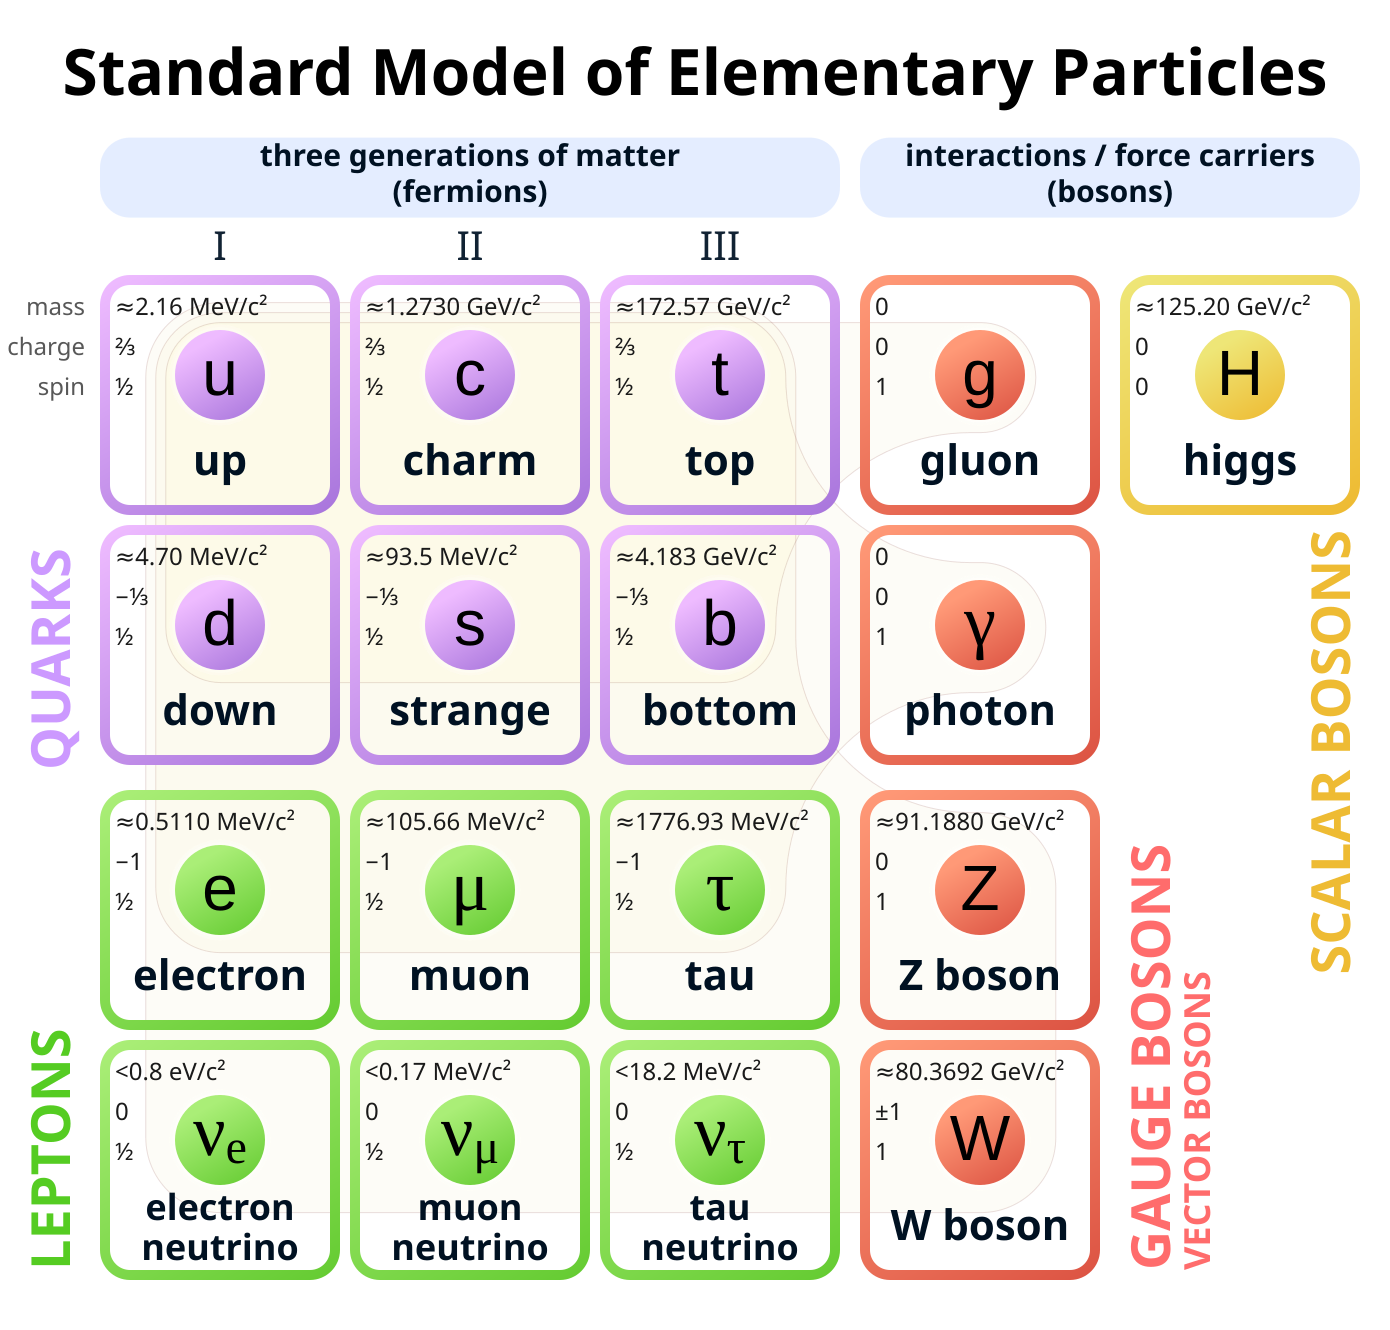
\includegraphics[width=0.8\textwidth]{figures/01-SM/sm_diagram.png}
	\caption{Particles and their classifications in the SM, reproduced from Ref.~\cite{enwiki:1238968997}.}
	\label{fig:01_sm}
\end{figure}

Each force is intimately tied to a symmetry in the SM, and particles are further distinguished by their behavior under these symmetries --- or, equivalently, how they are affected by this force.
Fermions are divided by those interacting (quarks) and not interacting (leptons) with the nuclear strong force, while each of their rows in Figure~\ref{fig:01_sm} further separates them by different ``charges'' under the weak force.
Additionally, each particle's mass and electric charge represent the strength of its interaction with the Higgs and electromagnetic fields, respectively.
Finally, we can see a mysterious \textit{almost}-symmetry: there are three copies, or ``flavors'' or ``generations'', of each fermion, which are entirely identical but for their masses (e.g. the electron, muon, and tau family of particles).
Such a structure may suggest the presence of new, yet-to-be-discovered forces tied to this symmetry.

The goal of Part~\ref{part:sm} is to make this picture more precise, and lay the theoretical foundation for the work discussed in this dissertation.
The mathematical frameworks needed to do so are called group theory and quantum field theory (QFT), and are the subjects of Chapters~\ref{sec:01_symmetries} and~\ref{sec:01_qft}, respectively.
Equipped with these tools, we then describe the SM in Chapter~\ref{sec:01_sm}, including the interactions discussed above and, of most relevance to the subject of this dissertation, the phenomenon of jets, the Higgs sector, and Higgs boson pair production within and beyond the SM.

These chapters build off of several great resources, including:
\begin{itemize}
	\item David Tong's extremely useful and insightful lecture notes on QFT~\cite{TongQFT}, gauge theories~\cite{TongGT}, and the standard model~\cite{TongSM};
	\item John McGreevy's great course on symmetry in physics~\cite{McGreevyGT} (which I had the pleasure of attending in the Fall of 2020);
	\item Frederic Schuller's precise lectures on the geometric anatomy of theoretical physics~\cite{SchullerGATP};
	\item Tony Zee's \textit{Group Theory in a Nutshell for Physicists}~\cite{Zee:2016fuk} and \textit{Quantum Field Theory in a Nutshell}~\cite{Zee:2003mt};
	\item Peskin and Schroeder's classic \textit{An Introduction to Quantum Field Theory}~\cite{Peskin:1995ev};
	\item Gavin Salam's lectures on \textit{Elements of QCD for hadron colliders}~\cite{Salam:2010zt};
	\item and Hong Liu~\cite{LiuRQFT} and Ricardo Matheus'~\cite{MatheusQFT} clear, recorded lectures on QFT.
\end{itemize}

\chapter{Symmetries in physics}
\label{sec:01_symmetries}

\begin{center}
	\centering
	\noindent
	\textit{Perfectly balanced, as all things should be.} --- Thanos
\end{center}

Symmetry is a powerful and beautiful way to understand nature. 
Intuitively, a symmetry is a transformation that leaves an object unchanged.
For example, a plain square has a four-fold rotational symmetry: it looks identical rotated once, twice, thrice, or four times by $90^{\circ}$.

Similarly, in physics, a symmetry is a transformation that leaves the laws of physics unchanged.
Electromagnetism, for example, is invariant to translations in space or time: electric charges and currents should behave the same in San Diego 5 years ago as in Geneva today.
Understanding such symmetries, and accounting for them in our mathematical formulation, has been a guiding principle in the development of the SM over the 20th century, and is one in understanding it as well.

In recent years, symmetries have also guided the development of machine learning algorithms in becoming more powerful and efficient.
A particular focus is placed in this dissertation on such \textit{equivariant} algorithms, which respect the symmetries and 
\textit{inductive biases} of our high energy physics data.
This chapter lays the foundation for these ideas, which we discuss in more detail in Chapter~\ref{sec:03_ml} and contribute to in Chapter~\ref{sec:06_lgae}.

In this chapter, we first introduce the framework for describing symmetries, group theory, in Section~\ref{sec:01_symmetries_gt}.
We then describe Lie algebras for continuous symmetries, and derive representations for the algebra corresponding to 3D rotations, in Section~\ref{sec:01_symmetries_so3}.
% in Sections~\ref{sec:01_symmetries_continuous} and~\ref{sec:01_symmetries_lie}, respectively.
% We then derive representations of the Lie algebra corresponding to 3D rotations in Section~\ref{sec:01_symmetries_so3}.
We conclude in Section~\ref{sec:01_symmetries_poincare} with a discussion of the Lorentz and Poincaré groups, comprising the fundamental symmetries of spacetime, whose irreducible representations are what we call particles.
% This  lays the foundations for describing \textit{group-equivariant} machine learning algorithms, an exciting area of research in AI that will be a focus of Chapter~\ref{sec:06_ml4jets}.

\section{Group theory}
\label{sec:01_symmetries_gt}

The mathematical formalism for describing symmetries is called \textit{group theory}.

\begin{definition}
\label{def:01_group}
The fundamental object in group theory is a \textit{group}, defined as a pair $(G, \bullet)$, where $G$ is a set and $\bullet: G \times G \rightarrow G$ is the group operation, which together satisfies the following properties:
\begin{enumerate}[i)]
	\item Associativity: $\forall a, b, c \in G: (a \bullet b) \bullet c = a \bullet (b \bullet c)$.
	\item Identity element: $\exists e \in G: \forall a \in G: a \bullet e = e \bullet a = a$.
	\item Inverse element: $\forall a \in G: \exists a^{-1} \in G: a \bullet a^{-1} = a^{-1} \bullet a = e$.
\end{enumerate}
\end{definition}

\begin{definition}
\label{def:01_abelian}
Note from Definition~\ref{def:01_group} that the group operation is not necessarily commutative ($\forall a, b \in G: a \bullet b = b \bullet a$).
If this condition does hold, the group is called an \textit{abelian} group.
\end{definition}

\begin{example}
\label{example:01_square}
To formalize the four-fold rotation symmetry of a square discussed above, we can define the group $\mathbb Z_4$  as ($\{0, 1, 2, 3\}$, $+_4$), where $+_4$ is addition modulo 4, and the elements of the set can represent rotations by $0^{\circ}$, $90^{\circ}$, $180^{\circ}$, and $270^{\circ}$, respectively.
One can check that $\mathbb Z_4$ satisfies all the properties of an abelian group.
\end{example}

\subsubsection{Group representations}

To make the abstract mathematical structure of the group more concrete, we next consider \textit{representations} of groups.

\begin{definition}
\label{def:01_representation}
A group representation $R$, of dimension $d$, is a mapping of the group elements to $d\times d$ matrices $D(g)$ in some $d$-dimensional vector space $V$, such that the group operation is preserved: $D(g_1)D(g_2) = D(g_1 \bullet g_2)$.
Necessarily, this means that $D(e) = \identity$, the identity matrix of $V$.
Representations of a group are not unique, and arbitrarily many new represenations can be constructed simply by taking tensor sums and products, denoted by the $\oplus$ and $\otimes$ symbols respectively, of existing ones.
\end{definition}

\begin{definition}
\label{def:01_irreps}
An \textit{irreducible representation} (irrep) is one with no non-trivial invariant subspaces, i.e., it cannot be decomposed into the tensor sums of smaller-dimensional representations.\footnote{Technically, certain pathological reducible representations of non-compact groups also cannot be decomposed into irreps, so ``non-decomposability'' is a necessary but insufficient condition for irreps.}
\end{definition}

\begin{example}
\label{example:01_square_representation}
The group $\mathbb Z_4$ from Example~\ref{example:01_square} can be represented simply as scalar complex numbers ($V = \mathbb C$):
\begin{equation}
	\label{eq:01_z4_representation}
	\begin{array}{cccc}
	0 & 1 & 2 & 3 \\
	\downarrow & \downarrow & \downarrow & \downarrow \\
	1 & e^{i\frac{\pi}{2}} & e^{i\pi} & e^{i\frac{3\pi}{2}}
	\end{array}
\end{equation}
One can check this satisfies the conditions of Definition~\ref{def:01_representation}, and since it is 1-dimensional, it is also irreducible.
\end{example}

\begin{definition}
\label{def:01_symmetry_regular_representation}
Every group has a $|G|$-dimensional \textit{regular representation} $R^{\mathrm{reg}}$, where $|G|$ is the number elements of the group, called the \textit{order} of the group.
The vector space $V = \mathrm{span}\{\ket{g}|g\in G\}$, and the representation is defined such that
\begin{equation}
	\label{eq:01_regular_representation}
	D^{\mathrm{reg}}(g)\ket{h} = \ket{gh}.
\end{equation}
\end{definition}

\begin{example}
\label{example:01_z4_regular}
For our $\mathbb Z_4$ group, we can use the set of four basis vectors $\{\ket{0} = \mathbf{e}_0, \ket{1} = \mathbf{e}_1, \ket{2} = \mathbf{e}_2, \ket{3} = \mathbf{e}_3\}$ in $\mathbb R^4$, and derive the matrices $D^{\mathrm{reg}}(g)$ such that they transform $\ket{g}$ according to the respective group operations:
\setlength{\arraycolsep}{10pt}
\begin{equation} \begin{split}
	\label{eq:01_z4_regular}
	D^{\mathrm{reg}}(0) &= \begin{pmatrix}
		1 & 0 & 0 & 0 \\
		0 & 1 & 0 & 0 \\
		0 & 0 & 1 & 0 \\
		0 & 0 & 0 & 1
	\end{pmatrix}, \quad
	D^{\mathrm{reg}}(1) = \begin{pmatrix}
		0 & 1 & 0 & 0 \\
		0 & 0 & 1 & 0 \\
		0 & 0 & 0 & 1 \\
		1 & 0 & 0 & 0
	\end{pmatrix}, \quad \\[1em]
	D^{\mathrm{reg}}(2) &= \begin{pmatrix}
		0 & 0 & 1 & 0 \\
		0 & 0 & 0 & 1 \\
		1 & 0 & 0 & 0 \\
		0 & 1 & 0 & 0
	\end{pmatrix}, \quad
	D^{\mathrm{reg}}(3) = \begin{pmatrix}
		0 & 0 & 0 & 1 \\
		1 & 0 & 0 & 0 \\
		0 & 1 & 0 & 0 \\
		0 & 0 & 1 & 0
	\end{pmatrix}.
\end{split} \end{equation}
\end{example}

The regular representation has some fun properties, such as its reducibility into irreps with each irrep appearing as many times in the decomposition as its dimension.
For us, it will mostly serve as a useful way to think about the \textit{adjoint} representation we will encounter below.

\subsubsection{Continuous symmetries}
\label{sec:01_symmetries_continuous}

Symmetries can be \textit{discrete}, as above, as well as continuous.

\begin{example}
\label{example:01_circle}
A circle has a continuous 2D rotational symmetry; rotations by any angle $\theta$ leave it invariant.
This corresponds to the \textit{special orthogonal} group in 2-dimensions $\SO[2]$.
\end{example}

\begin{definition}
\label{def:01_son}
More generally, the orthogonal group in $n$ dimensions, $\OO[n]$, is defined as	the group of orthogonal, or ``distance-preserving'', $n \times n$ matrices $M$, s.t. $MM^T = \identity$. 
The \textit{special orthogonal} group $\SO[n]$ is the subgroup of $n \times n$ orthogonal matrices with determinant 1, essentially retaining only rotations while removing reflections.
\end{definition}

As their definition suggests, the \SO[n] group elements have a natural representation as the $n \times n$ rotation matrices.
For \SO[2], these are of the form:
\begin{equation}
	\label{eq:01_so2}
	M(\theta) = \begin{pmatrix}
		\cos \theta & -\sin \theta \\
		\sin \theta & \cos \theta
	\end{pmatrix},
\end{equation}
where $\theta \in [0, 2\pi)$ is the angle of rotation.
These $n \times n$ matrix representations are called the \textit{fundamental} or \textit{defining} representations of \SO[n].

\begin{definition}
\label{def:01_sun}
\SO[2] is \textit{isomorphic} --- meaning identical to in terms of its group-theoretic properties --- to the \textit{unitary} group \UU[1].
The \textit{unitary} group \UU[n] is the group of $n \times n$ unitary matrices, i.e., those satisfying $M^\dagger M = MM^\dagger = \identity$, where $M^\dagger$ is the conjugate transpose, or Hermitian conjugate (h.c.) of $M$.
The special unitary group \SU[n], again is the subgroup of $n \times n$ unitary matrices with determinant 1.
As we will soon see, these groups effectively define the structure of the SM.
\end{definition}

\UU[1] has the simple 1D fundamental representation:
\begin{equation}
	\label{eq:01_u1}
	M(\theta) = e^{i\theta},
\end{equation}
i.e., all complex numbers of unit magnitude.


\begin{definition}
\label{def:01_compact}
An infinite group is \textit{compact} if a group-invariant sum or integral over the group elements is finite.
\UU[1] is compact, as
\begin{equation}
	\label{eq:01_u1_integral}
	\int_0^{2\pi} d\theta = 2\pi
\end{equation}
is finite. 
Indeed, all \SO[n] and \SU[n] groups are compact.
\end{definition}

Examples of important non-compact groups include the group of translations in $n$ dimensions and the Lorentz group, which we will discuss in detail in Section~\ref{sec:01_symmetries_poincare}.

\section{Lie algebras}
\label{sec:01_symmetries_lie}

We next introduce the concepts of Lie groups and Lie algebras, which are highly useful in understanding the structure and representations of continuous groups.

\begin{definition}
\label{def:01_lie_group}
A \textit{Lie group} is a group that is also a differentiable manifold, or ``smooth''.
Virtually all continuous groups we consider in physics are Lie groups.
What this means is that we can think of the operation of any arbitrary group element as equivalent to $N$ successive infinitesimal operations of the form 
\begin{equation}
	\label{eq:01_lie_group_infinitesimal}
	g(\varepsilon_A) = \identity + i \varepsilon_A T_A,
\end{equation}
where $\varepsilon_A$ are infinitesimal and indexing the continuous group parameters, e.g. rotation angles for \SO[n], $T_A$ are called the \textit{generators} of the group,
% \footnote{They are named so because they \textit{generate} the transformations of the group; for example, we will see that the generators for rotations correspond to angular momentum, which is what is required for a body to rotate.} 
and we are using Einstein notation, implicitly summing over the index $A$.
Thus, for a general element $g(\theta_A)$, where $\theta_A = N \varepsilon_A$ as defined above, we have
\begin{equation}
	\label{eq:01_lie_group_finite}
	g(\theta_A) = \left(\identity + i \frac{\theta_A}{N} T_A\right)^N \xrightarrow{N \rightarrow \infty} e^{i\theta_A T_A}.
\end{equation}
This is somewhat analogous to Taylor expansion in calculus, except for Lie groups only the first order / derivative term is necessary to capture the group behavior.\footnote{This is because, based on the Campbell-Baker-Hausdorff~\cite{enwiki:1183926638} formula, higher order terms in the expansion of exponential form of $g$ in Eq.~\ref{eq:01_lie_group_finite} involve only commutators of the generators.}
% More importantly, the generators $T_A$ are highly useful in understanding the structure and representations of the Lie group.
\end{definition}

\begin{definition}
\label{def:01_lie_algebra}
The \textit{Lie algebra}, $\mathfrak{g}$, of a group is defined by the set of commutation relations between its generators:\footnote{An \textit{algebra} $(V, \bullet)$ is a vector space $V$ with a bilinear operation $\bullet: V \times V \rightarrow V$.
Examples include the cross product of vectors and matrix multiplication of square matrices.
The Lie algebra is the special case where $\bullet$ is the commutator.}
\begin{equation}
	\label{eq:01_lie_algebra}
	[T_A, T_B] = i f_{ABC} T_C,
\end{equation}
where $[T_A, T_B] = T_A T_B - T_B T_A$ is the commutator of $T_A$ and $T_B$, and $f_{ABC}$ are called the \textit{structure constants} of $\mathfrak{g}$.
As $[T_A, T_B] = -[T_B, T_A]$, the structure constants must be totally antisymmetric in the swapping of their indices.
% Commutators also carry the following useful property, known as the Jacobi identity:
% \begin{equation}
% 	\label{eq:01_jacobi}
% 	[T_A, [T_B, T_C]] + [T_B, [T_C, T_A]] + [T_C, [T_A, T_B]] = 0.
% \end{equation}
\end{definition}

\begin{example}
\label{example:01_u1_lie}
For the \UU[1] group,  we can see directly from Eq.~\ref{eq:01_u1} that the sole generator of the group is $T = 1$.
This has the rather uninteresting Lie algebra $\mathfrak{u}(1)$ of $[1, 1] = 0$, stemming from the fact that the group is abelian.
Next, we look at the more interesting \SO[3] and \SU[2] groups, where the power of Lie algebras shines.
\end{example}


% \subsection{Representations of the \texorpdfstring{\so[3] and \su[2]}{so(3) and su(2)} algebras}
\label{sec:01_symmetries_so3}

\subsubsection{Fundamental and adjoint representations of the \so[3] and \su[2] algebras}

We now turn to the derivation of the Lie algebras and representations of the \SO[3] and \SU[2] groups, both because of their importance in physics, and because the derivation introduces a number of useful concepts and definitions for the following sections.
\SO[3] and \SU[2] are very closely related: \SU[2] is a \textit{double cover} of \SO[3], which means that every rotation in \SO[3] can be mapped to two elements of \SU[2].
Importantly, however, they are locally isomorphic near the identity, meaning they have the same Lie algebra.

We can derive the generators of \SO[3] by using the properties of the special orthogonal group ($R^TR=\identity$).
From Eq.~\ref{eq:01_lie_group_infinitesimal}, we have
\begin{equation} 
	\begin{split}
	\label{eq:01_so3_generators_derivation}
	R(\varepsilon) &\approxeq \identity + i \varepsilon T \\
	R^TR &= \identity + i \varepsilon (T^T + T) + \mathcal O(\varepsilon^2) \mustequal \identity \\
	\Rightarrow T^T &= -T.
\end{split} 
\end{equation}
Thus $T$ are antisymmetric matrices, of which for $N = 3$ dimensions there are three linearly independent ones:
\begin{equation}
	\label{eq:01_so3_generators}
	J_x = i\begin{pmatrix}
		0 & 0 & 0 \\
		0 & 0 & -1 \\
		0 & 1 & 0
	\end{pmatrix}, \quad
	J_y = i\begin{pmatrix}
		0 & 0 & 1 \\
		0 & 0 & 0 \\
		-1 & 0 & 0
	\end{pmatrix}, \quad
	J_z = i\begin{pmatrix}
		0 & -1 & 0 \\
		1 & 0 & 0 \\
		0 & 0 & 0
	\end{pmatrix},
\end{equation}
labeled as $x$, $y$, $z$ as they represent rotations around the respective axes.
The factor of $i$ ensures the reality of the infinitesimal rotations in Eq.~\ref{eq:01_so3_generators_derivation} and also that the generators are Hermitian.\footnote{Note that the conventions around this factor are inconsistent in the literature and likely, despite our best efforts, will be inconsistent in this chapter as well.}
These provide us with the fundamental representation of \so[3], and should be familiar as the angular momentum operators in quantum mechanics (QM).
By exponentiating these, as in Eq.~\ref{eq:01_lie_group_finite}, we obtain the fundamental representation of the \SO[3] group: $R(\vec{\theta}) = e^{i\theta_i J_i}$.
% Note that conventions around the factor of $i$ in the representations and commutation relations are annoyingly inconsistent in the literature and likely, despite our best efforts, in this chapter as well.

To find the fundamental representation of \su[2], we can follow the same procedure as above, using the unitarity constraint $R^\dagger R = \identity$ for $N = 2$ dimensional complex matrices, which yields:
\begin{equation} 
	\label{eq:01_su2_generators}
	\begin{split}
	\setlength{\arraycolsep}{8pt}
	T_1 = \frac{1}{2}\sigma_x = \frac{1}{2}\begin{pmatrix}
		0 & 1 \\
		1 & 0
	\end{pmatrix}, \quad
	&T_2 = \frac{1}{2}\sigma_y = \frac{1}{2}\begin{pmatrix}
		0 & -i \\
		i & 0
	\end{pmatrix}, \\[1em]
	T_3 = \frac{1}{2}\sigma_z = &\frac{1}{2}\begin{pmatrix}
		1 & 0 \\
		0 & -1
	\end{pmatrix},
\end{split} 
\end{equation}
where $\sigma_i$ are the Pauli matrices --- the angular momentum operators for the spin of spin-$1/2$ particles in QM.
Either set of generators yield the following Lie algebra of both groups:
\begin{equation}
	\label{eq:01_so3_su2_lie_algebra}
	[T_A, T_B] = i \epsilon_{ABC} T_C,
\end{equation}
where the structure constants $f_{ABC}$ of the algebra are simply $\epsilon_{ABC}$, the totally antisymmetric Levi-Civita tensor.

Structure constants themselves furnish the following representation of the corresponding Lie algebra:
\begin{equation}
	\label{eq:01_adjoint}
	[T_A]_{BC} = -i f_{ABC}.
\end{equation}
This can be confirmed by plugging this representation into the commutator in Eq.~\ref{eq:01_lie_algebra} and using the Jacobi identity~\cite{Jacobi1862}.
As $B, C$ index the number of generators, we see that this representation has a dimension equal to the number of generators of the Lie algebra, and it is called its \textit{adjoint} representation.
It is analogous to the regular representation (Definition~\ref{def:01_symmetry_regular_representation}) for a Lie algebra, with the underlying vector space spanned by the generators $V = \mathrm{span}\{\ket{T_A}\}$ and the requirement that $D(T_A)\ket{T_B} = i f_{ABC} \ket{T_C}$.

\begin{definition}
\label{def:01_lie_group_dim}
The dimension of a Lie group is defined as the number of generators of the group.
Thus, it is the same as the dimension of the adjoint representation.
\end{definition}

As it turns out, for \so[3] and \su[2], the adjoint representation $[T_A]_{BC} = -i \varepsilon_{ABC}$ is simply the fundamental representation of \so[3].
More generally, the dimensions of the fundamental and adjoint representations of \SO[n] and \SU[n] are given in Tab.~\ref{tab:01_so_su_dimensions}.	
The significance of these representations, as we will see, is that the force carriers (i.e., gauge bosons) of the SM live in the adjoint representation of their associated gauge group, while the matter particles live in either their fundamental or trivial representations.

\begin{table}[ht!]
	\centering
	\renewcommand{\arraystretch}{1.5}
	\setlength{\tabcolsep}{10pt}
	\begin{tabular}{c|c|c}
		\textbf{Group} & \textbf{dim(Fundamental)} & \textbf{dim(Adjoint)} \\
		\hline
		% \SO[2] & 1 & 1 \\
		% \SO[3] & 3 & 3 \\
		\SO[n] & $n$ & $n(n-1)/2$ \\
		% \SU[2] & 2 & 3 \\
		% \SU[3] & 3 & 8 \\
		\SU[n] & $n$ & $n^2 - 1$ \\
	\end{tabular}
	\vspace{1em}
	\caption{Dimensions of the fundamental and adjoint representations of the \SO[n] and \SU[n] groups.}
	\label{tab:01_so_su_dimensions}
\end{table}

\subsubsection{General representations}

So far we have discussed two representations of the \so[3] and \su[2] algebras.
The general representations can be derived in much the same way as finding the eigenstates of the angular momentum operator in QM.
We first choose a basis in which one of the generators, conventionally $J_z$, is diagonal, and label eigenvectors of $J_z$ as $\ket{m}$ with eigenvalue $m$:
\begin{equation}
	\label{eq:01_so3_su2_eigenstates}
	J_z\ket{m} = m\ket{m}.
\end{equation}
These eigenvectors, by definition, form a basis for the representations of the generators, so counting them tells us the dimensions of allowed representation.
To do so, we define the ``raising'' and ``lowering'' operators $J_{\pm} = J_x \pm i J_y$, with commutation relations
\begin{equation}
	\label{eq:01_so3_su2_raise_lower}
	[J_z, J_{\pm}] = \pm J_{\pm}, \quad [J_+, J_-] = 2J_z.
\end{equation}
These are named so because
\begin{equation}
	\label{eq:01_so3_su2_raise_lower_eigenstates}
	J_zJ_\pm\ket{m} = [J_\pm Jz \pm J_\pm]\ket{m} = (m \pm 1)J_\pm\ket{m},
\end{equation}										
i.e., $J_\pm\ket{m}$ are eigenvectors of $J_z$ with eigenvalues $m \pm 1$, implying
\begin{equation}
	\label{eq:01_so3_su2_raise_lower_operation}
	J_\pm\ket{m} = c^\pm_{m\pm1}\ket{m \pm 1},
\end{equation}
where $c_{m\pm1}$ are normalization constants.
Now if we assume that the representation is finite-dimensional and label the highest-weight state $\ket{j}$ --- such that $J_+\ket{j} = 0 \Leftrightarrow c^+_{j+1} = 0$ --- we can iteratively lower the state and solve for the normalization constants until we reach the lowest-weight state.
By doing so we find that $c^-_{-j-1} = 0 \Rightarrow$ the lowest weight state is in fact $\ket{-j}$.\footnote{See, for example, Chapter IV.2 in Zee~\cite{Zee:2016fuk} for a more detailed derivation.}

Thus, we conclude the algebra allows $2j+1$-dimensional representations spanned by $\{\ket{-j}, \ket{-j+1}, \ldots, \ket{j-1}, \ket{j}\}$, with $j \in \mathbb Z^{\geq0}/2$ (non-negative integers and half-integers only).
Each possible $j$ indexes a different representation of the group, and any eigenstate can thus be labeled by $\ket{j, m}$.
We have already seen the $j = 1/2$ and $j = 1$ representations explicitly in Eqs.~\ref{eq:01_su2_generators} and \ref{eq:01_so3_generators}, respectively, while the $j = 0$ is simply the trivial representation of the group ($D(g) = 1 \,\ \forall g \in G$).

\begin{definition}
\label{def:01_casimir}
More generally, irreducible representations of a group are labeled by eigenvalues of the \textit{Casimir invariants}, or Casimirs, of the group.
Casimirs are operators that commute with all generators of the group.
For \so[3] and \su[2], there is only one Casimir,
\begin{equation}
\label{eq:01_so3_su2_casimir}
J^2 = J_x^2 + J_y^2 + J_z^2.
\end{equation}
This is the total angular momentum operator, which we know from QM commutes with all the $J_i$s and for any eigenstate $\ket{j, m}$ has eigenvalue $j(j+1)$:
\begin{equation}
\label{eq:01_so3_su2_casimir_eigenvalue}
J^2\ket{j, m} = j(j+1)\ket{j, m}.
\end{equation}
As expected, since the Casimir commutes with all the generators, its eigenvalues depend only on the irrep $j$.
We have also seen that individual states can be further labeled using the eigenvalues of a set of maximally commuting operators, in this case $\{J^2, J_z\}$.
\end{definition}

These representations can directly be used to derive those corresponding to the \SU[2] and \SO[3] group except that, surprisingly, the latter does not admit the half-integer irreps; essentially, \SU[2] has double the irreps because it is the double cover of \SO[3].
Overall, the irreps of \su[2] and \su[3] are quite significant in physics, with direct applications to classical and quantum mechanics, and, moreover, they will also serve as the building blocks for the representations of the Lorentz and Poincaré groups in the next section.

\section{Particles are irreps of the Poincaré group}
\label{sec:01_symmetries_poincare}

The Poincaré group comprises all the physical symmetries of ``flat'' spacetime (i.e, without gravity), i.e. all the transformations which leave the laws of physics invariant.
These include Lorentz transformations (boosts and rotations) and spacetime translations.

Particles can be defined as a ``set of states which mix only among themselves under Poincaré transformations'' (Schwartz~\cite{Schwartz:2014sze} Ch. 8.1), leaving attributes like their mass and spin invariant.
Elementary particles are those for which there is no smaller subset of states that also have this property.
Thus, they correspond exactly to irreducible representations of the Poincaré group!
That the physical and seemingly nebulous concept of a particle can be so precisely defined and characterized by a mathematical analysis of the symmetries of spacetime is one of the most beautiful results of fundamental physics.

In this section, we describe the irreps of the Poincaré group, starting first with the Lorentz group alone.

% \subsection{Representations of the Lorentz group}

\subsubsection{The (proper, orthochronous) Lorentz group}

We know from special relativity that ``flat'' spacetime (i.e., without gravity) is described by 4D Minkowski space $\mathbb R^{1, 3}$.
This is a real vector space equipped with the metric $\eta_{\mu\nu} = \mathrm{diag}(1, -1, -1, -1)$, which defines distances, or inner products $\langle \cdot, \cdot \rangle$, between 4-vectors $x_\mu = (x_0, x_1, x_2, x_3)$ as:
\begin{equation}
	\label{eq:01_minkowski_metric}
	\langle x, y \rangle \equiv x_\mu y^\mu \equiv \eta_{\mu\nu}x^\mu y^\nu = x_0 y_0 - x_1 y_1 - x_2 y_2 - x_3 y_3.
\end{equation}

\begin{definition}
\label{def:01_lorentz_group}
% Lorentz transformations are those which preserve the magnitude of 4-vectors in Minkowski space $\mathbb R^{1, 3}$.
The \textit{Lorentz group} is the group of all matrices $M$ orthogonal under the Minkowski metric $M^T\eta M = \eta$, and is called \OO[1, 3].
This is the analog in flat spacetime to distance-preserving transformations in Euclidean space (e.g., \OO[3]).
\end{definition}

\begin{definition}
\label{def:01_proper_orthochronous}
The \textit{proper, orthochronous} Lorentz group $\mathrm{SO}^+(1, 3)$ is the subgroup of \OO[1, 3] matrices continuously connected to the identity.
Physically, these are the transformations that preserve the orientation of space and direction of time, and are typically what we refer to as \textit{Lorentz transformations}.
The two transformations of \OO[1, 3] not included in $\mathrm{SO}^+(1, 3)$ are parity $P = \diag(1, -1, -1, -1)$ and time reversal $T = \diag(-1, 1, 1, 1)$ (shown in the 4-vector representation), which flip the sign of spatial and temporal components of 4-vectors, respectively.
Surprisingly, these are not symmetries of nature ---
they are violated by the weak interaction!
% \TODO{We discuss this more in ...}
Generally, in this chapter, when we talk about the Lorentz group or Lorentz invariance, we are referring only to the proper, orthochronous Lorentz group.
\end{definition}

\subsubsection{Generators of the Lorentz group}

Lorentz transformations $\Lambda$ are generated by six antisymmetric matrices, three for boosts ($K_i$) and three for rotations ($J_i$).
In the $4$-vector representation, these are:
\begin{equation} 
	\begin{split}
	\label{eq:01_lorentz_generators}
	K_x &= -i\begin{pmatrix}
		\setlength{\arraycolsep}{10pt}
		0 & 1 & 0 & 0 \\
		1 & 0 & 0 & 0 \\
		0 & 0 & 0 & 0 \\
		0 & 0 & 0 & 0
	\end{pmatrix}, \ 
	K_y = -i\begin{pmatrix}
		0 & 0 & 1 & 0 \\
		0 & 0 & 0 & 0 \\
		1 & 0 & 0 & 0 \\
		0 & 0 & 0 & 0
	\end{pmatrix}, \ 
	K_z = -i\begin{pmatrix}
		0 & 0 & 0 & 1 \\
		0 & 0 & 0 & 0 \\
		0 & 0 & 0 & 0 \\
		1 & 0 & 0 & 0
	\end{pmatrix}, \\[1em]
	\setlength{\arraycolsep}{5pt}
	J_x &= i\begin{pmatrix}
		0 & 0 & 0 & 0 \\
		0 & 0 & 0 & 0 \\
		0 & 0 & 0 & -1 \\
		0 & 0 & 1 & 0
	\end{pmatrix}, \ 
	J_y = i\begin{pmatrix}
		0 & 0 & 0 & 0 \\
		0 & 0 & 0 & 1 \\
		0 & 0 & 0 & 0 \\
		0 & -1 & 0 & 0
	\end{pmatrix}, \ 
	J_z = i\begin{pmatrix}
		0 & 0 & 0 & 0 \\
		0 & 0 & -1 & 0 \\
		0 & 1 & 0 & 0 \\
		0 & 0 & 0 & 0
	\end{pmatrix}.
\end{split} 
\end{equation}
Lorentz transformations can thus be represented as
\begin{equation}
	\label{eq:01_lorentz_generators_exponential}
\Lambda(\vec{\theta}, \vec{\beta}) = e^{i(\theta_i J_i + \beta_i K_i)},
\end{equation}
where $\vec{\theta}$ and $\vec{\beta}$ are the rotation and boost parameters, respectively,
% Note that these only represent the transformations of the Lorentz group continuously connected to the identity (by definition of the Lie algebra, Definition~\ref{def:01_lie_algebra}).

An important property of the Lorentz group is that it is not compact.
This is related to the fact that the generators for boosts $K_i$ in the representation above are not Hermitian, which means the corresponding group elements $e^{i\beta_i K_i}$ are not unitary.
In fact, there are no finite-dimensional unitary representations of the Lorentz group~\cite{Wigner:1939cj}.
Unitarity of operators is an important condition for the invariance of physical properties under transformations in QM, and the consequences of this for the SM will be discussed in Chapter~\ref{sec:01_qft_spinors}.

\subsubsection{Lie algebra of the Lorentz group}

From Eq.~\ref{eq:01_lorentz_generators}, we can derive the commutation relations of the generators and, hence, the Lie algebra:
\begin{equation}
	\begin{split}
		\label{eq:01_lorentz_algebra}
		[K_i, K_j] &= -i \epsilon_{ijk} J_k, \\
		 [J_i, J_j] &= i \epsilon_{ijk} J_k, \\
		[J_i, K_j] &= i \epsilon_{ijk} K_k.
	\end{split}
\end{equation}
Moreover, if we define the operators
\begin{equation}
	\label{eq:01_lorentz_su2_operators}
	J^+_i = \frac{1}{2}(J_i + iK_i), \quad J^-_i = \frac{1}{2}(J_i - iK_i),
\end{equation}
we find that \so[1, 3] contains two mutually commuting \su[2] subalgebras:
\begin{equation}
	\begin{split}
		\label{eq:01_lorentz_su2_subalgebras}
		[J^+_i, J^+_j] &= i \epsilon_{ijk} J^+_k, \\
		[J^-_i, J^-_j] &= i \epsilon_{ijk} J^-_k, \\
		[J^+_i, J^-_j] &= 0.
	\end{split}
\end{equation}
This implies the irreps of \so[1, 3] are simply two copies of the irreps of \su[2] from Section~\ref{sec:01_symmetries_so3}, indexed as $(j_1, j_2)$ with $j_1, j_2 \in \mathbb Z^{\geq0}/2$ and dimension $(2j_1 + 1)(2j_2 + 1)$.

With this, we can easily obtain the generators $J_i$, $K_i$ for the smallest few irreps:
% \begin{itemize}
% 	\item $(0, 0)$: \quad $J^+_i = J^-_i = 0 \Rightarrow J_i = K_i = 0$.
% 	\item $(1/2, 0)$: \quad $J^+_i = \frac{1}{2} \sigma_i$, $J^-_i = 0 \Rightarrow J_i = \frac{1}{2} \sigma_i$, $K_i = -\frac{i}{2} \sigma_i$.
% \end{itemize}
\begin{align}
	\label{eq:01_lorentz_irreps_00}
	(0, 0)\text{:}& \qquad J^+_i = J^-_i = 0 \! &\Rightarrow& \qquad J_i = K_i = 0. \\
	\label{eq:01_lorentz_irreps_weyl_left}
	(\nicefrac{1}{2}, 0)\text{:}& \qquad J^+_i = \frac{1}{2} \sigma_i,\, J^-_i = 0 \! &\Rightarrow& \qquad J_i = \frac{1}{2} \sigma_i, K_i = -\frac{i}{2} \sigma_i. \\
	\label{eq:01_lorentz_irreps_weyl_right}
	(0, \nicefrac{1}{2})\text{:}& \qquad J^+_i = 0,\, J^-_i = \frac{1}{2} \sigma_i \! &\Rightarrow& \qquad J_i = \frac{1}{2} \sigma_i, K_i = \frac{i}{2} \sigma_i. \\[2mm]
	% (\nicefrac{1}{2}, \nicefrac{1}{2})\text{:}& 
	& \qquad\qquad\qquad\qquad\qquad \vdots \notag
	\vspace{-10mm}
\end{align}
% \vspace{-2mm}
% As you can see, the $(\nicefrac{1}{2}, 0)$ and $(0, \nicefrac{1}{2})$ irreps are quite similar, and are called the \textit{left-} and \textit{right-handed Weyl spinor} representations, where the handedness refers to the direction of a particle's spin angular momentum relative to its momentum.
% are the left- and right-handed Weyl spinors, respectively, of the Lorentz group.
The $(\nicefrac{1}{2}, \nicefrac{1}{2})$ irrep is actually our familiar $4$-vector representation, but it is more involved to recover the generators in the same form as Eq.~\ref{eq:01_lorentz_generators}.\footnote{See e.g. Ref.~\cite{439080}.}

% For example, $(0, 0)$ is the trivial representation, with $J^+_i = J^-_i = 0 \Rightarrow J_i = K_i = 0$.
% The $(1/2, 0)$ representation means $J^+_i = \frac{1}{2} \sigma_i$, $J^-_i = 0 \Rightarrow J_i = \frac{1}{2} \sigma_i$, $K_i = -\frac{i}{2} \sigma_i$, while in $(0, 1/2)$, $J^+_i = 0$, $J^-_i = \frac{1}{2} \sigma_i \Rightarrow J_i = \frac{1}{2} \sigma_i$, $K_i = \frac{1}{2} \sigma_i$.

\subsubsection{Representations of the Lorentz group}

It turns out the above four irreps of the Lorentz group are all we need for the SM.
Their nomenclature and corresponding elementary particle fields are listed in Table~\ref{tab:01_lorentz_representations}.
Notably, fermions are classified as those with half-integer total spin $j = j_1 + j_2$, and bosons with integer $j$.
Their radically different behavior is a consequence of the Spin-Statistics theorem~\cite{PhysRev.110.1450} (a notoriously difficult theorem to prove~\cite{FeynmanVol3}), which states that half-integer spin particles obey Fermi-Dirac statistics and integer spin particles Bose-Einstein statistics.

All known fermionic particle fields live in the $(\nicefrac{1}{2}, 0) \oplus (0, \nicefrac{1}{2})$, or \textit{Dirac spinor}, representation.
The $(\nicefrac{1}{2}, 0)$ and $(0, \nicefrac{1}{2})$ representations are called the \textit{left-} and \textit{right-handed Weyl spinors} respectively, where the handedness refers to the direction of their spin angular momentum relative to their momentum.
Physically, this means there is a left-handed and right-handed copy of each fermion, and they have to be packaged together in a Dirac spinor to have masses without violating parity, as we discuss in Chapter~\ref{sec:01_qft_spinors}.
% \footnote{More fundamentally, this is necessary to resolve gauge anomalies that arise from the quantization of QED and QCD (see Tong SM~\cite{TongSM} Chapter 4.1).}
% The Dirac spinor thus comprises both a left-handed and right-handed component, which is necessary for QED- and QCD-\textit{gauge-invariant} fermion masses.\footnote{More fundamentally, this is necessary to resolve gauge anomalies that arise from the quantization of QED and QCD (see Tong SM~\cite{TongSM} Chapter 4.1).}
We will also see that left- and right-handed representations can be equivalently thought of as particles and antiparticles.

The $(\nicefrac{1}{2}, 0) \oplus (0, \nicefrac{1}{2})$ representation technically also includes real \textit{Majorana spinors} as a subspace, which can represent neutral fermions.
The only candidate for these in the SM are right-handed neutrinos and, in fact, the existence of such Majorana neutrinos could potentially explain the curiously small \textit{left-handed} neutrino masses through a process called the \textit{seesaw mechanism}~\cite{Foot:1988aq, Schechter:1980gr}.
To date, however, no experimental evidence for these, such as neutrinoless double beta decay~\cite{Rodejohann:2011mu} or same-sign charged dilepton decays~\cite{CMS:2018jxx}, has been observed.

On another technical note, the Lorentz group, similar to \SO[3], does not itself admit half-integer, fermionic representations.
Thus, the true spacetime symmetry group is actually the double cover of \SO[1, 3], $\mathrm{Spin}(1,3)$!
Indeed, there are many subtleties to the Lorentz group, some of which will be revisited in the context of Lorentz-group equivariant neural networks in Chapter~\ref{sec:06_lgae}.
To conclude, however, it is worth emphasizing again the remarkable physical insight these seemingly abstract group-theoretic concepts deliver.
We are able to classify a fundamental dichotomy of particle physics --- bosons versus fermions, and their completely different behavior --- simply by their representation under the Lorentz (or, rather, the $\mathrm{Spin}(1,3)$) group!

\begin{table}[ht!]
	\centering
	\renewcommand{\arraystretch}{1.5}
	% \setlength{\tabcolsep}{8pt}
	% wrap table to textwidth
	% \begin{wraptable}{r}{0.5\textwidth}
	\resizebox{\textwidth}{!}{
	\begin{tabular}{c|c|c}
		% \toprule
		\textbf{Representation $(j_1, j_2)$} & \textbf{Name} & \textbf{Elementary Fields} \\
		\hline
		$(0, 0)$ & Scalar & Higgs boson \\
		$(\nicefrac{1}{2}, 0)$ & Left-handed Weyl spinor & --- \\
		$(0, \nicefrac{1}{2})$ & Right-handed Weyl spinor & --- \\
		$(\nicefrac{1}{2}, 0) \oplus (0, \nicefrac{1}{2})$ & Dirac spinor & All fermions \\
		$(\nicefrac{1}{2}, \nicefrac{1}{2})$ & Vector & $g, \gamma, W^\pm,$ and $Z$ gauge bosons \\
		% \bottomrule
	\end{tabular}
	}
	\vspace{1em}
	\caption{Representations of the Lorentz group and their associated particle fields in the SM.}
	\label{tab:01_lorentz_representations}
\end{table}

% \subsection{Representations of the Poincaré group}

\subsubsection{Lie algebra of the Poincaré group}

The Poincaré group is Lorentz transformations plus spacetime translations.
Just as angular momentum generates rotations, translations are generated by the momentum operator $P_\mu$.
$P_\mu$ and the Lorentz generators $J_i$ and $K_i$ together comprise the generators of the Poincaré group, and its algebra is thus the Lorentz algebra (Eq.~\ref{eq:01_lorentz_algebra}) plus the commutation relations with the $P_\mu$s:\footnote{See Appendix~\ref{app:01_poincare_algebra} for a derivation.}
\begin{equation}
	\label{eq:01_poincare_algebra}
	\begin{split}
		[P_\mu, P_\nu] &= 0, \\
		[J_i, P_0] &= 0, \\
		[J_i, P_j] &= i \epsilon_{ijk}P_k, \\
		[K_i, P_0] &= -i P_i, \\
		[K_i, P_j] &= i \eta_{ij}P_0.
	\end{split}
\end{equation}
As is conventional, the Greek indices run over all four spacetime dimensions, while the Latin indices only the three spatial.

The Poincaré algebra can be expressed more compactly by first combining the Lorentz generators into the antisymmetric tensor $M_{\mu\nu}$:
\begin{equation}
\label{eq:01_lorentz_generators_mmunu}
M_{\mu\nu} = \begin{pmatrix}
	0 & K_x & K_y & K_z \\
	-K_x & 0 & J_z & -J_y \\
	-K_y & -J_z & 0 & J_x \\
	-K_z & J_y & -J_x & 0
\end{pmatrix}
\quad\Rightarrow \Lambda(\omega) = e^{\frac{i}{2}\omega^{\mu\nu} M_{\mu\nu}},
\end{equation}
% M_{0i} = -M_{i0} = K_i, \quad M_{ij} = \epsilon_{ijk} J_k \quad\Rightarrow \Lambda(\omega) = e^{\frac{i}{2}\omega^{\mu\nu} M_{\mu\nu}},
with $\omega_{\mu\nu}$ another antisymmetric tensor containing the six rotation and boost parameters.
The algebra can be then written as:
\begin{equation}
	\begin{split}
		\label{eq:01_poincare_algebra_mmunu}
		[M_{\mu\nu}, M_{\rho\sigma}] &= i(\eta_{\nu\rho}M_{\mu\sigma} - \eta_{\mu\rho}M_{\nu\sigma} - \eta_{\nu\sigma}M_{\mu\rho} + \eta_{\mu\sigma}M_{\nu\rho}), \\
		[M_{\mu\nu}, P_\rho] &= i(\eta_{\nu\rho}P_\mu - \eta_{\mu\rho}P_\nu), \\
		[P_\mu, P_\nu] &= 0.
	\end{split}
\end{equation}

\subsubsection{Irreps of the Poincaré group}

As we saw from Section~\ref{sec:01_symmetries_so3}, we can derive the irreps of an algebra using its Casimir invariants (Definition~\ref{def:01_casimir}).
Each set of their eigenvalues uniquely labels an irrep, while each basis state within the irreps is indexed by eigenvalues of a maximal set of commuting operators (e.g., $\{J^2, J_z\} \rightarrow \ket{j, m}$ for \so[3]).
Note that in the following, we simply provide a sketch of the derivations and point to, for example, Zee GT~\cite{Zee:2016fuk} Chapter VII.2 and Tong SM~\cite{TongSM} Chapter 1.1.2 for more detailed proofs and discussion.

The Casimirs of the Poincaré algebra are the operators
\begin{equation}
	\label{eq:01_poincare_casimirs}
	P^2 = P_\mu P^\mu\ \mathrm{ and }\ W^2 = W_\mu W^\mu,
\end{equation}
where 
\begin{equation}
	\label{eq:01_poincare_wmu}
	W_\mu = \frac{1}{2}\epsilon_{\mu\nu\rho\sigma}M^{\nu\rho}P^\sigma
\end{equation}
is the \textit{Pauli-Lubanski vector}, the relativistic analog of the angular momentum operator $J_i$.
Furthermore, $P_\mu$ commutes with both, and we can label its eigenstates as $\ket{p}$,
\begin{equation}
	\label{eq:01_poincare_pmu_eigenstates}
	P_\mu\ket{p} = p_\mu\ket{p}, 
\end{equation}
which represent single-particle states with 4-momentum $p_\mu$.
% Note that we have an infinite number of states and, therefore, necessarily infinite-dimensional representations of the Poincaré group because it is not compact.
These are therefore eigenstates of $P^2$ as well, with eigenvalues $m^2$, the squared mass of the particle:
\begin{equation}
	\label{eq:01_poincare_p2}
	P^2\ket{p} = p_\mu p^\mu\ket{p} = m^2 \ket{p}.
\end{equation}
Thus, we see that the mass of a particle, $m$, is one label of the irreps, with states therein indexed by $p_\mu$.
The other label, the particle spin $j$, is based on the eigenvalue of $W^2$:
\begin{equation}
	\label{eq:01_poincare_w2}
	W^2\ket{p, j} \propto j(j+1)\ket{p, j}.
\end{equation}
The easiest way to see this is to, for a given $m > 0$, pick a single eigenstate $\ket{p^*}$.
The simplest is the rest frame $p^*_\mu = (m, 0, 0, 0)$.
The subgroup of Poincaré transformations which leave $\ket{p^*}$ invariant is called its \textit{little group}.
In this case, it comprises all 3D rotations --- i.e., \SO[3].
Indeed, if we look at the Pauli-Lubanski vector acting on $\ket{p^*}$,
\begin{equation}
	\label{eq:01_poincare_w2_eigenstates}
	W_\mu\ket{p^*} = \frac{1}{2}\epsilon_{\mu\nu\rho\sigma}M^{\nu\rho}p^{*\sigma}\ket{p^*} \quad\Rightarrow W_0 = 0, W_i = -m J_i,
\end{equation}
we simply recover the generators $J_i$ of \so[3].\footnote{This also motivates why $W_\mu$ can be thought of as relativistic angular momentum.}
Therefore,
\begin{equation}
	\label{eq:01_poincare_w2_eigenvalues}
	W^2\ket{p^*, j} = m^2 J^2 \ket{p^*, j} = m^2j(j+1)\ket{p^*, j},
\end{equation}
using the eigenvalues of $J^2$ from Eq.~\ref{eq:01_so3_su2_casimir_eigenvalue}.
Although we chose here to look at a specific state $\ket{p^*}$, this can be shown to hold for all states $\ket{p}$ in the irrep.\footnote{By choosing an eigenstate $\ket{p^*, j}$ of $P^2$ and looking for transformations which leave it invariant, we ``induced'' a subgroup, \SO[3], and used its representation theory to derive the irreps of the Poincaré group. Such a representation is hence called an \textit{induced representation}.}
Thus, we see that irreps of the Poincaré group, and, hence, particles, are characterized by their mass $m$ and spin $j$.

\subsubsection{Massive versus massless particles}

Continuing with the massive, $m > 0$, particle case, we know as well from Section~\ref{sec:01_symmetries_so3} that the eigenstates within the $\ket{p, j}$ irreps are further labeled by their spin along a particular axis: $J_z\ket{p, j, m_j} = m_j\ket{p, j, m_j}$, with $m_j \in \{-j, -j+1, \ldots, j-1, j\}$.
Thus, massive particles $\ket{m, j}$ exist in $2j+1$ spin states $\otimes$ an infinite number of momentum states $\ket{p},\ p_\mu p^\mu = m^2$.

However, this is not the case for \textit{massless} particles, which have a different little group.
Recall that we can never boost into the rest frame of a massless particle to define the simple $\ket{p^*}$ we did above.
Instead, let us consider the next-best state $\ket{p'}$, $p'_\mu = (E, 0, 0, E)$.
% It is clearly left invariant by rotations in the $x-y$ plane, but also by two translations generated by:
% \begin{equation}
% 	\label{eq:01_poincare_massless_translations}
% 	A = \begin{pmatrix}
% 		0 & 1 & 0 & 0 \\
% 		1 & 0 & 0 & -1 \\
% 		0 & 0 & 0 & 0 \\
% 		0 & 1 & 0 & 0
% 	\end{pmatrix}
% \end{equation}
Its little group turns out to be $\mathrm{E}(2)$, the Euclidean group in 2D, whose representations and implications for massless particles are considerably more involved.
However, the upshot is that it as well has irreps characterized by spin $j$ (and mass $m = 0$), but with only two \textit{helicity} eigenstates therein.

As it turns out, physically, the mass of particles is based on the strength of their interactions (or lack thereof) with the Higgs boson, the particle at the center of this dissertation.
We will discuss the mechanisms for these and all fundamental interactions in the next chapter, and see that symmetries are crucial in understanding them.

% \section{Summary}

% In this section, we introduced group theory, the mathematical framework for describing symmetries.
% We described properties of continuous symmetry groups, their generators 

% and their Lie algebras, defining 

% and its applications to physics, emphasizing continuous groups and their Lie algebras.

% \chapter{Quantum field theory}
% \label{sec:01_qft}

% \begin{center}
% 	\centering
% 	\noindent
% 	\textit{Quantum mechanics describes nature as absurd from the point of view of common sense. And yet it fully agrees with experiment. So I hope you can accept nature as She is --- absurd.} --- Richard Feynman
% \end{center}

% The standard model is a quantum field theory (QFT).
% It describes the universe as a collection of fields associated with the various elementary particles.
% At each point in spacetime, there is a random probability for these fields to interact and create or destroy their respective particles.

% This means we have an electron field, a photon field, a Higgs field, etc. spread across the universe, and all electrons, photons, and Higgs bosons are identical \textit{quantum excitations} of these.
% The interactions of the electron and photon fields, for example, are what we experience as electromagnetism.

% As Feynman says, this may all sound absurd.
% Fields are highly unintuitive, seemingly ``unphysical'' concepts.
% It can be hard to imagine that particles, matter, and, hence, all of us, are simply a collection of quanta probabilistically popping out and dropping back into an abstract cosmic sea.

% Not only that, historically, QFT often appeared intractable and even nonsensical, yielding results such as negative energy and infinite mass particles.
% Indeed its development underwent multiple periods of stagnation and ardent opposition, including by Richard Feynman who suggested in 1945 that field theory be abandoned altogether~\cite{WeinbergHistoryQFT} before changing his mind and making seminal contributions to quantum electrodynamics.

% Yet, through the collective efforts of generations of physicists, QFT can now explain nearly every observed phenomenon in particle physics, up to the highest experimental energies.
% Not only that, it has made some of the most staggering and precise predictions in the history of physics, all of which proved to be in complete agreement with experiment.
% These range from the calculation of the electron's magnetic moment up to 12 significant digits, to the prediction of the Higgs boson 50 years before its discovery.
% Its unprecedented experimental success is why we believe ``it is the language in which the laws of Nature are written'' (Tong SM~\cite{TongSM}).

% % In this section, ...

% %  - benefits: combine QM and relativity \\
% %  - identical particles \\

% % \section{Historical development}

% % The notion of fields in physics was introduced in the 18th century by physicists in an attempt to develop a \textit{local} theory of Newtonian gravity, instead of the original which implied \textit{action-at-a-distance}.
% % The idea is to associate each point in space and time with a value; in the case of the gravitational field, this value is the gravitational force acting on a particle at that point.
% % Field theory became more relevant in physics after Maxwell based his theory of electromagnetism (EM) on the electric and magnetic fields; importantly, he derived the finite speed of electromagnetic waves, cementing 



% % Every point associated with a value...
% % Natural extension from previous section, these fields represent representations of the Poincare group i.e fundamental particles.
% % There is a field for every particle in the SM --- an electron field, a photon field, a Higgs field etc. --- and the interactions between these fields are described by the Lagrangian of the SM.

% \section{Classical field theory}
% \label{sec:01_qft_classical}

% Historically, field theory was in part an attempt to develop \textit{local} theories rather than those, such as Newtonian gravity, implying \textit{action-at-a-distance}.\footnote{See Weinberg's notes on a history of QFT~\cite{WeinbergHistoryQFT} for a nice summary of its historical development.}
% The idea is to associate each point in space and time with a value or set of values $\phi_a(\vec{x}, t)$, called fields.
% As long as these fields interact only at the same point in spacetime or, at most, with their immediate neighbours (via their derivatives), the theory is guaranteed to be local.
% Classic examples include the vector-valued electric and magnetic fields $\vec{E}(\vec{x}, t)$ and $\vec{B}(\vec{x}, t)$.
% The behavior of the fields is encapsulated by the \textit{Lagrangian} of the system, as we see next.

% \subsection{Lagrangian mechanics}
% \label{sec:01_qft_classical_lagrangian}

% Lagrangian mechanics is a formulation of classical mechanics based on the energies of a system, as opposed to the force-based Newtonian approach.
% We define the Lagrangian of a particle as the difference between its kinetic ($T$) and potential energies ($V$):
% \begin{equation}
% 	\label{eq:01_qft_classical_lagrangian}
% 	L(\dot x, x) = T(\dot x) - V(x),
% \end{equation}
% where $x$ and $\dot x$ are the particle's position and velocity, respectively.
% To determine the dynamics of the system, we assign a value based on $L$ to each possible path the particle can take between two points $t_i$ and $t_f$, called the \textit{action} $S$:
% \begin{equation}
% 	\label{eq:01_qft_classical_action}
% 	S[x(t)] = \int_{t_i}^{t_f} L(\dot x(t), x(t)) dt.
% \end{equation}
% The equations of motion (EOMs) are then derived from the \textit{principle of stationary action}, which states that the true path is an extremum of $S$.
% This condition yields the Euler-Lagrange (E-L) equations:
% \begin{equation}
% 	\label{eq:01_qft_classical_euler_lagrange}
% 	\frac{d}{dt}\left(\frac{\partial L}{\partial \dot x}\right) - \frac{\partial L}{\partial x} = 0.
% \end{equation}

% \begin{example}
% \label{ex:01_qft_lagrangian_classical_newton}
% We can confirm that this is equivalent to Newtonian mechanics by considering the simple Lagrangian:
% \begin{equation}
% \label{eq:01_qft_classical_lagrangian_newton}
% L = \frac{1}{2}m\dot x^2 - V(x).
% \end{equation}
% Plugging this into Eq.~\ref{eq:01_qft_classical_euler_lagrange} gives us:
% \begin{equation}
% 	\label{eq:01_qft_classical_euler_lagrange_newton}
% 	m\ddot x + \frac{d V}{d x} = 0 \quad\Rightarrow m\ddot x = -\frac{d V}{d x} = F,
% \end{equation}
% which is exactly Newton's second law.
% Classically, Lagrangian mechanics has certain benefits over Newtonian mechanics, such as being based on scalars (energies) instead of vectors (forces), and ease of coordinate transformations.
% For us, as we will see, its main advantage is its natural generalization to fields rather than particles.
% \end{example}

% \subsubsection{Path integral formulation of QM}
% \label{sec:01_qft_classical_path_integral}

% Note that the principle of stationary action is based on the classical behavior of particles, in that they follow a single true path.
% However, in QM, (unobserved) particles are thought to traverse a superposition of all possible paths between two observed positions.
% This can be expressed with Feynman's path integral formula, where the probability of observing a particle at position $q_f$ and time $T$ given it was at $q_i$ at $t = 0$ is based on its wavefunction
% \begin{equation}
% 	\label{eq:01_qft_lagrangian_path_integral}
% 	\psi(q_f, T) = \int_{q_i}^{q_f} \mathcal{D}q(t) e^{iS[q(t)]/\hslash},
% \end{equation}
% where $\int_{q_i}^{q_f}\mathcal{D}q(t)$ is an integral over all possible paths $q(t)$ between $q_i$ and $q_f$, interfering through their complex phases $e^{iS[q(t)]/\hslash}$ that are based on the action $S[q(t)]$ of the path divided by the reduced Planck constant $\hslash$.
% In the classical limit $\cnicefrac{\hslash}{S} \rightarrow 0$,\footnote{If we take $S \sim \mathrm{energy} \cdot T = \frac{\hslash c}{\lambda}\cdot T$, then the classical limit $\frac{\hslash}{S} = \frac{\lambda}{cT} \rightarrow 0$ physically is the case where the de Broglie wavelength of the particle $\lambda$ is negligible compared to the relevant length scales.} by the stationary phase approximation, only the path that extremizes the action contributes, as we expect.

% The path integral formulation was a critical development in QFT.
% The fact that the Lagrangian shows up naturally in this formulation is the reason why we ``consider it the most fundamental specification of a QFT'' (Peskin and Schroeder~\cite{Peskin:1995ev} Chapter 9).

% \subsection{Free scalar field theory}
% \label{sec:01_qft_classical_fsft}

% When dealing with fields $\phi(\vec{x}, t)$ instead of particles, the Lagrangian is written as a function of the field and its derivatives:
% \begin{equation}
% 	\label{eq:01_qft_field_lagrangian_density}
% 	L(t) = \int d^3x\ \mathcal{L}(\partial_\mu\phi, \phi),
% \end{equation}
% where $\mathcal{L}$ is the \textit{Lagrangian density} (but usually referred to as the Lagrangian as well).
% The action is the usual integral of $L$ over time, or $\mathcal{L}$ over spacetime:
% \begin{equation}
% 	\label{eq:01_qft_field_action}
% 	S = \int L\;dt = \int d^4x\ \mathcal{L},
% \end{equation}
% with the principle of stationary action leading to the analogous E-L equations for fields:
% \begin{equation}
% 	\label{eq:01_qft_field_euler_lagrange}
% 	\partial_\mu\left(\frac{\partial\mathcal{L}}{\partial(\partial_\mu\phi)}\right) - \frac{\partial\mathcal{L}}{\partial\phi} = 0.
% \end{equation}

% \subsubsection{The Klein-Gordon equation}

% A useful example is the Lagrangian for a \textit{free, scalar} relativistic field $\phi(\vec{x}, t)$, where ``free'' indicates no interactions, and ``scalar'' means the value of the field at each point is a single number:
% \begin{equation}
% 	\label{eq:01_qft_field_kg_lagrangian}
% 	\mathcal{L} = \frac{1}{2}\partial_\mu\phi\partial^\mu\phi - \frac{1}{2}m^2\phi^2,
% \end{equation}
% The E-L equation for this Lagrangian is called the \textit{Klein-Gordon equation}:
% \begin{equation}
% 	\label{eq:01_qft_field_kg_equation}
% 	\partial_\mu\partial^\mu\phi + m^2\phi \equiv (\Box + m^2)\phi = 0,
% \end{equation}
% where we've defined the \textit{d'Alembertian} operator $\Box = \partial_\mu\partial^\mu = \partial_t^2 - \nabla^2$.	

% The Klein-Gordon equation is essentially the relativistic generalization of the Schrödinger equation.
% Just as the Schrödinger equation quantizes the non-relativistic EOM $E = \cnicefrac{p^2}{2m}$, the Klein-Gordon equation converts the relativistic EOM for a free particle
% \begin{equation}
% 	\label{eq:01_qft_field_relativistic_eom}
% 	E^2 = p^2c^2 + m^2c^4
% \end{equation}
% into quantum operator form, with $E \rightarrow \hat{E} = i\hslash\partial_t$ and $p \rightarrow \hat p =  -i\hslash\nabla$:
% \begin{equation}
% 	\label{eq:01_qft_field_kg_derivation}
% 	\begin{split}
% 		\hat E^2 &= \hat p^2c^2 + m^2c^4 \\
% 		-\hslash^2\partial_t^2\phi &= -\hslash^2c^2\nabla^2\phi + m^2c^4\phi \\
% 		\Rightarrow \, (\partial_t^2 &- c^2\nabla^2 + \frac{m^2c^4}{\hslash^2})\psi = 0.
% 	\end{split}
% \end{equation}

% \subsubsection{Natural units}

% From this point onwards, we will use \textit{natural units}, as is conventional in high energy physics:
% \begin{equation}
% 	\label{eq:01_qft_field_natural_units}
% 	\hslash = c = 1.
% \end{equation}
% Besides being notationally convenient, this means all dimensionful physical quantities can be put on the same scale --- conventionally, in terms of energy and, specifically, in units of electronvolts (eV).
% For example:
% \begin{itemize}
% 	\item Mass: $E = mc^2 \rightarrow m = E$,
% 	\item Compton wavelength: $\lambda = \cnicefrac{\hslash}{mc} \rightarrow \lambda = \cnicefrac{1}{E}$,
% 	\item Momentum: $p = \cnicefrac{\hbar}{\lambda} \rightarrow p = E$.
% \end{itemize}
% We define each quantity to have a dimension in terms of energy, i.e. energy, mass, and momentum all have dimension $[E] = [m] = [p] = 1$, while length has dimension $[\lambda] = -1$.
% % The unit of energy we use is the electronvolt (eV).
% Thus, in natural units Eqs.~\ref{eq:01_qft_field_kg_equation} and~\ref{eq:01_qft_field_kg_derivation} are identical.

% \subsubsection{Solutions to the Klein-Gordon equation}

% Using the Fourier transform, we see the solutions to the Klein-Gordon equation are plane waves:
% \begin{equation}
% 	\label{eq:01_qft_field_kg_solutions}
% 	\phi(\vec x, t) = \int \frac{d^3p}{(2\pi)^3} \tilde \phi(\vec{p}, t) e^{i\vec{p}\cdot\vec{x}},
% \end{equation}
% with $\tilde \phi(\vec{p}, t)$ satisfying the simple-harmonic oscillator (SHO) equation
% \begin{equation}
% 	\label{eq:01_qft_field_kg_sho}
% 	(\partial_t^2 - |\vec{p}|^2 - m^2)\tilde \phi(\vec{p}, t) = 0 \quad \Rightarrow \quad \tilde \phi(\vec{p}, t) \propto e^{-i\omega_p t},
% \end{equation}
% with frequency $\omega_p = \abs{\sqrt{|\vec{p}|^2 + m^2}}$.
% Thus, 
% \begin{equation}
% 	\label{eq:01_qft_field_kg_solutions_final}
% 	\phi(\vec x, t) = \int \frac{d^3p}{(2\pi)^3} \frac{1}{\sqrt{2\omega_p}} (a(\vec{p})e^{ip\cdot x} + a^*(\vec{p})e^{-ip\cdot x}),
% \end{equation}
% where $p\cdot x$ is the 4D spacetime inner product with $p_\mu = (\omega_p, \vec{p})$, and the $\cnicefrac{1}{\sqrt{2\omega_p}}$ factor is conventional.
% The coefficients $a$ and $a^*$ are complex conjugates to ensure a real sum.
% As we will see, in \textit{quantum} field theory, the form of the fields is quite similar but with $a$ and $a^*$ quantum operators.

% \subsection{Symmetries and Noether's theorem}
% \label{sec:01_qft_classical_symmetries}

% \textit{Noether's theorem} states an important consequence of continuous symmetries of a system: they are associated with a physical conserved currents.
% %  $j_\mu$, 
% % \begin{equation}
% % 	\label{eq:01_qft_symmetries_current}
% % 	\partial_\mu j^\mu = 0.
% % \end{equation}
% For example, translational and rotational invariance of the potential energy imply conservation of momentum and angular momentum, respectively.

% More precisely, if a continuous transformation on the field
% \begin{equation}
% 	\label{eq:01_qft_symmetries_transformation}
% 	\phi(x) \rightarrow \phi'(x) = \phi(x) + \epsilon\Delta\phi(x)
% \end{equation}
% is a symmetry, it must leave the EOMs invariant.
% For this, it can change the Lagrangian by at most a total derivative:
% \begin{equation}
% 	\label{eq:01_qft_symmetries_lagrangian}
% 	\mathcal{L} \rightarrow \mathcal{L}' = \mathcal{L} + \epsilon\partial_\mu \mathcal J^\mu.
% \end{equation}
% A total derivative in the Lagrangian contributes only a surface term $\int d\sigma n_\mu \mathcal J^\mu$ to the action, which vanishes if we assume the fields are fixed at the boundaries for any variation $\delta\phi \rightarrow \delta \mathcal J$ (as we do in the derivation of the E-L equations).
% This can then be shown to imply the existence of a conserved current $j^\mu$:
% \begin{equation}
% 	\label{eq:01_qft_symmetries_current}
% 	\partial_\mu j^\mu = 0, \quad j^\mu = \frac{\partial\mathcal L}{\partial(\partial_\mu\phi)}\Delta\phi - \mathcal J^\mu,
% \end{equation}
% which in turn implies the existence of a conserved charge $Q$
% \begin{equation}
% 	\label{eq:01_qft_symmetries_charge}
% 	Q = \int_{\mathrm{all space}} d^3x\ j^0.
% \end{equation}

% \subsubsection{Example: translation symmetry}

% Consider a translation-invariant theory, such as for the free scalar field (Eq.~\ref{eq:01_qft_field_kg_lagrangian}).
% A spacetime translation $x^\mu \rightarrow x^\mu - a^\mu$ leads to the transformation $\phi(x) \rightarrow \phi(x + a) \simeq \phi(x) + a^\mu \partial_\mu \phi(x)$ and $\mathcal L(x) \rightarrow \mathcal L + a^\mu \partial_\mu \mathcal L$.
% Comparing this to Eq.~\ref{eq:01_qft_symmetries_lagrangian}, we see that $\mathcal (J^\mu)_\nu = \delta^\mu_\nu \mathcal L$ for each of the four translations $a^\nu$.
% Thus, the conserved current is:
% \begin{equation}
% 	\label{eq:01_qft_symmetries_current_translation}
% 	(j^\mu)_\nu = \frac{\partial\mathcal L}{\partial(\partial_\mu\phi)}\partial_\nu\phi - \delta^\mu_\nu \mathcal L,
% \end{equation}
% which we call the energy-momentum tensor $T^{\mu}_\nu$.
% The associated conserved quantities (or ``charges'') are the total energy and momentum of the field configuration:
% \begin{equation}
%     \label{eq:01_qft_symmetries_charge_translation}
%     E = \int d^3x\ T^{00}, \quad P^i = \int d^3x\ T^{0i}.
% \end{equation}
% For our free scalar field, this turns out to be:
% \begin{equation}
%     \label{eq:01_qft_symmetries_charge_translation_kg}
%     \begin{split}
%         E &= \int d^3x\ \frac{1}{2}\dot\phi^2 + \frac{1}{2}(\nabla\phi)^2 + \frac{1}{2}m^2\phi^2, \\
%         P^i &= \int d^3x\ \dot\phi\,\partial^i\phi.
%     \end{split}
% \end{equation}
% Perhaps surprisingly, the interpretation of these as energy and momenta will be more intuitive once we quantize the free scalar field (Section~\ref{sec:01_qft_quantization}).


% \subsubsection{Example: a U(1) internal symmetry}

% So far the symmetries we have discussed, such as translational and rotational invariance, are spacetime symmetries.
% An \textit{internal symmetry} is a transformation that acts only on the fields, at each point of spacetime.
% A simple example is for the complex scalar field $\psi(x)$, composed of two real scalar fields $\phi_1(x)$ and $\phi_2(x)$:  
% \begin{equation}
% 	\label{eq:01_qft_symmetries_complex_scalar}
% 	\begin{split}
% 		\psi(x) &= \frac{1}{\sqrt{2}}(\phi_1(x) + i\phi_2(x)), \\
% 		\psi^*(x) &= \frac{1}{\sqrt{2}}(\phi_1(x) - i\phi_2(x)).
% 	\end{split}
% \end{equation}
% for which we can write down the free Lagrangian:
% \begin{equation}
% 	\label{eq:01_qft_symmetries_complex_lagrangian}
% 	\mathcal{L} = \partial_\mu\psi^*\partial^\mu\psi - m^2\psi^*\psi.
% \end{equation}
% This Lagrangian possesses an internal \UU[1] symmetry: it is invariant under $\psi(x) \rightarrow e^{i\alpha}\psi(x)$ for any constant $\alpha$.
% This might seem simply a mathematical quirk, rather than a ``physical'' symmetry like translation invariance; however, Noether's theorem tells us this also has the important physical consequences of a conserved current and charge, which turn out to be:
% \begin{equation}
% 	\label{eq:01_qft_symmetries_u1_current_charge}
% 	j^\mu = i(\psi^*\partial^\mu\psi - \psi\partial^\mu\psi^*), \quad Q = \int d^3x\ i(\psi^*\partial^0\psi - \psi\partial^0\psi^*).
% \end{equation}
% Again, their interpretation will be more clear once quantized; we will see this exactly corresponds to the conservation of electric charge!

% In fact, we say that a field that transforms as so under a global \UU[1] rotation
% \begin{equation}
% 	\label{eq:01_qft_symmetries_u1_transformation}
% 	\begin{split}
% 		\psi(x) &\rightarrow e^{iq\alpha}\psi(x), \\
% 		\psi^*(x) &\rightarrow e^{-iq\alpha}\psi^*(x),
% 	\end{split}
% \end{equation}
% is \textit{charged} under the \UU[1] symmetry, with charge $q$ (and its complex conjugate with charge $-q$).
% Of course, for a single field, the two constants $\alpha$ and $q$ are redundant so the magnitude of the charge can be defined arbitrarily; however, generally, as in QED, we have multiple fields transforming under the same \UU[1] symmetry with different constants $q$, representing different charges. 

% \subsection{Hamiltonian mechanics}

% In QM, the Hamiltonian formalism is most natural.
% In QFT, as well, it will prove useful for the \textit{canonical quantization} of the fields in the next section.
% The Hamiltonian density is the Legendre transform of the Lagrangian:
% \begin{equation}
% 	\label{eq:01_qft_hamiltonian}
% 	\mathcal H = \pi_a\dot\phi_a - \mathcal{L},
% \end{equation}
% where $\dot\phi$ is the time derivative and
% \begin{equation}
% 	\label{eq:01_qft_hamiltonian_momenta}
% 	\pi_a = \frac{\partial\mathcal L}{\partial\dot\phi_a}
% \end{equation}
% are the \textit{conjugate momenta} to the fields $\phi_a$.
% The Hamiltonian generally has the interpretation of the energy of a system, or the energy operator in QM.
% The EOMs are Hamilton's equations:
% \begin{equation}
% 	\label{eq:01_qft_hamiltonian_eoms}
% 	\begin{split}
% 		\dot\phi_a &= \frac{\partial\mathcal H}{\partial\pi_a}, \\
% 		\dot\pi_a &= -\frac{\partial\mathcal H}{\partial\phi_a}.
% 	\end{split}
% \end{equation}

% \subsubsection{Poisson brackets}

% The time evolution of a general quantity $f(\phi, \pi)$ can be expressed as:
% \begin{equation}
% 	\label{eq:01_qft_hamiltonian_time_evolution_f}
% 	\frac{df(\phi, \pi)}{dt} = \frac{\partial f}{\partial\phi}\dot\phi + \frac{\partial f}{\partial\pi}\dot\pi = \frac{\partial f}{\partial\phi}\frac{\partial\mathcal H}{\partial\pi} - \frac{\partial f}{\partial\pi}\frac{\partial\mathcal H}{\partial\phi} \equiv \{f, \mathcal H\},
% \end{equation}
% where the last step defines the \textit{Poisson bracket} $\{\cdot, \cdot\}$.
% In terms of Poisson brackets, Hamilton's equations can be written as:
% \begin{equation}
% 	\label{eq:01_qft_hamiltonian_eoms_poisson}
% 	\begin{split}
% 		\dot\phi_a &= \{\phi_a, \mathcal H\} = \frac{\partial\mathcal H}{\partial\pi_a}, \\
% 		\dot\pi_a &= \{\pi_a, \mathcal H\} = -\frac{\partial\mathcal H}{\partial\phi_a}.
% 	\end{split}
% \end{equation}
% Importantly, the \textit{canonical} fields of the Hamiltonian, $\phi$ and $\pi$, obey the canonical Poisson bracket relations:
% \begin{equation}
% 	\label{eq:01_qft_hamiltonian_canonical_poisson}
% 	\begin{split}
% 		\{\phi(\vec{x}), \phi(\vec{y})\} &= 0, \\
% 		\{\pi(\vec{x}), \pi(\vec{y})\} &= 0, \\
% 		\{\phi(\vec{x}), \pi(\vec{y})\} &= \delta^3(\vec{x} - \vec{y}).
% 	\end{split}
% \end{equation}

% \begin{example}
% \label{ex:01_qft_hamiltonian}
% Revisiting the simple (non-field-theoretic) Lagrangian from Example~\ref{ex:01_qft_lagrangian_classical_newton}, we can derive the conjugate momentum to $x$ to be:
% \begin{equation}
% 	\label{eq:01_qft_hamiltonian_example_momenta}
% 	p = \frac{\partial L}{\partial\dot x} = m\dot x,
% \end{equation}
% and hence,
% \begin{equation}
% 	\label{eq:01_qft_hamiltonian_example}
% 	H = p\dot x - L = \frac{1}{2}m\dot x^2 + V(x) = \frac{p^2}{2m} + V(x),
% \end{equation}
% which is the classical energy of a free particle.
% Note, as in the last step, we express the Hamiltonian as a function of the conjugate momenta $p$ rather than the time derivative of the coordinate $\dot x$.
% Finally, the EOMs are:
% \begin{equation}
% 	\label{eq:01_qft_hamiltonian_example_eoms}
% 	\begin{split}
% 		\dot x &= \frac{\partial H}{\partial p} = \frac{p}{m}, \\
% 		\dot p &= -\frac{\partial H}{\partial x} = -\frac{dV}{dx}.
% 	\end{split}
% \end{equation}
% The former is simply the definition of velocity, while the latter again reproduces Newton's second law.
% Finally, we can explicitly confirm the canonical Poisson bracket relations for the canonical coordinates $x$ and $p$:
% \begin{equation}
% 	\label{eq:01_qft_hamiltonian_example_poisson}
% 	\begin{split}
% 		\{x, x\} &= \{p, p\} = 0, \\
% 		\{x, p\} &= \frac{\partial x}{\partial x}\frac{\partial p}{\partial p} - \frac{\partial x}{\partial p}\frac{\partial p}{\partial x} = 1.
% 	\end{split}
% \end{equation}
% \end{example}

% \subsubsection{Free scalar field Hamiltonian}

% For the free scalar Lagrangian in Eq.~\ref{eq:01_qft_field_kg_lagrangian}, we find
% \begin{equation}
% 	\label{eq:01_qft_hamiltonian_kg_momenta}
%     \pi = \dot\phi = -i \int \frac{d^3p}{(2\pi)^3} \sqrt{\frac{\omega_p}{2}} (a(\vec{p})e^{ip\cdot x} - a^*(\vec{p})e^{-ip\cdot x}),
% \end{equation}
% where we plugged in the plane-wave solutions for $\phi$ from Eq.~\ref{eq:01_qft_field_kg_solutions_final}, and
% \begin{equation}
%     \label{eq:01_qft_hamiltonian_kg}
%     \mathcal H = \pi\dot\phi - \mathcal L = \frac{1}{2}\pi^2 + \frac{1}{2}(\nabla\phi)^2 + \frac{1}{2}m^2\phi^2.
% \end{equation}
% This is, in fact, the same as the expression for energy we derived via Noether's theorem in Eq.~\ref{eq:01_qft_symmetries_charge_translation_kg}.
% Note that, unlike the Lagrangian, the Hamiltonian is not Lorentz-invariant.
% This makes sense under the interpretation of the Hamiltonian as the energy, which is not a Lorentz scalar.
% Its Lorentz-invariance, as well as its natural connection to the path integral formulation (Section~\ref{sec:01_qft_classical_path_integral}), is the reason the Lagrangian viewpoint is preferred in QFT.


% \section{Quantization}
% \label{sec:01_qft_quantization}

% In this section, we briefly sketch \textit{canonical quantization}, a process of turning a classical field theory into a QFT.
% It is based on the Hamiltonian formalism, in close analogy to the quantization of classical mechanics $\rightarrow$ QM.
% The result makes manifest the connection between quantum fields and their associated particles.

% An alternative quantization approach not discussed here is based on the path integral formulation (see Section~\ref{sec:01_qft_classical_path_integral}). 
% As with most alternative mathematical prescriptions of the same physics, it provides useful insight into the theory and can simplify certain calculations.
% Further detail can be found, for example, in Peskin and Schroeder~\cite{Peskin:1995ev} Chapter 9.

% \subsection{Canonical quantization}

% The process of quantizing a classical system in QM can be summarized as (1) promoting the canonical coordinates to quantum operators, and (2) imposing the canonical Poisson bracket relations as quantum commutator relations:
% \begin{equation}
% 	\label{eq:01_qft_quantization}
% 	\begin{split}
% 		x \rightarrow \hat x,& \quad p \rightarrow \hat p, \\
% 		\{x, p\} = 1 &\rightarrow [\hat x, \hat p] = i\hslash.
% 	\end{split}
% \end{equation}
% Canonical quantization of a field theory is done analogously, with fields becoming operator-valued and obeying their own canonical commutation relations based on Eq.~\ref{eq:01_qft_hamiltonian_canonical_poisson}.

% For our free scalar field theory (Eq.~\ref{eq:01_qft_field_kg_lagrangian}), this means promoting the integration constants in the classical solution (Eq.~\ref{eq:01_qft_field_kg_solutions_final} and~\ref{eq:01_qft_hamiltonian_kg_momenta}) to operators:
% \begin{equation}
% 	\label{eq:01_qft_quantization_fsf_fields}
%     \begin{split}
%     \phi(\vec x, t) &= \int \frac{d^3p}{(2\pi)^3} \frac{1}{\sqrt{2\omega_p}} (\hat a_{\vec{p}}\,e^{ip\cdot x} + \hat a^\dagger_{\vec{p}}\, e^{-ip\cdot x}), \\
%     \pi(\vec x, t) &= -i\int \frac{d^3p}{(2\pi)^3} \sqrt{\frac{\omega_p}{2}} (\hat a_{\vec{p}}\,e^{ip\cdot x} - \hat a^\dagger_{\vec{p}}\, e^{-ip\cdot x}),
%     \end{split}
% \end{equation}
% where again $p \cdot x = p_\mu x^\mu$ is the 4D spacetime inner product and $p_\mu = (\omega_p = \sqrt{\abs{\vec{p}}^2 + m^2}, \vec{p})$.
% Recall that the integration constants $a(\vec{p})$ and $a^*(\vec{p})$ arose from a SHO equation for each momentum $\vec{p}\,$ (Eq.~\ref{eq:01_qft_field_kg_sho}); thus, quantized, we expect them to correspond to the raising ($\hat a^\dagger$) and lowering ($\hat a$) operators of a quantum harmonic oscillator (QHO), again one for each momentum mode $\vec{p}$.

% We can check this by deriving their commutation relations.
% %  and with energy levels $\omega_p = \abs{\sqrt{\vec{p}^2 + m^2}}$.
% Indeed, imposing the canonical commutation relationships:
% \begin{equation}
% 	\label{eq:01_qft_quantization_fsf_commutators}
% 	[\phi(\vec{x}, t), \phi(\vec{y}, t)] = [\pi(\vec{x}, t), \pi(\vec{y}, t)] = 0, \quad [\phi(\vec{x}, t), \pi(\vec{y}, t)] = i\delta^3(\vec{x} - \vec{y}),
% \end{equation}
% reproduces (continuous versions of) the raising and lowering operator commutation relationships for a QHO:
% \begin{equation}
% 	\label{eq:01_qft_quantization_fsf_commutators_qho}
% 	[\hat a_{\vec{p}}, \hat a_{\vec{q}}] = [\hat a^\dagger_{\vec{p}}, \hat a^\dagger_{\vec{q}}] = 0, \quad [\hat a_{\vec{p}}, \hat a^\dagger_{\vec{q}}] = (2\pi)^3\delta^3(\vec{p} - \vec{q}).
% \end{equation}
% Next, we look at the commutators with the Hamiltonian and the resulting Hilbert space.

% \subsection{The Hamiltonian and the vacuum catastrophe}
% \label{sec:01_qft_quantization_hamiltonian}

% The quantized Hamiltonian, from Eq.~\ref{eq:01_qft_hamiltonian_kg}, can be found to be:
% \begin{equation}
% 	\label{eq:01_qft_quantization_hamiltonian_zeropoint}
% 	\begin{split}
% 		H &= \int d^3x\ \left(\frac{1}{2}\pi^2 + \frac{1}{2}(\nabla\phi)^2 + \frac{1}{2}m^2\phi^2\right) \\
% 		% &= \int \frac{d^3p}{(2\pi)^3} \frac{1}{2\omega_p} (\hat a_{\vec{p}}\hat a^\dagger_{\vec{p}} + \hat a^\dagger_{\vec{p}}\hat a_{\vec{p}}) + \frac{\omega_p}{2}(\hat a_{\vec{p}}\hat a^\dagger_{\vec{p}} + \hat a^\dagger_{\vec{p}}\hat a_{\vec{p}}) \\
% 		&= \int \frac{d^3p}{(2\pi)^3} \omega_p [\hat a^\dagger_{\vec{p}}\,\hat a_{\vec{p}} + \frac{1}{2} (2\pi)^3\delta^3(0)].
% 	\end{split}
% \end{equation}
% This looks a lot like the Hamiltonian for a QHO, $H = \omega(a^\dagger a + \cnicefrac{1}{2})$, for each momenta, but with an unwieldy delta function.
% This latter term is called the \textit{zero-point energy} and represents the energy of the vacuum state.
% It is infinite, and, indeed, is one of the many infinities that have to be dealt with in QFT.

% In this case, since it is a constant energy term, it does not affect the dynamics of the system and can simply be ignored / subtracted for our purposes.\footnote{Equivalently, we can consider the \textit{normal-ordered} Hamiltonian (see, e.g., Tong QFT~\cite{TongQFT} Chapter 2.3).
% An alternative way of resolving the infinity is to introduce an ultra-violet cut-off scale $\Lambda$ in the integral over momenta.}
% However, the vacuum energy density \textit{does} affect Einstein's equations of general relativity, and the disagreement between the large zero-point energy we expect from QFT and the small observed value is known as the \textit{cosmological constant problem} (or, more dramatically, the \textit{vacuum catastrophe})~\cite{Adler:1995vd, Bengochea:2019daa}.

% \subsubsection{An infinity of harmonic oscillators}

% Subtracting away the zero-point energy gives us
% \begin{equation}
%     \label{eq:01_qft_quantization_hamiltonian}
%     H = \int \frac{d^3p}{(2\pi)^3} \omega_p \hat a^\dagger_{\vec{p}}\,\hat a_{\vec{p}},
% \end{equation}
% whose commutators with the raising and lowering operators are:
% \begin{equation}
%     \label{eq:01_qft_quantization_hamiltonian_commutators}
%     [H, \ophatd a] = \svecp \omega \ophatd a, \quad [H, \ophat a] = -\svecp \omega \ophat a, 
% \end{equation}
% just as for a QHO.
% This tells us that given an eigenstate of $H$, $\ket{E}$, with eigenvalue $E$, $\ophatd a \ket{E}$ and $\ophat a \ket{E}$ are also eigenstates with eigenvalues $E + \svecp \omega$ and $E - \svecp \omega$, respectively:
% \begin{equation}
%     \label{eq:01_qft_quantization_hamiltonian_eigenstates}
%     \begin{split}
%         H\ophatd a \ket{E} &= (\ophatd a H + \svecp \omega \ophatd a) \ket{E} = (E + \svecp \omega) \ophatd a \ket{E}, \\
%         H\ophat a \ket{E} &= (\ophat a H - \svecp \omega \ophat a) \ket{E} = (E - \svecp \omega) \ophat a \ket{E}.
%     \end{split}
% \end{equation}

% To derive the Hilbert space of this theory, we first define the vacuum $\ket{0}$ as the state for which 
% \begin{equation}
%     \label{eq:01_qft_quantization_hamiltonian_vacuum}
%     \ophat a \ket{0} = 0\; \forall \vec{p} \quad \Rightarrow \quad H\ket{0} = 0.
% \end{equation}
% The remaining eigenstates are then obtained by (repeatedly) acting with $\ophatd a$ on the vacuum:
% \begin{equation}
%     \label{eq:01_qft_quantization_hamiltonian_states}
%     \begin{split}
%         \ket{\vec{p}} \propto \ophatd a\ket{0} \quad &\Rightarrow \quad H\ket{p} = \svecp \omega\ket{p}. \\
%         \ket{\vec{p}_1, \vec{p}_2} \propto \hat a^\dagger_{\vec{p}_1}\hat a^\dagger_{\vec{p}_2}\ket{0} \quad &\Rightarrow \quad H\ket{\vec{p}_1, \vec{p}_2} = (\omega_{\vec{p}_1} + \omega_{\vec{p}_2})\ket{\vec{p}_1, \vec{p}_2} \\
%         &\vdots \\
%         \ket{\vec{p}_1, \ldots, \vec{p}_n} \propto \hat a^\dagger_{\vec{p}_1} \ldots\hat a^\dagger_{\vec{p}_n}\ket{0} \quad &\Rightarrow \quad H\ket{\vec{p}_1, \ldots, \vec{p}_n} = \bigg(\sum_{i=1}^n \omega_{\vec{p}_i}\bigg) \ket{\vec{p}_1,  \ldots, \vec{p}_n}.
%     \end{split}
% \end{equation}
% This is essentially the sum of the Hilbert spaces of an infinite number of QHOs, across all momenta.
% It is called the \textit{Fock space}.

% \subsection{Particles}

% To understand these states further, we can also quantize the total momentum of the field density we found from Noether's theorem (Eq.~\ref{eq:01_qft_symmetries_charge_translation_kg}):\footnote{Technically, we show here the \textit{normal-ordered} momentum.}
% \begin{equation}
%     \label{eq:01_qft_quantization_momentum}
%     \vec{P} = \int d^3x\ \pi\vec{\nabla}\phi = \int \frac{d^3p}{(2\pi)^3} \vec{p}\, \ophatd a \ophat a.
% \end{equation}
% Acting with $\vec{P}$ on $\ket{\vec{p}}$ gives us:
% \begin{equation}
%     \label{eq:01_qft_quantization_momentum_states}
%     \begin{split}\,
%     \vec{P}\ket{\vec{p}} &= \int \frac{d^3k}{(2\pi)^3} \vec{k}\, \hat a^\dagger_{\vec{k}}\, \hat a_{\vec{k}} \hat a^\dagger_{\vec{p}} \ket{0} \\
%     &= \int \frac{d^3k}{(2\pi)^3} \vec{k}\, \hat a^\dagger_{\vec{k}}\, \big(\ophatd a \hat a_{\vec{k}} - (2\pi)^3 \delta^3(\vec{k} - \vec{p})\big) \ket{0} \\
%     &= \vec{p}\ket{\vec{p}}.
%     \end{split}
% \end{equation}
% Thus the states $\ket{\vec{p}}$ are eigenstates of $\vec{P}$ as well, with eigenvalues $\vec{p}$.
% Putting this together, we have a Hilbert space spanned by the states $\ket{\vec{p}}$, which each have momentum $\vec{p}$ and energy $\omega_{\vec{p}} = \abs{\sqrt{\vec{p}^2 + m^2}}$, i.e. the relativistic energy-momentum relation for a free particle.

% Thus, we see $\ket{\vec{p}}$ exactly corresponds to the momentum eigenstate for a single particle of mass $m$ and momentum $\vec{p}$!
% One can similarly quantize the total angular momentum of the field $\vec{J}$ and show that $\vec{J}\ket{\vec{p} = 0} = 0$, i.e. the particle has spin 0.

% This is one of the miracles of QFT: what from quantizing a free, relativistic field looked bizarrely like an infinite series of QHOs, actually gives the intuitive physical result of discrete particle states.
% The Fock space hence is the space spanned by different numbers of discrete particles per each continuous momentum mode $\vec{p}$.
% The number of particles $n$ in a particular state of the Fock space is given by the number operator $N$, essentially the Hamiltonian density divided by $\svecp \omega$:
% \begin{equation}
%     \label{eq:01_qft_quantization_number}
%     N = \int \frac{d^3p}{(2\pi)^3} \ophatd a \ophat a \quad \Rightarrow \quad N\ket{\vec{p}_1, \ldots, \vec{p}_n} = n\ket{\vec{p}_1, \ldots, \vec{p}_n}.
% \end{equation}
% Note that the number operator $N$ commutes with the Hamiltonian $H$, $[N, H] = 0$, which means particle number is conserved; however, this will not be the case for interacting theories in the next section.

% Finally, observe that for our scalar field, the creation operators commute amongst themselves. 
% This means the states $\ket{\vec{p}_1, \ldots, \vec{p}_n}$ are symmetric under exchange of particles, and thus describe \textit{bosons}.

% \subsection{The complex scalar field and antiparticles}
% \label{sec:01_qft_quantization_complex}

% The complex scalar field Lagrangian from Eq.~\ref{eq:01_qft_symmetries_complex_lagrangian} has the EOMs:
% \begin{equation}
%     \label{eq:01_qft_quantization_complex_eoms}
%     \begin{split}
%         (\partial_\mu\partial^\mu + m^2)\psi &= 0, \\
%         (\partial_\mu\partial^\mu + m^2)\psi^* &= 0,
%     \end{split}
% \end{equation}
% with solutions:
% \begin{equation}
%     \label{eq:01_qft_quantization_complex_solutions}
%     \begin{split}
%         \psi(x) &= \int \frac{d^3p}{(2\pi)^3} \frac{1}{\sqrt{2\omega_p}} (b(\vec{p})e^{ip\cdot x} + c^*(\vec{p}) e^{-ip\cdot x}).
%         % \psi^*(x) &= \int \frac{d^3p}{(2\pi)^3} \frac{1}{\sqrt{2\omega_p}} (a^*(\vec{p})\,e^{ip\cdot x} + b(\vec{p}) e^{-ip\cdot x}).
%     \end{split}
% \end{equation}
% Note that because the field is complex, the coefficients $b$ and $c^*$ need not be complex conjugates of each other as for a real field.
% This field can be quantized analogously to above:
% \begin{equation}
%     \label{eq:01_qft_quantization_complex_fields}
%     \begin{split}
%         \psi(\vec x, t) &= \int \frac{d^3p}{(2\pi)^3} \frac{1}{\sqrt{2\omega_p}} (\hat b_{\vec{p}}\,e^{ip\cdot x} + \hat c^\dagger_{\vec{p}}\, e^{-ip\cdot x}), \\
%         \psi^\dagger(\vec x, t) &= \int \frac{d^3p}{(2\pi)^3} \frac{1}{\sqrt{2\omega_p}} (\hat b^\dagger_{\vec{p}}\,e^{-ip\cdot x} + \hat c_{\vec{p}}\, e^{ip\cdot x}),
%     \end{split}
% \end{equation}
% where we now have two sets of creation and annihilation operators, $\{\hat b^\dagger, \hat b\}$ and $\{\hat c^\dagger, \hat c\}$.
% One can check each pair individually satisfies the canonical commutation relations from Eq.~\ref{eq:01_qft_quantization_fsf_commutators_qho}, and mutually commutes with each other.

% Thus, they are interpreted as corresponding to two different particles, with the same mass $m$ and spin 0, \textit{but}, as we saw, with opposite charges under the \UU[1] internal symmetry.
% Such pairs are considered particles and antiparticles.

% Finally, let us revisit and quantize the conserved charge associated with the \UU[1] symmetry (Eq.~\ref{eq:01_qft_symmetries_u1_current_charge}):
% \begin{equation}
%     \label{eq:01_qft_quantization_complex_charge}
%     Q = \int d^3x\ i(\psi^*\partial^0\psi - \psi\partial^0\psi^*) \rightarrow \int \frac{d^3p}{(2\pi)^3} \left(\hat b^\dagger_{\vec{p}}\,\hat b_{\vec{p}} - \hat c^\dagger_{\vec{p}}\,\hat c_{\vec{p}}\right) = N_b - N_c.
% \end{equation}
% This is saying the difference in the number of particles and antiparticles is conserved, which for a single charged particle-antiparticle pair, is equivalent to charge conservation.
% This will be more significant for interacting theories, in which $N_b$ and $N_c$ are not individually conserved but as long as the interactions retain the \UU[1] symmetry, $Q$ is.

% \subsubsection{Negative energy states?} 

% Note that the full, time-dependent formula for the field $\psi(\vec{x}, t)$ contains both the $e^{-ip\cdot x}\propto e^{-iEt}$ and $e^{ip\cdot x}\propto e^{iEt}$ terms.
% As single-particle plane-wave solutions to the nonrelativistic Schr\"odinger equation, these would correspond to positive and negative energy states, the latter of which does not make physical sense.\footnote{This is related to the problem Dirac faced in developing his relativistic quantum theory of the electron, except we are dealing with bosons instead of fermions, so we cannot rely on the fermionic Dirac sea ``solution''.}
% Our solution is to refer to these states instead as \textit{positive-} and \textit{negative-frequency} modes, which, as we saw, are always associated to operators that create and destroy positive-energy (anti)particles, respectively.
% % For our complex scalar field, these are two distinct particles, while for a real scalar field we say the particle is its own antiparticle.


% \subsection{Propagators and Green functions}
% \label{sec:01_qft_quantization_propagators}

% We now discuss briefly the concept of \textit{propagators} in QFT, primarily because of their importance in relating quantum fields to physical observables of the theory, like scattering amplitudes (Section~\ref{sec:01_qft_interactions_smatrix}), but also because of some interesting insights they offer regarding our quantized particle states.

% \subsubsection{Normalization of states and wavepackets}

% First, note that we have not chosen a normalized the momentum eigenstates in Eq.~\ref{eq:01_qft_quantization_hamiltonian_eigenstates}.
% We cannot do this simply as $\braket{\vec{q}|\vec{p}} = \delta^3(\vec{q} - \vec{p})$, as in nonrelativistic QM, because the delta function alone is not Lorentz-invariant.
% Instead, we choose
% \begin{equation}
% 	\label{eq:01_qft_quantization_normalization}
% 	\ket{\vec{p}} = \sqrt{2\svecp E}\, \ophatd a \ket{0} \quad \Rightarrow \quad \braket{\vec{q}|\vec{p}} = 2\svecp E\, \delta^3(\vec{q} - \vec{p}),
% \end{equation}
% which is a Lorentz scalar.

% % \subparagraph{Normalization of states and wavepackets} We choose to normalize the momentum eigenstates as $\ket{\vec{p}} = \sqrt{2\svecp E}\, \ophatd a \ket{0}$.
% % This is chosen carefully so that the inner product between two states $\braket{\vec{q}|\vec{p}} = 2\svecp E\, \delta^3(\vec{q} - \vec{p})$ is Lorentz-invariant.
% Like in QM, however, these momentum eigenstates are not normalized to 1: $\braket{\vec{p}|\vec{p}} = 2\svecp E\delta^3(0)$, so they are not exactly physical one-particle states.
% Physical particles must exist in the form of a wavepacket:
% \begin{equation}
% 	\label{eq:01_qft_quantization_wavepacket}
% 	\ket{\varphi} = \int d^3p\, \varphi(\vec{p})\ket{\vec{p}},
% \end{equation}
% with some spread in momenta $\varphi(\vec{p})$.
% However, as long as this variation is smaller than the resolution of our detector (as we will assume), for all practical purposes and calculations we can continue to treat particles as momentum eigenstates.
% This assumption is further motivated in Peskin and Schroeder~\cite{Peskin:1995ev} Chapter 4.5.

% \subsubsection{Interpretation of $\hat \phi(x)$} 

% Let us consider the field $\phi(x)$ itself for a moment.
% We have understood the meaning of the creation, annihilation, momentum, and other operators, but what does the field $\phi(x)$ do?
% If we look at its action on the vacuum, plugging in its quantized form (Eq.~\ref{eq:01_qft_quantization_fsf_fields}) and our new normalization of the momentum eigenstates:
% \begin{equation}
%     \label{eq:01_qft_quantization_field_vacuum}
%     \phi(\vec{x})\ket{0} = \int \frac{d^3p}{(2\pi)^3} \frac{1}{2\svecp E} e^{ip\cdot x}\ket{\vec{p}}.
% \end{equation}

% This is very similar to the Fourier transform of the position eigenstate $\ket{\vec{x}}$ in nonrelativistic QM, except with an integral measure that is now Lorentz-invariant due to our normalizations above.
% Thus, we can roughly interpret $\phi(\vec{x})$ as an operator which creates a particle at position $\vec{x}$.
% However, we will see next that $\phi(\vec{x})\ket{0} \equiv \ket{\vec{x}}$, unlike in QM, is not \textit{exactly} localized in position (although it's pretty close).


% \subsubsection{Propagators} 

% We can now discuss the \textit{propagator} of a field, which is the amplitude for the associated particle at a spacetime point $y$ to be found at $x$:
% \begin{equation}
%     \label{eq:01_qft_quantization_propagator}
%     D(x - y) \equiv \braket{0|\phi(x)\phi(y)|0} = \int \frac{d^3p}{(2\pi)^3} \frac{1}{2\svecp E} e^{ip\cdot (x - y)}.
% \end{equation}
% This is also called the \textit{two-point correlation function} between $x$ and $y$.

% Interestingly, it can be shown that, for a particle with mass $m > 0$, for space-like separated points, e.g. $x_0 = y_0, \abs{\vec{x} - \vec{y}} \equiv r$, 
% \begin{equation}
% 	\label{eq:01_qft_quantization_propagator_spacelike}
% 	D(r) \sim e^{-mr},
% \end{equation}
% i.e., it is not 0!\footnote{Mathematically, this stems from the $\cnicefrac{1}{2\svecp E}$ factor in the integral required for Lorentz invariance.}
% However, it exponentially decays at rate of $\cnicefrac{1}{m}$, or the Compton wavelength.
% Thus, this is telling us there is a fundamental physical limit in relativistic QM to which a particle can be localized in space (or, at least, to which we can measure its position, related to the uncertainty principle).

% Note, however, that this does not violate causality, since the commutator $[\phi(x), \phi(y)] = D(x- y) - D(y-x) = 0$ for spacelike separated points, meaning physically they cannot affect each other.
% For a complex field, $[\psi(x), \psi^*(y)] = 0$ has the fun interpretation of a particle's amplitude for $x \rightarrow y$ being canceled by its antiparticle's amplitude for $y \rightarrow x$.
% Or, inversely, this tells us that causality necessitates the existence of antiparticles (Peskin and Schroeder~\cite{Peskin:1995ev} Chapter 2.4).
% % This is a true for a real field as well, since its particle is its own antiparticle.

% \subsubsection{Green functions}

% The propagator is closely related to the Green function $\Delta(x)$ of the Klein-Gordon equation, which is the solution (or response) to a delta function source:
% \begin{equation}
%     \label{eq:01_qft_quantization_green_function}
%     (\Box + m^2)\Delta(x) = \delta^4(x).
% \end{equation}
% The Green function $\Delta(x - y)$ effectively describes the effect on the field at $x$ due to a localized source at $y$; hence, the connection to the two-point correlation function, or propagator, above.

% The form of $\Delta(x)$ can be found by Fourier transforming this equation to be:
% \begin{equation}
%     \label{eq:01_qft_quantization_propagator_fourier}
%     \Delta(x) = \int \frac{d^4p}{(2\pi)^4} \frac{i}{p^2 - m^2} e^{-ip\cdot x},
% \end{equation}
% This has a pole on the real line at $p^2 = m^2 \Leftrightarrow E = \pm \sqrt{\vec{p}^2 + m^2}$, which means there is an ambiguity in defining the contour integral.
% What's cool is that the choice of contour leads to four different Green functions, each with a different physical interpretation.

% The choice we care most about in QFT is the \textit{Feynman prescription}, which is often defined as
% \begin{equation}
%     \label{eq:01_qft_quantization_feynman_propagator_fourier}
%     \Delta_F(x) = \int \frac{d^4p}{(2\pi)^4} \frac{i}{p^2 - m^2 + i\varepsilon} e^{-ip\cdot x},
% \end{equation}
% where the $i\varepsilon$ term resolves the ambiguity by shifting the poles infinitesimally above and below the real line, and $\Delta_F(x)$ is called the \textit{Feynman propagator}.
% It is related to our normal propagator above by
% % The Feynman propagator is also called the \textit{time-ordered} propagator, because
% \begin{equation}
%     \label{eq:01_qft_quantization_propagator_feynman}
%         \Delta_F(x - y) = \left\{
%             \begin{array}{ll}
%                 \braket{0|\phi(x)\phi(y)|0} = D(x - y) & \mathrm{if\ } x^0 > y^0 \\
%                 \braket{0|\phi(y)\phi(x)|0} = D(y - x) & \mathrm{if\ } x^0 < y^0
%             \end{array}
%           \right. \equiv \braket{0|T\phi(x)\phi(y)|0},
% \end{equation}
% where we call $T$ the time-ordering operator.

% % \subsection{Concluding remarks}
% % \label{sec:01_qft_quantization_conclusion}

% % We have only scratched the surface of the quantization of field theory.
% % We conclude by briefly outlining some notable properties of the quantized free scalar field theory and its states.
% % We refer the interested reader to, for example, Peskin and Schroeder~\cite{Peskin:1995ev} Chapter 2 for a more detailed treatment.



% % We outlined how to quantize a free scalar field theory, and showed that the resulting \textit{Fock space} comprises arbitrary numbers of discrete particles, of mass $m$ and spin 0, in continuous eigenstates of momentum.
% % In doing so, we only skimmed the surface of this vast subject and mention briefly some properties of note


% \section{Interactions}
% \label{sec:01_qft_interactions}

% \begin{center}
% 	\centering
% 	\noindent
% 	\textit{Like the silicon chips of more recent years, the Feynman diagram was bringing computation to the masses.} --- Julian Schwinger
% \end{center}

% We next make the field theory more interesting by adding in interactions.
% We will continue with our scalar fields, first discussing the types of interactions that we will consider in Section~\ref{sec:01_qft_interactions_lagrangian}.
% We then focus on \textit{weakly coupled} theories, where we can treat the interactions as small perturbations, as described in Section~\ref{sec:01_qft_interactions_smatrix}, and then discuss how to calculate the probability of interactions occurring using Feynman diagrams in Section~\ref{sec:01_qft_interactions_feynman}.
% Finally, we outline how to translate these probabilities into the physical quantities we measure, namely decay rates and cross sections, in Section~\ref{sec:01_qft_interactions_decay}.

% \subsection{Interactions in the Lagrangian}
% \label{sec:01_qft_interactions_lagrangian}

% Before diving into the calculations, it is useful to get an idea of the types of interactions that are ``relevant'' in a QFT using dimensional analysis.
% Consider the following generic Lagrangian for a single real scalar field:
% \begin{equation}
%     \label{eq:01_qft_interactions_lagrangian}
%     \mathcal L = \frac{1}{2}\partial_\mu\phi\partial^\mu\phi - \frac{1}{2}m^2\phi^2 + \sum_{n=3}^\infty \frac{\lambda_n}{n!}\phi^n.
% \end{equation}
% The $\phi^n$ terms are what are new, representing interactions, and $\lambda_n$ are called their \textit{coupling constants}, determining their respective strengths.
% Broadly speaking, we only know how to make meaningful analytic calculations for interactions which we can treat as small perturbations to the free Lagrangian; indeed, there is much we do not understand about \textit{strongly-coupled} theories such as QCD.

% How do we decide whether an interaction is ``small''?
% It certainly depends on the coupling constant, but $\lambda$ is not necessarily dimensionless.
% % So, it must be small relative to something, and this something depends on the dimension of the interaction term.
% The Lagrangian has energy (or mass) dimension 1 (using natural units, see Section~\ref{sec:01_qft_classical_fsft}), so
% \begin{equation}
%     \label{eq:01_qft_interactions_lagrangian_dimension}
%     [\mathcal L] = 4, [m] = 1 \Rightarrow [\phi] = 1 \Rightarrow [\partial_\mu] = 1, [\lambda_n] = 4 - n.
% \end{equation}
% We need $\lambda$ to be small \textit{relative} to different things, depending on its dimension.
% In fact, we use its dimension (or, equivalently, that of the interaction term) to categorize different interactions.

% \subsubsection{Relevant, marginal, and irrelevant interactions}

% \subparagraph{$[\lambda_3] = 1$:} This means $\lambda_3$ must be small compared to some energy $E$, which is typically the energy scale of our experiment or process of interest.
% Such an interaction therefore becomes a larger perturbation at lower energies, and smaller at high energies.
% These terms are called \textit{relevant} because they affect the physics that we usually deal with.

% \subparagraph{$[\lambda_4] = 0$:} These are called \textit{marginal} interactions, which are small if $\lambda_4 \ll 1$.

% \subparagraph{$[\lambda_n] < 0, n > 4$:} These interactions are small at low energies and large at high energies. 
% Because of this, we typically do not need to consider them in a QFT; hence, they are called \textit{irrelevant}.

% Thus, in a sense, QFT is quite simple --- we need only consider relevant and marginal interactions! In this case, $\lambda_3 \phi^3$ and $\lambda_4 \phi^4$.
% The same dimensional analysis also shows why we do not consider terms with more than two derivatives.

% When we do want to explore the effects of irrelevant interactions, we can parametrize them as generic operators in the Lagrangian which are suppressed by powers of $(E/\Lambda)^{n-4}$, where $\Lambda$ is the energy scale at which we expect these interactions to become relevant.
% This is (one of) the ideas behind \textit{effective field theory} (EFT)~\cite{Manohar:2018aog, Isidori:2023pyp}.

% \subsubsection{Renormalizability} 

% The types of interactions present in a theory also determine its \textit{renormalizability}.
% Calculations in QFT are inherently plagued by infinities, one of which we encountered as the zero-point energy of the quantized free scalar field (Section~\ref{sec:01_qft_quantization_hamiltonian}).
% A general method for handling \textit{ultraviolet} (UV) infinities --- those which arise from integrating over momenta up to $\abs{\vec{p}} \rightarrow \infty$ --- is to impose a cut-off energy scale $\Lambda$ on these integrals.

% By doing so, we are essentially admitting, rightfully so, that we do not know what is going on arbitrarily high energies; hence, we do not expect our theory to be valid beyond $\Lambda$.
% We then, after performing the integrals, can take the limit $\Lambda \rightarrow \infty$ and hope and pray our result is independent of $\Lambda$.
% This is a simplified picture of \textit{renormalization}.

% However, the strength of irrelevant interactions only grows with energy, so $\Lambda \rightarrow \infty$ will lead to a divergence.
% Hence, we call theories with irrelevant interactions \textit{non-renormalizable}.
% The SM is a renormalizable QFT and thus, as for our simple scalar field theory, its possible interactions are helpfully constrained.
% Most likely, it is simply an EFT of a higher energy theory, with the nonrenormalizable terms heavily suppressed by the scale of new physics!

% \subsection{S-matrix elements}
% \label{sec:01_qft_interactions_smatrix}

% As discussed above, we will focus on interactions in weakly-coupled theories, where they can be treated as small perturbations to the free Lagrangian.
% The quantized interaction terms comprise different combinations of creation and annihilation operators, corresponding to existing particles interacting, getting destroyed, and/or creating new ones.
% Broadly, we call these \textit{scattering} processes, and the amplitude of these occurring is called the \textit{S-matrix} element $\braket{f|S|i}$ between the initial and final particles states $\ket{i}$ and $\ket{f}$.
% The operator $S$, for scattering, is called the S-matrix.

% Note that so far we have only been discussing the abstract notion of fields in the Lagrangian.
% We have highlighted many connections and interpretations relating fields to physical particles, but they are not the same; \textit{fields are not particles}.\footnote{This point is well emphasized in Aneesh Manohar's notes on EFT~\cite{Manohar:2018aog}.}
% The S-matrix elements between particles are the physical quantities we measure: they are the basic \textit{observables} of QFT.

% Formally, fields and particles are related through the LSZ reduction formula~\cite{Lehmann:1954rq}, which expresses S-matrix elements in terms of the Green functions of the field (Section~\ref{sec:01_qft_quantization_propagators}).
% The formula states that the S-matrix element between $n$ incoming and $m$ outgoing asymptotically free, on-shell particles is the residue of the $n+m$ particle pole of the associated fields' Green functions.\footnote{Useful discussions of this can be found in Peskin and Schroeder~\cite{Peskin:1995ev} Chapter 7 and Schwartz~\cite{Schwartz:2014sze} Chapter 6.}

% This is a very powerful result in QFT but, stated this way, not particularly useful for calculations... 
% Instead, in this section, we heuristically explain the more practical consequence of the LSZ formula, which is that the S-matrix element can be calculated using the time-ordered product of the interacting fields, up to different orders in the interaction coupling constant.
% In the following section, we then present the even more practical method of calculating such time ordered products using Feynman diagrams.

% % We will not derive it here, or even present its full form (for this see, for example, Peskin and Schroeder~\cite{Peskin:1995ev} Chapter 7). 
% % We will simply demonstrate its practical use in calculating S-matrix elements using perturbation theory and Feynman diagrams.

% \subsubsection{Scalar Yukawa Lagrangian}

% We will use \textit{scalar Yukawa theory} as an example, which couples together our real and complex scalar fields, $\phi$ and $\psi$:
% \begin{equation}
% 	\label{eq:01_qft_interactions_yukawa}
% 	\mathcal L = \frac{1}{2}\partial_\mu\phi\partial^\mu\phi - \frac{1}{2}m^2\phi^2 + \partial_\mu\psi^\dagger\partial^\mu\psi - M^2\psi^\dagger\psi - g\phi\psi^\dagger\psi.
% \end{equation}
% The interaction term $g\phi\psi^\dagger\psi$ is called a \textit{Yukawa interaction}, and the weak coupling condition is $g \ll m, M$.

% A similar theory was originally developed by Hideki Yukawa to model the strong nuclear force between nucleons ($\psi$) via a hypothesized meson ($\phi$)~\cite{Yukawa:1935xg}. 
% Amazingly, such a meson was discovered a decade later via cosmic rays, and is called the pion~\cite{Lattes:1947mw}.
% Nobel Prizes were awarded for both the prediction and discovery.
% The difference in our theory is the scalar rather than fermionic nucleon, for simplicity; we will still, however, be able to reproduce the iconic physical feature of the theory: the Yukawa potential.


% \subsubsection{The interaction picture and Dyson's formula}

% For treating interactions that are small perturbations to the free theory, it is most useful to employ the interaction picture of QM, a hybrid of the Schr\"odinger and Heisenberg pictures.
% Recall that in the Schr\"odinger picture, operators are fixed while states evolve with time, and vice versa in the Heisenberg picture.
% In the interaction picture, we split the Hamiltonian into the free ($H_0$) and interaction terms ($H_{\mathrm{int}}$), defining operators to evolve with the former and states with the latter.

% The upshot of this in QFT is that the S-matrix element can be written according to \textit{Dyson's formula}:
% \begin{equation}
% 	\label{eq:01_qft_interactions_dysons_formula}
% 	\braket{f|S|i} = \braket{f|T\exp\left(-i\int_{-\infty}^\infty H_I(t)dt\right)|i},
% \end{equation}
% where $T$ is the same time-ordering operator from Section~\ref{sec:01_qft_quantization_propagators} and $H_I$ is the time-evolved interaction Hamiltonian in the interaction picture:
% \begin{equation}
% 	\label{eq:01_qft_interactions_interaction_hamiltonian}
% 	H_I(t) = e^{iH_0t}H_{\mathrm{int}}e^{-iH_0t}.
% \end{equation}

% Assuming a small $H_{\mathrm{int}}$, Dyson's formula can be Taylor expanded as:
% \begin{multline}
% 	\label{eq:01_qft_interactions_dysons_expansion}
% 	\braket{f|S|i} = \braket{f|\identity|i} + (-i) \int_{-\infty}^\infty \braket{f|H_I(t)|i}dt \\
% 	+ \frac{(-i)^2}{2} \int\int_{-\infty}^{\infty} \braket{f|T H_I(t_1)H_I(t_2)|i}dt_1dt_2 + \ldots.
% \end{multline}
% The first term in the expansion is the free field term, which we ignore.\footnote{Often we simply define the ``interesting'' part as $\braket{f|S-\identity|i} \equiv iT$ and focus on calculating $T$.}
% The $n$th term after that is of order $g^n$, where $g$ is the coupling constant of the interaction term.
% Thus, this offers a prescription for calculating the S-matrix element up to any fixed order in the interaction strength.

% Note that $\ket{i}$ and $\ket{f}$ are particle momentum eigenstates of the free theory. 
% We can justify this intuitively by thinking of them as the states long before and after the interaction, when the interaction term is negligible.
% Formally, there is in fact a complicated formula relating the free and interacting eigenstates; however, the proportionality factors cancel rather beautifully in the S-matrix element, allowing us to focus on only ``connected'' and ``amputated'' Feynman diagrams between the free eigenstates, which we define in the next section.
% This is illustrated (literally) for the vacuum states in Peskin and Schroeder~\cite{Peskin:1995ev} Chapter 4, and justified more generally by the LSZ reduction formula.


% \subsubsection{First-order examples and the matrix element $\mathcal M$}

% Let us look at the $n = 1$ and $n = 2\,$ S-matrix element terms from Eq.~\ref{eq:01_qft_interactions_dysons_expansion} for our scalar Yukawa theory (Eq.~\ref{eq:01_qft_interactions_yukawa}):
% \begin{equation}
% 	\label{eq:01_qft_interactions_yukawa_smatrix_terms}
% 	\begin{split}
% 		\braket{f|S|i}^{(1)} &= -i \int_{-\infty}^\infty \braket{f|H_I(t)|i}dt = -ig \int d^4x \braket{f|\phi(x)\psi^\dagger(x)\psi(x)|i}, \\[1em]
% 		\braket{f|S|i}^{(2)} &= \frac{(-ig)^2}{2} \int d^4x \int d^4y \braket{f|T \phi(x)\psi^\dagger(x)\psi(x)\phi(y)\psi^\dagger(y)\psi(y)|i}.
% 	% \braket{f|S|i}^{(1)} = -i \int_{-\infty}^\infty \braket{f|H_I(t)|i}dt = -ig \int d^4x \braket{f|\phi(x)\psi^\dagger(x)\psi(x)|i}.
% 	\end{split}
% \end{equation}
% For given initial and final $N$-particle momentum states, these can be calculated manually by plugging in the field expansions (Eq.~\ref{eq:01_qft_quantization_fsf_fields} and \ref{eq:01_qft_quantization_complex_fields}).

% For example, the first-order term $\braket{f|S|i}^{(1)}$ is non-zero only for processes like:
% \begin{itemize}
% 	\item Meson decay $\phi \rightarrow \psi^\dagger\psi$:\quad $\ket{i} = \sqrt{2\svecp E} a^\dagger_{\vec{p}} \ket{0}$,\quad $\ket{f} = \sqrt{4 E_{\vec{q}_1} E_{\vec{q}_2}} b^\dagger_{\vec{q}_1} c^\dagger_{\vec{q}_2} \ket{0}$; and
% 	\item Nucleon-antinucleon annihilation $\psi^\dagger\psi \rightarrow \phi$:\quad $\ket{i} = \sqrt{4 E_{\vec{q}_1} E_{\vec{q}_2}} b^\dagger_{\vec{q}_1} c^\dagger_{\vec{q}_2} \ket{0}$,\quad $\ket{f} = \sqrt{2\svecp E} a^\dagger_{\vec{p}} \ket{0}$.
% 	% \item Meson emission $\psi \rightarrow \phi\psi$:\quad $\ket{i} = \sqrt{2E_{\vec{q}_1}} c^\dagger_{\vec{q}_1} \ket{0}$,\quad $\ket{f} = \sqrt{4\svecp E E_{\vec{q}_2}} a^\dagger_{\vec{p}\,} c^\dagger_{\vec{q}_2} \ket{0}$.
% \end{itemize}
% The amplitude for these can be calculated to be:
% \begin{equation}
% 	\label{eq:01_qft_interactions_yukawa_smatrix_1}
% 	\braket{f|S|i}^{(1)} = -ig (2\pi)^4 \delta^{(4)}(p - q_1 - q_2).
% \end{equation}
% The delta function ensures momentum conservation, and is in fact a general feature of all S-matrix elements.
% It also tells us that this process can only occur for $m \geq 2M$.
% We typically define
% \begin{equation}
% 	\label{eq:01_qft_interactions_matrix_element}
% 	\braket{f|S - \identity|i} \equiv i (2\pi)^4 \delta^{(4)}(\Sigma\,p) \mathcal M,
% \end{equation}
% where $\mathcal M$ is called the \textit{matrix element} of the process, and is the nontrivial component we must compute.

% For our first-order processes, we obtain the simple matrix element $\mathcal M = -g$.
% Generally, however, calculating $\mathcal M$ each time using the field expansions can be quite cumbersome.
% This is especially true at higher orders, which require \textit{Wick's theorem}~\cite{Wick:1950ee} to treat time-ordered fields.
% We can avoid this by using \textit{Feynman diagrams}, and their associated rules, which allow us to simply read off a matrix element from a drawing of the process.

% % draw a process at any order in perturbation theory and simply read off the matrix element from our drawing.


% \subsection{Feynman diagrams}
% \label{sec:01_qft_interactions_feynman}

% Feynman diagrams are intuitive and powerful tools for calculating S-matrix elements. 
% Examples for our first-order meson decay and nucleon-antinucleon annihilation processes are shown in Figure~\ref{fig:01_qft_interactions_feynman_first_order}.
% They encode a lot of information (some of which is redundant, shown only for these first diagrams for clarity).
% Let us walk through some conventions we are using:
% \begin{enumerate}
% 	\item Time and momentum always flow from left to right. 
% 	Thus, the left-most particles represent the initial, and the right-most the final states.
% 	Momentum arrows are shown here explicitly but henceforth need not be.
% 	\item Mesons are plotted as dotted and nucleons as solid lines.
% 	\item Nucleon lines have arrows representing \textit{particle-flow}.
% 	For external (i.e., initial or final state) nucleons they point in the direction of momentum for particles and opposite for antiparticles. 
% 	Again, for future diagrams, particles need not be explicitly labeled as the linestyles and particle-flow arrows suffice.
% \end{enumerate}

% \begin{figure}[ht]
	\centering
	\begin{tikzpicture}
		\begin{feynman}
			\vertex (a) {$\phi$};
			\vertex [right=of a] (b);
			\vertex [above right=of b] (f1) {$\psi$};
			\vertex [below right=of b] (f2) {$\psi^\dagger$};
			\diagram* {
				(a) -- [scalar, momentum'={\footnotesize$p$}] (b),
				(b) -- [fermion, momentum={[arrow shorten=0.25]\footnotesize$q_1$}] (f1),
				(b) -- [anti fermion, momentum={[arrow shorten=0.25]\footnotesize$q_2$}] (f2),
			};
		\end{feynman}
	\end{tikzpicture}
	\hspace{2cm}
	% nucleon-anti nucleon annihilation
	\begin{tikzpicture}
		\begin{feynman}
			\vertex (a);
			\vertex [above left=of a] (i1) {$\psi$};
			\vertex [right=of a] (b) {$\phi$};
			\vertex [below left=of a] (i2) {$\psi^\dagger$};
			\diagram* {
				(i1) -- [fermion, momentum'={[arrow shorten=0.25]\footnotesize$q_1$}] (a),
				(i2) -- [anti fermion, momentum'={[arrow shorten=0.25]\footnotesize$q_2$}] (a),
				(a) -- [scalar, momentum={\footnotesize$p$}] (b),
			};
		\end{feynman}
	\end{tikzpicture}
	\vspace{5mm}
	\caption{Feynman diagrams for meson decay (left) and nucleon-antinucleon annihilation (right).}
	\label{fig:01_qft_interactions_feynman_first_order}
\end{figure}

% We can build up Feynman diagrams for higher-order processes by adding more vertices and \textit{internal lines} connecting the vertices.
% As discussed above, only \textit{connected} and \textit{amputated} diagrams contribute to the S-matrix element, and we will focus on these.
% Connected means that every part of the diagrams is connected to at least one external line, and amputated means that there are no loops on external lines.
% Examples of disconnected and un-amputated diagrams are shown in Figure~\ref{fig:01_qft_interactions_feynman_disconnected}.
% Interestingly, disconnected and un-amputated diagrams contribute to the vacuum and one-particle states, respectively, differing in the interacting versus free theory.

% \begin{figure}[ht]
	\centering
	\begin{tikzpicture}
		\begin{feynman}
			% disconnected t-channel diagram
			\vertex (a1) at (0,1.5);
			\vertex (a2) at (0,-1.5);
			\vertex (b1) at (2,1.5);
			\vertex (b2) at (2,-1.5);
			\vertex (c) at (1, 0);

			\diagram*{
				(a1) -- [plain] (c) -- [plain] (b1),
				(a2) -- [plain] (c) -- [plain] (b2),
			};

			\vertex (f1) at (2.25, 0);
			\vertex (fup) at (2.25, 0.75);
			\vertex (fdown) at (2.25, -0.75);

			\diagram*{
				(f1) -- [plain, half left] (fup),
				(f1) -- [plain, half right] (fup),
				(f1) -- [plain, half left] (fdown),
				(f1) -- [plain, half right] (fdown),
			};

		\end{feynman}
	\end{tikzpicture}
	\hspace{3cm}
	\begin{tikzpicture}
		\begin{feynman}
			% disconnected t-channel diagram
			\vertex (a1) at (0,1.5);
			\vertex (a2) at (0,-1.5);
			\vertex (b1) at (2,1.5);
			\vertex (b2) at (2,-1.5);
			\vertex (c) at (1, 0);

			\diagram*{
				(a1) -- [plain] (c) -- [plain] (b1),
				(a2) -- [plain] (c) -- [plain] (b2),
			};

			\vertex (loopv1) at (1.33, 0.5);  % Place the loop vertex near the upper leg
			\vertex (loopv2) at (1.67, 1);  % Place the loop vertex near the upper leg

			\diagram*{
				(loopv1) -- [plain, half right, min distance=5mm] (loopv2),
			};
		\end{feynman}
	\end{tikzpicture}
	\vspace{5mm}
	\caption{Examples of a disconnected (left) and an un-amputated (right) Feynman diagram.}
	\label{fig:01_qft_interactions_feynman_disconnected}
\end{figure}


% \subsubsection{Feynman rules for scalar Yukawa theory}

% To read off the matrix element from a Feynman diagram, we take the product of factors associated to each element of the diagram, according to the \textit{Feynman rules} of the theory.
% These rules are ultimately derived from and encode all our information about the underlying Lagrangian.
% They can be written in either position or momentum space; since we are working with momentum eigenstates, we will use the latter.

% \begin{definition}
% For our scalar Yukawa theory, the Feynman rules for calculating $i\mathcal M$ are:\footnote{These are derived nicely in Peskin and Schroeder~\cite{Peskin:1995ev} Chapter 4.7, albeit with fermionic electrons instead of our scalar ``nucleons''.}
% \begin{enumerate}
% 	\item Vertices: \qquad
% 	\begin{tikzpicture}[baseline={([yshift=-0.8ex]current bounding box.center)}]
% 		\begin{feynman}[small]
% 			\vertex (a);
% 			\vertex [right=of a] (b);
% 			\vertex [above right=of b] (f1);
% 			\vertex [below right=of b] (f2);
% 			\diagram* {
% 				(a) -- [scalar] (b),
% 				(b) -- [fermion] (f1),
% 				(b) -- [anti fermion] (f2),
% 			};
% 		\end{feynman}
% 	\end{tikzpicture}
% 	$ = -ig$ \\[1em]
% 	\item Internal lines (propagators) \\[1em]
% 	\qquad\qquad Mesons: \quad
% 	\begin{tikzpicture}[baseline={([yshift=-1.8ex]current bounding box.center)}]
% 		\begin{feynman}[small]
% 			\vertex (a);
% 			\vertex [right=of a] (b);
% 			\diagram* {
% 				(a) -- [scalar, edge label={\footnotesize\(p\)}] (b) ,
% 			};
% 		\end{feynman}
% 	\end{tikzpicture}
% 	$\, = \cfrac{i}{p^2 - m^2 + i\varepsilon}$ \qquad
% 	Nucleons: \quad
% 	\begin{tikzpicture}[baseline={([yshift=-1.8ex]current bounding box.center)}]
% 		\begin{feynman}[small]
% 			\vertex (a);
% 			\vertex [right=of a] (b);
% 			\diagram* {
% 				(a) -- [fermion, edge label={\footnotesize\(q\)}] (b),
% 			};
% 		\end{feynman}
% 	\end{tikzpicture}
% 	$\, = \cfrac{i}{q^2 - M^2 + i\varepsilon}$ \\[1em]
% 	\item Impose momentum conservation at each vertex.
% 	\item Integrate over the momentum $k$ flowing through each loop $\int \cnicefrac{d^4k}{(2\pi)^4}$.
% \end{enumerate}
% \end{definition}
% Note that the factors associated with internal lines are exactly the Feynman propagators from Section~\ref{sec:01_qft_quantization_propagators}, which is in line with their interpretation as the amplitude for a particle to propagate from one point to another.
% For internal lines, the convention is for momentum to flow in the same direction as the particle flow, even for antiparticles.
% We discuss loops briefly at the end of this section; however, we focus primarily in this part on \textit{tree-level diagrams}, those without loops.

% We see immediately that these rules reproduce the matrix element $\mathcal M = -g$ for our first-order processes, as expected.
% We next look at some more complicated, higher order diagrams.


% \subsubsection{Nucleon scattering}

% We start with nucleon-nucleon scattering $\psi\psi \rightarrow \psi\psi$.
% The lowest order at which this can occur is of $\mathcal O(g^2)$, as it requires at least two interaction vertices.
% The possible second-order diagrams are shown in Figure~\ref{fig:01_qft_interactions_feynman_nn_scattering}.
% We interpret them as nucleons interacting via the exchange of a meson.
% As the nucleons are identical, we require two diagrams, for the two permutations of the two final states.

% \begin{figure}[ht]
	\centering
	\captionsetup{justification=centering}
	\begin{tikzpicture}
		\begin{feynman}
			\vertex (a);
			\vertex [below=of a] (b);
			\vertex [above left=of a] (i1);
			\vertex [below left=of b] (i2);
			\vertex [above right=of a] (f1);
			\vertex [below right=of b] (f2);
			\diagram* {
				(a) -- [scalar, edge label={\footnotesize$k$}] (b),
				(i1) -- [fermion, edge label'={\footnotesize$q_{i1}$}] (a),
				(i2) -- [fermion, edge label={\footnotesize$q_{i2}$}] (b),
				(a) -- [fermion, edge label'={\footnotesize$q_{f1}$}] (f1),
				(b) -- [fermion, edge label={\footnotesize$q_{f2}$}] (f2),
			};
		\end{feynman}
	\end{tikzpicture}
	\hspace{3cm}
	\begin{tikzpicture}
		\begin{feynman}
			\vertex (a);
			\vertex [below=of a] (b);
			\vertex [above left=of a] (i1);
			\vertex [below left=of b] (i2);
			\vertex [above right=of a] (f1);
			\vertex [below right=of b] (f2);
			\diagram* {
				(a) -- [scalar, edge label={\footnotesize$k$}] (b),
				(i1) -- [fermion, edge label'={\footnotesize$q_{i1}$}] (a),
				(i2) -- [fermion, edge label={\footnotesize$q_{i2}$}] (b),
				(a) -- [fermion, edge label'={\footnotesize$q_{f2}$}] (f1),
				(b) -- [fermion, edge label={\footnotesize$q_{f1}$}] (f2),
			};
		\end{feynman}
	\end{tikzpicture}
	\vspace{5mm}
	\caption{The two lowest order nucleon scattering diagrams.}
	\label{fig:01_qft_interactions_feynman_nn_scattering}
\end{figure}


% Using the first two Feynman rules, we find
% \begin{equation}
% 	\label{eq:01_qft_interactions_nn_scattering_1}
% 	i \mathcal M = (-ig)^2 \cdot  \cfrac{1}{k^2 - m^2 + i\varepsilon}
% \end{equation}
% for both diagrams.
% What remains is to enforce momentum conservation at each vertex.
% For the left-most diagram, we see $k = q_{f1} - q_{i1} = q_{f2} - q_{i2}$, while for the right-most $k = q_{f2} - q_{i1} = q_{f1} - q_{i2}$.
% Thus, the total matrix element is
% \begin{equation}
% 	\label{eq:01_qft_interactions_nn_scattering_2}
% 	i \mathcal M = i(\mathcal M_{\mathrm{left}} + \mathcal M_{\mathrm{right}}) = (-ig)^2 \bigg[ \cfrac{1}{(q_{f1} - q_{i1})^2 - m^2} + \cfrac{1}{(q_{f2} - q_{i1})^2 - m^2} \bigg],
% 	% \begin{split}
% 	% 	i \mathcal M_1 = (-ig)^2 \cdot  \cfrac{1}{(q_{f1} - q_{i1})^2 - m^2 + i\varepsilon}, \\
% 	% 	i \mathcal M_2 = (-ig)^2 \cdot  \cfrac{1}{(q_{f2} - q_{i1})^2 - m^2 + i\varepsilon},
% 	% \end{split}
% \end{equation}
% where we have left out the $i\varepsilon$ term as there is no integral to perform.

% Generally, we have to be careful with the relative signs of the matrix elements of different diagrams, corresponding to either constructive or destructive interference.
% (In fact, Peskin and Schroeder list ``Figure out the overall sign of the diagram'' as a Feynman rule.)
% In this case, we can reason physically that since nucleons are bosons, the amplitude will be symmetric under interchange of the two final states, and hence the two diagrams should be summed.

% \paragraph{Virtual particles}

% Note that by momentum conservation, the exchange meson does not have mass $m$, as $k^2 \neq m^2$.
% We say that this meson is a \textit{virtual particle} and is \textit{off-shell} (referring to the ``mass shell'' in $k$ at $k^2 = m^2$).
% This may appear dangerously unphysical; however, we are saved by the fact that such off-shell particles always appear internally in the diagram and thus can never be observed.
% % Their physical interpretation is quite unclear; 
% In a sense, they can be viewed simply as a mathematical convenience in QFT.
% No one knows their correct physical interpretation; to quote Hong Liu, ``In physics, when we don't understand something, we give it a name and then claim we understand it.''~\cite{LiuRQFT}.


% \subsubsection{Mandelstam variables}

% Because these types of 2-by-2 scattering processes are so common in particle physics, they have standard names, based on the momenta in the denominator of the matrix element.

% \begin{definition}
% 	For incoming particle momenta $p_{i1}$ and $p_{i2}$ and outgoing momenta $p_{f1}$ and $p_{f2}$, the \textit{Mandelstam variables} are defined as:
% 	\begin{equation}
% 		\label{eq:01_qft_interactions_mandelstam}
% 		\begin{split}
% 			s &= (p_{i1} + p_{i2})^2 = (p_{f1} + p_{f2})^2, \\
% 			t &= (p_{i1} - p_{f1})^2 = (p_{i2} - p_{f2})^2, \\
% 			u &= (p_{i1} - p_{f2})^2 = (p_{i2} - p_{f1})^2.
% 		\end{split}
% 	\end{equation}
% \end{definition}

% We can see that the matrix elements for nucleon scattering (Eq.~\ref{eq:01_qft_interactions_nn_scattering_2}) can be rewritten in terms of $t$ and $u$ as:
% \begin{equation}
% 	\label{eq:01_qft_interactions_nn_tchannel_uchannel}
% 	\begin{split}
% 		i \mathcal M_{\mathrm{left}} = (-ig)^2 \cdot \cfrac{1}{t - m^2}, \\
% 		i \mathcal M_{\mathrm{right}} = (-ig)^2 \cdot \cfrac{1}{u - m^2}.
% 	\end{split}
% \end{equation}
% Hence, they are referred to as $t$-channel and $u$-channel diagrams, respectively.
% We will see an example of an $s$-channel diagram in the next example.

% To build some intuition for these variables, let us sit in the center of mass (COM) frame, and define our coordinate frame such that incoming particles collide along the $z$-axis and scatter in the $y$-$z$ plane:
% \begin{equation}
% 	\label{eq:01_qft_interactions_mandelstam_pcom}
% 	\begin{split}
% 		p_{i1} = (E, 0, 0, p) &\qquad p_{i2} = (E, 0, 0, -p) \\
% 		p_{f1} = (E, 0, p\sin\theta, p\cos\theta) &\qquad p_{f2} = (E, 0, -p\sin\theta, -p\cos\theta).
% 	\end{split}
% \end{equation}
% Then,
% \begin{equation}
% 	\label{eq:01_qft_interactions_mandelstam_com}
% 	s = 4E^2, \quad t = -2p^2(1-\cos\theta), \quad u = -2p^2(1+\cos\theta).
% \end{equation}
% Thus, $s$ is the total energy in the COM frame squared --- hence, we usually refer to the COM energy as $\sqrt{s}$ --- while $t$ and $u$ are a measure of how much momentum is exchanged between the scattered particles.
% For example, if $\theta = 0$, both particles continue in the same direction and $t = 0$, while if $\theta = \pi$, they completely 
% reverse direction and the momentum transfer along the collision axis is maximized at $\sqrt{\abs{t}} = 2p$.

% \subsubsection{Nucleon-antinucleon scattering and resonances}

% Another interesting example is nucleon-antinucleon scattering $\psi\psi^\dagger \rightarrow \psi\psi^\dagger$.
% At lowest order, we have the diagrams shown in Figure~\ref{fig:01_qft_interactions_feynman_na_scattering}.
% Now, these are two distinct particles, so we do not have the $u$-channel diagram with the final states interchanged as above.
% %  (it is also not allowed for the Yukawa interaction).
% However, we do have a new $s$-channel diagram on the right.

% \begin{figure}[ht]
	\centering
	\captionsetup{justification=centering}
	\begin{tikzpicture}
		\begin{feynman}
			\vertex (a);
			\vertex [below=of a] (b);
			\vertex [above left=of a] (i1);
			\vertex [below left=of b] (i2);
			\vertex [above right=of a] (f1);
			\vertex [below right=of b] (f2);
			\diagram* {
				(a) -- [scalar, edge label={\footnotesize$k$}] (b),
				(i1) -- [fermion, edge label'={\footnotesize$q_{i1}$}] (a),
				(i2) -- [anti fermion, edge label={\footnotesize$q_{i2}$}] (b),
				(a) -- [fermion, edge label'={\footnotesize$q_{f1}$}] (f1),
				(b) -- [anti fermion, edge label={\footnotesize$q_{f2}$}] (f2),
			};
		\end{feynman}
	\end{tikzpicture}
	\hspace{3cm}
	% s-channel
	\raisebox{7mm}{
	\begin{tikzpicture}
		\begin{feynman}
			\vertex (a);
			\vertex [right=of a] (b);
			\vertex [above left=of a] (i1);
			\vertex [below left=of a] (i2);
			\vertex [above right=of b] (f1);
			\vertex [below right=of b] (f2);
			\diagram* {
				(a) -- [scalar, edge label'={\footnotesize$k$}] (b),
				(i1) -- [fermion, edge label={\footnotesize$q_{i1}$}] (a),
				(i2) -- [anti fermion, edge label'={\footnotesize$q_{i2}$}] (a),
				(b) -- [anti fermion, edge label={\footnotesize$q_{f1}$}] (f1),
				(b) -- [fermion, edge label'={\footnotesize$q_{f2}$}] (f2),
			};
		\end{feynman}
	\end{tikzpicture}
	}
	\vspace{5mm}
	\caption{The two lowest order nucleon-antinucleon scattering diagrams.}
	\label{fig:01_qft_interactions_feynman_na_scattering}
\end{figure}

% Again, the first two Feynman rules result in the same matrix element (Eq.~\ref{eq:01_qft_interactions_nn_scattering_1}) for both.
% Imposing momentum conservation we find:
% \begin{equation}
% 	\label{eq:01_qft_interactions_na_scattering}
% 	\begin{split}
% 		i \mathcal M = i(\mathcal M_{\mathrm{left}} + \mathcal M_{\mathrm{right}}) &= (-ig)^2 \bigg[ \cfrac{1}{(q_{f1} - q_{i1})^2 - m^2} + \cfrac{1}{(q_{i1} + q_{i2})^2 - m^2} \bigg]. \\
% 		&= (-ig)^2 \bigg( \cfrac{1}{t - m^2} + \cfrac{1}{s - m^2} \bigg)
% 	\end{split}
% \end{equation}
% Note an important point about the right matrix element, and $s-$channel diagrams in general: the amplitude diverges as $s \rightarrow m^2$.\footnote{We are saved from this potential infinity by a factor to be added to the denominator due to meson decay (Tong SM~\cite{TongSM} Chapter 3.5).}
% Or, in other words, as the COM energy approaches the mass of the exchanged particle (as long as $m > 2M$).

% This divergence is interpreted as a \textit{resonance} in the cross section (see below) of the scattering process as a function of $\sqrt{s}$, and allows us to discover new particles.
% Figure~\ref{fig:01_qft_interactions_eezpeak} shows a great example for $e^+e^- \rightarrow$ hadron scattering by a series of HEP experiments with a magnificent peak at 96\GeV, the $Z$ boson mass.

% \begin{figure}
% 	\centering
% 	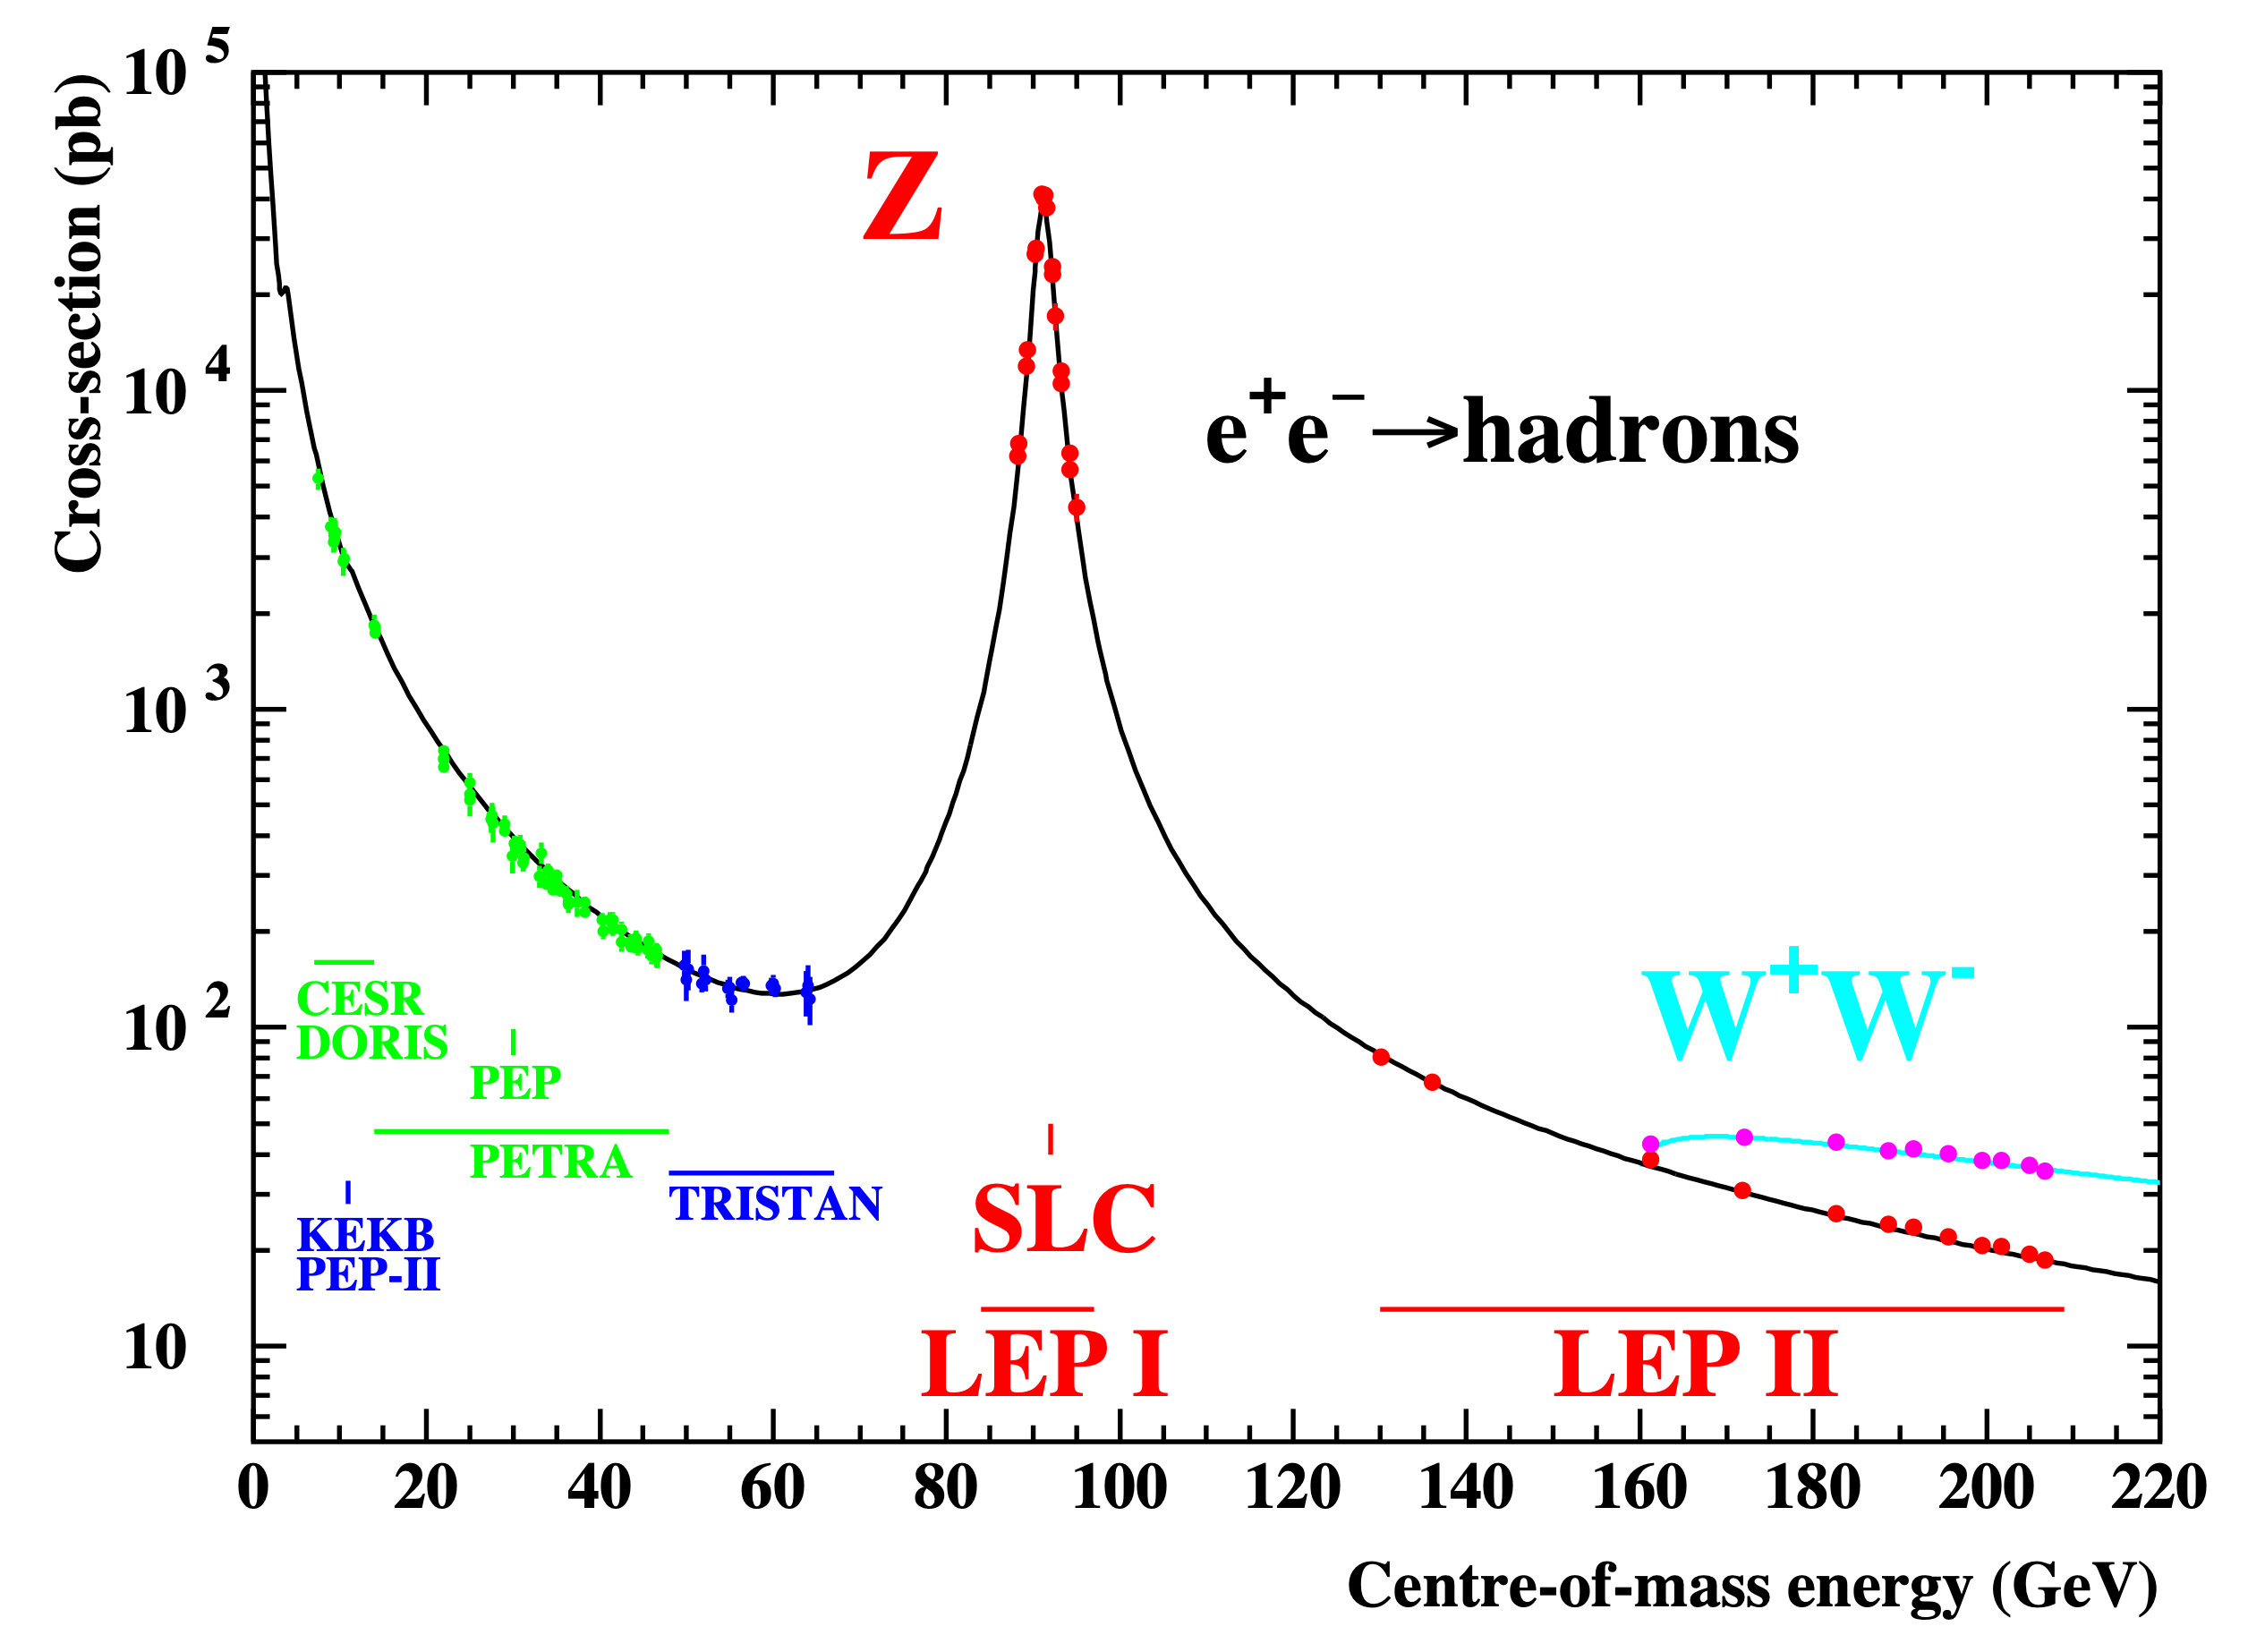
\includegraphics[width=0.8\textwidth]{figures/01-SM-02-QFT/eezpeak}
% 	\caption{Cross section for $e^+e^- \rightarrow$ hadron scattering as a function of $\sqrt{s}$ with a clear resonance at the $Z$ boson mass, reproduced from Ref.~\cite{ALEPH:2005ab}.}
% 	\label{fig:01_qft_interactions_eezpeak}
% \end{figure}


% \subsubsection{The classical limit and the Yukawa potential}

% It is important to check our QFT recovers classical physics in the appropriate limit.
% It will also be useful to translate the somewhat abstract idea of amplitudes to the familiar concepts of forces and potentials.
% We will do so by considering the nonrelativistic limit ($\abs{\vec{p}} \ll M$) of our above amplitudes and using the Born approximation relating the scattering amplitude between two particles to the potential between them $U(\vec{r})$:
% \begin{equation}
% 	\label{eq:01_qft_interactions_born}
% 	\mathcal M = \braket{\vec{p}_f|U(\vec{r})|\vec{p}_i} = -i \int U(\vec{r}) e^{i(\vec{p}_f - \vec{p}_i)\cdot\vec{r}} d^3r,
% \end{equation}
% where $\vec{r}$ is the displacement between the particles.

% First, let us consider what this potential would be classically.
% The static Klein-Gordon equation for a delta-function source:
% \begin{equation}
% 	\label{eq:01_qft_interactions_static_kg}
% 	(\nabla^2 - m^2) \phi(\vec{r}) = \delta^3(\vec{r}),
% \end{equation}
% can be found via the Fourier transform to be:
% \begin{equation}
% 	\label{eq:01_qft_interactions_static_kg_solution}
% 	\phi(\vec{r}) =  \cfrac{e^{-mr}}{4\pi r}.
% \end{equation}
% We can interpret this to be the profile of $\phi$ around a nucleon (the delta function source), and thus conversely the potential felt by another nucleon via the meson and the Yukawa interaction, under the assumption $M \gg m$.
% This is entirely analogous to gauge potential $A_0$ in electrostatics generated by a $\delta$-function source acting as the electric potential for a test charge.

% Going back to our amplitude for nucleon-antinucleon scattering, the $s$-channel diagram vanishes in the nonrelativistic limit (which essentially means it does not have a simple classical interpretation), while the $t$-channel diagram actually stays the same:
% \begin{equation}
% 	\label{eq:01_qft_interactions_na_scattering_nr}
% 	i \mathcal M = -(-ig)^2 \cdot \cfrac{1}{\abs{\vec{p}_f - \vec{p}_i}^2 - m^2}.
% \end{equation}
% Plugging this into the LHS of Eq.~\ref{eq:01_qft_interactions_born} and inverting the RHS integral gives us:
% \begin{equation}
% 	\label{eq:01_qft_interactions_yukawa_potential}
% 	U(\vec{r}) = -\cfrac{g^2}{4M^2} \cdot \cfrac{e^{-mr}}{4\pi r}.
% \end{equation}
% This is exactly the classical potential we found in Eq.~\ref{eq:01_qft_interactions_static_kg_solution}!
% It is weighted by the coupling constant $g$ and $M$ to get the correct dimensions, and with a minus sign telling us potential is attractive.

% Thus, we are able to reproduce Newtonian forces from the nonrelativisict limit of QFT.
% We also have the new interpretation of forces as simply manifestations of interactions in the Lagrangian, occurring through the exchange of virtual particles.

% This potential is called the \textit{Yukawa potential}, describing a force mediated by a massive boson.
% As expected, in the limit $m \rightarrow 0$, we recover the familiar $1/r$ Coulomb potential, which is mediated by the massless photon.
% We can check that we obtain the same potential for nucleon-nucleon scattering and, more generally, that all forces mediated by scalars are attractive.
% In fact, this is true for spin-2 particles as well, which is why gravity is universally attractive!
% On the other hand, forces mediated by spin-1 particles, such as EM, can be either attractive or repulsive, with the charges of the particles involved determining the sign of each diagram.
% See e.g. Zee QFT~\cite{Zee:2003mt} Chapter I.5 for a useful discussion.

% \subsubsection{Fourth-order diagrams and loops}

% So far, we have only considered \textit{tree-level} diagrams, the simplest to calculate.
% This is in contrast to diagrams with \textit{loops}, which can occur at higher order in perturbation theory.
% For example, at fourth-order we can have diagrams like those in Figure~\ref{fig:01_qft_interactions_feynman_loops} for nucleon scattering. 

% Such diagrams contribute integrals over the loop momentum $k$ to the matrix element, which can notoriously diverge.
% To deal with this requires a process called \textit{renormalization}, which, briefly, involves defining a cut-off energy scale $\Lambda$ for these integrals, beyond which we claim the theory is invalid.
% Experimentally, the main consequence is that physical parameters like the mass of particles and coupling constants in fact depend on the energy scale at which they are measured!

% \begin{figure}[ht]
% 	\centering
% 	\captionsetup{justification=centering}
% 	\begin{tikzpicture}
% 		\begin{feynman}
% 			\vertex (a);
% 			\vertex [below=1cm of a] (c);
% 			\vertex [below=1.2cm of c] (d);
% 			\vertex [below=1cm of d] (b);
% 			\vertex [above left=of a] (i1);
% 			\vertex [below left=of b] (i2);
% 			\vertex [above right=of a] (f1);
% 			\vertex [below right=of b] (f2);
% 			\diagram* {
% 				(a) -- [scalar, edge label={\footnotesize\(k_1\)}] (c),
% 				(d) -- [scalar, edge label={\footnotesize\(k_3\)}] (b),
% 				(i1) -- [fermion, edge label'={\footnotesize\(q_{i1}\)}] (a),
% 				(i2) -- [fermion, edge label={\footnotesize\(q_{i2}\)}] (b),
% 				(a) -- [fermion, edge label'={\footnotesize\(q_{f1}\)}] (f1),
% 				(b) -- [fermion, edge label={\footnotesize\(q_{f2}\)}] (f2),
% 				(c) -- [fermion, half left, edge label'={\footnotesize\(k_2\)}] (d),
% 				(d) -- [fermion, half left] (c),
% 			};
% 		\end{feynman}
% 	\end{tikzpicture}
% 	\caption{An example of a higher-order scattering diagram with a ``loop''.}
% 	\label{fig:01_qft_interactions_feynman_loops}
% \end{figure}

% \subsection{Decay rates and cross sections}
% \label{sec:01_qft_interactions_decay}

% In this section, we translate our S-matrix elements to physical observables: cross sections and decay rates.


% \subsubsection{Cross section}

% Classically for a scattering experiment, the number of particles scattered $N$ is related to the cross sectional area $\sigma$ as:
% \begin{equation}
% 	\label{eq:01_qft_interactions_cross_section_classical}
% 	N = \sigma T \Phi,
% \end{equation}
% where $T$ is the total time and $\Phi$ is the flux of incoming particles (number of incoming particles per unit area and unit time).
% In QM, we define the cross section $\sigma$ similarly, but in terms of the probability of scattering $P$ instead of $N$:
% \begin{equation}
% 	\label{eq:01_qft_interactions_cross_section_qm}
% 	\sigma = \frac{P}{\Phi T}.
% \end{equation}
% This is a more abstract quantity in QM, but it still has units of area.
% The number of scattering events $N$ is related to $\sigma$ by a factor we call the \textit{luminosity} $L$:
% \begin{equation}
% 	\label{eq:01_qft_interactions_cross_section_luminosity}
% 	N = \sigma L.
% \end{equation}
% Here, we simply consider this the definition of luminosity, but for a collider, for example, it can be derived from the properties of the input particle beams  (as will be discussed in Part~\ref{part:epp}).
% Often, we are interested in the \textit{differential cross section} $d\sigma$ with respect to kinematic variables like the solid angle $\Omega$ or energy, so we write:
% \begin{equation}
% 	\label{eq:01_qft_interactions_cross_section_differential}
% 	d\sigma = \frac{dP}{\Phi T}.
% \end{equation}

% As in QM, this probability $P$ is proportional to the square of the amplitude $|\braket{f|S|i}|^2$:
% \begin{equation}
% 	\label{eq:01_qft_interactions_cross_section_probability}
% 	dP = \frac{\abs{\braket{f|S|i}}^2}{\braket{f|f}\braket{i|i}}\, d\Pi,
% \end{equation}
% where $\braket{f|f}$ and $\braket{i|i}$ are the normalization factors for the final and initial states (they are not equal to $1$ as discussed in Section~\ref{sec:01_qft_quantization_propagators}), and $d\Pi$ is the differential region of final state momenta.

% For the case of two incoming particles (which is what is most relevant for this dissertation), we can put all of this together to obtain the relation between differential cross section and the matrix element $\mathcal M$:
% \begin{equation}
% 	\label{eq:01_qft_interactions_cross_section_matrix_element}
% 	d\sigma = \frac{1}{(2E_1)(2E_2)\abs{\vec{v}_1 - \vec{v}_2}} \abs{\mathcal M}^2 d\Pi_{\mathrm{LIPS}},
% \end{equation}
% where $E_1$ and $E_2$ are the energies of the incoming particles, $\vec{v}_1$ and $\vec{v}_2$ are their velocities, and $d\Pi_{\mathrm{LIPS}}$ is called the Lorentz-invariant phase space of the final state momenta:
% \begin{equation}
% 	\label{eq:01_qft_interactions_cross_section_lips}
% 	d\Pi_{\mathrm{LIPS}} = (2\pi)^4 \delta^{(4)}(\Sigma p) \prod_{\mathrm{final\ states}\ j} \frac{d^3p_j}{(2\pi)^3} \frac{1}{2E_j}
% \end{equation}

% For the case of $2 \rightarrow 2$ scattering, in the COM frame, this simplifies considerably:
% \begin{equation}
% 	\label{eq:01_qft_interactions_cross_section_com}
% 	\bigg(\frac{d\sigma}{d\Omega}\bigg)_{\mathrm{CM}} = \frac{1}{64\pi^2E_{\mathrm{CM}}^2}\, \frac{\abs{\vec{p}_f}}{\abs{\vec{p}_i}} \abs{\mathcal M}^2 \theta(E_{\mathrm{CM}} - m_3 - m_4),
% \end{equation}
% and even more so when the all four masses are equal:
% \begin{equation}
% 	\label{eq:01_qft_interactions_cross_section_com_equal_mass}
% 	\bigg(\frac{d\sigma}{d\Omega}\bigg)_{\mathrm{CM}} = \frac{1}{64\pi^2E_{\mathrm{CM}}^2}\, \abs{\mathcal M}^2.
% \end{equation}

% For nucleon-nucleon scattering in the COM frame, for example, we have (at tree level):
% \begin{equation}
% 	\label{eq:01_qft_interactions_nn_scattering_cross_section}
% 	\begin{split}
% 		\bigg(\frac{d\sigma(\theta)}{d\Omega}\bigg)_{\mathrm{CM}} &= \frac{g^4}{64\pi (2E)^2} \left(\frac{1}{t - m^2} + \frac{1}{u - m^2}\right)^2 \\
% 		&= \frac{g^4}{64\pi (2E)^2} \left[\frac{1}{2p^2(1 - \cos\theta) - m^2} + \frac{1}{2p^2(1 + \cos\theta) - m^2}\right]^2,
% 	\end{split}
% \end{equation}
% where we used the expressions for $t$ and $u$ for a collision along the z-axis from Eq.~\ref{eq:01_qft_interactions_mandelstam_com}.

% \subsubsection{Decay rate}

% The other type of process we are interested in are decays.
% The decay rate $\Gamma$ is simply the probability of decay per unit time:
% \begin{equation}
% 	\label{eq:01_qft_interactions_decay_rate}
% 	\Gamma =  \frac{P}{T}.
% \end{equation}
% Using our expression for $P$ from above and simplifying, we find:
% \begin{equation}
% 	\label{eq:01_qft_interactions_differential_decay_rate}
% 	d\Gamma = \frac{1}{2m} \abs{\mathcal M}^2 d\Pi_{\mathrm{LIPS}},
% \end{equation}
% in the rest frame of the decaying particle, where $m$ is its mass.
% If multiple decays of the same particle are possible, we sum over the final states in the phase space integral.
% The total $\Gamma$ is then called the \textit{width} of the particle, and $1/\Gamma \equiv \tau$ is its half-life.

% For our simple meson decay $\phi \rightarrow \psi^\dagger\psi$, we have at tree level:
% \begin{equation}
% 	\label{eq:01_qft_interactions_decay_rate_meson_decay}
% 	d\Gamma = \frac{g^2}{2m} d\Pi_{\mathrm{LIPS}} \quad \Rightarrow \quad \Gamma = \frac{g^2}{32\pi m} \left(1 - \frac{4M^2}{m^2}\right)^{1/2},
% \end{equation}
% where we performed the integral over $d\Pi_{\mathrm{LIPS}}$ (see Ref.~\cite{XianyuPSSolutions} 4.2).
% This is in fact not too far off the expression for the decay width of the Higgs boson to fermions.
% What we are missing of course is that fermions are spin-$\cnicefrac{1}{2}$ particles, and we need to sum over their spin states.
% We will derive the correct expression (at tree level) in the next section.

% \section{Spinor field theory}
% \label{sec:01_qft_spinors}

% \begin{center}
% 	\centering
% 	\noindent
% 	\textit{...anything that comes back to itself with a minus sign after a 2$\pi$ rotation is always going to be a little strange.} --- David Tong~\cite{TongSM}
% \end{center}

% So far, we have focused on scalar fields, which live in the trivial representation of the Lorentz group and correspond to spin-$0$ bosons.
% In this section, we discuss the field theory for spin-$\frac{1}{2}$ particles, or fermions, which constitute all matter in the universe.
% % As discussed in Chapter~\ref{sec:01_symmetries_poincare}, all known elementary fermions are associated with \textit{Dirac spinor} fields, which transform under the $(\cnicefrac{1}{2},0) \oplus (0,\cnicefrac{1}{2})$ representation of the Lorentz group.
% % We describe the EOM governing free spinor fields, known as the Dirac equation, in Section~\ref{sec:01_qft_spinors_dirac}.
% % \TODO{We then...}
% % We then quantize the free spinor field in Section~\ref{sec:01_qft_spinors_quantization} and finally discuss Feynman rules for an interacting spinor theory in Section~\ref{sec:01_qft_spinors_feynman}.

% \subsection{The Dirac equation}
% \label{sec:01_qft_spinors_dirac}

% % \subsubsection{Historical development}

% Like the Klein-Gordon equation, the Dirac equation was also an attempt at a relativistic version of the Schrödinger equation.
% Before the development of QFT, the quantized KG equation was thought to produce negative probabilities due to its second derivative in time.\footnote{We now understand that the KG equation describes perfectly good scalar quantum fields, where the field-theoretic analog of the probability density is in fact the conserved charge of Eq.~\ref{eq:01_qft_quantization_complex_charge}, which is allowed to be negative.}
% Dirac thus sought a relativistic \textit{first-order} differential equation in space and time.

% Legend has it he was staring into a fire in Cambridge when he came up with an equation of the form
% \begin{equation}
% 	\label{eq:01_qft_spinors_dirac}
% 	(i\gamma^\mu \partial_\mu - m)\psi = 0,
% \end{equation}
% where $\gamma^\mu$ are constants that will be defined in a moment, and $\psi$ is a complex field.
% It is difficult to make this equation Lorentz covariant; indeed, it is impossible if $\psi$ is a scalar and each $\gamma^\mu$ is simply a number.\footnote{Or even two- or three-dimensional.}
% Dirac's brilliant insight, however, was that it \textit{can} be covariant if $\gamma_\mu$ are $4\times 4$ complex matrices and $\psi$ a four component field.

% The key is that $\gamma^\mu\partial_\mu$ is essentially the ``square-root'' of the d'Alembertian $\Box$ from the KG-equation:
% \begin{equation}
% 	\label{eq:01_qft_spinors_dirac_wave}
% 	\gamma^\mu \partial_\mu \gamma^\nu \partial_\nu = \Box = \partial_\mu \partial^\mu,
% \end{equation}
% if (and only if) $\gamma^\mu$ and $\gamma^\nu$ satisfy the \textit{Clifford algebra}:
% \begin{equation}
% 	\label{eq:01_qft_spinors_clifford_algebra}
% 	\{\gamma^\mu, \gamma^\nu\} = 2\eta^{\mu\nu},
% \end{equation}
% where $\{A, B\} = AB + BA$ is the anticommutator.
% Dirac found this is possible with $4\times 4$ matrices such as
% % Equation~\ref{eq:01_qft_spinors_clifford_algebra} defines \textit{Clifford algebra}, which has irreps only of dimension $4$, such as
% \begin{equation}
% 	\label{eq:01_qft_spinors_gamma_matrices_weyl_basis}
% 	% \setlength{\arraycolsep}{8pt}
% 	\gamma^0 = \begin{pmatrix} 0 & \identity \\ \identity & 0 \end{pmatrix}, \quad 
% 	\gamma^i = \begin{pmatrix} 0 & \sigma^i \\ -\sigma^i & 0 \end{pmatrix},
% \end{equation}
% where $\sigma^i$ are the Pauli matrices (Chapter~\ref{sec:01_symmetries_so3}).
% These are called the \textit{gamma}, or \textit{Dirac}, matrices, and plugging them into Eq.~\ref{eq:01_qft_spinors_dirac} yields the \textit{Dirac equation}, which can be written even more compactly by defining $\slashed{\partial} \equiv \gamma^\mu \partial_\mu$:
% \begin{equation}
% 	\label{eq:01_qft_spinors_dirac_slash}
% 	(i\slashed{\partial} - m)\psi = 0.
% \end{equation}

% This equation is considered one of the most significant breakthroughs in theoretical physics, ``on par with the works of Newton, Maxwell, and Einstein before him''~\cite{hey2003new}.
% The insights that followed, as we will outline in this section, provided a theoretical basis for fermion spin, implied the existence of antiparticles, and overall were foundational to the development of the SM.\footnote{These insights were so unexpected that Dirac thought ``his equation was more intelligent than its author''~\cite{brown1983birth}.}

% \subsection{Spinors}
% \label{sec:01_qft_spinors_spinors}

% Before discussing solutions and quantization of the Dirac equation, let us examine what kind of object $\psi$ is.
% A related property of the Clifford algebra is that
% \begin{equation}
% 	\label{eq:01_qft_spinors_gamma_lorentz_generators}
% 	\Sigma_{\mu\nu} \equiv \frac{i}{4}[\gamma^\mu, \gamma^\nu]
% \end{equation}
% satisfies the Lorentz algebra (Eq.~\ref{eq:01_poincare_algebra_mmunu}).
% This means $\Sigma_{\mu\nu}$ are generators of Lorentz transformations
% \begin{equation}
% 	\label{eq:01_qft_spinors_spinor_lorentz_transformation}
% 	S[\Lambda] = e^{\frac{1}{2}\omega^{\mu\nu}\Sigma_{\mu\nu}}, 
% \end{equation}
% where $\Lambda$ is a Lorentz transformation with parameters $\omega^{\mu\nu}$, and $S[\Lambda]$ is a particular 4D representation.

% It can be shown\footnote{See e.g. Ref.~\cite{LiuRQFT} Lecture 14.} that the Dirac equation is only Lorentz covariant if the components of $\psi$, $\psi_\alpha$, transform under this exact representation:
% \begin{equation}
% 	\label{eq:01_qft_spinors_spinor_transformation}
% 	\psi_\alpha \rightarrow \psi'_\alpha = S[\Lambda]^\beta_{\ \alpha} \psi_\beta.
% \end{equation}
% It is important to note here that $S[\Lambda]$ is acting on the $\psi$ components --- also called the spinor indices -- and not on the spacetime coordinates $x^\mu$, which transform under the vector representation (Eq.~\ref{eq:01_lorentz_generators}).
% Explicitly, including the spacetime coordinates, $\psi(x)$ transforms as:
% \begin{equation}
% 	\label{eq:01_qft_spinors_spinor_transformation_x}
% 	\psi_\alpha(x) \rightarrow \psi'_\alpha(x') = S[\Lambda]^\beta_{\ \alpha} \psi_\beta(\Lambda^{-1}x),
% \end{equation}
% where both $S[\Lambda]$ and $\Lambda$ share the same transformation parameters $\omega^{\mu\nu}$ and thus correspond to the same Lorentz transformation.\footnote{$x' = \Lambda^{-1}x$ as this is an \textit{active} transformation, in which the field is shifted.}

% \subsubsection{Dirac and Weyl spinors}

% What is this representation?
% Let's look at the rotation and boost generators individually:
% \begin{equation}
% 	\label{eq:01_qft_spinors_spinor_generators}
% 	\Sigma_{0i} = \frac{i}{2} \begin{pmatrix} -\sigma^i & 0 \\ 0 & \sigma^i \end{pmatrix}, \quad
% 	\Sigma_{ij} = \frac{1}{2} \epsilon_{ijk} \begin{pmatrix} \sigma^k & 0 \\ 0 & \sigma^k \end{pmatrix}.
% \end{equation}
% Comparing this with Eqs.~\ref{eq:01_lorentz_irreps_weyl_left} and~\ref{eq:01_lorentz_irreps_weyl_right}, we see that the top left and bottom right blocks are exactly the left- and right-handed Weyl spinor irreps of the generators.
% The handedness of a spinor is called its \textit{chirality}, and its physical significance will be discussed in a moment.
% Thus, we identify $S[\Lambda]$ with the $(\cnicefrac{1}{2},0) \oplus (0,\cnicefrac{1}{2})$, or Dirac spinor, representation.

% This also means that, in this basis of the gamma matrices (called the \textit{Weyl}, or \textit{chiral}, basis), the Dirac spinor $\psi$ can be decomposed into two Weyl spinors:
% \begin{equation}
% 	\label{eq:01_qft_spinors_spinor_decomposition}
% 	\psi = \begin{pmatrix} \psi_L \\ \psi_R \end{pmatrix},
% \end{equation}
% which transform under their respective representations.
% The two components can be isolated if we consider a fifth gamma matrix:
% \begin{equation}
% 	\label{eq:01_qft_spinors_gamma_five}
% 	\gamma^5 = i\gamma^0\gamma^1\gamma^2\gamma^3 = \begin{pmatrix} -\identity & 0 \\ 0 & \identity \end{pmatrix}.
% \end{equation}
% $\gamma^5$ is similar to our main four matrices in that $\{\gamma^5, \gamma^\mu\} = 0$ and $(\gamma^5)^2 = \identity$.
% Importantly, we see from its form in the Chiral basis that projection operators $P_L$ and $P_R$ can be defined as:
% \begin{equation}
% 	\label{eq:01_qft_spinors_chiral_projection}
% 	P_L = \frac{1 - \gamma^5}{2}, \quad P_R = \frac{1 + \gamma^5}{2},
% \end{equation}
% which satisfy the projection property $P_{L/R}^2 = P_{L/R}$ and project out the left- and right-handed components of a Dirac spinor:
% \begin{equation}
% 	\label{eq:01_qft_spinors_chiral_projection_action}
% 	P_{L} \begin{pmatrix} \psi_L \\ \psi_R \end{pmatrix} = \begin{pmatrix} \psi_L \\ 0 \end{pmatrix}, \quad P_{R} \begin{pmatrix} \psi_L \\ \psi_R \end{pmatrix} = \begin{pmatrix} 0 \\ \psi_R \end{pmatrix}.
% \end{equation}
% Note that while the specific form depends on the basis, the definitions in Eq.~\ref{eq:01_qft_spinors_chiral_projection} are basis-independent and can be considered to define chirality.

% \subsubsection{Chirality}

% The two Weyl spinor representations are related by a complex conjugation, meaning $\psi_L^*$ is a right-handed Weyl spinor, and vice versa.
% For a complex scalar field, we interpreted the conjugate as the antiparticle.
% The same interpretation applies here; hence, if a left-handed spinor describes a particle, its antiparticle is described by its conjugate, right-handed spinor.

% The Dirac equation can be rewritten in the Weyl basis as two coupled equations of the Weyl spinors.
% Let us define $\sigma^\mu = (\identity, \vec{\sigma})$ and $\bar{\sigma}^\mu = (\identity, -\vec{\sigma})$, so that
% \begin{equation}
% 	\label{eq:01_qft_spinors_dirac_weyl}
% 	(i\gamma^\mu\partial_\mu - m)\psi = 
% 	\begin{pmatrix} 
% 		-m & i\sigma^\mu\partial_\mu \\ i\bar{\sigma}^\mu\partial_\mu & -m 
% 	\end{pmatrix}
% 	\begin{pmatrix} \psi_L \\ \psi_R \end{pmatrix} = 0.
% \end{equation}
% Hence, we see the mass term couples the left- and right-handed components. 
% This is why all massive fermions must exist in pairs of particles and antiparticles.
% An important special case, however, is for a neutral \textit{Majorana} fermion, where $\psi$ equals its charge conjugate $\psi^c$ (to be defined below). 
% Such a particle is its own antiparticle and can have a left-handed- or right-handed-only mass term.
% As discussed in Chapter~\ref{sec:01_symmetries_poincare}, the only Majorana candidate in the SM is the right-handed neutrino.

% For $m = 0$, the Dirac equation decouples and leaves us with the \textit{Weyl equations} describing massless fermions:
% \begin{equation}
% 	\label{eq:01_qft_spinors_weyl}
% 	i\sigma^\mu\partial_\mu \psi_R= 0, \quad i\bar{\sigma}^\mu\partial_\mu \psi_L = 0.
% \end{equation}
% In Fourier space, these are:
% \begin{equation}
% 	\label{eq:01_qft_spinors_weyl_fourier}
% 	\begin{split}
% 		\sigma^\mu p_\mu \psi_R = (E - \vec{\sigma}\cdot\vec{p})\psi_R = 0 \quad \Rightarrow \quad  \frac{\vec{\sigma}\cdot\vec{p}}{\abs{\vec{p}}}\, \psi_R = +\psi_R, \\
% 		\bar{\sigma}^\mu p_\mu \psi_L = (E + \vec{\sigma}\cdot\vec{p})\psi_L = 0 \quad \Rightarrow \quad \frac{\vec{\sigma}\cdot\vec{p}}{\abs{\vec{p}}}\, \psi_L = -\psi_L,
% 	\end{split}
% \end{equation}
% where we used $E = \abs{\vec{p}}$ for massless particles.
% You may recall $\frac{\vec{\sigma}\cdot\vec{p}}{\abs{\vec{p}}}$ is the helicity operator, projecting the particle spin along its momentum.
% Thus, in the massless limit, we see that the left- and right-handed Weyl spinors are the $+1$ and $-1$ helicity eigenstates, respectively.

% This is not the case for massive particles, as helicity is no longer Lorentz invariant: one can always boost into a frame where the momentum is inverted while the spin remains the same, changing the sign of the helicity.
% Chirality is thus a more abstract concept for massive particles, related only to how they transform under Lorentz transformations.

% Theories not symmetric under exchange of left- and right-handed components are called \textit{chiral}, and symmetric theories \textit{vector}.
% QED and QCD are both vector theories, but weak interactions are, surprisingly, chiral.
% This necessarily means it violates parity and charge conjugation symmetries ($P$ and $C$), which we will discuss soon in Section~\ref{sec:01_qft_spinors_cpt}.


% \subsection{The Dirac Lagrangian}
% \label{sec:01_qft_spinors_lagrangian}

% Recall that to quantize the scalar theory, we first needed the Lagrangian and the classical solutions of the K-G equation, to then obtain Hamiltonian and canonical fields and Poisson brackets before finally promoting them to quantum commutatation relations.
% We will proceed in similar (though condensed) fashion for the spinor theory, and first derive the Lagrangian corresponding to the Dirac equation.

% Since we are no longer dealing with trivial representation of the Lorentz group, we have to be more careful with the types of terms we put into the Lagrangian; it must be composed of good Lorentz-invariant objects.
% % The action is Lorentz invariant, so the Lagrangian must be composed of good Lorentz-covariant objects.
% A first guess at a Lorentz scalar formed of spinors may be $\psi^\dagger\psi$.
% This is indeed a scalar, but it is \textit{not} Lorentz invariant:
% $\psi$ and $\psi^\dagger$ transform as $\psi\rightarrow S[\Lambda]\psi$, $\psi^\dagger\rightarrow \psi^\dagger S[\Lambda]^\dagger$ and, hence
% \begin{equation}
% 	\label{eq:01_qft_spinors_lagrangian_scalar_wrong}
% 	\psi^\dagger\psi \rightarrow \psi^\dagger S[\Lambda]^\dagger S[\Lambda]\psi. % \neq \psi^\dagger\psi.
% \end{equation}
% However, recall from Chapter~\ref{sec:01_symmetries_poincare} that (finite-dimensional) representations of Lorentz transformations are not unitary.
% (We can see this as well from the fact that the generators of $S[\Lambda]$ in Eq.~\ref{eq:01_qft_spinors_spinor_generators} are not anti-Hermitian.)
% Thus, $S[\Lambda]^\dagger S[\Lambda] \neq 1$ in general and $\psi^\dagger\psi$ is not a Lorentz scalar.

% Instead, with a bit of matrix algebra\footnote{See e.g. Schwartz~\cite{Schwartz:2014sze} Chapter 10.3}, one can show that
% \begin{equation}
% 	\label{eq:01_qft_spinors_gamma0_inverse}
% 	\gamma^0 S[\Lambda] \gamma^0 = (S[\Lambda]^{-1})^\dagger,
% \end{equation}
% and hence
% \begin{equation}
% 	\label{eq:01_qft_spinors_lagrangian_scalar}
% 	\psi^\dagger\gamma^0\psi \rightarrow \psi^\dagger S[\Lambda]^\dagger \gamma^0 S[\Lambda]\psi = \psi^\dagger\gamma^0 S[\Lambda]^{-1} S[\Lambda]\psi = \psi^\dagger\gamma^0\psi
% \end{equation}
% \textit{is} a Lorentz scalar.
% Thus, we define $\bar\psi \equiv \psi^\dagger\gamma^0$ as the ``natural'' conjugate to $\psi$, and end up with a nice Lorentz scalar $\bar\psi \psi$ for our Lagrangian.

% Similarly, one can show that $\bar\psi\gamma^\mu\psi$ transforms as a Lorentz $4$-vector and, hence, contracting it with $\partial_\mu$ as $\bar\psi\gamma^\mu\partial_\mu\psi$ yields another scalar.
% These two terms, which are analogous to the mass and derivative terms a free complex scalar field (Eq.~\ref{eq:01_qft_symmetries_complex_lagrangian}), are enough to build the Dirac lagrangian:
% \begin{equation}
% 	\label{eq:01_qft_spinors_lagrangian}
% 	\mathcal{L} = i\bar\psi\gamma^\mu\partial_\mu\psi - m\bar\psi\psi = \bar\psi(i\slashed{\partial} - m)\psi.
% \end{equation}
% One can check that the EL equations reproduce the Dirac equation for $\psi$ and $\bar\psi$.

% \subsubsection{The U(1) conserved current}

% As with the complex scalar field, observe that the Dirac Lagrangian is invariant under global \UU[1] symmetry $\psi \rightarrow e^{i\alpha}\psi$.
% Using Noether's theorem, we can derive the conserved current and charge associated with this symmetry:
% \begin{equation}
% 	\label{eq:01_qft_spinors_lagrangian_current}
% 	j^\mu = \bar\psi\gamma^\mu\psi, \quad Q = \int d^3x\, j^0 = \int d^3x\, \psi^\dagger\psi.
% \end{equation}
% As for the complex scalar field, these represent the electromagnetic $4$-current and charge, respectively --- a connection we will explore further in Section~\ref{sec:01_qft_gt_maxwell}.


% \subsection{Quantizing the Dirac field}
% \label{sec:01_qft_spinors_quantization}

% \subsubsection{Solutions to the Dirac equation}

% Before quantizing, we first need the classical solutions to the Dirac equation.
% Multiplying both sides of it by $-(i\gamma^\mu\partial_\mu + m)$ gives us:
% \begin{equation}
% 	\label{eq:01_qft_spinors_dirac_squared}
% 	-(i\gamma^\mu\partial_\mu + m)(i\gamma^\nu\partial_\nu - m)\psi = (\Box - m^2)\psi = 0,
% \end{equation}
% which means each component of $\psi$ individually satisfies the KG-equation.
% Thus, we can assume similar plane wave solutions:
% \begin{equation}
% 	\label{eq:01_qft_spinors_dirac_solution}
% 	\psi(x) = \int \frac{d^3p}{(2\pi)^3} \, u(p) e^{-ip\cdot x} + v(p) e^{ip\cdot x},
% \end{equation}
% where $u(p)$ and $v(p)$ are now spinors, and again we have positive and negative frequency solutions that correspond to particles and antiparticles, respectively, after quantization.

% One can check using Fourier space, as we did for the Weyl equations, that
% \begin{equation}
% 	\label{eq:01_qft_spinors_dirac_solution_up}
% 	u(p) = \begin{pmatrix} \sqrt{p \cdot \sigma}\, \xi \\ \sqrt{p \cdot \bar\sigma}\, \xi \end{pmatrix}, \quad
% 	v(p) = \begin{pmatrix} \sqrt{p \cdot \sigma}\, \eta \\ -\sqrt{p \cdot \bar\sigma}\, \eta \end{pmatrix}
% \end{equation}
% are general solutions to the Dirac equation, where $\xi$ and $\eta$ are the familiar two-component spinors from QM for spin-$\cnicefrac{1}{2}$ particles (although technically they do not have this interpretation before quantization).
% As is conventional, we will use a basis of $\sigma_z$ eigenstates $\xi_1 = \eta_1 = (1, 0)^T$ and $\xi_2 = \eta_2 = (0, 1)^T$, corresponding to spin-up and spin-down, respectively.
% % , with eigenvalues $+1$ and $-1$, respectively.

% For example, in the rest frame $p_\mu = (m, 0, 0, 0)$, we have:
% \begin{equation}
% 	\label{eq:01_qft_spinors_dirac_solution_rest}
% 	u(p)_1 = \sqrt{m} \begin{pmatrix} 1 \\ 0 \\ 1 \\ 0 \end{pmatrix}, \,
% 	u(p)_2 = \sqrt{m} \begin{pmatrix} 0 \\ 1 \\ 0 \\ 1 \end{pmatrix}, \,
% 	v(p)_1 = \sqrt{m} \begin{pmatrix} 1 \\ 0 \\ -1 \\ 0 \end{pmatrix}, \,
% 	v(p)_2 = \sqrt{m} \begin{pmatrix} 0 \\ 1 \\ 0 \\ -1 \end{pmatrix}.
% \end{equation}
% More generally, we can always orient a particle's 3-momentum along the $z$-axis, in which case:
% \begin{equation}
% 	\label{eq:01_qft_spinors_dirac_solution_momentum}
% \resizebox{\textwidth}{!}{$
% 	u(p)_1 = \begin{pmatrix} \sqrt{E - p_z} \\ 0 \\ \sqrt{E + p_z} \\ 0 \end{pmatrix}, \quad
% 	u(p)_2 = \begin{pmatrix} 0 \\ \sqrt{E - p_z} \\ 0 \\ \sqrt{E + p_z} \end{pmatrix} \quad
% 	v(p)_1 = \begin{pmatrix} \sqrt{E + p_z} \\ 0 \\ -\sqrt{E - p_z} \\ 0 \end{pmatrix}, \quad
% 	v(p)_2 = \begin{pmatrix} 0 \\ \sqrt{E + p_z} \\ 0 \\ -\sqrt{E - p_z} \end{pmatrix}.
% $}
% \end{equation}

% \subsubsection{Quantization}

% Now that we have a sensible Lagrangian and the classical solutions to the Dirac equation, the remaining steps to quantization follow closely that for our complex scalar field in Section~\ref{sec:01_qft_quantization_complex}, but with two notable differences.
% The first is that we now must sum over the two spin components of $u_s(p)$ and $v_s(p)$, in addition to integrating over the momentum:
% \begin{equation}
% 	\label{eq:01_qft_spinors_quantization}
% 	\begin{split}
% 		\psi(x) &= \sum_{s = 1, 2} \int \frac{d^3p}{(2\pi)^3} \left[\hat b^s_{\vec{p}}\, u_s(p) e^{-ip\cdot x} + c^{s\dagger}_{\vec{p}}\, v_s(p) e^{ip\cdot x}\right], \\
% 		\bar\psi(x) &= \sum_{s = 1, 2} \int \frac{d^3p}{(2\pi)^3} \left[\hat b^{s\dagger}_{\vec{p}}\, \bar{u}_s(p) e^{ip\cdot x} + \hat c^s_{\vec{p}}\,  \bar{v}_s(p) e^{-ip\cdot x}\right].
% 	\end{split}
% \end{equation}
% As before, we have positive and negative frequency solutions, with the $b/b^\dagger$ and $c/c^\dagger$ operators associated with particles of the same mass and opposite charge.

% For spinors, we find that the $\hat b^{s\dagger} \ket{0}$ and $\hat c^{s\dagger} \ket{0}$ also have opposite spins, i.e. for the $z$-axis angular momentum operator $J_z$ (which can be derived through Noether's theorem as we did for the momentum operator in Section~\ref{sec:01_qft_classical_symmetries}):
% \begin{equation}
% 	\label{eq:01_qft_spinors_spin_z}
% 	J_z\, \hat b^{s\dagger} \ket{0} = \pm\frac{1}{2} \hat b^{s\dagger} \ket{0}, \quad J_z\, \hat c^{s\dagger}\ket{0} = \mp \frac{1}{2} \hat c^{s\dagger}\ket{0}.
% \end{equation}
% By convention, we take $b^{s\dagger}$ and $b^s$ to be the creation and annihilation operators for the electron, and $c^{s\dagger}$ and $c^s$ for its antiparticle, the positron.
% Thus, $\bar\psi_s(x)\ket{0}$ corresponds to an electron at $x$ with spin state $s$, and $\psi_s(x)\ket{0}$ to a positron at $x$ with the opposite spin state to $s$.

% Through his equation, Dirac was the first to predict the existence of antimatter in 1930~\cite{Dirac:1930ek} (although he initially thought the electron's antiparticle was the proton).
% This prediction was soon confirmed by the discovery of a particle with the same mass as the electron but opposite charge by Carl Anderson in a bubble chamber in 1932~\cite{Anderson:1932zz}.
% Both were awarded the Nobel prize.

% % made shocking prediction, and they were discovered.
% % particles created by b have same mass as by a, but opposite charge and spin (?).

% \subsubsection{The spin-statistics connection}

% The second, extremely important difference from scalar quantization is that, because spinors are spin-$\frac{1}{2}$ particles, they must obey \textit{anticommutation relations}:
% \begin{equation}
% 	\label{eq:01_qft_spinors_anticommutation}
% 	\begin{split}
% 		\{\psi_\alpha(x), \psi_\beta(y)\} =& \,\{\bar\psi_\alpha(x), \bar\psi_\beta(y)\} = 0, \\
% 		\{\psi_\alpha(x), \bar\psi_\beta(y)\} &= \delta_{\alpha\beta}\delta^3(\vec{x} - \vec{y}),
% 	\end{split}
% \end{equation}
% which also means the creation and annihilation operators satisfy:
% \begin{equation}
% 	\label{eq:01_qft_spinors_anticommutation_operators}
% 	% \{a_s(p), a_{r}^\dagger(q)\} = \{b_s(p), b_{r}^\dagger(q)\} = (2\pi)^3\delta^3(\vec{p} - \vec{q})\delta_{sr}.
% 	\{\hat b^{s}_{\vec{p}}, \hat b^{r\dagger}_{\vec{q}}\} = \{\hat c^{s}_{\vec{p}}, \hat c^{r\dagger}_{\vec{q}}\} = (2\pi)^3\delta^3(\vec{p} - \vec{q})\delta_{sr}.
% \end{equation}
% Thus, unlike bosons, exchanging two particles yields a minus sign: $\hat b^{r\dagger}_{\vec{p}_1} \hat b^{s\dagger}_{\vec{p}_1} \ket{0} = -\hat b^{s\dagger}_{\vec{p}_2} \hat b^{r\dagger}_{\vec{p}_1} \ket{0}$, confirming that spinors obey Fermi-Dirac statistics and obey the Paul-Exclusion principle.

% Were we to try and impose our earlier commutation relations for spinors (or indeed, any half-integer-spin field), we would run into several issues.
% These include the time-ordered product in the $S$-matrix not being Lorentz invariant, and antiparticles contributing arbitrarily negative energies, making the theory unstable.
% They are all related to the deep connection between spin and statistics: the requirement of Lorentz invariance, stability, and causality in a QFT necessitates that half-integer-spin particles obey Fermi-Dirac, and integer-spin particles Bose-Einstein statistics.\footnote{For more detailed discussion, see e.g. Peskin and Schroeder~\cite{Peskin:1995ev} Chapter 3.5 and Schwartz~\cite{Schwartz:2014sze} Chapter 12.}


% \subsection{Interactions and Feynman rules}
% \label{sec:01_qft_spinors_feynman}

% Having quantized the free Dirac field, we now discuss interactions, again focusing on small (and renormalizable) perturbations to the free theory.
% % \TODO{fix this...} As one may expect, the primary difference with respect to the complex scalar ``nucleon'' fields from Section~\ref{sec:01_qft_quantization_interactions} is 
% We start by presenting the propagators for the Dirac field and then extending our scalar Yukawa theory from Section~\ref{sec:01_qft_interactions} to spinor ``nucleons''.

% \subsubsection{Propagators}

% We define the propagator for the Dirac field the same as for scalar fields in Section~\ref{sec:01_qft_quantization_propagators}:
% % Recall from Section~\ref{sec:01_qft_quantization_propagators} that the propagator between spacetime points $x$ and $y$ is:
% \begin{equation}
% 	\label{eq:01_qft_spinors_propagator}
% 	D_{\alpha\beta}(x - y) = \bra{0}\psi(x)_\alpha\bar\psi(y)_\beta\ket{0} = \int \frac{d^3p}{(2\pi)^3} \frac{1}{2E_p} \sum_s u^s_\alpha(p) \bar u^s_\beta(p) e^{-ip\cdot(x - y)},
% \end{equation}
% where $\alpha$ and $\beta$ index the spinor components.
% Again, we have an extra sum over the spin states.
% With some more matrix algebra one can show that these kinds of sums simplify nicely to
% \begin{equation}
% 	\label{eq:01_qft_spinors_uvsum}
% 	\sum_s u^s_\alpha(p) \bar u^s_\beta(p) = (\slashed{p} + m)_{\alpha\beta}, \quad \sum_s v^s_\alpha(p) \bar v^s_\beta(p) = (\slashed{p} - m)_{\alpha\beta},
% \end{equation}
% so that we end up with, in momentum space, the Feynman propagator:
% \begin{equation}
% 	\label{eq:01_qft_spinors_propagator_momentum}
% 	\Delta_F(p) \equiv \bra{0}T\psi(x)\bar\psi(y)\ket{0} =  \frac{i(\slashed{p} + m)}{p^2 - m^2 + i\epsilon}.
% \end{equation}
% Note that we have now suppressed the spinor indices; $\Delta_F$ is still a $4\times4$ matrix in spinor space.
% Note as well the relative minus sign in the time-ordering operator for fermions, due to exchanging the fields:
% \begin{equation}
% 	\label{eq:01_qft_spinors_propagator_time_ordering}
% 	\bra{0}T\psi(x)\bar\psi(y)\ket{0} = \begin{cases} \bra{0}\psi(x)\bar\psi(y)\ket{0} & x^0 > y^0, \\ -\bra{0}\bar\psi(y)\psi(x)\ket{0} & x^0 < y^0. \end{cases}
% \end{equation}

% \subsubsection{External lines}

% For scalars, external line terms such as $\phi \ket{p}$ simply contributed a factor of $1$ to the matrix element, where $\ket{p}$ is again a one-particle meson state with momentum $p$:
% \begin{equation}
% 	\label{eq:01_qft_spinors_yukawa_scalar_external}
% 	\phi \ket{p} \sim \int \frac{d^3p'}{(2\pi)^3} \frac{1}{\sqrt{2E_{p'}}} a_{\vec{p}'} e^{-ip'\cdot x} \sqrt{2E_{p}}\, a_{\vec{p}}^\dagger \ket{0} = e^{-ip\cdot x} \ket{0}.
% \end{equation}
% (The $e^{-ip\cdot x}$ factor contributes only to the momentum conservation delta function in the $S$-matrix element.)
% For spinors, we instead end up with a spinor factor.
% For example, for an incoming fermion with momentum $q$ and spin $s$:
% \begin{equation}
% 	\label{eq:01_qft_spinors_yukawa_spinor_external}
% 	\psi \ket{q, s} \sim \int \frac{d^3q'}{(2\pi)^3} \frac{1}{\sqrt{2E_{q'}}} \sum_s' b^{s'}_{\vec{q}'} u^{s'}(q') e^{-iq'\cdot x} \sqrt{2E_{q}}\, b^{s\dagger}_{\vec{q}} \ket{0} = u^s(q) e^{-iq\cdot x} \ket{0}.
% \end{equation}
% We can see looking at the form of the quantized fields (Eq.~\ref{eq:01_qft_spinors_quantization}), and which terms will contribute something non-zero, that incoming (outgoing) external fermions will be associated with a $u$ $(\bar u$) and antifermions with a $\bar v$ $(v$) factor.\footnote{The ``$\sim$'' becomes an ``$=$'' for a \textit{Wick contraction}, $\contraction{}{\phi}{}{\ket{p}} \phi \ket{p}$, which is what we deal with with time-ordered operator products.}

% \subsubsection{Yukawa theory reloaded}

% We now revisit Yukawa theory, the simplest possible theory of interactions for spinors.
% The Lagrangian is the same as in Eq.~\ref{eq:01_qft_interactions_yukawa}, but now with $\psi$ a spinor:
% \begin{equation}
% 	\label{eq:01_qft_spinors_yukawa_lagrangian}
% 	\mathcal{L} = \frac{1}{2}\partial^\mu\phi\partial_\mu\phi + i\bar\psi\slashed{\partial}\psi - \frac{1}{2}m^2\phi^2 - M\bar\psi\psi - g\phi\bar\psi\psi.
% \end{equation}
% Note that through dimensional analysis, since $[M\bar\psi\psi] = [\bar\psi\slashed{\partial}\psi] \mustequal 4$ we can deduce that $[\psi] = \frac{3}{2}$.
% This means that (1) the Yukawa interaction is marginal, with $[\phi\bar\psi\psi] = 4$ and $[g] = 0$, and (2) importantly, there are no other renormalizable, Lorentz-invariant interactions we can write down for spinors with the fields at our disposal (modulo some $\gamma^5$'s thrown in, as we'll discuss in Section~\ref{sec:01_qft_spinors_cpt}).
% Terms like $\psi\phi^2$, $\slashed{\partial}\psi\phi$, or $\bar\psi\psi\phi^2$ are all either not Lorentz-scalars or of dimension $\geq 5$.
% In this sense, because their possible interactions are so heavily constrained by their $\frac{3}{2}$-dimensionality, spinors in QFT are quite simple!
% There is only one other spinor interaction in the SM, which we will see in Section~\ref{sec:01_qft_gt}, with gauge bosons.

% We again refer to $\phi$ and $\psi$ as the ``meson'' and ``nucleon'' fields, which is slightly more accurate now since nucleons are in reality fermions.
% The two main features missing from this theory are that the relevant mesons, the pions, are \textit{pseudoscalars} (to be discussed in the next section) and are a strong isospin triplet (to be described briefly in Chapter.~\ref{sec:01_sm_qcd}).
% % However, \TODO{pseudo-scalar, isospin?}.

% \begin{definition}
% 	\label{def:01_qft_spinors_yukawa_feynman}
% 	The Feynman rules in momentum space for spinor Yukawa theory are:
% 	\begin{enumerate}
	\item Vertices: \qquad
	\begin{tikzpicture}[baseline={([yshift=-0.8ex]current bounding box.center)}]
		\begin{feynman}[small]
			\vertex (a);
			\vertex [right=of a] (b);
			\vertex [above right=of b] (f1);
			\vertex [below right=of b] (f2);
			\diagram* {
				(a) -- [scalar] (b),
				(b) -- [fermion] (f1),
				(b) -- [anti fermion] (f2),
			};
		\end{feynman}
	\end{tikzpicture}
	$ = -ig$ \\[1em]
	\item Internal lines (propagators) \\[1em]
	\qquad\qquad Mesons: \quad
	\begin{tikzpicture}[baseline={([yshift=-1.8ex]current bounding box.center)}]
		\begin{feynman}[small]
			\vertex (a);
			\vertex [right=of a] (b);
			\diagram* {
				(a) -- [scalar, edge label={\footnotesize$p$}] (b) ,
			};
		\end{feynman}
	\end{tikzpicture}
	$\, = \cfrac{i}{p^2 - m^2 + i\varepsilon}$ \qquad
	Nucleons: \quad
	\begin{tikzpicture}[baseline={([yshift=-1.8ex]current bounding box.center)}]
		\begin{feynman}[small]
			\vertex (a);
			\vertex [right=of a] (b);
			\diagram* {
				(a) -- [fermion, edge label={\footnotesize$q$}] (b),
			};
		\end{feynman}
	\end{tikzpicture}
	$\, = \cfrac{i(\slashed{q} + m)}{q^2 - M^2 + i\varepsilon}$ \\[1em]
	\item External lines (on-shell particles)  \\
    % \\[1.5em]
    % % \hspace*{-\leftmargini}
    % \begin{minipage}{0.99\textwidth}
    \begin{tabbing}
    Incoming mesons: 
    \hspace*{1.5cm}
    \=
	\begin{tikzpicture}[baseline={([yshift=-0.8ex]current bounding box.center)}]
		\begin{feynman}[small]
			\vertex (a);
			\vertex [right=of a] (b);
			\vertex [above right=of b] (f1);
			\vertex [below right=of b] (f2);
			\diagram* {
				(a) -- [scalar] (b),
				(b) -- [fermion] (f1),
				(b) -- [anti fermion] (f2),
			};
		\end{feynman}
	\end{tikzpicture}
    \hspace*{0.5cm}
    \=
    $ = 1$
    \\[1.5em]
    Outgoing mesons: 
    % \hspace*{1.5cm}
    \>
    \begin{tikzpicture}[baseline={([yshift=-0.8ex]current bounding box.center)}]
        \begin{feynman}[small]
            \vertex (a);
            \vertex [right=of a] (b);
            \vertex [above left=of a] (f1);
            \vertex [below left=of a] (f2);
            \diagram* {
                (f1) -- [fermion] (a),
                (f2) -- [anti fermion] (a),
                (a) -- [scalar] (b),
            };
        \end{feynman}
    \end{tikzpicture}
    % \hspace*{0.2cm}
    \>
    $ = 1$ \\[1.5em]
    Incoming nucleons: 
    % \hspace*{1.5cm}
    \>
    \begin{tikzpicture}[baseline={([yshift=-0.8ex]current bounding box.center)}]
        \begin{feynman}[small]
            \vertex (a);
            \vertex [right=of a] (b);
            \vertex [above right=of b] (f1);
            \vertex [below right=of b] (f2);
            \diagram* {
                (a) -- [fermion, momentum={\footnotesize$q, s$}] (b),
                (b) -- [fermion] (f1),
                (b) -- [scalar] (f2),
            };
        \end{feynman}
    \end{tikzpicture}
    % \hspace*{0.2cm}
    \>
    $ = u_s(q)$
    \\[1.5em]
    Outgoing nucleons: 
    \>
    % \hspace*{1.5cm}
    \begin{tikzpicture}[baseline={([yshift=-0.8ex]current bounding box.center)}]
        \begin{feynman}[small]
            \vertex (a);
            \vertex [right=of a] (b);
            \vertex [above left=of a] (f1);
            \vertex [below left=of a] (f2);
            \diagram* {
                (f1) -- [fermion] (a),
                (f2) -- [scalar] (a),
                (a) -- [fermion, momentum={\footnotesize$q, s$}] (b),
            };
        \end{feynman}
    \end{tikzpicture}
    \>
    $ = \bar{u}_s(q)$
    \\[1.5em]
    Incoming antinucleons: 
    \>
    \begin{tikzpicture}[baseline={([yshift=-0.8ex]current bounding box.center)}]
        \begin{feynman}[small]
            \vertex (a);
            \vertex [right=of a] (b);
            \vertex [above right=of b] (f1);
            \vertex [below right=of b] (f2);
            \diagram* {
                (a) -- [anti fermion, momentum={\footnotesize$q, s$}] (b),
                (b) -- [anti fermion] (f1),
                (b) -- [scalar] (f2),
            };
        \end{feynman}
    \end{tikzpicture}
    \>
    $ = \bar{v}_s(q)$
    \\[1.5em]
    Outgoing antinucleons: 
    \>
    \begin{tikzpicture}[baseline={([yshift=-0.8ex]current bounding box.center)}]
        \begin{feynman}[small]
            \vertex (a);
            \vertex [right=of a] (b);
            \vertex [above left=of a] (f1);
            \vertex [below left=of a] (f2);
            \diagram* {
                (f1) -- [anti fermion] (a),
                (f2) -- [scalar] (a),
                (a) -- [anti fermion, momentum={\footnotesize$q, s$}] (b),
            };
        \end{feynman}
    \end{tikzpicture}
    \>
    $ = v_s(q)$
    \end{tabbing}
	\item Impose momentum conservation at each vertex.
	\item Integrate over the momentum $k$ flowing through each loop.
	\item Figure out the sign based on statistics.
\end{enumerate}
% \end{definition}

\subsubsection{Meson decay and the Higgs decay width}

\begin{figure}[ht]
	\centering
    % \captionsetup{justification=centering}
	\begin{tikzpicture}
		\begin{feynman}
			\vertex (a) {$\phi$};
			\vertex [right=of a] (b);
			\vertex [above right=of b] (f1) {$\bar u_{s_1}(q_1)$};
			\vertex [below right=of b] (f2) {$v_{s_2}(q_2)$};
			\diagram* {
				(a) -- [scalar] (b),
				(b) -- [fermion] (f1),
				(b) -- [anti fermion] (f2),
			};
		\end{feynman}
	\end{tikzpicture}
    \vspace{3mm}
    \caption{Tree-level Feynman diagram for meson decay via a Yukawa interaction.}
	\label{fig:01_qft_spinors_meson_decay}
\end{figure}


% The matrix element for meson decay into a fermion-antifermion pair with spin and momentum $s_1, q_1$ and $s_2, q_2$, respectively, to first-order can be read off from the Feynman diagram in Figure~\ref{fig:01_qft_spinors_meson_decay}:
% \begin{equation}
% 	\label{eq:01_qft_spinors_meson_decay_m}
% 	i \mathcal M = -ig\bar u_{s_1}(q_1) v_{s_2}(q_2)
% \end{equation}

% We can calculate the decay rate as in Section~\ref{sec:01_qft_interactions_decay}, except now we have to sum over the spins of the fermions:
% \begin{equation}
% 	\label{eq:01_qft_spinors_meson_decay_rate}
% 	d\Gamma = \sum_{s_1, s_2}^2 \frac{1}{2m} \abs{\mathcal M}^2 d\Pi_{\mathrm{LIPS}} = \frac{g^2}{2m} \sum_{s_1, s_2}^2 \abs{\bar u_{s_1}(q_1) v_{s_2}(q_2)}^2 d\Pi_{\mathrm{LIPS}}.
% \end{equation}
% In the COM frame, we can choose $q_1 = (\frac{m}{2}, 0, 0, q)$ and $q_2 = (\frac{m}{2}, 0, 0, -q)$, with $q^2 = \frac{m^2}{4} - M^2$ by energy conservation.
% Using the forms of $\bar u_s$ and $v_s$ we found in Eq.~\ref{eq:01_qft_spinors_dirac_solution_momentum}, we see that the sum over spin states simplifies nicely:
% \begin{equation}
% 	\label{eq:01_qft_spinors_meson_decay_sum}
% 	\sum_{s_1, s_2}^2 \abs{\bar u_{s_1}(q_1) v_{s_2}(q_2)}^2 = 8q^2 = 2(m^2 - 4M^2).
% \end{equation}
% Since this is independent of the final state kinematics, the integral of $d\Pi_{\mathrm{LIPS}}$ is the same as for the scalar meson decay, and we obtain an overall decay rate of:
% \begin{equation}
% 	\label{eq:01_qft_spinors_meson_decay_rate_final}
% 	\Gamma = \frac{g^2m}{16\pi} \left(1 - \frac{4M^2}{m^2}\right)^{3/2}.
% \end{equation}

% As we hinted at in Section~\ref{sec:01_qft_interactions_decay}, this is in fact the decay width of the Higgs boson to fermions at tree level, if we plug in the Higgs Yukawa coupling constant $g_f = \cnicefrac{\sqrt{2} m_f}{v}$.
% Here $m_f$ is the fermion mass and $v$ is the Higgs vacuum expectation value, $246\GeV$.
% For example, for the $H\to \mu^+\mu^-$ decay, with $M = m_\mu = 105.7\MeV$ and $m = m_H = 125\GeV$, we get $\Gamma \approx 900\eV$, exactly in line with the predicted value~\cite{Denner:2011mq}!

% One can similarly update our nucleon scattering amplitudes from Section~\ref{sec:01_qft_interactions_feynman}, which simply gain some inner products between the incoming and outgoing spin states (see e.g. Tong QFT~\cite{TongQFT} Chapter 5.7).
% Notably, however, the $t$-channel and $u$-channel diagrams (Figure~\ref{fig:01_qft_interactions_feynman_nn_scattering}) now have a relative \textit{minus} sign, in accordance with Fermi-Dirac statistics.


% \subsection{CPT Symmetries}
% \label{sec:01_qft_spinors_cpt}

% In this section, we discuss three important \textit{discrete} symmetries in QFT.
% As discussed in Chapter~\ref{sec:01_symmetries_poincare}, the full Lorentz group includes the parity $P$ and time reversal $T$ operators.
% In the $4$-vector representation, they have the simple forms $P = \diag(1, -1, -1, -1)$ and $T = \diag(-1, 1, 1, 1)$, meaning
% \begin{equation}
% 	\label{eq:01_qft_spinors_pt4v}
% 	P: (t, \vec{x}) \rightarrow (t, -\vec{x}), \quad T: (t, \vec{x}) \rightarrow (-t, \vec{x}).
% \end{equation}
% However, their forms in other representations, such as spinors, are not as straightforward.

% Observe also that all our complex Lagrangians so far have been invariant under some form of complex conjugation $\psi \leftrightarrow \psi^*$.
% This represents another discrete symmetry, and since we know from Eq.~\ref{eq:01_qft_symmetries_u1_transformation} that complex conjugation inverts ``charge'', we call this charge conjugation, or $C$, symmetry.

% All local, relativistic QFTs are necessarily invariant under the combined $CPT$ symmetry; this is known as the CPT theorem~\cite{Schwinger:1951xk, Luders:1954zz}.\footnote{One way to convince yourself of this is to check that all possible Lorentz scalar terms in the Lagrangian are invariant under $CPT$, as shown in Peskin and Shroeder~\cite{Peskin:1995ev} Chapter 3.6.}
% Whether a theory is individually $C$, $P$, or $T$ invariant, however, must be determined by experiment,\footnote{And also somewhat by the requirement of anomaly cancellation; see e.g. Tong SM~\cite{TongSM} Chapter 4.} as we give examples of below.
% If it is, we must impose the symmetries in our mathematical formulation by carefully defining the actions of the relevant operators; i.e., we have to consider how $\psi$ must transform under $P$ to maintain $P$-invariance of the Lagrangian, etc.

% Such symmetries are crucial handles for understanding QFTs, particularly in the case of the weak and strong interactions for which we have otherwise little classical intuition.
% By studying them, we often glean important insights into the theory, such as why certain processes are forbidden: for example, we now understand that the pion cannot decay into three photons because this would violate the $C$-invariance of QED.

% \subsubsection{$P$- and $CP$-violation}

% Historically, it was thought that parity individually is a universal symmetry of nature.
% Indeed, this was verified experimentally for electromagnetism and the strong interaction, but, surprisingly, in 1956 an experiment measuring the isotropy of the beta decay of cobalt-60 to nickel-60 by Chien-Shiung Wu showed that the weak interaction in fact violates parity- (and $C$-) invariance~\cite{Wu:1957my}.
% % Specifically, she measured that the electrons emitted in the decay were not emitted isotropically but were preferentially left-handed.
% The two theorists, Yang Chen-Ning and Lee Tsung-Dao, who proposed this experiment won the Nobel prize the year after but, controversially, Wu did not.

% It was then proposed by Lev Landau~\cite{Landau:1957tp} and others that perhaps the combined $CP$-symmetry
% % (which implies $T$-symmetry, according to the CPT theorem)
% is the true symmetry of nature.
% As we define below, the $CP$ operation transforms a particle into its antiparticle, hence, $CP$-invariance can be thought of as saying the laws of physics are the same for particles and antiparticles.
% This indeed appeared to be the case until 1964, when the Fitch-Cronin experiment discovered small, indirect $CP$-violation by the weak interaction by measuring decays of neutral kaons~\cite{Christenson:1964fg}, for which another Nobel prize was awarded to James Cronin and Val Fitch.
% Since then, several experiments have observed both direct and indirect $CP$-violation, and quantifying the magnitude of $CP$-violation in different sectors of the SM remains an active area of research in HEP (see Ref.~\cite{ParticleDataGroup:2024cfk} Chapters 13-14 for a nice comprehensive review).

% Interestingly, $CP$-violation is only possible through the weak interaction if there exist $\geq 3$ generations of fermions, whereas it is \textit{expected} for the strong interaction but not observed (the so-called ``strong $CP$ problem''~\cite{Wu:1991rw,Mannel:2007zz}.\footnote{The difference is a consequence of an ABJ anomaly for the \SU[2] gauge group (see e.g. Tong SM~\cite{TongSM} Chapter 5.1).}
% Furthermore, the experimentally determined magnitude of $CP$-violation in the weak interaction is about $1000\times$ smaller than what is allowed~\cite{Mannel:2007zz, ParticleDataGroup:2024cfk}.
% These mysterious ``coincidences'' --- Why did nature ``choose'' exactly the minimum number of generations needed for $CP$-violation? Why is there no strong $CP$-violation? etc. --- suggest deeper underlying physics, such as ``axions''~\cite{Dine:1981rt}.


% % \subsubsection{Particles versus fields}

% % Note that there is an ambiguity in our terminology related to whether these $C$, $P$, and $T$ operators are acting on particles or fields.
% % For example, the $\hat C$ particle operator acting on a left-handed electron $\ket{p, s}_{e^-_L}$ is defined to transform it to a left-handed positron $\ket{p, s}_{e^-_L}$.
% % However, the $C$ \textit{field} operator loosely transforms $\psi \rightarrow \bar\psi$, which is 
% % gives a negative charged antiparticle state $\ket{p, s}$, but acting on the field $\psi$ it gives $\bar\psi$.


% \subsubsection{Scalar fields}

% We see from our complex scalar Lagrangian in Eq.~\ref{eq:01_qft_symmetries_complex_lagrangian} that it can only be invariant under $C$, $P$, or $T$ if they transform the field $\phi$ by at most a complex phase: $\phi \rightarrow e^{i\alpha}\phi$.
% A further physical requirement, however, is that applying any of the operators twice should return the original field, which thus constrains the possible transformations to:
% \begin{equation}
% 	\label{eq:01_qft_spinors_cpt_scalars}
% 	\begin{split}
% 		C\mathrm{:}\; \phi(t, \vec{x}) &\rightarrow \pm\phi^*(t, \vec{x}), \\
% 		P\mathrm{:}\; \phi(t, \vec{x}) &\rightarrow \pm\phi(t, -\vec{x}), \\
% 		T\mathrm{:}\; \phi(t, \vec{x}) &\rightarrow \pm\phi(-t, \vec{x}).
% 	\end{split}
% \end{equation}
% The time-reversal operation is a bit subtle, as it must be \textit{anti-unitary}.
% We will not discuss it much further, although its implications can be fun to think about.
% % The $\phi^*$ appears in the $T$ transformation because the time reversal operator $T$ is anti-unitary.

% \subparagraph{Nomenclature} Whether a field transforms with a $+$ or $-$ sign under $P$ is called its \textit{intrinsic parity}, and similarly under $C$ its intrinsic $C$-parity.
% We also refer to them as ``even'' or ``odd'' under the transformation, respectively.
% In particular, an odd-parity scalar, i.e. one which transforms with a minus sign under parity, is called a \textit{pseudoscalar}.
% The Higgs field, for example, is a scalar, while the pion is a pseudoscalar (as was determined based on nuclear interactions).

% \subsubsection{Vector fields}

% Though we introduce vector fields in detail in the next section, their transformation properties are analogous to scalars and simple enough to describe here:
% \begin{equation}
% 	\label{eq:01_qft_spinors_cpt_vectors}
% 	\begin{split}
% 		C\mathrm{:}\; A^\mu(t, \vec{x}) &\rightarrow \pm A^{\dagger\mu}(t, \vec{x}), \\
% 		P\mathrm{:}\; A^\mu(t, \vec{x}) &\rightarrow \pm \eta_{\mu\nu}A^\nu(t, -\vec{x}), \\
% 		T\mathrm{:}\; A^\mu(t, \vec{x}) &\rightarrow \mp \eta_{\mu\nu}A^\nu(-t, \vec{x}),
% 	\end{split}
% \end{equation}
% where $\eta_{\mu\nu}$ is the Minkowski metric (i.e. $P$ and $T$ flip the sign of the first and the last three components of $A^\mu$, respectively).

% We use similar ``odd'' and ``even'' nomenclature for vectors, with an odd-parity vector called a \textit{pseudovector}.
% Recall for example that the electric and magnetic $3$-vector fields are vectors and pseudovectors, respectively.
% Notably, the photon is odd under $C$ while the neutral pion; this explains why the pion can decay into two photons (since the two photons have a combined parity of $(-1)(-1) = +1$), but not to three, even though either would be allowed kinematically.


% \subsubsection{Spinors: parity}

% Spinors live in a more complicated representation of the Lorentz group, so it takes more work to derive their transformations.
% On the other hand, this also means their properties and the physical consequences are more interesting.

% % \subparagraph*{Parity}
% If $P$ is a true symmetry of the theory, after a parity transformation $\psi'(x') = P\psi(x)P^\dagger$ must satisfy the parity-transformed Dirac equation:
% \begin{equation}
% 	\label{eq:01_qft_spinors_cpt_parity}
% 	(i\gamma^\mu\partial'_\mu - m)\psi'(x') = 0,
% \end{equation}
% where $x^\mu \rightarrow x'^\mu = (x^0, -\vec{x})$ and $\partial_\mu' \equiv \partial/\partial x'^\mu$ under parity.
% One can see, by multiplying the original Dirac equation by $\gamma^0$, that this is satisfied if $\psi'(x') = \pm \gamma^0\psi(x)$:
% \begin{equation}
% 	\label{eq:01_qft_spinors_cpt_parity2}
% 	\gamma^0(i\gamma^\mu\partial_\mu - m)\psi(x) = (i \gamma^\mu\partial'_\mu - m)\gamma^0\psi(x) = (i \gamma^\mu\partial'_\mu - m)\psi'(x') = 0.
% \end{equation}
% Again, the sign in the transformation indicates the intrinsic parity of the field.

% Looking at the form of $\gamma^0$ and $\psi$ in the Weyl basis (Eqs.~\ref{eq:01_qft_spinors_gamma_matrices_weyl_basis} and~\ref{eq:01_qft_spinors_spinor_decomposition}), we see that the parity transformation swaps around left- and right-handed spinors:
% \begin{equation}
% 	\label{eq:01_qft_spinors_cpt_parity3}
% 	P\psi_L(x)P^\dagger = \pm \psi_R(x'), \quad P\psi_R(x)P^\dagger = \pm \psi_L(x').
% \end{equation}
% Chirality being inverted makes sense given its (loose) connection to helicity, which is flipped under parity.
% Similarly, remembering from Section~\ref{sec:01_qft_spinors_quantization} that particle and anti-particle solutions to the Dirac equation have the form $u(p) \propto (\xi, \xi)^T$ and $v(p) \propto (\eta, -\eta)^T$, respectively, we see that fermions and antifermions have even and odd parity, respectively.
% The weak interaction breaks parity symmetry by interacting only with left-chiral fermions and right-chiral antifermions.

% We can also check that the Lorentz scalars and vectors we constructed, $\bar\psi\psi$ and $\bar\psi\gamma^\mu\psi$, are indeed invariant under parity, e.g.:
% \begin{equation}
% 	\label{eq:01_qft_spinors_cpt_scalar}
% 	P\mathrm{:}\; \bar\psi\psi \rightarrow \bar\psi'\psi' = \psi^\dagger\gamma^0\gamma^0\gamma^0\psi = \psi^\dagger\gamma^0\psi = \bar\psi\psi.
% \end{equation}
% However, we can also construct \textit{pseudo}scalars and \textit{pseudo}vectors by throwing in a $\gamma^5$ matrix: $\bar\psi\gamma^5\psi$ and $\bar\psi\gamma^5\gamma^\mu\psi$.
% One can confirm this by grinding it out as above, or by simply looking at their form in the Weyl basis, e.g.:
% \begin{equation}
% 	\label{eq:01_qft_spinors_cpt_pseudoscalar}
% 	\bar\psi\gamma^5\psi = \begin{pmatrix} \psi_L^\dagger & \psi_R^\dagger \end{pmatrix} \begin{pmatrix} 0 & \identity \\ \identity & 0 \end{pmatrix} \begin{pmatrix} -\identity & 0 \\ 0 & \identity \end{pmatrix} \begin{pmatrix} \psi_L \\ \psi_R \end{pmatrix} = \psi_L^\dagger\psi_R - \psi_R^\dagger\psi_L.
% \end{equation}
% We thus see that this will pick up an overall minus sign under $\psi_L \leftrightarrow \psi_R$.


% \subsubsection{Spinors: charge conjugation and $CP$}

% Under charge conjugation, $\psi \rightarrow \psi_c = C\psi^*$, where $C$ is a matrix that can mix up the spinor components.
% We can follow similar reasoning as for parity to show that $\psi_c$ satisfies the Dirac equation only if:
% \begin{equation}
% 	\label{eq:01_qft_spinors_cpt_charge_operator}
% 	C^{-1}\gamma^\mu C = -(\gamma^\mu)^*
% \end{equation}
% In the Weyl basis, this means $C = \pm i \gamma^2$ and thus
% \begin{equation}
% 	\label{eq:01_qft_spinors_cpt_charge_conjugation}
% 	C\mathrm{:\,} \psi \rightarrow \psi_c = \pm i\gamma^2\psi^*,
% \end{equation}
% where as always the sign in the transformation indicates the intrinsic $C$-parity of the field.
% Looking at the individual components:
% \begin{equation}
% 	\label{eq:01_qft_spinors_cpt_charge_conjugation_weyl}
% 	C\mathrm{:\,} \psi_L \rightarrow \pm i\sigma^2\psi_R^*, \quad C\mathrm{:\,} \psi_R \rightarrow \mp i\sigma^2\psi_L^*.
% \end{equation}
% $\gamma^2$ and complex conjugation both flip chirality, so combined we see that charge conjugation retains it, transforming left-(right-)chiral fermions into left-(right-)chiral antifermions.
% Thus, the weak interaction violates $C$-symmetry as well by coupling only to opposite-chirality fermions and antifermions.

% Combining parity and charge conjugation gives us, in the Weyl basis:
% \begin{equation}
% 	\label{eq:01_qft_spinors_cpt_cp}
% 	CP\mathrm{:\;} \psi \rightarrow \pm i \gamma^2\gamma^0\psi^*,
% \end{equation}
% or, in terms of the Weyl spinors:
% \begin{equation}
% 	\label{eq:01_qft_spinors_cpt_cp_weyl}
% 	CP\mathrm{:\;} \psi_L \rightarrow \pm i\sigma^2\psi_L^*, \quad CP\mathrm{:\,} \psi_R \rightarrow \mp i\sigma^2\psi_R^*.
% \end{equation}
% The combination thus transforms fermions into their opposite-chirality antifermions, and vice versa.
% Often, this transformation is considered to define the relation between particles and antiparticles, and is a better symmetry of the weak interaction (and, hence, the SM) than $C$ or $P$ individually.
% However, as discussed above, it is violated as well, to a lesser extent, through the mixing of the three generations of fermions.


% \subsubsection{Spinors: time reversal and CPT}

% The time reversal operation is more subtle, as it is anti-unitary.
% We will forego a detailed discussion of these subtleties (see e.g. Schwartz ~\cite{Schwartz:2014sze} Chapter 11.6), and note that the time reversal operator $T$ is defined to transform a Dirac spinor in the Weyl basis as:
% \begin{equation}
% 	\label{eq:01_qft_spinors_cpt_time_reversal}
% 	T\mathrm{:\;} \psi(t, \vec{x}) \rightarrow \pm i\gamma^1\gamma^3\psi(-t, \vec{x}).
% \end{equation}
% It flips both the spin and momenta of the fermions, and is violated as well by the weak interaction (as it must be to ensure $CPT$-invariance, given $CP$-violation).

% Finally, we can combine all these operations to obtain the $CPT$-transformation of the Dirac spinor:
% \begin{equation}
% 	\label{eq:01_qft_spinors_cpt_cpt}
% 	CPT\mathrm{:\;} \psi(x) \rightarrow \pm -i\gamma^2\gamma^0\gamma^1\gamma^3\psi^*(-x) = -\gamma^5\psi^*(-x).
% \end{equation}
% This transforms a particle into an antiparticle reversed in space and time.

% One interesting way of testing $CPT$-invariance is to measure the rates of a process' $CP$- and $T$-conjugates, and confirm that they are equal.
% All experimental tests to this date have confirmed $CPT$-invariance~\cite{ParticleDataGroup:2024cfk}.


% \section{Gauge theories}
% \label{sec:01_qft_gt}

% % \begin{center}
% % 	\centering
% {
% 	\noindent
% 	\textit{Nature seems to take advantage of the simple mathematical representations of the symmetry laws. 
% 	When one pauses to consider the elegance and the beautiful perfection of the mathematical reasoning involved and contrast it with the complex and far-reaching physical consequences, a deep sense of respect for the power of the symmetry laws never fails to develop.} --- C. N. Yang
% }
% % \end{center}

% \

% We have discussed spin-$0$ scalar bosons and spin-$\frac{1}{2}$ fermions; the last set of SM particles are the spin-$1$ \textit{gauge bosons}.
% These are the particles which mediate all three fundamental forces in the SM: electromagnetism, the weak force, and the strong force.
% Fortunately, compared to spinors, they live in the simpler and familiar vector representation of the Lorentz group.

% On the other hand, they are intrinsically tied to a unique type of internal, \textit{local}, symmetry in QFT: \textit{gauge symmetry}.
% Unlike, say, Lorentz or spacetime translation invariance, this is not a fundamental physical symmetry of nature, and is not associated with any consrervation law.
% Instead, it simply describes a redundancy in our mathematical formulation of the gauge theory, stemming from the fact that the vector fields used to describe the gauge bosons have more degrees of freedom (DoFs) than the physical particles themselves.
% The DoFs are thereby reduced by identifying fields related by a gauge symmetry transformation to be the same physical state, known as the principle of \textit{gauge invariance}.
% This is entirely analogous to requiring that a change of coordinate system not affect the physics.

% In this section, we first discuss the motivations for gauge invariance in QFT in Section~\ref{sec:01_qft_gt_why}.
% We then introduce the simplest gauge boson, the photon, and its associated \UU[1] gauge symmetry in Section~\ref{sec:01_qft_gt_maxwell}.
% Coupling this to matter and quantizing the theory gives us QED, the relativistic quantum theory of electromagnetism (Section~\ref{sec:01_qft_gt_qed}).
% Finally, we generalize to and quantize non-abelian gauge theories, known as Yang-Mills theories, in Sections~\ref{sec:01_qft_gt_yangmills} and~\ref{sec:01_qft_gt_ymquant}, respectively.


%  \subsection{Why gauge invariance?}
%  \label{sec:01_qft_gt_why}

% Gauge invariance is needed in order to embed massless spin-$1$ particles with only two physical DoFs (i.e., two polarizations), like the photon or gluons, into a spin-$1$ Lorentz tensor with 3 DoFs.\footnote{And similarly, for a massless spin-2 particle, i.e., the graviton.}
% It also ensures the renormalizability of spin-$1$ fields (a Nobel-prize-winning result of `t Hooft in 1971~\cite{tHooft:1971akt, tHooft:1971qjg}).
% The spin-$1$ tensor itself is simply an abstract mathematical convenience, which is redundant up to gauge transformations; only terms that are gauge invariant can be physical.

% Why the charade of inventing fields with extra DoFs and then imposing an abstract symmetry to remove them?
% The purely pragmatic answer is that it has proven the most expedient and precise way to calculate physical observables.
% In this sense, it is not so dissimilar to using complex numbers to describe oscillating physical phenomena or renormalizing by imposing a cut-off and taking the limit as it goes to infinity.
% They are all simply mathematical conveniences without necessarily any deeper physical meaning.

% A less abstract alternative proposed in the 1960s, for example, was S-matrix theory which aimed to do away with all this QFT mumbo-jumbo and focus directly on the physical observables; however, to quote Weinberg, ``it got nowhere with real calculations''~\cite{WeinbergCERNLecture}.
% On the other hand, despite its abstruseness, in the end with QFT we simply draw some pretty pictures and can quickly read off extremely sophisticated results (with some heavy caveats).
% %  for weakly coupled theories and once we develop the mathematical apparatus like renormalization group theory and Fadeev-Popov ghosts).

% A more poetic view is that, on top of their practicality, gauge symmetries offer a beautiful and elegant description of the fundamental forces of nature.
% It is rather amazing that we need only to require a quantum \UU[1] gauge theory, with the usual physical properties of Lorentz invariance, causality, renormalizability etc., and QED naturally falls out!
% To quote O'Raifeartaigh, ``gauge symmetry introduces all the physical radiation fields in a natural way and determines the form of their interactions, up to a few coupling constants. 
% It is remarkable that this variety of physical fields, which play such different roles at the phenomenological level, are all manifestations of the same simple principle and even more remarkable that the way in which they interact with matter is prescribed in advance.''~\cite{ORaifeartaigh:1997dvq}.

% This universality can be extended further with the geometric view of gauge theories, which has a strong connection to general relativity (GR).
% Namely, invariance under gauge transformations in the SM is analogous to invariance under local diffeomorphisms (an \textit{external} local symmetry) in GR, and gauge fields are themselves connections on their respective gauge groups' fiber bundles, similar to the Levi-Civita connection between tangent bundles on a manifold.\footnote{See e.g. Frederic Schuller's lectures~\cite{SchullerGATP} for a great introduction to the geometric view of physics.}
% Indeed, this is why the ``covariant derivative'' below is named so.

% Finally, there is the possibility that gauge invariance is simply one of those mysteries of the SM, like flavor and charge quantization, which point to some deeper underlying physics we are yet to uncover.
% For example, in string theory, gauge invariance can arise naturally in an EFT of massless spin-$1$ particles~\cite{Green:1987sp}.
% Ultimately, these considerations are not particularly relevant to the experimental physics, but after all this is a dissertation for a doctorate of philosophy...
% %  - These views have next to no practical consequence (yet?) but after all, this is a dissertation for a doctorate of philosophy. \\
 

% \subsection{Maxwell Theory}
% \label{sec:01_qft_gt_maxwell}

% Gauge symmetries are a generalization of internal global symmetries, such as the \UU[1] symmetry from Section~\ref{sec:01_qft_classical_symmetries}, to a \textit{local} symmetry, where the symmetry transformation can be a function of spacetime.
% We are most familiar with this concept from classical E\&M, in which Maxwell's laws are invariant under transformations of the $4$-vector potential $A_\mu = (\phi, \vec{A})$ of the form:
% \begin{equation}
% 	\label{eq:01_qft_gt_maxwell_gauge}
% 	A_\mu(x) \rightarrow A_\mu(x) + \frac{1}{e}\partial_\mu\alpha(x),
% \end{equation}
% for an arbitrary function $\alpha(x)$, where $e$ is a conventional constant that we will soon interpret as the coupling constant of the theory.
% % Remarkably, once quantized, $A_\mu$ represents the photon field.

% Recall that $A_\mu$ is related to the electric and magnetic fields, $\vec{E}$ and $\vec{B}$, by:
% \begin{equation}
% 	\label{eq:01_qft_gt_maxwell_fields}
% 	\vec{E} = -\nabla\phi - \partial_t\vec{A}, \qquad \vec{B} = \nabla\times\vec{A},
% \end{equation}
% and the Maxwell equations can be derived from the Lagrangian:
% \begin{equation}
% 	\label{eq:01_qft_gt_maxwell_lagrangian}
% 	\mathcal L = -\frac{1}{4}F_{\mu\nu}F^{\mu\nu},
% \end{equation}
% where
% \begin{equation}
% 	\label{eq:01_qft_gt_maxwell_field_strength}
% 	F_{\mu\nu} = \partial_\mu A_\nu - \partial_\nu A_\mu
% \end{equation}
% is the \textit{field strength} tensor.
% One can confirm that (1) $F_{\mu\nu}$ and, hence, the Lagrangian is invariant under the gauge transformation in Eq.~\ref{eq:01_qft_gt_maxwell_gauge}, and (2) the resulting E-L EOMs are exactly the homogeneous Maxwell equations.
% Thus, classical E\&M was our earliest and simplest gauge theory, although the significance and generalization of gauge invariance only became clear with the advent of QFT.

% Gauge invariance significantly restricts the possible terms in the Lagrangian (and thus considerably simplifies the theory).
% Notably, mass terms like $m^2A_\mu^2$ \textit{violate} gauge invariance, which is why gauge bosons are necessarily massless, without something special like the Higgs mechanism (Section~\ref{sec:01_qft_higgs}).
% As discussed above, gauge invariance also ensures the renormalizability of the theory and reduces the DoFs of $A_\mu$ such that, once quantized, we can identify it as the photonic field.

% % Finally, note that our Lagrangian contains terms of the form $(\partial_\mu A_\nu)^2$; hence, $A_\mu$ (and all spin-$1$ fields) have dimension $1$.

% \subsubsection{Interactions with scalars}

% The \UU[1] nature of the gauge transformation becomes more apparent when we try to couple the photon to other particles.
% Note that our Lagrangian above contains terms of the form $(\partial_\mu A_\nu)^2$ so $A_\mu$ (and indeed all spin-$1$ fields) have dimension $1$.

% % \subparagraph{Coupling to scalars}
% Let us consider a scalar field $\phi$: we can write renormalizable, scalar terms like $A_\mu^2\phi^2$ and $A_\mu \phi\partial_\mu\phi$; however, they do not look gauge invariant.
% To make them so, we must require that $\phi$ \textit{also} transforms under the same gauge transformation in a way that compensates the change in $A_\mu$.

% The simplest way is to take $\phi$ to be a \textit{complex} scalar field and ``promote'' its inherent global \UU[1] symmetry to a local one:
% \begin{equation}
% 	\label{eq:01_qft_gt_maxwell_scalar_gauge}
% 	\phi(x) \rightarrow e^{iQ_\phi\alpha(x)}\phi(x),
% \end{equation}
% where we say $Q_\phi$ represents the charge of $\phi$ under the \UU[1] symmetry.\footnote{Note that such a transformation is not possible with a \textit{real} field, which necessarily has $0$ charge and does not couple with the photon.}
% % Since we will not be discussing more than one interacting field until the next chapter, we will henceforth take $Q = 1$ for simplicity.
% We can then define the \textit{covariant derivative} acting on $\phi$ as:\footnote{As discussed above, this is the same concept as the covariant derivative in GR, with the gauge field $A_\mu$ acting as a connection on a \UU[1] fiber bundle analogously to the Levi-Civita connection between tangent bundles.
% Essentially, it encodes the change in the local phase of $\phi$ across spacetime (see Peskin and Shroeder~\cite{Peskin:1995ev} Chapter 15.1 for a nice derivation of this).
% }
% \begin{equation}
% 	\label{eq:01_qft_gt_maxwell_covariant_derivative}
% 	D_\mu\phi = (\partial_\mu - ieQ_\phi A_\mu)\phi,
% \end{equation}
% where $e$ is the same coupling constant from Eq.~\ref{eq:01_qft_gt_maxwell_gauge}.

% One can check that $D_\mu\phi$ transforms under the gauge transformation as:
% \begin{equation}
% 	\label{eq:01_qft_gt_maxwell_covariant_derivative_gauge}
% 	D_\mu\phi \rightarrow e^{iQ_\phi\alpha(x)}D_\mu\phi,
% \end{equation}
% meaning $(D_\mu\phi)^\dagger D^\mu\phi$ provides us with a gauge invariant interaction term for the Lagrangian.
% Thus, we have a gauge invariant \textit{scalar} QED Lagrangian:
% \begin{equation}
% 	\label{eq:01_qft_gt_maxwell_scalar_lagrangian}
% 	\mathcal L = -\frac{1}{4}F_{\mu\nu}F^{\mu\nu} + (D_\mu\phi)^\dagger D^\mu\phi - m^2\abs{\phi}^2.
% \end{equation}

% Note that the commutator of the covariant derivative is in fact not a derivative at all, but proportional to the field strength tensor:
% \begin{equation}
% 	[D_\mu, D_\nu]\phi = ([\partial_\mu, \partial_\nu] - ie[\partial_\mu, A_\nu] + ie[\partial_\nu, A_\mu])\phi = -ieF_{\mu\nu}\phi.
% \end{equation}
% Thus, we can define $F_{\mu\nu} \equiv \frac{i}{e}[D_\mu, D_\nu]$, which will prove useful for non-abelian gauge symmetries later in this section.
% % By definition, higher order covariant derivatives transform the same way as the first order, meaning $F_{\mu\nu}$ transforms as $F_{\mu\nu} \rightarrow 

% Generally, we choose the normalization $Q_e = -1$ for the electron field, so $e$ becomes our familiar elementary charge (in natural units) and $\alpha\equiv\cnicefrac{e^2}{4\pi} \approx \cnicefrac{1}{137}$ is the famous dimensionless fine structure constant.\footnote{Technically, this value varies with our energy scale, as we will discuss in Section~\ref{sec:01_qft_renormalization}, and $\cnicefrac{1}{137}$ is its asymptotic value at low energies.}

% \subsubsection{Interactions with spinors}

% The case for spinors is not so different. 
% The definition of the covariant derivative remains the same, so combining the ``covariant'' Dirac Lagrangian with the free photonic yields the QED Lagrangian:
% \begin{equation}
% 	\label{eq:01_qft_gt_maxwell_qed_lagrangian}
% 	\mathcal L = -\frac{1}{4}F_{\mu\nu}F^{\mu\nu} + \bar\psi(i\slashed D - m)\psi.
% \end{equation}
% This is in fact the most general possible Lorentz-invariant, renormalizable, $P$-symmetric Lagrangian for a spinor field with a \UU[1] gauge symmetry, and can thus be derived from the requirement of gauge invariance alone (as done in e.g. Peskin and Shroeder~\cite{Peskin:1995ev} Chapter 15.1).
% This is a general feature of the SM: every possible term permitted by gauge invariance and the usual physical requirements of Lorentz invariance etc. is included in the Lagrangian (with one possible exception that forms the basis for the strong CP problem~\cite{Wu:1991rw,Mannel:2007zz}).

% Expanding out the Lagrangian, we have:
% \begin{equation}
% 	\label{eq:01_qft_gt_maxwell_qed_lagrangian_expanded}
% 	\mathcal L = -\frac{1}{4}F_{\mu\nu}F^{\mu\nu} + \bar\psi(i\gamma^\mu\partial_\mu - m)\psi - e\bar\psi\gamma^\mu\psi A_\mu,
% \end{equation}
% where we see this interaction term is simply $-ej^\mu A_\mu$ with $j^\mu = \bar\psi\gamma^\mu\psi$ the conserved current associated with the \textit{global} \UU[1] symmetry we found in Section~\ref{sec:01_qft_spinors_lagrangian}.
% One can check that the E-L EOMs for $A_\mu$ now correspond to the \textit{inhomogeneous} Maxwell equations with a source term $J_\mu \equiv -ej_\mu$:
% \begin{equation}
% 	\label{eq:01_qft_gt_maxwell_qed_inhomo_eqs}
% 	\partial_\mu F_{\mu\nu} = J_\nu,
% \end{equation}
% reproducing our beloved E\&M from this field theory formulation!
% % \TODO{We will discuss Feynman diagrams and important processes in the next chapter?}

% \subsection{Quantum electrodynamics}
% \label{sec:01_qft_gt_qed}

% The quantized version of the above is what we call \textit{quantum electrodynamics} (QED): the QFT of electromagnetic interactions.
% It has proven an extraordinarily successful theory, serving as a model for the remainder of the SM as well as theories for condensed matter phenomena.

% The exact path to quantizing $A_\mu$ depends on the choice of gauge.
% We will forego those details and simply use physical intuition --- namely, that the photon has only two physical, transverse polarizations --- to motivate the result:
% \begin{equation}
% 	\label{eq:01_qft_gt_maxwell_quantization}
% 	A_\mu(x) = \int \frac{d^3p}{(2\pi)^3} \frac{1}{\sqrt{2E_p}} \sum_{\lambda=1}^2 \left(\epsilon_\mu^\lambda(p)\hat a^\lambda_p e^{-ip\cdot x} + \epsilon_\mu^{\lambda*}(p) \hat a^{\lambda\dagger}_p e^{ip\cdot x}\right),
% \end{equation}
% where $\epsilon_\mu^\lambda(p)$ are the two transverse polarization basis vectors and $a_p^\lambda$ and $a^{\lambda\dagger}_p$ are the photon annihilation and creation operators.

% The photon propagator depends as well on the choice of gauge.
% Expanding the homogeneous photon EOM, Eq.~\ref{eq:01_qft_gt_maxwell_qed_inhomo_eqs}, gives:
% \begin{equation}
% 	\label{eq:01_qft_gt_maxwell_photon_eom_psapce}
% 	\partial_\mu\partial^\mu A_\nu - \partial_\nu\partial_\mu A^\mu = J_\nu,
% \end{equation}
% which in momentum space becomes:
% \begin{equation}
% 	\label{eq:01_qft_gt_maxwell_photon_eom_momentum}
% 	(-p^2 \eta_{\mu\nu} + p_\mu p_\nu) A_\mu  = J_\nu.
% \end{equation}
% Recall that the propagator is the inverse of the operator on the LHS for a delta-function source; however, due to the redundant DoFs of $A_\mu$, this is not directly invertible without first fixing a gauge.

% The cleanest way to do so is to add a ``Lagrange multiplier'' term representing the gauge fixing condition to the Lagrangian.
% The most common choice is the \textit{Lorenz gauge}, $\partial_\mu A^\mu = 0$, which makes Lorentz-invariance manifest and to enforce which we can include the term $-\frac{1}{2\xi}(\partial_\mu A^\mu)^2$.
% One can confirm that the EOM for $\xi$ is exactly the Lorenz gauge condition.
% Inverting the new EOM for $A_\mu$ gives us the (Feynman) photon propagator:
% \begin{equation}
% 	\label{eq:01_qft_gt_maxwell_photon_propagator}
% 	\Delta_{\mu\nu}(p) = \frac{-i}{p^2 + i\epsilon}\left[ \eta_{\mu\nu} + (1-\xi)\frac{p_\mu p_\nu}{p^2} \right].
% \end{equation}
% This is called the $R_\xi$ gauge and different values of $\xi$ correspond to different propagators, each with their own advantages and disadvantages for calculations.
% In QED, we typically take $\xi = 1$, called the Feynman-'t Hooft gauge, for simplicity:
% \begin{equation}
% 	\label{eq:01_qft_gt_maxwell_photon_propagator_feynman}
% 	\Delta_{\mu\nu}(p) = \frac{-i \eta_{\mu\nu}}{p^2 + i\epsilon}.
% \end{equation}

% \begin{definition}
% 	\label{def:01_qft_gt_maxwell_feynman}
% 	With this, we can write down the Feynman rules for QED, with spinor ($\alpha$, $\beta$) and $4$-vector ($\mu$, $\nu$) indices labeled explicitly for clarity:
% 	% feynman rules for QED
\begin{enumerate}
	\item Vertices: \qquad
	\begin{tikzpicture}[baseline={(current bounding box.center)}]
		\begin{feynman}[small]
			\vertex (a) {\(\mu\)};
			\vertex [right=of a] (b);
			\vertex [above right=of b] (f1) {\(\alpha\)};
			\vertex [below right=of b] (f2) {\(\beta\)};
			\diagram* {
				(a) -- [boson] (b),
				(b) -- [fermion] (f1),
				(b) -- [anti fermion] (f2),
			};
		\end{feynman}
	\end{tikzpicture}
	$ = -i e \gamma^\mu_{\alpha\beta}$ \\[1em]
	\item Internal lines (propagators) \\[1em]
	\qquad\qquad Fermions: \qquad
	\begin{tikzpicture}[baseline={([yshift=-0.7ex]current bounding box.center)}]
		\begin{feynman}
			\vertex (a) {\(\alpha\)};
			\vertex [right=of a] (b) {\(\beta\)};
			\diagram* {
				(a) -- [fermion, edge label={\footnotesize\(q\)}] (b),
			};
		\end{feynman}
	\end{tikzpicture}
	\quad $\, = \bigg(\cfrac{i(\slashed{q} + m)}{q^2 - M^2 + i\varepsilon}\bigg)_{\alpha\beta}$ 
    \\[1em]
    Photons: \qquad \;
	\begin{tikzpicture}[baseline={([yshift=-0.7ex]current bounding box.center)}]
		\begin{feynman}
			\vertex (a) {\(\mu\)};
			\vertex [right=of a] (b) {\(\nu\)};
			\diagram* {
				(a) -- [boson, edge label={\footnotesize\(p\)}] (b),
			};
		\end{feynman}
	\end{tikzpicture}
	\quad $\, = -i \cfrac{\eta_{\mu\nu}}{p^2 + i\epsilon}$ 
    \\[1em]
	\item External lines (on-shell particles)  \\
    % \\[1.5em]
    % % \hspace*{-\leftmargini}
    % \begin{minipage}{0.99\textwidth}
    \begin{tabbing}
    Incoming fermions: 
    \hspace*{1.5cm}
    \=
    \begin{tikzpicture}[baseline={([yshift=-0.8ex]current bounding box.center)}]
        \begin{feynman}
            \vertex (a) {\(\alpha\)};
            \vertex [right=of a] (b);
            \vertex [above right=of b] (f1);
            \vertex [below right=of b] (f2);
            \diagram* {
                (a) -- [fermion, momentum={\footnotesize\(q, s\)}] (b),
                (b) -- [fermion] (f1),
                (b) -- [boson] (f2),
            };
        \end{feynman}
    \end{tikzpicture}
    \hspace*{0.4cm}
    \=
    $ = u^s_\alpha(q)$
    \\[1.5em]
    Incoming antifermions: 
    \>
    \begin{tikzpicture}[baseline={([yshift=-0.8ex]current bounding box.center)}]
        \begin{feynman}
            \vertex (a) {\(\alpha\)};
            \vertex [right=of a] (b);
            \vertex [above right=of b] (f1);
            \vertex [below right=of b] (f2);
            \diagram* {
                (a) -- [anti fermion, momentum={\footnotesize\(q, s\)}] (b),
                (b) -- [anti fermion] (f1),
                (b) -- [boson] (f2),
            };
        \end{feynman}
    \end{tikzpicture}
    \>
    $ = \bar v^s_\alpha(q)$
    \\[1.5em]
    Outgoing fermions: 
    \>
    % \hspace*{1.5cm}
    \begin{tikzpicture}[baseline={([yshift=-0.8ex]current bounding box.center)}]
        \begin{feynman}
            \vertex (a);
            \vertex [right=of a] (b) {\(\alpha\)};
            \vertex [above left=of a] (f1);
            \vertex [below left=of a] (f2);
            \diagram* {
                (f1) -- [fermion] (a),
                (f2) -- [boson] (a),
                (a) -- [fermion, momentum={\footnotesize\(q, s\)}] (b),
            };
        \end{feynman}
    \end{tikzpicture}
    \>
    $ = \bar{u}^s_\alpha(q)$
    \\[1.5em]
    Outgoing antifermions: 
    \>
    % \hspace*{1.5cm}
    \begin{tikzpicture}[baseline={([yshift=-0.8ex]current bounding box.center)}]
        \begin{feynman}
            \vertex (a);
            \vertex [right=of a] (b) {\(\alpha\)};
            \vertex [above left=of a] (f1);
            \vertex [below left=of a] (f2);
            \diagram* {
                (f1) -- [anti fermion] (a),
                (f2) -- [boson] (a),
                (a) -- [anti fermion, momentum={\footnotesize\(q, s\)}] (b),
            };
        \end{feynman}
    \end{tikzpicture}
    \>
    $ = v^s_\alpha(q)$
    \\[1.5em]
    Incoming photons: 
    \>
    \begin{tikzpicture}[baseline={([yshift=-0.8ex]current bounding box.center)}]
        \begin{feynman}
            \vertex (a) {\(\mu\)};
            \vertex [right=of a] (b);
            \vertex [above right=of b] (f1);
            \vertex [below right=of b] (f2);
            \diagram* {
                (a) -- [boson, momentum={\footnotesize\(p, s\)}] (b),
                (b) -- [fermion] (f1),
                (b) -- [anti fermion] (f2),
            };
        \end{feynman}
    \end{tikzpicture}
    \>
    $ = \epsilon^\lambda_\mu$
    \\[1.5em]
    Outgoing photons: 
    \>
    \begin{tikzpicture}[baseline={([yshift=-0.8ex]current bounding box.center)}]
        \begin{feynman}
            \vertex (a);
            \vertex [right=of a] (b) {\(\mu\)};
            \vertex [above left=of a] (f1);
            \vertex [below left=of a] (f2);
            \diagram* {
                (f1) -- [fermion] (a),
                (f2) -- [anti fermion] (a),
                (a) -- [boson, momentum={\footnotesize\(p, s\)}] (b),
            };
        \end{feynman}
    \end{tikzpicture}
    \>
    $ = \epsilon^{\lambda*}_\mu$
    \\
    \end{tabbing}
	\item Impose momentum conservation at each vertex.
	\item Integrate over the momentum $k$ flowing through each loop.
	\item Figure out the sign based on statistics. 
\end{enumerate}
% 	% QED has proven over the last century to be one of our most precise and successful theories;
% 	% we will look at some of its important processes in the next chapter.
% \end{definition}

% % \subsubsection{A scattering example and the Coulomb potential}

% These Feynman rules can be applied to simple tree-level processes similarly to Yukawa theory (see Sections~\ref{sec:01_qft_interactions_feynman} and~\ref{sec:01_qft_spinors_feynman}).
% These include several important processes such as electron-electron scattering $e^-e^- \rightarrow e^-e^-$ via a virtual photon, Compton scattering $\gamma e^- \rightarrow \gamma e^-$, electron-positron annihilation $e^+e^- \rightarrow \gamma\gamma$, and electron-positron (or Bhabha) scattering $e^+e^- \rightarrow e^+e^-$.
% % We will discuss just one example, of electron-electron scattering $e^-e^- \rightarrow e^-e^-$, 
% The former (and its variations with other charged particles) is what we generally experience as electromagnetism, and can recover the Coloumb potential in the non-relativistic limit.


% \subsection{Yang-Mills Theory}
% \label{sec:01_qft_gt_yangmills}

% Following the remarkable success of QED and GR, a generalization of such gauge theories to \textit{non-abelian} symmetries was proposed by Chen Ning Yang and Robert Mills in 1953~\cite{Yang:1954ek}, today referred to as \textit{Yang-Mills} theories.
% These theories picked up steam in the 1960s when the concept of spontaneous symmetry breaking was developed to give mass to the gauge bosons (Section~\ref{sec:01_qft_higgs}) and it was realized that both the weak and strong interactions can be described by \SU[2] and \SU[3] Yang-Mills theories, respectively.
% They are hence a cornerstone of the SM, and we will now briefly outline their construction, generalizing the \UU[1] gauge symmetry from the previous section.
% % Since then, Yang-Mills theories have become the cornerstone of the SM, with the electroweak and strong interactions described by \suu and \SU[3] Yang-Mills theories, respectively.
% % We now briefly outline the generalization of \UU[1] gauge theories to these non-abelian gauge groups, leaving discussions of the many subtleties related to quantization and anomalies to dedicated texts such as Tong GT~\cite{TongGT} and Peskin and Shroeder~\cite{Peskin:1995ev}.

% \subsubsection{Non-abelian gauge transformations}

% In Yang-Mills theory, we allow non-gauge fields to transform locally under \textit{any} Lie group $G$, in an arbitrary representation $R$ of the group (generally, in the SM, $R$ is either the fundamental or trivial representation).
% This means the fields $\psi$ are actually vectors of $\dim(R)$ (on top of their usual spinor or $4$-vector indices etc.), and transform as:
% \begin{equation}
% 	\label{eq:01_qft_gt_yangmills_transformation}
% 	\psi(x) \rightarrow \psi'(x) = e^{i\alpha^a(x)T_R^a}\psi(x) \equiv V(x) \psi(x),
% \end{equation}
% where $T_R^a$ are the generators of $G$ in the representation $R$ and $V(x) = e^{i\alpha^a(x)T_R^a}$ is the gauge transformation.
% To construct a $G$-invariant Lagrangian, we again need to define a covariant derivative with gauge fields $A_\mu^a$ connecting the local transformations of $\psi$ across spacetime:
% \begin{equation}
% 	\label{eq:01_qft_gt_yangmills_dmu}
% 	D_\mu\psi = (\partial_\mu - igA_\mu^aT_R^a)\psi.
% \end{equation}
% Observe that we must have as many gauge fields as there are group generators to counter all possible gauge transformations $V(x)$; i.e., there are $\dim(G)$ $A_\mu$s, living in the \textit{adjoint} representation of $G$ (see Chapter~\ref{sec:01_symmetries_so3}).
% The gauge field is often represented more conveniently as a ``Lie-algebra-valued'' field (i.e., as an object in the Lie algebra):
% \begin{equation}
% 	\label{eq:01_qft_gt_yangmills_gauge_field}
% 	A_\mu \equiv A_\mu^aT^a.
% \end{equation}

% We can derive how $A_\mu$ transforms by requiring the covariant derivative to transform identically to $\psi$ (the same as in the abelian case):\footnote{For a detailed derivation see e.g. Ricardo Matheus' QFT Lectures~\cite{MatheusQFT} Part 34.}
% \begin{equation}
% 	\label{eq:01_qft_gt_yangmills_dmu_transformation}
% 	D_\mu\psi \rightarrow D'_\mu\psi = (\partial_\mu - igA_\mu')V\psi \mustequal VD_\mu\psi(x),
% \end{equation}
% where $g$ is the coupling constant.
% One can check this is satisfied for the transformed gauge field:
% \begin{equation}
% 	\label{eq:01_qft_gt_yangmills_gauge_transformation_A}
% 	 A_\mu' = V A_\mu V^{-1} - \frac{i}{g}(\partial_\mu V)V^{-1}.
% \end{equation}
% For infinitesimal gauge transformations $V \simeq 1 + i\alpha^aT_R^a$, this can be written in terms of the components as:
% \begin{equation}
% 	\label{eq:01_qft_gt_yangmills_gauge_transformation_A_infinitesimal}
% 	 A_\mu^{'a}T^a = A_\mu^aT^a + \frac{1}{g}\partial_\mu\alpha^aT^a + i A_\mu^a\alpha^b[T^b, T^a] = A_\mu^aT^a + \frac{1}{g}\partial_\mu\alpha^aT^a - f^{abc}A_\mu^a\alpha^bT^c,
% \end{equation}
% where $f^{abc}$ are the structure constants of the Lie algebra of $G$.
% The second term represents the gauge transformation, same as in the abelian case, while the third term is new and is the transformation property for a field in the adjoint representation.
% % In the abelian case, $f^{abc} = 0$ and we reproduce the \UU[1] transformation, Eq.~\ref{eq:01_qft_gt_maxwell_gauge}.

% \subsubsection{The field strength tensor}

% The final piece we need for the Lagrangian is a gauge-invariant kinetic term for the gauge fields, generalizing the electromagnetic field strength tensor $F_{\mu\nu}$.
% We can construct this, as in the abelian case, using the commutator of covariant derivatives:
% \begin{equation}
% 	\label{eq:01_qft_gt_yangmills_field_strength}
% 	F_{\mu\nu} \equiv \frac{i}{g}[D_\mu, D_\nu] = (\partial_\mu A_\nu^a - \partial_\nu A_\mu^a) - ig[A_\mu, A_\nu].
% \end{equation}
% Again, this reduces to the E\&M tensor for an abelian symmetry, where the commutator term is $0$.
% In the non-abelian case, the commutator term adds new \textit{self-interaction} terms to the gauge fields.
% One can check that $F_{\mu\nu}$ transforms as:
% \begin{equation}
% 	\label{eq:01_qft_gt_yangmills_field_strength_transformation}
% 	F_{\mu\nu} \rightarrow V F_{\mu\nu} V^{-1},
% \end{equation}
% or, infinitesimally, in terms of components as:
% \begin{equation}
% 	\label{eq:01_qft_gt_yangmills_field_strength_transformation_infinitesimal}
% 	F_{\mu\nu}^aT^a \rightarrow F_{\mu\nu}^aT^a + f^{abc}F_{\mu\nu}^b\alpha^cT^a,
% \end{equation}
% which we can recognize as the transformation of a field in the adjoint representation (Eq.~\ref{eq:01_qft_gt_yangmills_gauge_transformation_A_infinitesimal} without the gauge transformation term).

% Clearly, for non-abelian theories, the field-strength tensor alone, or even $F_{\mu\nu}F^{\mu\nu}$, is no longer gauge-invariant; however, its \textit{trace} is:
% \begin{equation}
% 	\label{eq:01_qft_gt_yangmills_trace_field_strength_transformation}
% 	\tr{F_{\mu\nu}F^{\mu\nu}} \rightarrow \tr{V F_{\mu\nu}V^{-1} V F^{\mu\nu} V^{-1}} = \tr{F_{\mu\nu}F^{\mu\nu}}
% \end{equation}
% using the cyclic property of the trace, providing us with a gauge-invariant kinetic term for the gauge fields.
% In terms of components, this is:
% \begin{equation}
% 	\label{eq:01_qft_gt_yangmills_trace_field_strength}
% 	\tr{F_{\mu\nu}F^{\mu\nu}} = F_{\mu\nu}^aF^{a\mu\nu}\, \tr{T^aT^a}
% \end{equation}
% The value of $\tr{T^aT^a}$ is a normalization constant that is conventionally chosen to be $\frac{1}{2}$ for the fundamental representation.
% Expanding out $(F_{\mu\nu}^a)^2$ gives us cubic and quartic self-interaction terms for the gauge fields.

% \subsubsection{The Yang-Mills Lagrangian}

% Combining all of the above, we have the gauge-invariant Yang-Mills Lagrangian:
% \begin{equation}
% 	\label{eq:01_qft_gt_yangmills_lagrangian}
% 	\mathcal L = -\frac{1}{2}\tr{F_{\mu\nu}F^{\mu\nu}} + \bar\psi(i\slashed D - m)\psi,
% \end{equation}
% or, in explicit, component form:
% \begin{equation}
% 	\label{eq:01_qft_gt_yangmills_lagrangian_explicit}
% 	\mathcal L = -\frac{1}{4}F_{\mu\nu}^aF^{a\mu\nu} + \bar\psi_i[\delta_{ij}(i\slashed \partial_\mu - m) + g\slashed A^aT_{ij}^a]\psi_j,
% \end{equation}
% where the indices $i$ and $j$ are running over the fermion fields in the representation $R$.
% Note again that a mass term $m^2A_\mu^aA^{a\mu}$ would violate gauge invariance.

% Interestingly, despite the extra self-interaction terms, there remains only one free parameter in the theory: the coupling constant $g$.
% This is why the SM, despite its apparent complexity, has so few free parameters, particularly in the ``gauge sector'' (the majority of free parameters are related to couplings in the \textit{Higgs} sector).
% It is also worth emphasizing that the primary difference \textit{physically} between abelian and non-abelian gauge theories is that the gauge bosons are charged under the gauge group in the latter (and, hence, self-interact).

% % On the other hand, there is a new term which \textit{is} possible, 


% \subsection{Quantized Yang-Mills Theory}
% \label{sec:01_qft_gt_ymquant}

% The form of the quantized gauge fields in Yang-Mills are similar to the \UU[1] case, except now with the extra adjoint representation indices.
% The process of quantization and deriving the propagator, however, is considerably more involved for non-abelian theories.
% The core idea of adding an $R_\xi$ gauge-fixing term to the Lagrangian is similar, but due to the gauge fields' non-trivial transformation property, the proper treatment necessitates the introduction of imaginary internal particles called \textit{Faddeev-Popov ghosts} to cancel gauge-dependent terms.
% Somewhat similar to virtual particles, these ghosts are purely mathematical artifacts required to maintain gauge- and Lorentz-invariance of the quantized theory.
% The full details of this process can be found in e.g. Peskin and Shroeder~\cite{Peskin:1995ev} Chapter 16; the upshot is simply some extra Feynman rules involving ghost particles in the theory.

% The new Feynman rules for \textit{non-abelian Yang-Mills} theories are shown in Figure~\ref{fig:01_qft_gt_yangmills_feynman}.
% The gauge bosons are conventionally referred to as ``gluons'' but these rules are general.
% Note the cubic and quartic gauge boson vertices, as well as the ghost particle ($c$) diagrams, unique to non-abelian theories.
% The phenomenology of Yang-Mills theories in the SM will be discussed in the next chapter.

% \begin{figure}[ht!]
% 	\centering
% 	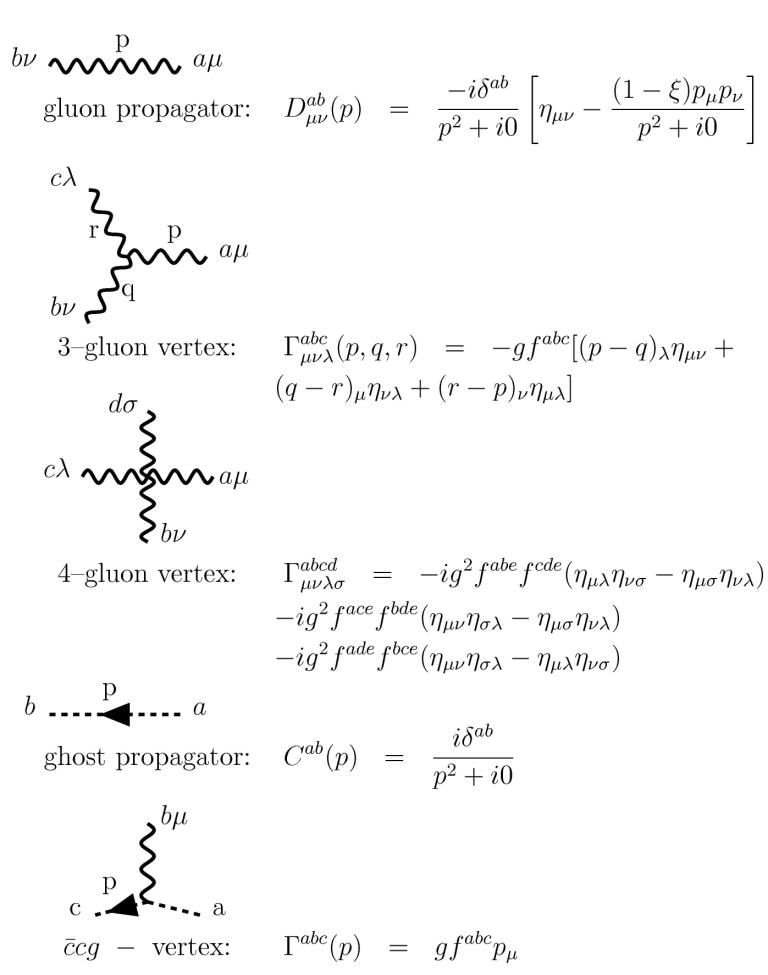
\includegraphics[width=0.8\textwidth]{figures/01-SM-02-QFT/Feynman/yangmills}
% 	\caption{Feynman rules unique to non-abelian Yang-Mills theories, reproduced from Ref.~\cite{enwiki:1243569653}.}
% 	\label{fig:01_qft_gt_yangmills_feynman}
% \end{figure}


% \subsection{Running coupling and asymptotic freedom}
% \label{sec:01_qft_gt_asymptotic}

% As discussed briefly in Section~\ref{sec:01_qft_interactions}, in order to handle divergences from higher order ``loop'' diagrams in perturbation theory, a class of mathematical techniques called \textit{renormalization} is employed.
% A perhaps surprising physical consequence of this is that parameters of the theory are dependent on the energy scale at which they are probed.
% Their dependence is described the \textit{renormalization group equations} or \textit{flow}.

% The renormalization group is an extremely deep subject with applications in many areas of physics.
% The most relevant result for us is the \textit{running} of the coupling constants in gauge theories --- i.e., the strength of the corresponding forces as a function of the energy scale.
% This is shown for the relevant \UU[1], \SU[2], and \SU[3] gauge symmetries of the SM in Figure~\ref{fig:01_qft_running}.

% \begin{figure}[ht]
% 	\centering
% 	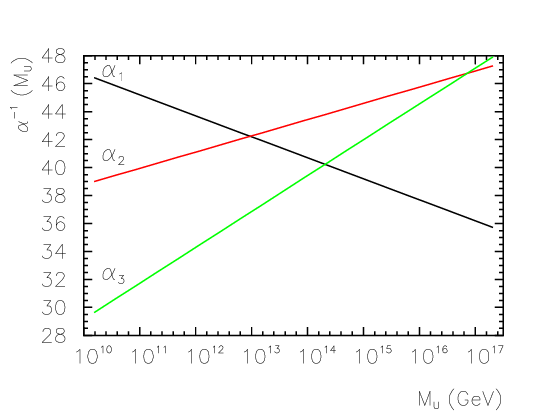
\includegraphics[width=0.8\textwidth]{figures/01-SM-03-SM/qcd/Running-couplings-in-the-standard-model.png}
% 	\caption{The running of the inverse strength of the SM coupling constants, with the strong coupling constant (\SU[3]) in green, weak (\SU[2]) in red, and electromagnetic (\UU[1]) in black, reproduced from Ref.~\cite{Dias2004}.}
% 	\label{fig:01_qft_running}
% \end{figure}

% We see firstly that the electromagnetic interaction strength increases with energy scale.
% Physically, this is understood through the \textit{vacuum polarization} via virtual electron-positron pair creation, which ``screen'' the electric charges of real particles more effectively at longer distances, thereby weakening the force.\footnote{Interestingly, QED has a Landau pole: a finite value of the energy scale for which the interaction strength is infinite. However, this value is so high ($10^{286} \GeV$) as to have no practical consequence, and likely points to the breakdown of perturbation theory, that is used to derive the running coupling, at such a scale.}

% A notable, Nobel-prize winning, 1973 result of Frank Wilczek, David Gross, and David Politzer, however, was an inverse dependence on energy for non-abelian gauge theories~\cite{Politzer:1973fx, Gross:1973id}, as shown for the \SU[2] and \SU[3] couplings in Figure~\ref{fig:01_qft_running}.\footnote{Technically, this depends on the gauge group and the number of fermions in the theory; for both the weak and strong forces, this number is sufficiently small (see e.g. Peskin and Shroeder~\cite{Peskin:1995ev} Chapter 16).}
% This phenomenon is called \textit{asymptotic freedom}, as in the high energy limit the theory is effectively one of free particles.
% It is a notable feature of the strong force, as will be discussed in Chapter~\ref{sec:01_sm_qcd}.


% \section{The ABEGHHK (Higgs) mechanism}
% \label{sec:01_qft_higgs}

% As highlighted in the previous section, gauge bosons in pure Yang-Mills theories are massless.
% This is in conflict, however, with the short observed range of the weak force, implying massive mediatory bosons.
% To resolve this, a series of work in the early 1960s by Anderson, Brout, Englert, Guralnik, Hagen, Higgs, and Kibble (ABEGHHK) yielded a mechanism to give mass to the gauge bosons without violating gauge invariance~\cite{Anderson:1963pc, Englert:1964et, Higgs:1964pj, Guralnik:1964eu}, based on the concept of \textit{spontaneous symmetry breaking} developed by Nambu~\cite{Nambu:1961tp, Nambu:1961fr} and others.

% By 1970, Glashow, Salam, Weinberg and others were able to use this mechanism to formulate a combined theory of weak and electromagnetic interactions, known as ``electroweak'' or Weinberg-Salam theory~\cite{Glashow:1959wxa, Salam:1968rm, Weinberg:1967tq}.
% Electroweak unification has been one of the most significant breakthroughs in theoretical physics with several Nobel prizes cumulatively awarded for these developments.

% In this section we outline the ABEGHHK mechanism --- commonly (but reductively) referred to as the ``Higgs mechanism'' --- first for an abelian gauge theory in Section~\ref{sec:01_qft_higgs_abelian} and then for non-abelian gauge theories~\ref{sec:01_qft_higgs_nonabelian} like the SM.

% \subsection{The abelian Higgs mechanism}
% \label{sec:01_qft_higgs_abelian}

% The Higgs mechanism is based on the idea of spontaneous symmetry breaking (SSB), where the ground states of a physical system violate the overall symmetry.
% The classic example is the so-called ``sombrero'' potential for a complex scalar field $\phi$:
% \begin{equation}
% 	\label{eq:01_qft_higgs_potential}
% 	V(\phi) = -\frac{\lambda}{2}(\abs{\phi}^2 - v^2)^2,
% \end{equation}
% for constants $\lambda$ and $v$, shown in Figure~\ref{fig:01_qft_higgs_potential}.
% The potential has is symmetric under a \UU[1] transformation of $\phi \rightarrow e^{i\alpha}\phi$, but any specific ground state of $\abs{\phi} = v$ will break this symmetry, as shown in the figure.
% SSB is a crucial concept in physics, with several applications in condensed matter and particle physics, including chiral symmetry breaking in QCD (see e.g. Tong SM~\cite{TongSM} Chapter 3.2).

% \begin{figure}[ht!]
% 	\centering
% 	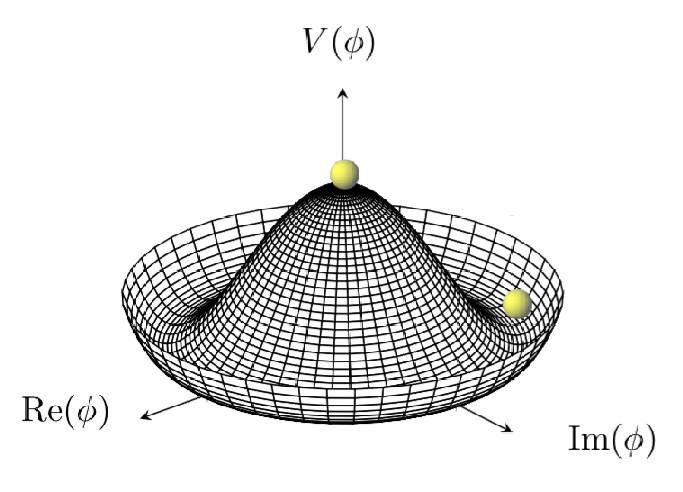
\includegraphics[width=0.7\textwidth]{figures/01-SM-02-QFT/sombrero_potential.png}
% 	\caption{The ``sombrero'' potential for the Higgs field, reproduced from Ref.~\cite{Duff:2020wmn}.
% 	An initial state and a ground state breaking the \UU[1] symmetry are represented by the green balls at the top and bottom of the potential, respectively.}
% 	\label{fig:01_qft_higgs_potential}
% \end{figure}

% The Higgs mechanism is an application of SSB to \textit{gauge} symmetries.
% The interpretation here of SSB a bit fiddly since, as emphasized above, gauge symmetries are not physical and cannot be spontaneously broken;\footnote{This is an implication of Elitzur's theorem~\cite{Elitzur:1975im}.} what actually breaks is the corresponding \textit{global} symmetry, as we outline below.

% Consider our QED Lagrangian for a complex scalar field $\phi$ with the above potential:
% \begin{equation}
% 	\label{eq:01_qft_higgs_lagrangian}
% 	\mathcal L = -\frac{1}{4}F_{\mu\nu}F^{\mu\nu} + (D_\mu\phi)^\dagger D^\mu\phi + \frac{\lambda}{2}(\abs{\phi}^2 - v^2)^2.
% \end{equation}
% As before, this Lagrangian possesses a \UU[1] gauge symmetry; however, this symmetry is ``broken'' by a particular ground state $\phi = v e^{i\delta}$ (we can take $\delta = 0$ WLOG).
% The fluctuations around the ground state can be parametrized as:
% \begin{equation}
% 	\label{eq:01_qft_higgs_fluctuations}
% 	\phi(x) = (v + \sigma(x))e^{i\theta(x)},
% \end{equation}
% where $\sigma$ and $\theta$ are two real fields.
% Plugging this into the Lagrangian gives us:
% \begin{equation}
% 	\label{eq:01_qft_higgs_fluctuations_lagrangian}
% 	\mathcal L = -\frac{1}{4}F_{\mu\nu}F^{\mu\nu} + \partial_\mu\sigma \partial^\mu\sigma + (v + \sigma)^2(\partial_\mu\theta - e A_\mu)(\partial^\mu\theta - e A^\mu) - \lambda(2v^2\sigma^2 + 2 v\sigma^3 + \frac{\sigma^4}{4}).
% \end{equation}
% We see first that $\sigma$ can be interpreted as a normal scalar quantum field, with a quadratic mass term with $m_\sigma^2 = 2\lambda v^2$.
% The $\theta$ term is a bit more unusual;\footnote{In a non-gauge-theory, the $\theta$ field would be considered a massless ``Goldstone boson'' resulting from the spontaneous breakdown of the symmetry.}
% it only appears in the combination $\partial_\mu\theta - e A_\mu$.
% Hence, we can simply redefine the gauge field as $A_\mu' \equiv A_\mu + \frac{1}{e}\partial_\mu\theta$, allowing it to ``absorb'' this DoF.
% Note that this takes the form of a gauge transformation of $A_\mu$ and thus does not affect the field strength tensor $F_{\mu\nu}$.
% The resulting Lagrangian is then:
% \begin{equation}
% 	\label{eq:01_qft_higgs_fluctuations_lagrangian_final}
% 	\mathcal L = -\frac{1}{4}F_{\mu\nu}F^{\mu\nu} + \partial_\mu\sigma \partial^\mu\sigma + e^2(v + \sigma)^2A_\mu'A^{'\mu} - \lambda(2v^2\sigma^2 + 2 v\sigma^3 + \frac{\sigma^4}{4}),
% \end{equation}
% where we now have a mass term for the ``gauge boson'', $m_A^2 = 2e^2 v^2$!

% \subsection{The non-abelian Higgs mechanism}
% \label{sec:01_qft_higgs_nonabelian}

% There is an analogous mechanism for a non-abelian gauge symmetry, as in the SM.
% One crucial difference is that the symmetry may only partially break from the gauge group $G$ to a subgroup $H$ (for example from \SU[2] to a \UU[1]).
% In this case, the gauge bosons corresponding to the generators of $G$'s broken symmetries acquire mass as above, while the generators of $H$ remain massless Goldstone bosons; as we will see in Chapter~\ref{sec:01_sm_ew}, in the SM these correspond to the massive $W^\pm$ / $Z$ bosons and the massless photon, respectively.
% See e.g. Tong SM~\cite{TongSM} Chapter 2.3.3 for an example.


% % \section{Brief encounters with renormalization}
% % \label{sec:01_qft_renormalization}

% %  - perturbation theory leads to infinite integrals at high orders, theory is considered renormalizable if these infinities are canceled or made finite by imposing a cut-off energy scale beyond which the theory is not valid
% %  - implicitly, this means that physical parameters of the theory are not fixed, but depend on the energy scale at which they are measured --- the coupling constants, in particular, are considered to "run" with the energy scale.

% \begin{center}
%   \centering
%   \noindent
%   \textit{If I could remember the names of all these particles, I'd be a botanist.} --- Enrico Fermi
% \end{center}

\chapter{The Standard Model of Particle Physics}
\label{sec:01_sm}

\begin{center}
	\centering
	\noindent
	\textit{Before I came here, I was confused about this subject. Having listened to your lecture, I am still confused. But on a higher level.} --- Enrico Fermi\footnote{Also an accurate representation of my understanding of the SM before and after my PhD.}
\end{center}


\begin{figure}
	\centering
	\captionsetup{justification=centering}
	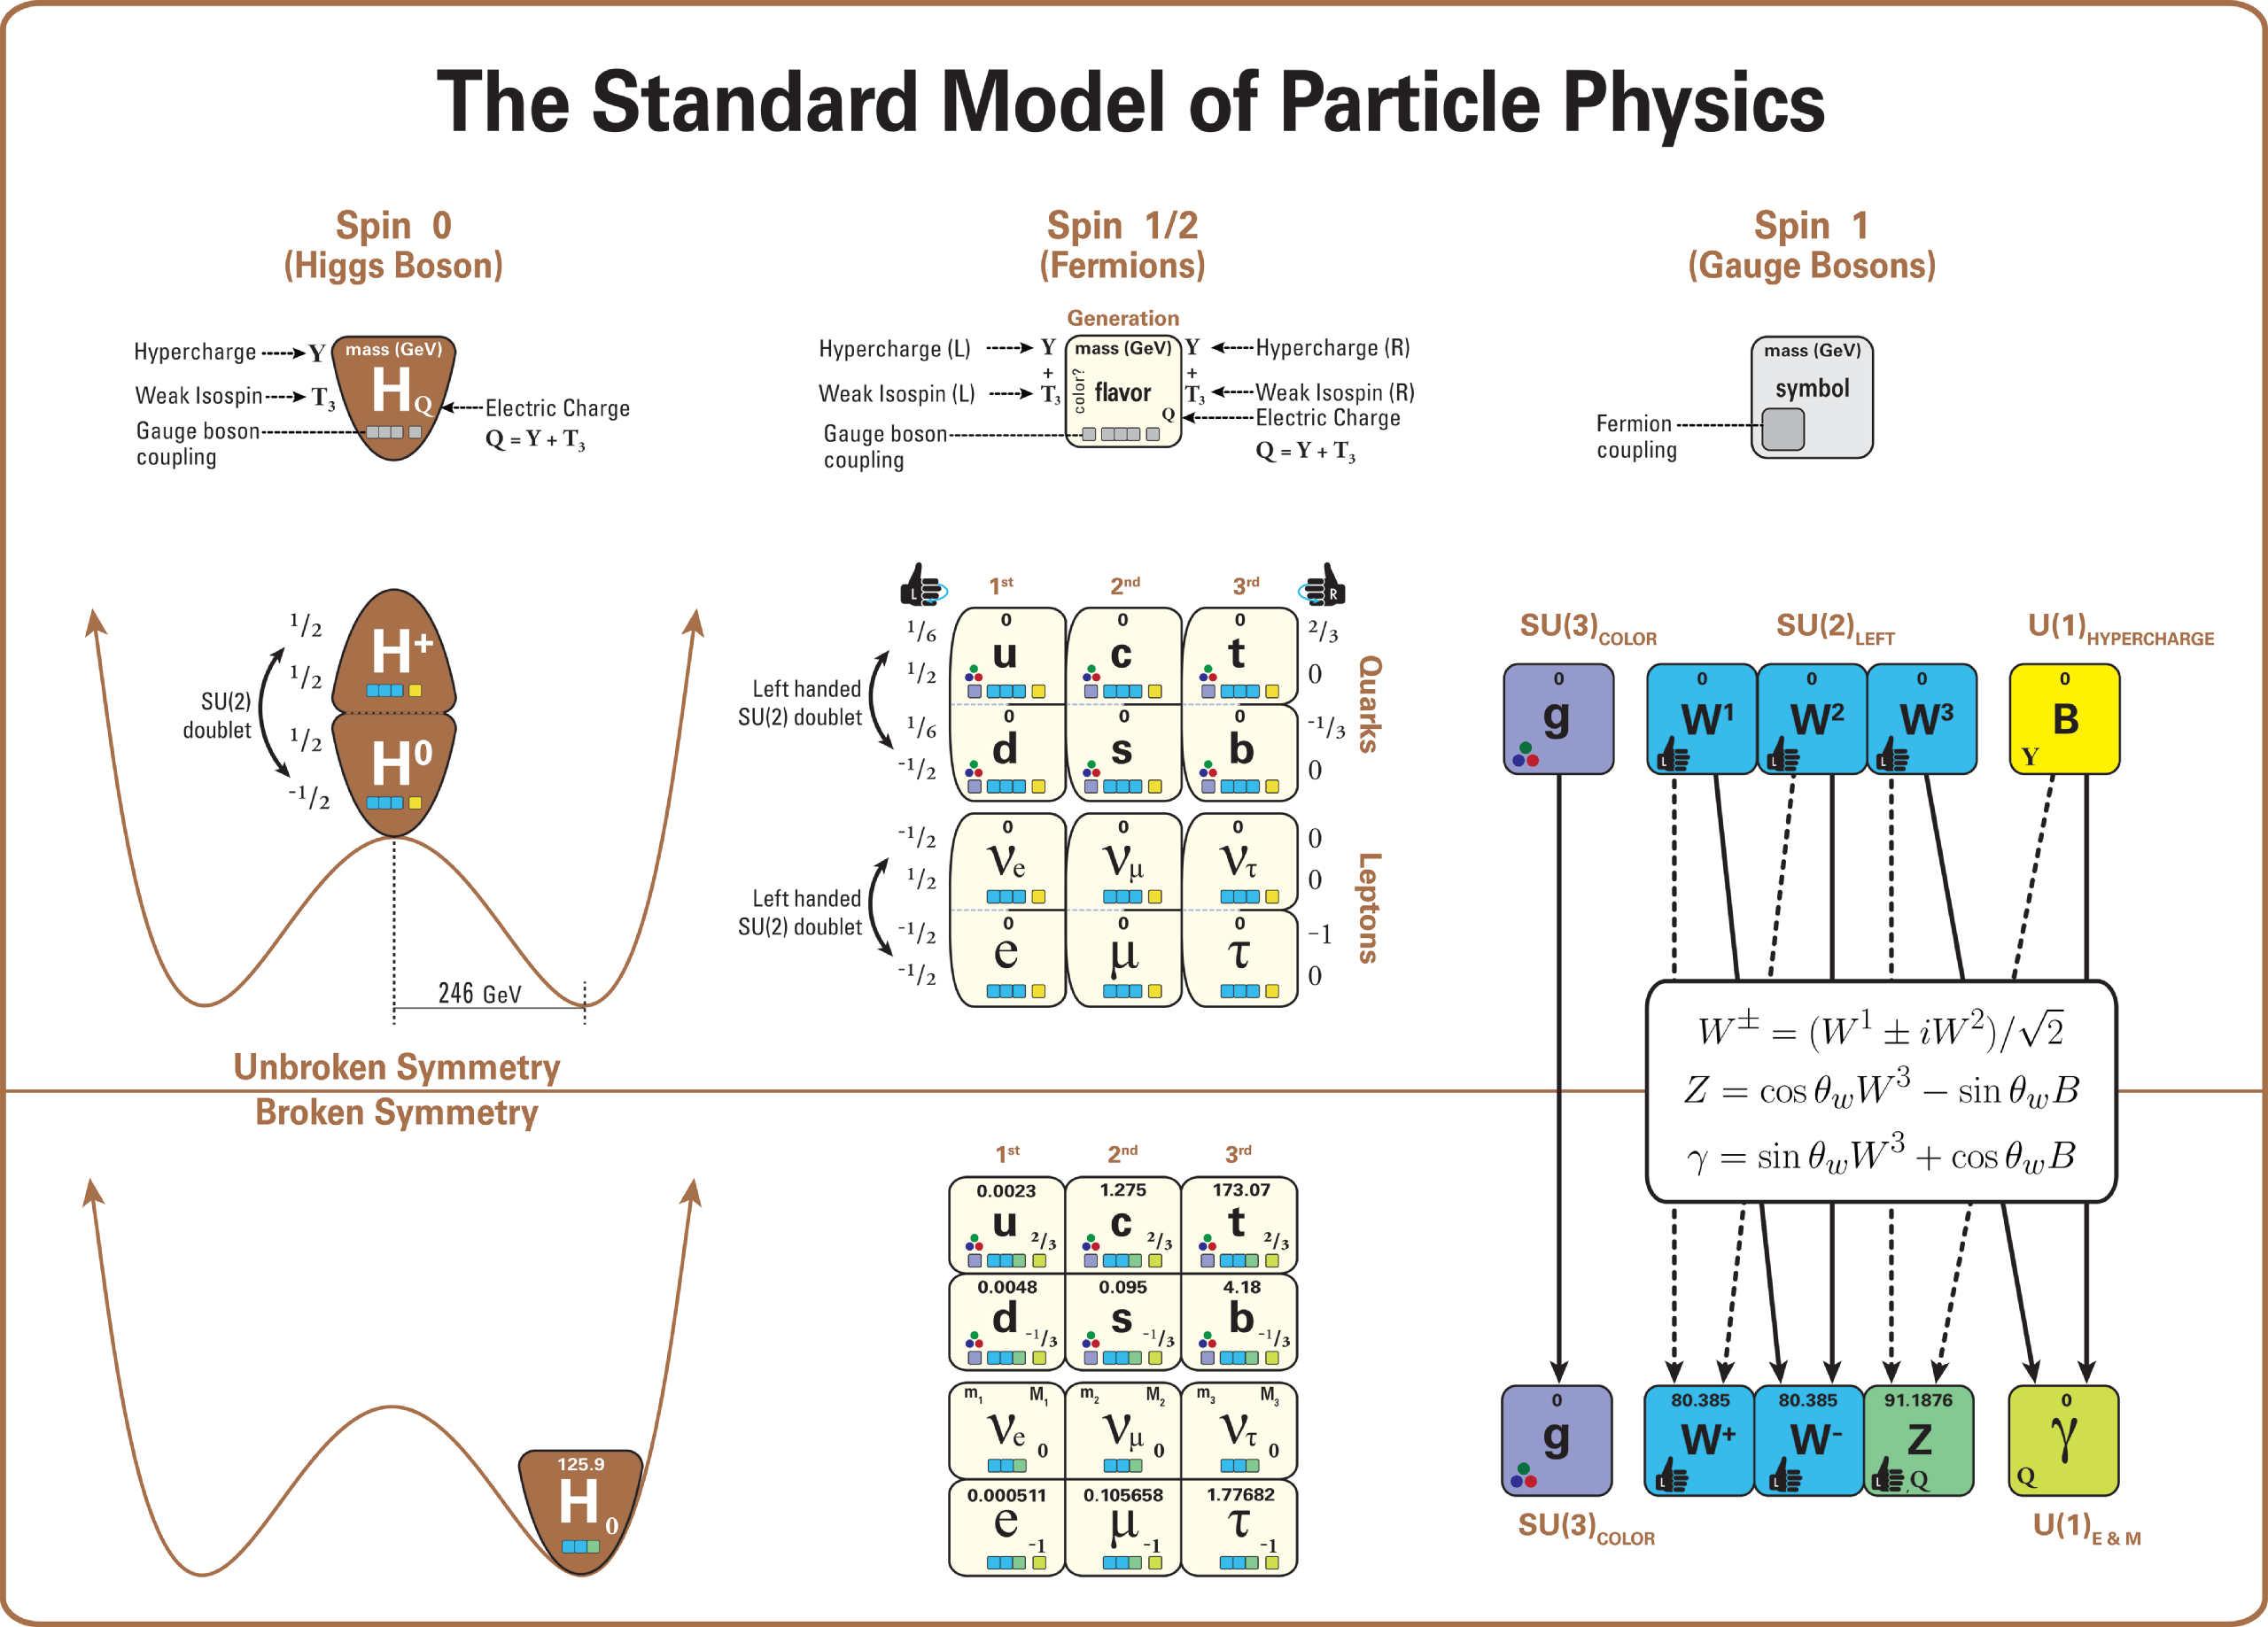
\includegraphics[width=\textwidth]{figures/01-SM-03-SM/Standard_Model_Of_Particle_Physics--Most_Complete_Diagram.png}
	\caption{A graphical summary of the SM, reproduced from Ref.~\cite{SMMostCompleteDiagram}.}
	\label{fig:01_sm_summary}
\end{figure}

We are now ready to describe the standard model (SM)!
It is a renormalizable, quantum Yang-Mills theory, and is illustrated nicely in Figure~\ref{fig:01_sm_summary}.
Before electroweak symmetry breaking (EWSB) --- a form of spontaneous symmetry breaking (SSB) --- it possessed the gauge symmetry $\SU[3]_\mathrm{C} \times \SU[2]_\mathrm{L} \times \UU[1]_\mathrm{Y}$, with $C$, $L$, and $Y$ standing for color, left, and hypercharge, respectively.
%  (their significance will be explained in the following sections).
These three groups correspond to the strong, weak, and electromagnetic forces, with eight, three, and one generators or gauge bosons, respectively.
The relative strengths of each interaction, as well as gravity's, are shown in Table~\ref{tab:01_sm_coupling_constants}, based on the equivalent of the fine structure constant of each force, $\alpha_f = \nicefrac{g_f}{4\pi}$, where $g_f$ is the respective coupling constant.

The SM contains six fermions charged and uncharged under the $\SU[3]_\mathrm{C}$ symmetry each, called the ``quarks'' and ``leptons'', respectively.
% --- the ``quarks'' --- and six fermions uncharged --- the ``leptons''.
The left-handed fermions live as pairs in $\SU[2]_\mathrm{L}$ doublets, while the right-handed fermions in singlets.
The six types of fermions are referred to as different ``flavors'', grouped into three generations as in Figure~\ref{fig:01_sm_summary}.

The SM also contains a complex scalar $\SU[2]_\mathrm{Y}$-doublet called the Higgs field, which is associated with EWSB.
As shown in Figure~\ref{fig:01_sm_summary}, it initially is at the center of a ``sombrero'' potential because of which, before EWSB, the gauge bosons, fermions, and the Higgs field are all massless.

% where the subscripts will be explained in the following sections, with massless gauge bosons and fermions a zero vacuum expectation value (VEV) for the Higgs field.
EWSB is hypothesized to have occurred during the electroweak epoch (see Figure~\ref{fig:00_timeline}), where the $\SU[2]_\mathrm{L} \times \UU[1]_\mathrm{Y}$ global symmetry broke to the $\UU[1]_\mathrm{EM}$ of QED.
Through this, the Higgs field obtained a non-zero vacuum expectation value (VEV), imbuing all the fermions, three of the gauge bosons, and the Higgs boson with mass --- a process referred to as the Higgs mechanism.
The outcome is the state of the universe and physics as we know it.

Of course, as outlined in the introduction, this picture does not explain myriad phenomena in fundamental physics, including dark matter, dark energy, baryon asymmetry, and neutrino masses.
This is why it is crucial to test the SM as rigorously and in as broad a phase space as possible, in order to identify any cracks that may point to new physics.

% The relative strength of each of their interactions is typically quantified by the equivalent of the fine structure constant for each force, $\alpha_f = \nicefrac{g_f}{4\pi}$, where $g_f$ is the coupling constant.
% This is shown in Table~\ref{tab:01_sm_coupling_constants} for each force, as well as gravity for illustrative purposes.

\begin{table}[htbp]
    \centering
	\renewcommand{\arraystretch}{1.5}
    \begin{tabular}{ll}
        \toprule
        \textbf{Force} & \textbf{Strength}\\
        \midrule
        Electromagnetic &
        $\alpha_\mathrm{EM} \approx \frac{1}{137}$ \\
        Weak &
        $\alpha_W \approx \frac{1}{30}$\\
        Strong &
        $\alpha_s \approx 1$\\
        Gravity &
        $\alpha_G  \approx 10^{-38}$\\
        \bottomrule
    \end{tabular}
	\vspace{5mm}
	\caption{Approximate magnitude of the strengths of the four fundamental forces at an energy scale of around 100\MeV.}
	\label{tab:01_sm_coupling_constants}
\end{table}

In this chapter, we will briefly walk through different areas of the SM.
Having discussed QED in Chapter~\ref{sec:01_qft_gt}, we begin with the remaining two fundamental interactions: quantum chromodynamics (Section~\ref{sec:01_sm_qcd}); and weak interactions and electroweak unification (Section~\ref{sec:01_sm_ew}).
% As we will see, the phenomenology of these forces is dictated by the ``running'' of their coupling constants; i.e., the dependence of the strength of the interactions on the energy scale at which they are probed, plotted in Figure~\ref{fig:01_sm_running}.
Finally, in Section~\ref{sec:01_higgs}, we will discuss the Higgs sector and pair production of the Higgs boson, which is the focus of this dissertation.


\section{Quantum chromodynamics}
\label{sec:01_sm_qcd}

Quantum chromodynamics (QCD) is a quantum Yang-Mills field theory describing the strong force, with the gauge group $\SU[3]$.
$\SU[3]$ has eight generators and, hence, eight gauge bosons ($G_\mu$) called gluons.
The only other elementary particles which interact with the strong force --- i.e., which don't live in the trivial representation of $\SU[3]$ --- are the quarks.
They live in the three-dimensional fundamental representation and thus possess three extra DoFs beyond vanilla spinors, which we call their ``color'' (hence, quantum \textit{chromo}dynamics).
The three orthogonal eigenstates in this representation are colloquially referred to as labeled red, green, and blue, and mathematically the quark fields ($q_\alpha$) labeled with extra color indices $i = 1, 2, 3$.

Putting this together, the QCD Lagrangian, with all the indices labeled explicitly is:
\begin{equation}
	\label{eq:01_sm_qcd_lagrangian}
	\mathcal L = -\frac{1}{4} G^a_{\mu\nu} G^{a\mu\nu} + \sum_{f = 1}^6 \bar q_{\alpha f i} [\delta_{ij}(i\slashed \partial_{\alpha\beta} - m \delta_{\alpha\beta}) + g_s \slashed G^a_{\alpha\beta} t_{ij}^a] q_{\beta f j}
\end{equation}
where $g_s$ is the strong coupling constant, $G^a_{\mu\nu} = \partial_\mu G^a_\nu - \partial_\nu G^a_\mu + g_s f^{abc} G^b_\mu G^c_\nu$ is the gluon field strength tensor, $f^{abc}$ are the structure constants of $\SU[3]$, $t^a$ are the generators of $\SU[3]$ in the fundamental representation, the sum over $f$ is running over the six flavors, and the indices $a$ and $i, j$ label the eight gluons and the three colors of quarks, respectively.
The six flavors of quarks have different masses and charges, as shown in Figure~\ref{fig:01_sm_qcd_quarks}.

\begin{figure}[ht]
	\centering
	\captionsetup{justification=centering}
	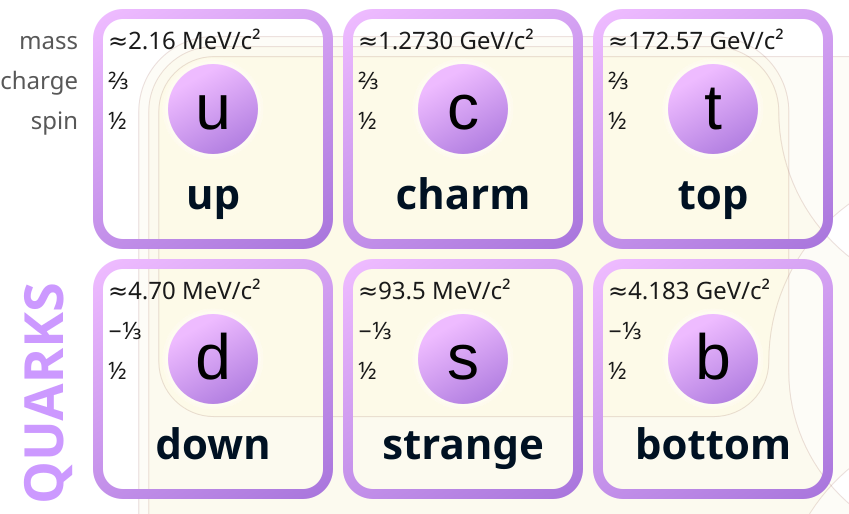
\includegraphics[width=0.5\textwidth]{figures/01-SM-03-SM/qcd/quarks.png}
	\caption{The quarks in the SM, reproduced from Ref.~\cite{enwiki:1238968997}.}
	\label{fig:01_sm_qcd_quarks}
\end{figure}

QCD is an extremely rich and complex theory due to its non-abelian gauge symmetry, the six different flavors of quarks, and the unique strength and running of its coupling, shown in Figure~\ref{fig:01_sm_qcd_running}.
Observe its property of weak coupling and asymptotic freedom at high energies, versus the extremely high $\mathcal O(1)$ value of $\alpha_s$ at low energies leading to the phenomenon of \textit{confinement}.
Note also that $\alpha_s$ appears to diverge in Figure~\ref{fig:01_sm_qcd_running} at around $200 \MeV$, a sign of perturbation theory breaking down. 
This $200 \MeV$ limit is considered the characteristic energy scale of QCD, $\Lambda_\mathrm{QCD}$.\footnote{The phenomenon of an energy scale arising from a dimensionless coupling constant  is known as \textit{dimensional transmutation} (see e.g. Tong SM~\cite{TongSM} Chapter 3).}

\begin{figure}[ht]
	\centering
	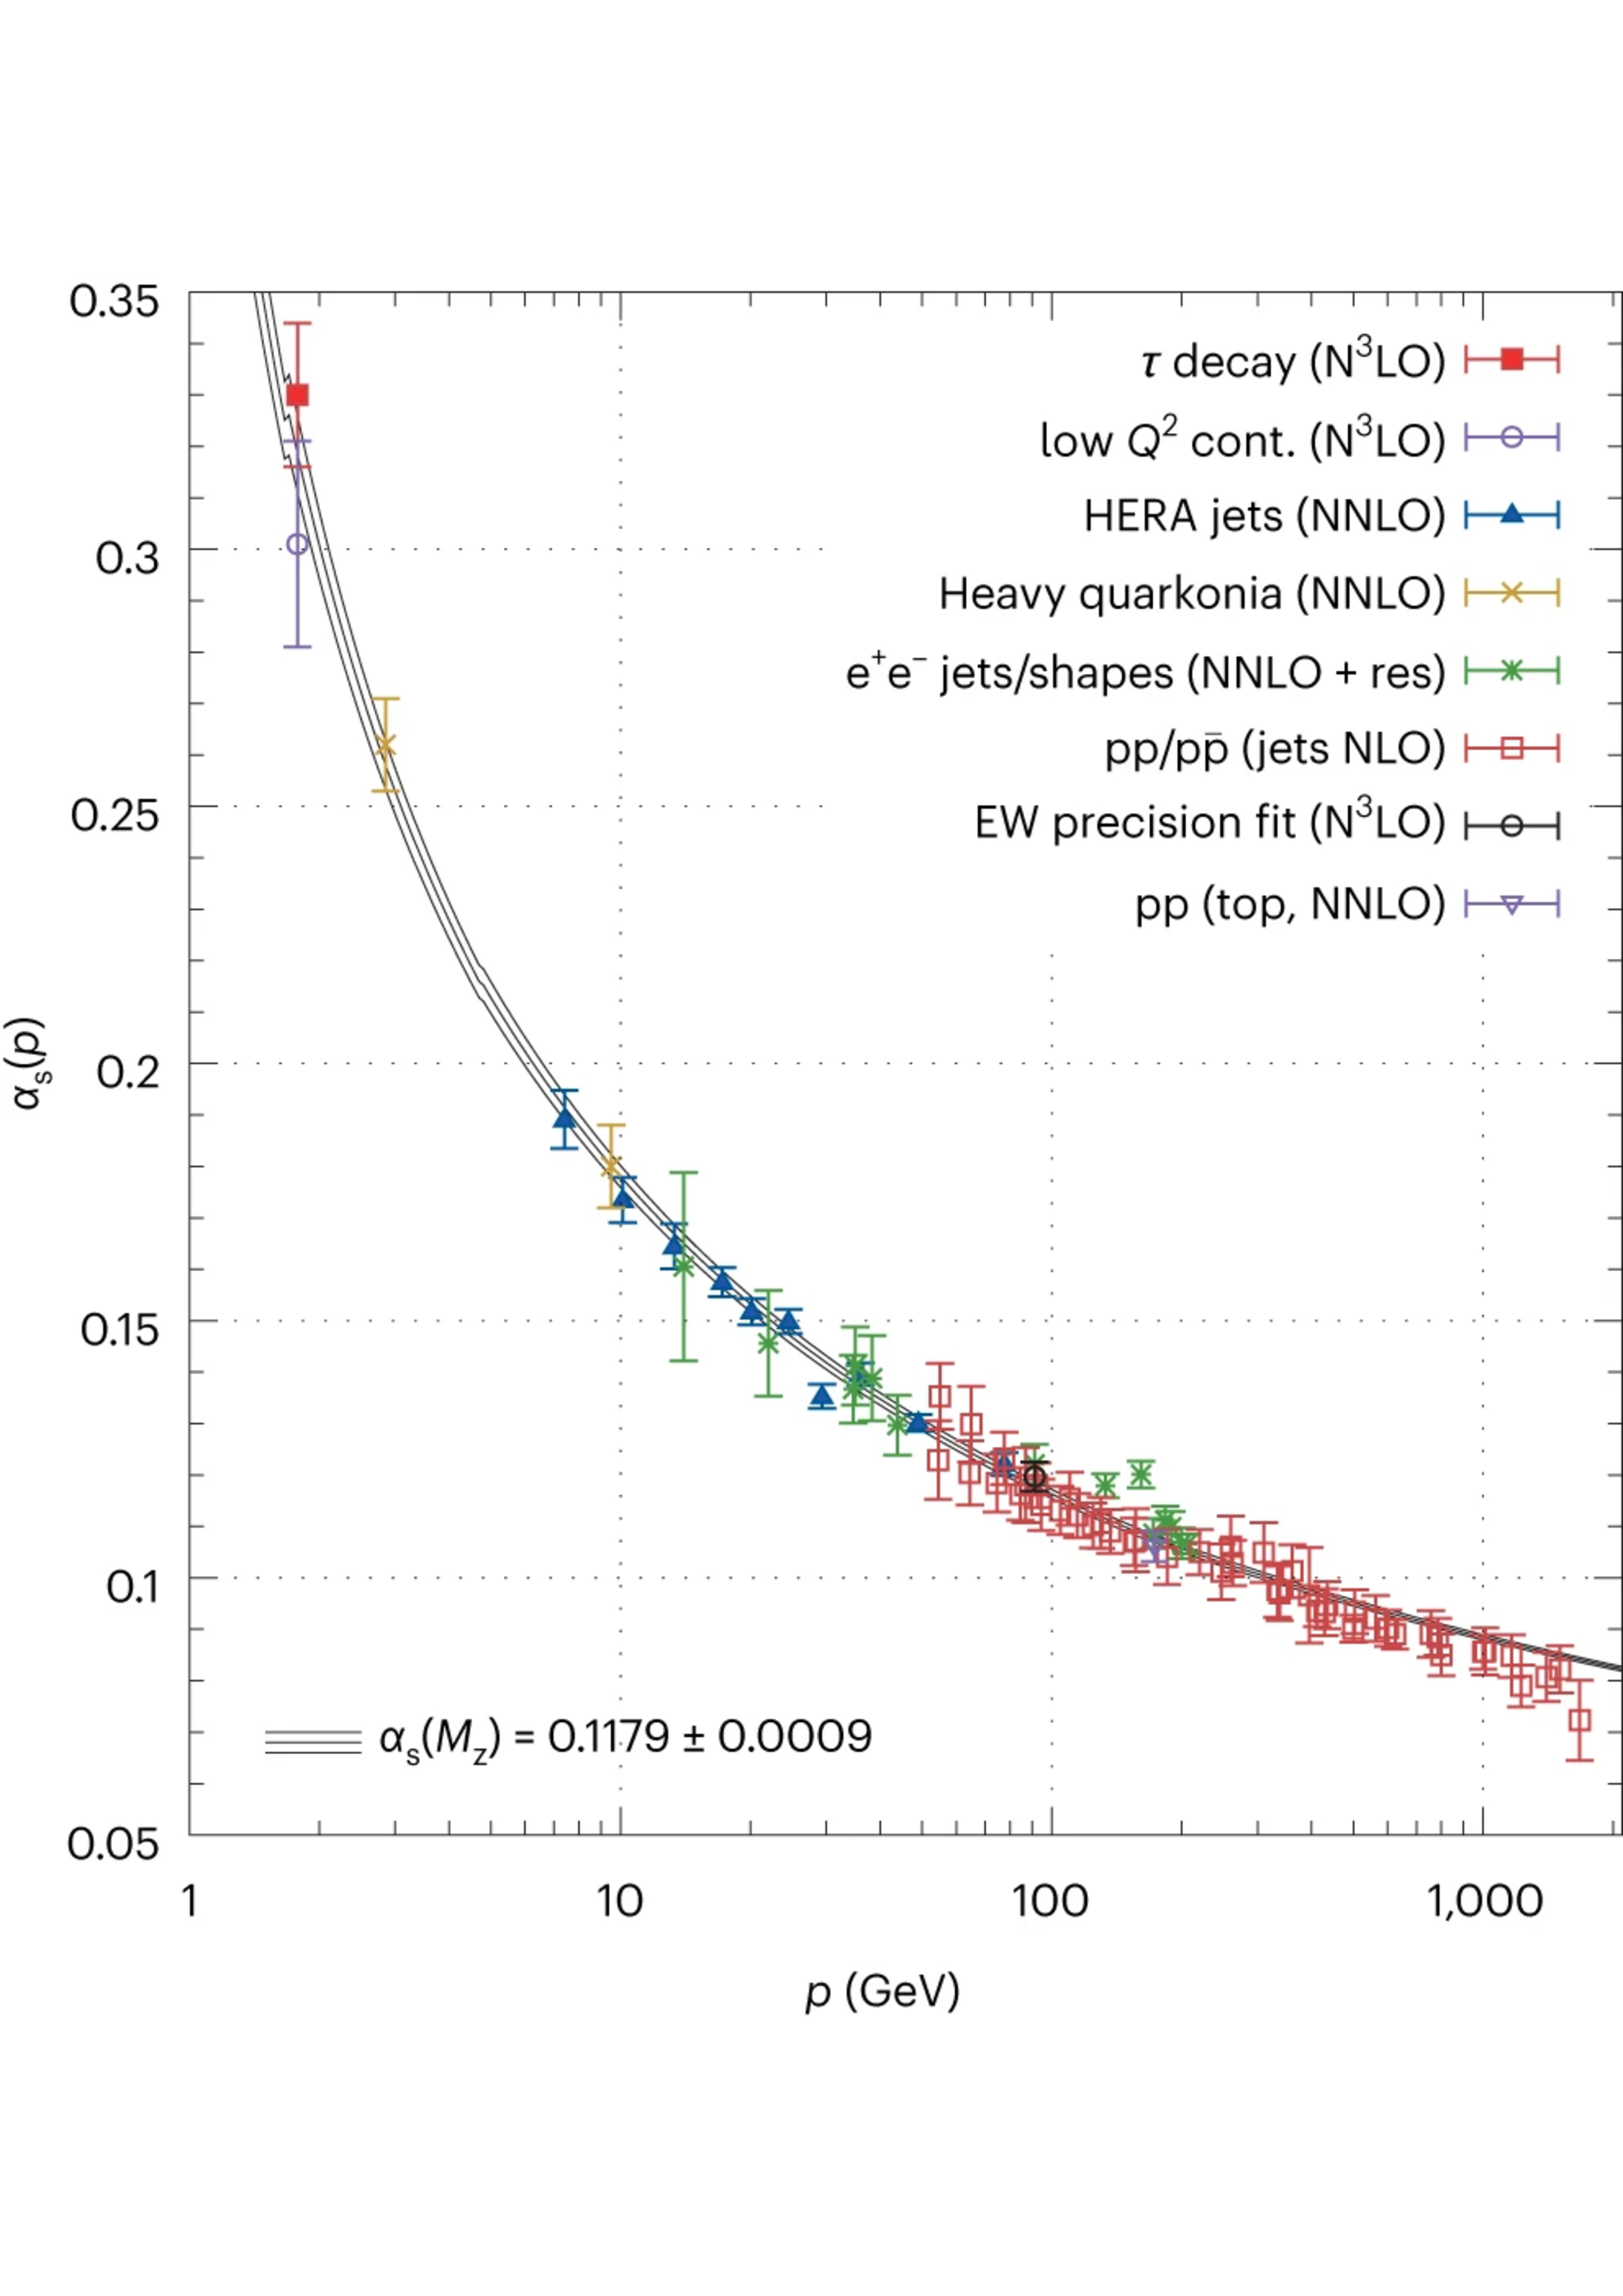
\includegraphics[width=0.5\textwidth]{figures/01-SM-03-SM/qcd/qcd_running}
	\caption{The theoretically predicted running of the strong coupling $\alpha_s = \nicefrac{g_s^2}{4\pi}$ as a function of the energy scale along with experimental measurements, reproduced from Ref.~\cite{Boito:2023lzf}.}
	\label{fig:01_sm_qcd_running}
\end{figure}

The $\mathcal O(1)$ coupling strength means that the standard perturbative techniques we have discussed are not applicable at our usual energy scales; instead, we must rely on nonperturbative techniques such as numerical simulations of QCD on a discretized spacetime lattice (see e.g. Schwartz~\cite{Schwartz:2014sze} Chapter 25).
Because of this, QCD is one of the least understood and most exciting areas of study in modern physics.

% \TODO{Organization of this section}


\subsection{Asymptotic freedom and confinement}
\label{sec:01_sm_qcd_asymptotic}

As discussed above, a key phenomenological characteristic of the strong force is asymptotic freedom, wherein at high energies quarks and gluons behave as free particles.
This also means that perturbative techniques can be applied at high energies; indeed, we can derive an analogous $\nicefrac{1}{r^2}$ ``Coulomb force'', based on tree-level quark-quark scattering amplitudes, for quarks at very short distances.
This force turns out to always be attractive between quarks and antiquarks, as well as between two or even three quarks in different color states: the ``aim'' of the force appears to always be to form color-neutral bound states.
These are called \textit{mesons} for the case of an antiquark and quark pair, and \textit{baryons} for three quarks.

At longer distances we enter the strong-coupling and nonperturbative regime, in which the dynamics are harder to understand.
However, through lattice QCD simulations, we are able to see the emergence of a ``flux tube'' pulling quarks together as they are pushed apart, as shown in Figure~\ref{fig:01_sm_qcd_fluxtubes}.
This phenomenon is referred to as \textit{confinement}, and it means we can never observe free quarks or gluons outside high-energy colliders.
Both the long- and short-distance behavior of the strong force conspire to always confine quarks in color-neutral hadrons.
The scale of confinement is naturally set by $\Lambda_\mathrm{QCD} \approx 200 \MeV$, which is hence roughly the radius of the proton and other hadrons ($1$fm in SI).

\begin{figure}[ht]
	\centering
	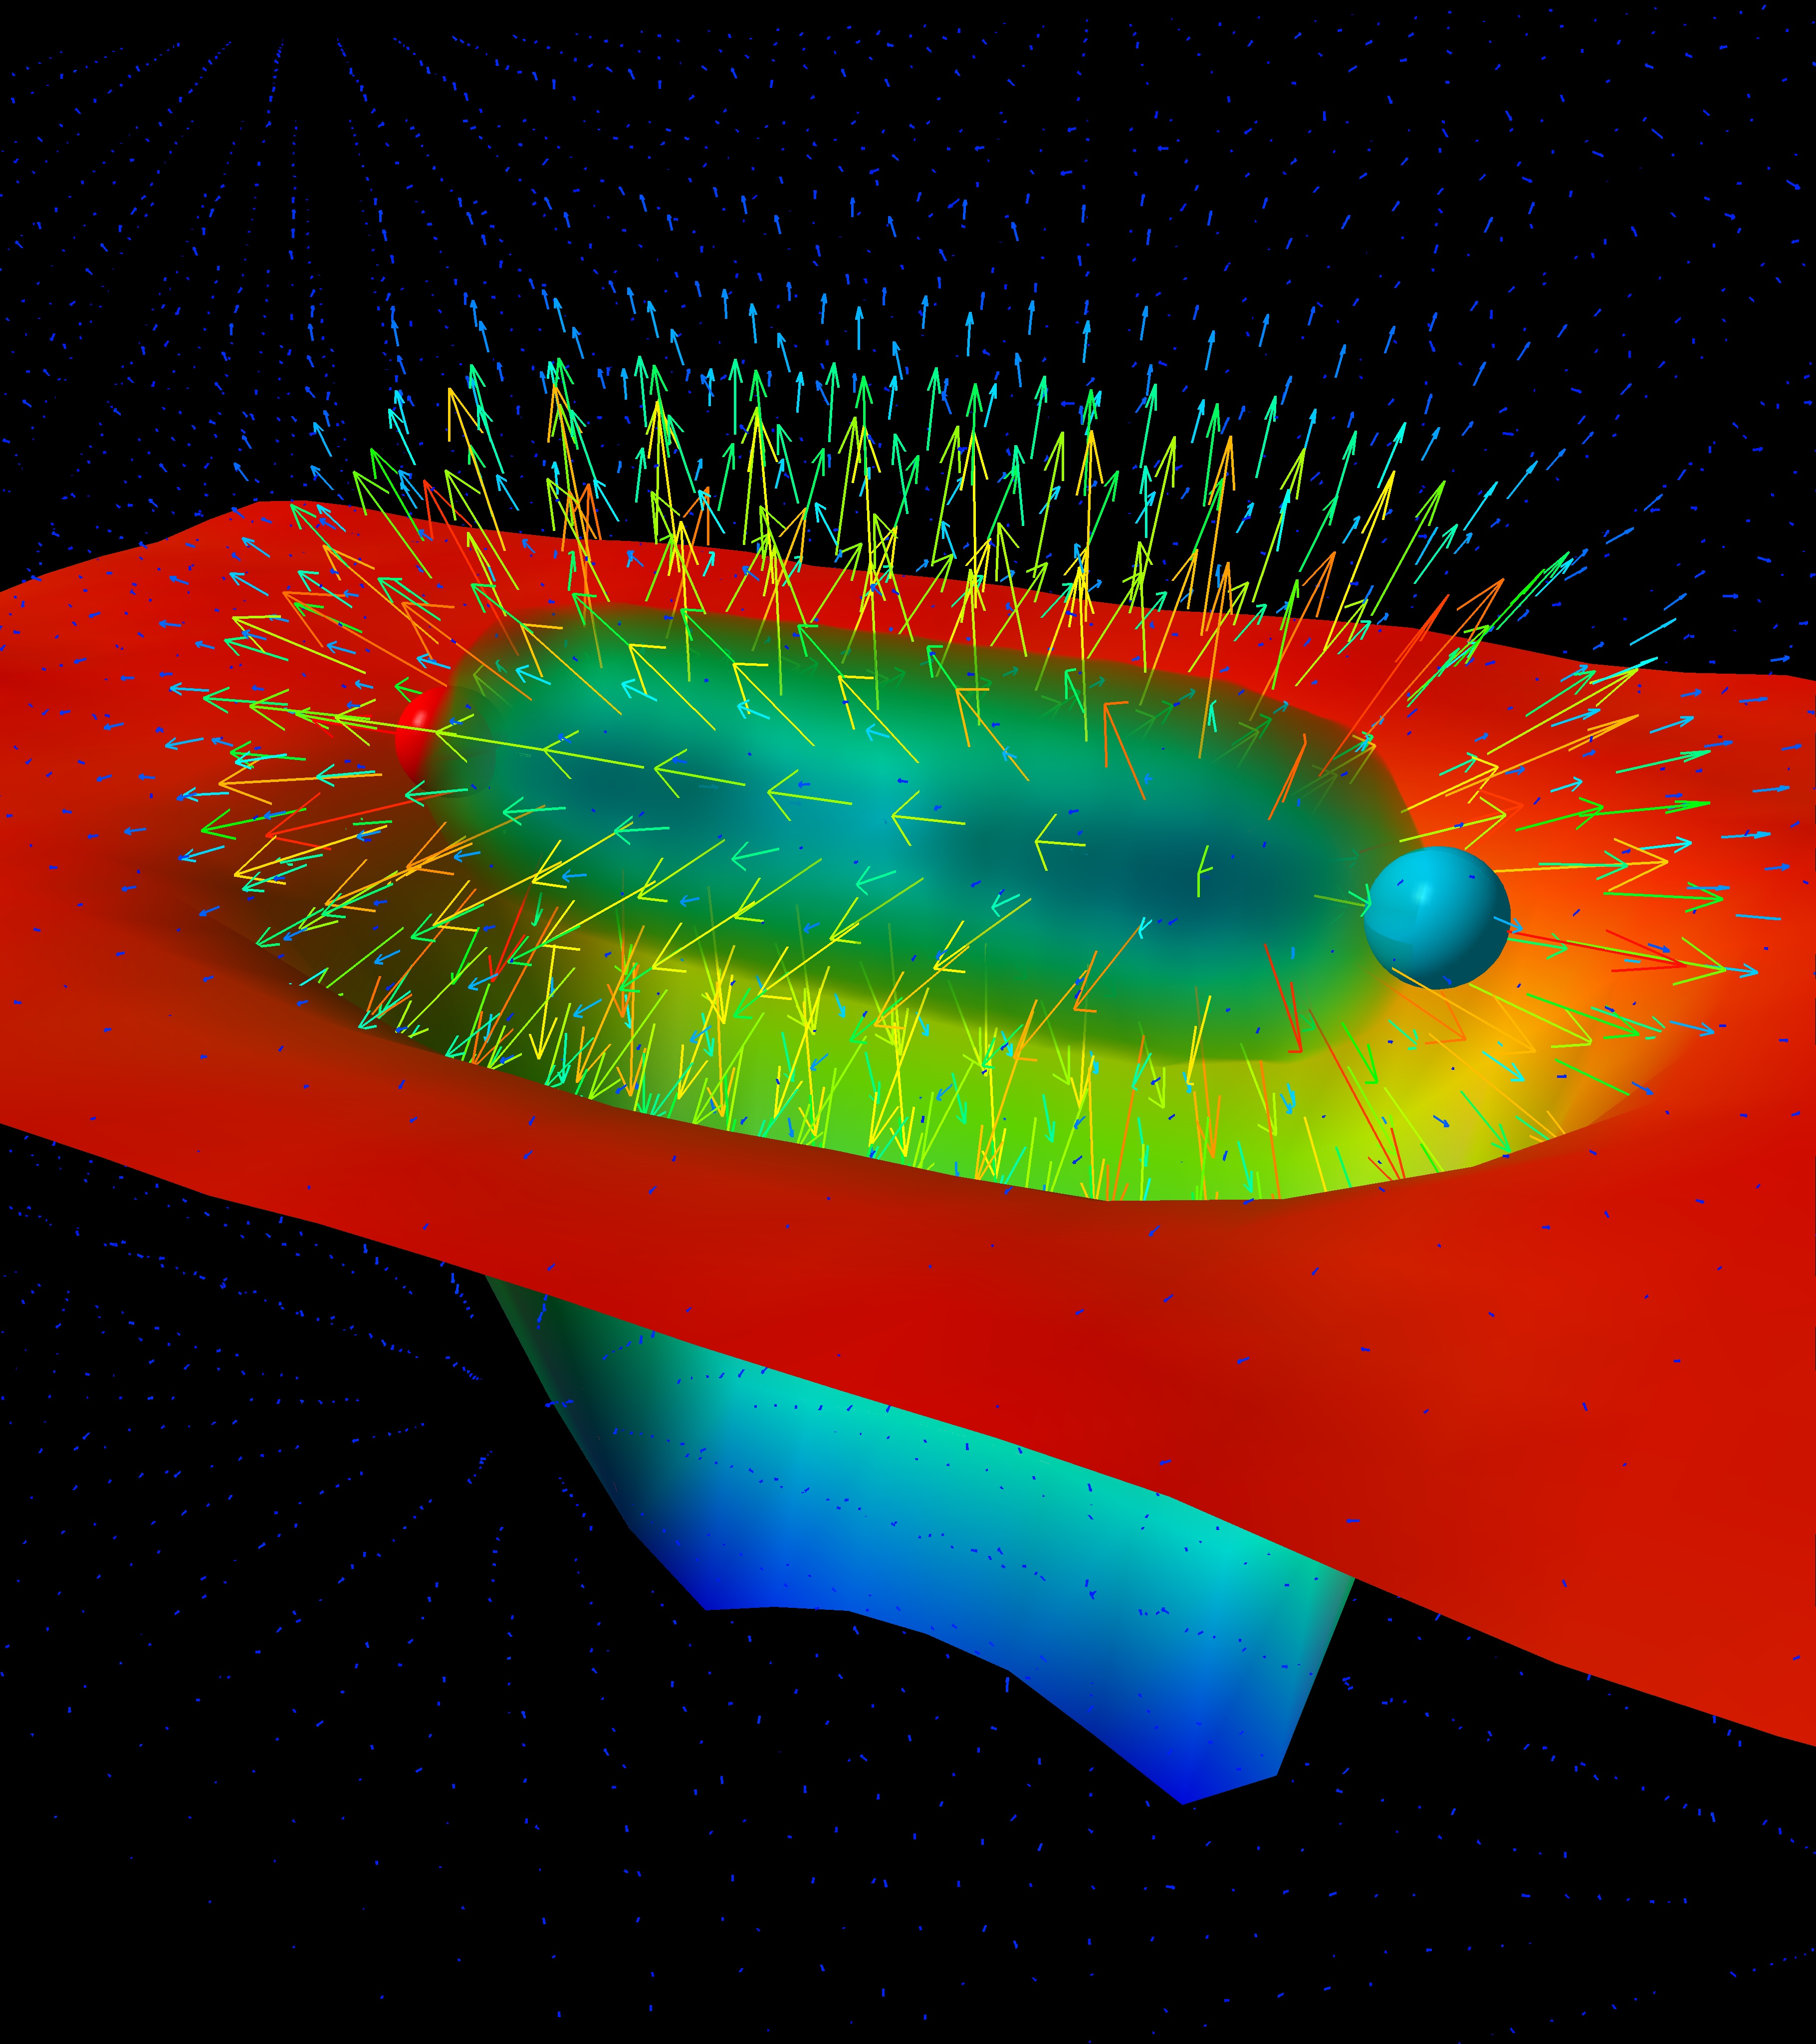
\includegraphics[height=7cm]{figures/01-SM-03-SM/qcd/FluxTube.jpg}
	\hspace{2mm}
	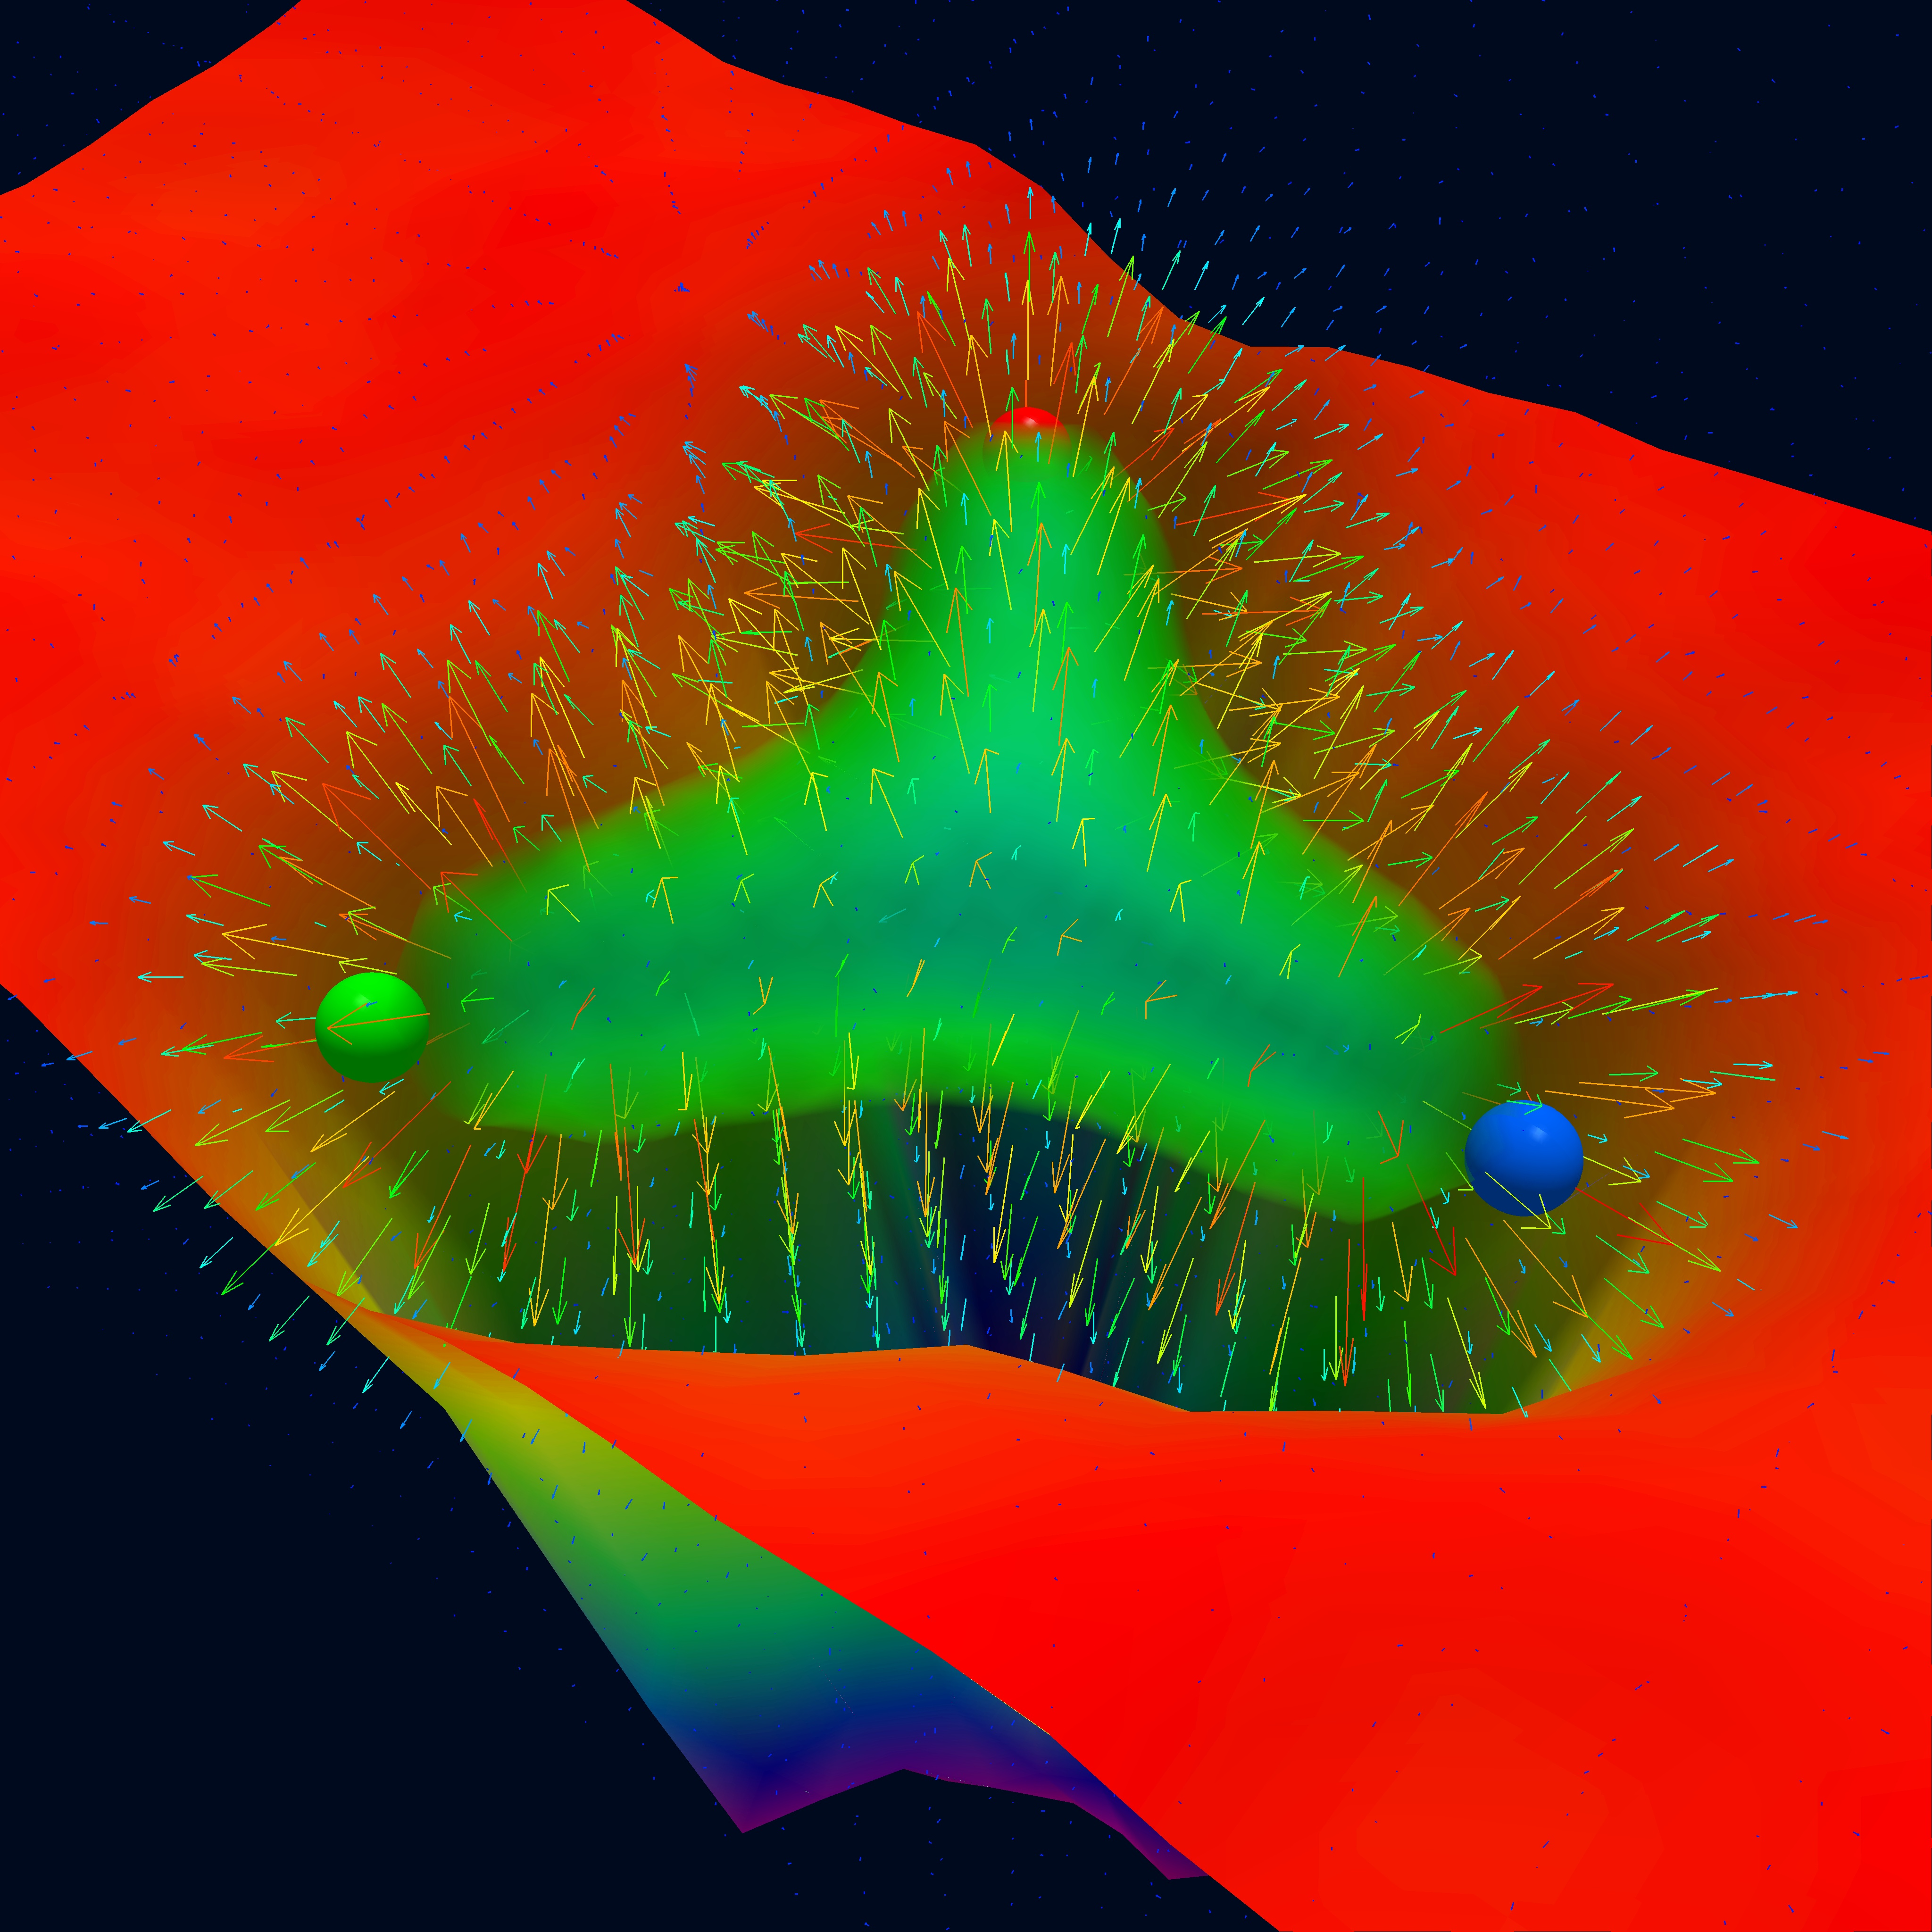
\includegraphics[height=7cm]{figures/01-SM-03-SM/qcd/VacuumRespAction16t32_YshapeCSSMcover.jpg}
	\caption{``Flux tubes'' between a quark and anti-pair inside a meson (left) and three quarks in a proton (right), reproduced from Refs.~\cite{Bissey:2006bz, LeinweberVisualQCD}.}
	\label{fig:01_sm_qcd_fluxtubes}
\end{figure}


\subsection{Quarks and the eightfold way}
\label{sec:01_sm_quarks}

Since their discovery in the 1920s and 30s, the proton and neutron and were believed to be elementary particles along with the electron and photon.
In fact, due to confinement, the first experimental evidence of quarks was not found until the 1960s.
However, already in 1932, the remarkably similar masses of the two nucleons surprised physicists and led Heisenberg, Wigner, and others to hypothesize an underlying \SU[2] symmetry between them (later named \textit{isospin})~\cite{Heisenberg1932, Wigner1937}.
The intrigue only increased in the next decades, during which new cosmic ray, cyclotron, and bubble chamber experiments discovered a veritable ``zoo'' of hadrons, exemplified by a 1964 table of particles in Figure~\ref{fig:01_sm_qcd_particle_zoo}.
While all appeared elementary, several had surprisingly similar properties such as mass and spin, and could also be grouped into invariant subspaces of the isospin group.

\begin{figure}[ht]
	\centering
	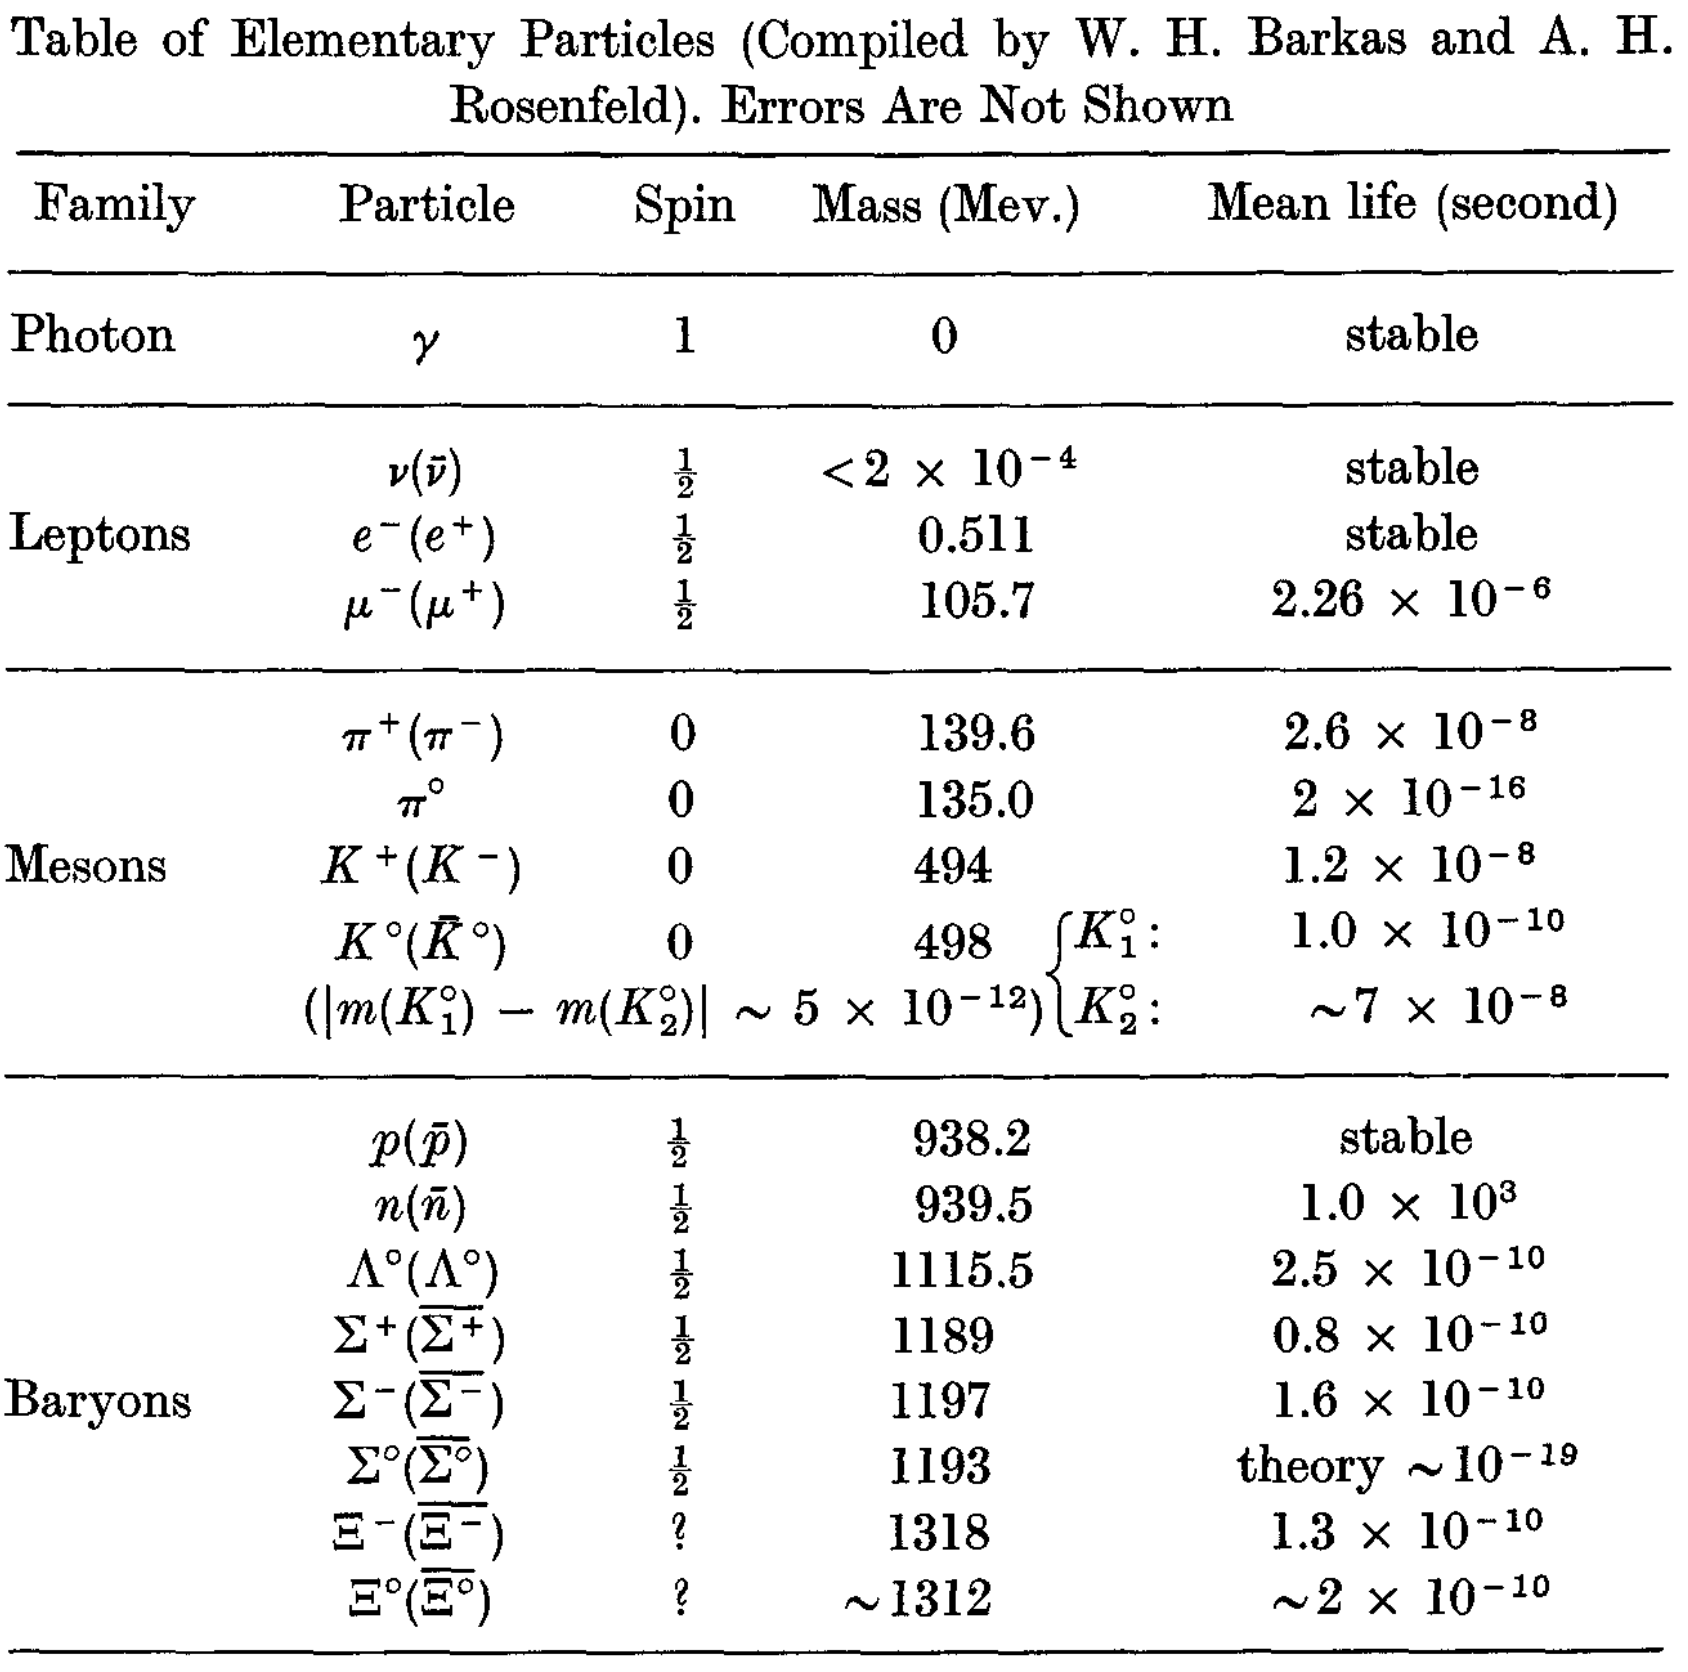
\includegraphics[width=0.8\textwidth]{figures/01-SM-03-SM/qcd/table_elementary_particles_sakurai.png}
	\caption{A table of what were considered to be elementary particles in 1964, reproduced from Ref.~\cite{Sakurai:2015gmk}.}
	\label{fig:01_sm_qcd_particle_zoo}
\end{figure}

In 1961, Murray Gell-Mann and Yuval Ne'eman independently realized that the new hadrons could elegantly fit into representations of a larger symmetry group, \SU[3]~\cite{Gell-Mann:1961omu, Neeman:1961jhl}.
Gell-Mann and George Zweig in 1964 then independently showed that this could be explained physically by hadrons being composed of combinations of three fundamental particles, named the ``up'', ``down'', and ``strange quarks'', with the former two carrying isospin up and down, respectively~\cite{Gell-Mann:1964ewy, Zweig:1964jf}.
% \footnote{Although, interestingly, Gell-Mann himself thought of them as mathematical conveniences than real particles.}
Gell-Mann named this model the ``eightfold way'' (since $\dim (\SU[3]) = 8$) and was awarded the Nobel Prize in 1969 for this work.

Examples of baryons (three-quark hadrons) in the octet and decuplet (dimension 8 and 10, respectively) representations of $\SU[3]$ are shown in Figure~\ref{fig:01_sm_qcd_eightfoldway}, sorted by their isospin along the ``z'' axis ($I_3 = $ \# of up quarks - \# of down quarks) and strangeness ($S = $ \# of strange quarks).
Note that this \SU[3] symmetry is only approximate; it is broken by the different masses of the quarks.
However, their significantly smaller masses compared to $\Lambda_\mathrm{QCD}$ mean it remains a useful symmetry for categorizing hadrons.
On the other hand, broader ``symmetries'' such as \SU[4] through \SU[6] including the heavier charm, bottom and top quarks are broken so heavily by their higher masses that they are not helpful for characterizing the heavier hadrons.

\begin{figure}[ht]
	\centering
	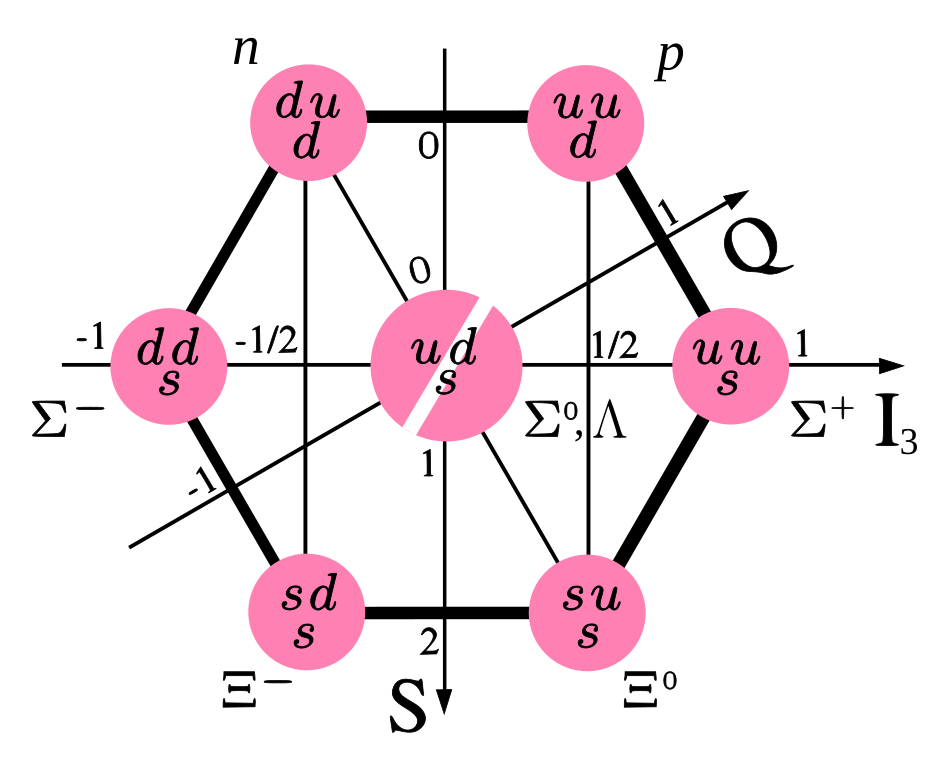
\includegraphics[width=0.45\textwidth]{figures/01-SM-03-SM/qcd/Baryon-octet-small.svg.png}
	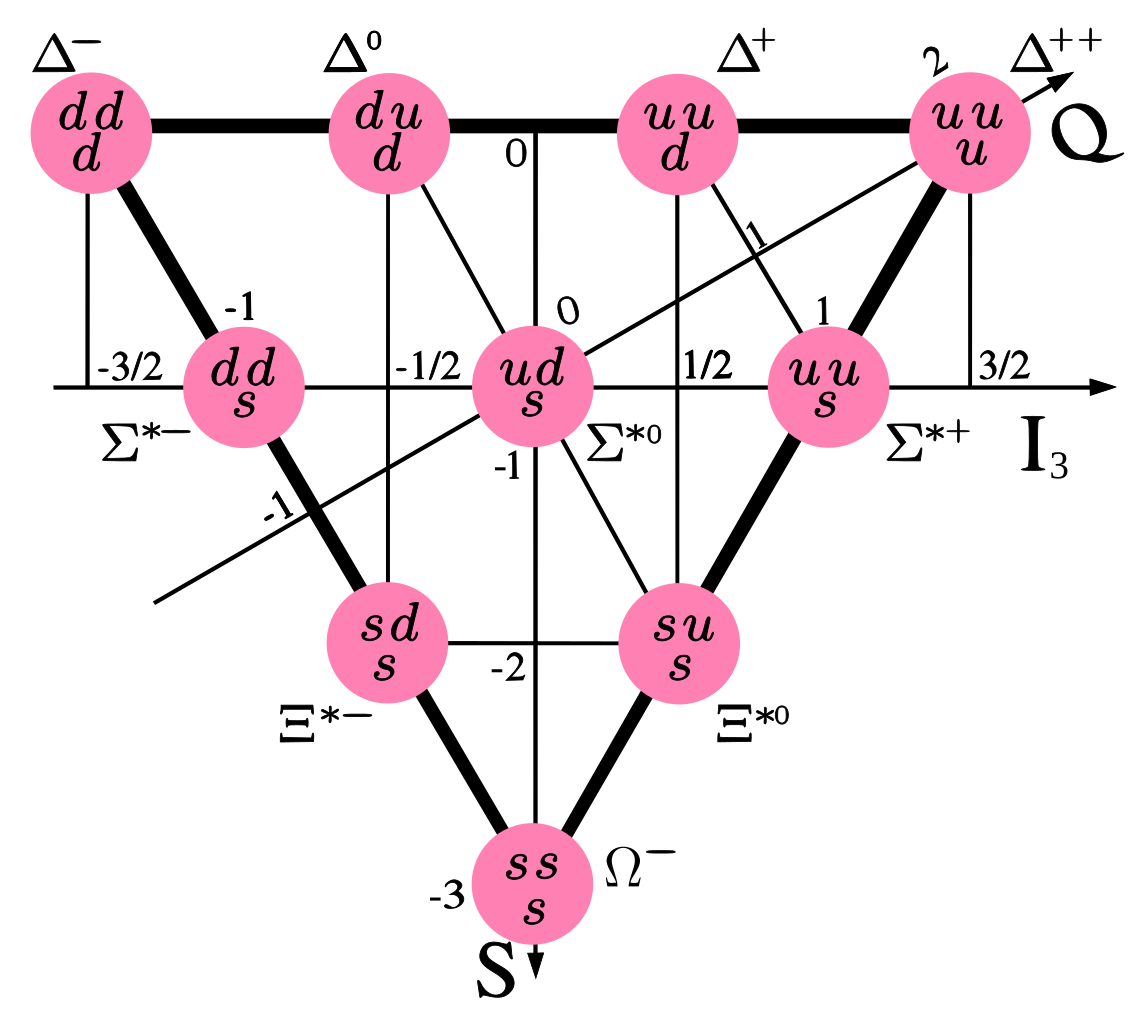
\includegraphics[width=0.45\textwidth]{figures/01-SM-03-SM/qcd/Baryon-decuplet-small.svg.png}
	\caption{Baryons in the octet (left) and decuplet (right) representations of $\SU[3]$, reproduced from Ref.~\cite{enwiki:1243626239}.}
	\label{fig:01_sm_qcd_eightfoldway}
\end{figure}

This fourth ``charm'' quark was notably predicted by Sheldon Glashow, John Iliopoulos, and Luciano Maiani in 1970 to explain the observed suppression of $Z$-boson-mediated flavor-changing neutral currents~\cite{Glashow:1970gm} (and also to match the number of known leptons at the time).
This, and the quark model as a whole, was famously validated by the discovery of a $3.1 \GeV$ charm-anti-charm bound state, named the $J/\psi$ meson, simultaneously by Burton Richter's team at the Stanford Linear Accelerator Center (SLAC) and Samuel Ting's team at Brookhaven National Laboratory in 1974~\cite{SLAC-SP-017:1974ind, E598:1974sol}, both of whom received the Nobel Prize in 1976.

A year before this, Makoto Kobayashi and Toshihide Maskawa had proposed the existence of a \textit{third} generation of quarks to explain the observed CP-violation in weak interactions~\cite{Kobayashi:1973fv}.
This proposal gained more traction after the $J/\psi$ discovery, as well as the discovery of a third-generation lepton, the $\tau$, by Martin Lewis Perl's team in electron-positron collisions at SLAC between 1973 and 1977~\cite{Perl:1975bf}.

In the end, both third generation quarks were discovered at the Fermi National Accelerator Laboratory (Fermilab): first the bottom quark in 1977 by Leon Lederman's team on the E288 experiment~\cite{E288:1977xhf}; and then, much later, the top quark in 1995 by the CDF and DØ experiments at the Tevatron~\cite{CDF:1995wbb, D0:1995jca}.
The bottom quark was discovered indirectly, as with the charm quark, through the observation of a bottom quark-antiquark bound state called bottomium, or the $\Upsilon$ meson, in proton-nucleon collisions.

The top quark, on the other hand, is highly unique because of its high $173 \GeV$ mass, and it decays too quickly to form bound states.
Hence, it is the only quark to have been observed ``directly'', through its decays to a $W$ boson and a bottom quark.
It is the heaviest known elementary particle, which is why its discovery required the 1\TeV center-of-mass energy proton-antiproton collisions of the Tevatron.
The unique nature of the heavy quarks leads to a rich phenomenology at high energy colliders such as the LHC, particularly in the context of the \textit{jets} they form (Section~\ref{sec:01_sm_qcd_jets}).

% and hence could be discovered directly through its decays to a $W$ boson and a bottom quark in proton-antiproton collisions.
% Indeed, because of its high mass, it is unable to form bound states, decaying too quickly, and is the only quark that can decay directly to other particles.
% in proton-nucleon collisions which produced a bottom-antibottom bound state called bottomium, or the $\Upsilon$ meson~\cite{E288:1977xhf}

% in proton-antiproton collisions

% The top quark turns out to be highly unique due to its high $173 \GeV$ mass.
% It is the heaviest known elementary particle, which is why its discovery required the 1\TeV center-of-mass energy collisions of the Tevatron.
% It cannot form hadronic bound states due to its short lifetime, and is the only quark that can directly decay to other particles (primarily to a $W$ boson and a bottom quark).
% The unique nature of the heavy quarks leads to a rich phenomenology at high energy colliders such as the LHC, particularly in the context of the \textit{jets} they form, as will be discussed in \TODO{??}.

\subsection{The parton model}
\label{sec:01_sm_qcd_quarks_parton}

Some physicists, including Gell-Mann himself, initially believed quarks not to be real particles but simply mathematical conveniences to describe hadrons.
It was only through \textit{deep inelastic scattering} (DIS) experiments in the 1960s and 70s at SLAC --- in which high energy electrons were shot at protons (in the form of hydrogen) to probe their inner structure --- that it was confirmed that protons are indeed not point-like particles.

To explain this behavior, Richard Feynman and others proposed the \textit{parton model} of the proton (and other hadrons).
In this, protons are composed of point-like particles called \textit{partons} that are what actually interact with the electrons in DIS, as illustrated in Figure~\ref{fig:01_sm_qcd_dis}.
Though initially partons were abstract entities, we now identify them as the quarks and gluons of QCD.
At the energies required for DIS (and modern hadron colliders), the ``partonic'' cross-section of electron-parton scattering (or parton-parton scattering) ($\hat\sigma$) can be calculated using standard perturbation theory and Feynman diagrams.

To then derive the total ``hadronic'' electron-proton cross-section, we must integrate over all possible electron-parton interactions, weighted by the probability of finding a parton carrying a fraction $x$ of the proton's momentum at an energy scale $Q^2$.
This is described by the \textit{parton distribution functions} (PDFs) $f_i(x, Q^2)$, where $i$ represents the type of parton.
PDFs cannot be calculated perturbatively and must be determined from experimental data.
Examples for the proton at $Q^2 = 10 \GeV$ are shown in Figure~\ref{fig:01_sm_qcd_pdfs}; observe that the up and down quarks --- called the \textit{valence} or ``real'' quarks --- dominate at high $x$, while at lower $x$ there are gluons as well as other \textit{sea} (i.e., virtual) quarks.

The overall hadronic cross-section for DIS is thus:
\begin{equation}
	\label{eq:01_sm_qcd_sigma_ep}
	\sigma_{eh} = \sum_{i} \int_0^1 \dd x f_i(x, Q^2) \hat\sigma_{ei}(Q^2, \mu_r),
\end{equation}
where $\mu_r$ is the scale used for renormalization when calculating the partonic cross-sections.
The separation of the perturbative and nonperturbative parts of the cross-section is called \textit{factorization}, and the fact that this is possible is proved in the \textit{factorization theorem}~\cite{Collins:1989gx}.

As also illustrated in Figure~\ref{fig:01_sm_qcd_dis}, high energy hadron-hadron collisions such as those at the LHC involve a similar, but more complicated, interaction.
The corresponding cross-section involves integrating over two partons' momenta (one each from the two colliding hadrons):
\begin{equation}
	\label{eq:01_sm_qcd_sigma_pp}
	\sigma_{hh} = \sum_{i, j} \int_0^1 \dd x_1 \dd x_2 f_i(x_1, Q^2) f_j(x_2, Q^2) \hat\sigma_{ij}(Q^2, \mu_r).
\end{equation}
% where $\mu_r$ is the scale used for renormalization when calculating the partonic cross-sections.
This is known as the ``master formula'' for cross-sections at the LHC.\footnote{See lectures by Torsten Pfoh~\cite{Pfoh:2012Lectures} and Joey Huston~\cite{Huston:2018Lectures} for useful pedagogical discussions.}
PDFs are generally measured via DIS at electron-proton colliders, and are then crucial inputs to the above equation for hadron colliders.
There is also hope of deriving these through lattice QCD simulations.

\begin{figure}
	\centering
	\adjustbox{valign=m}{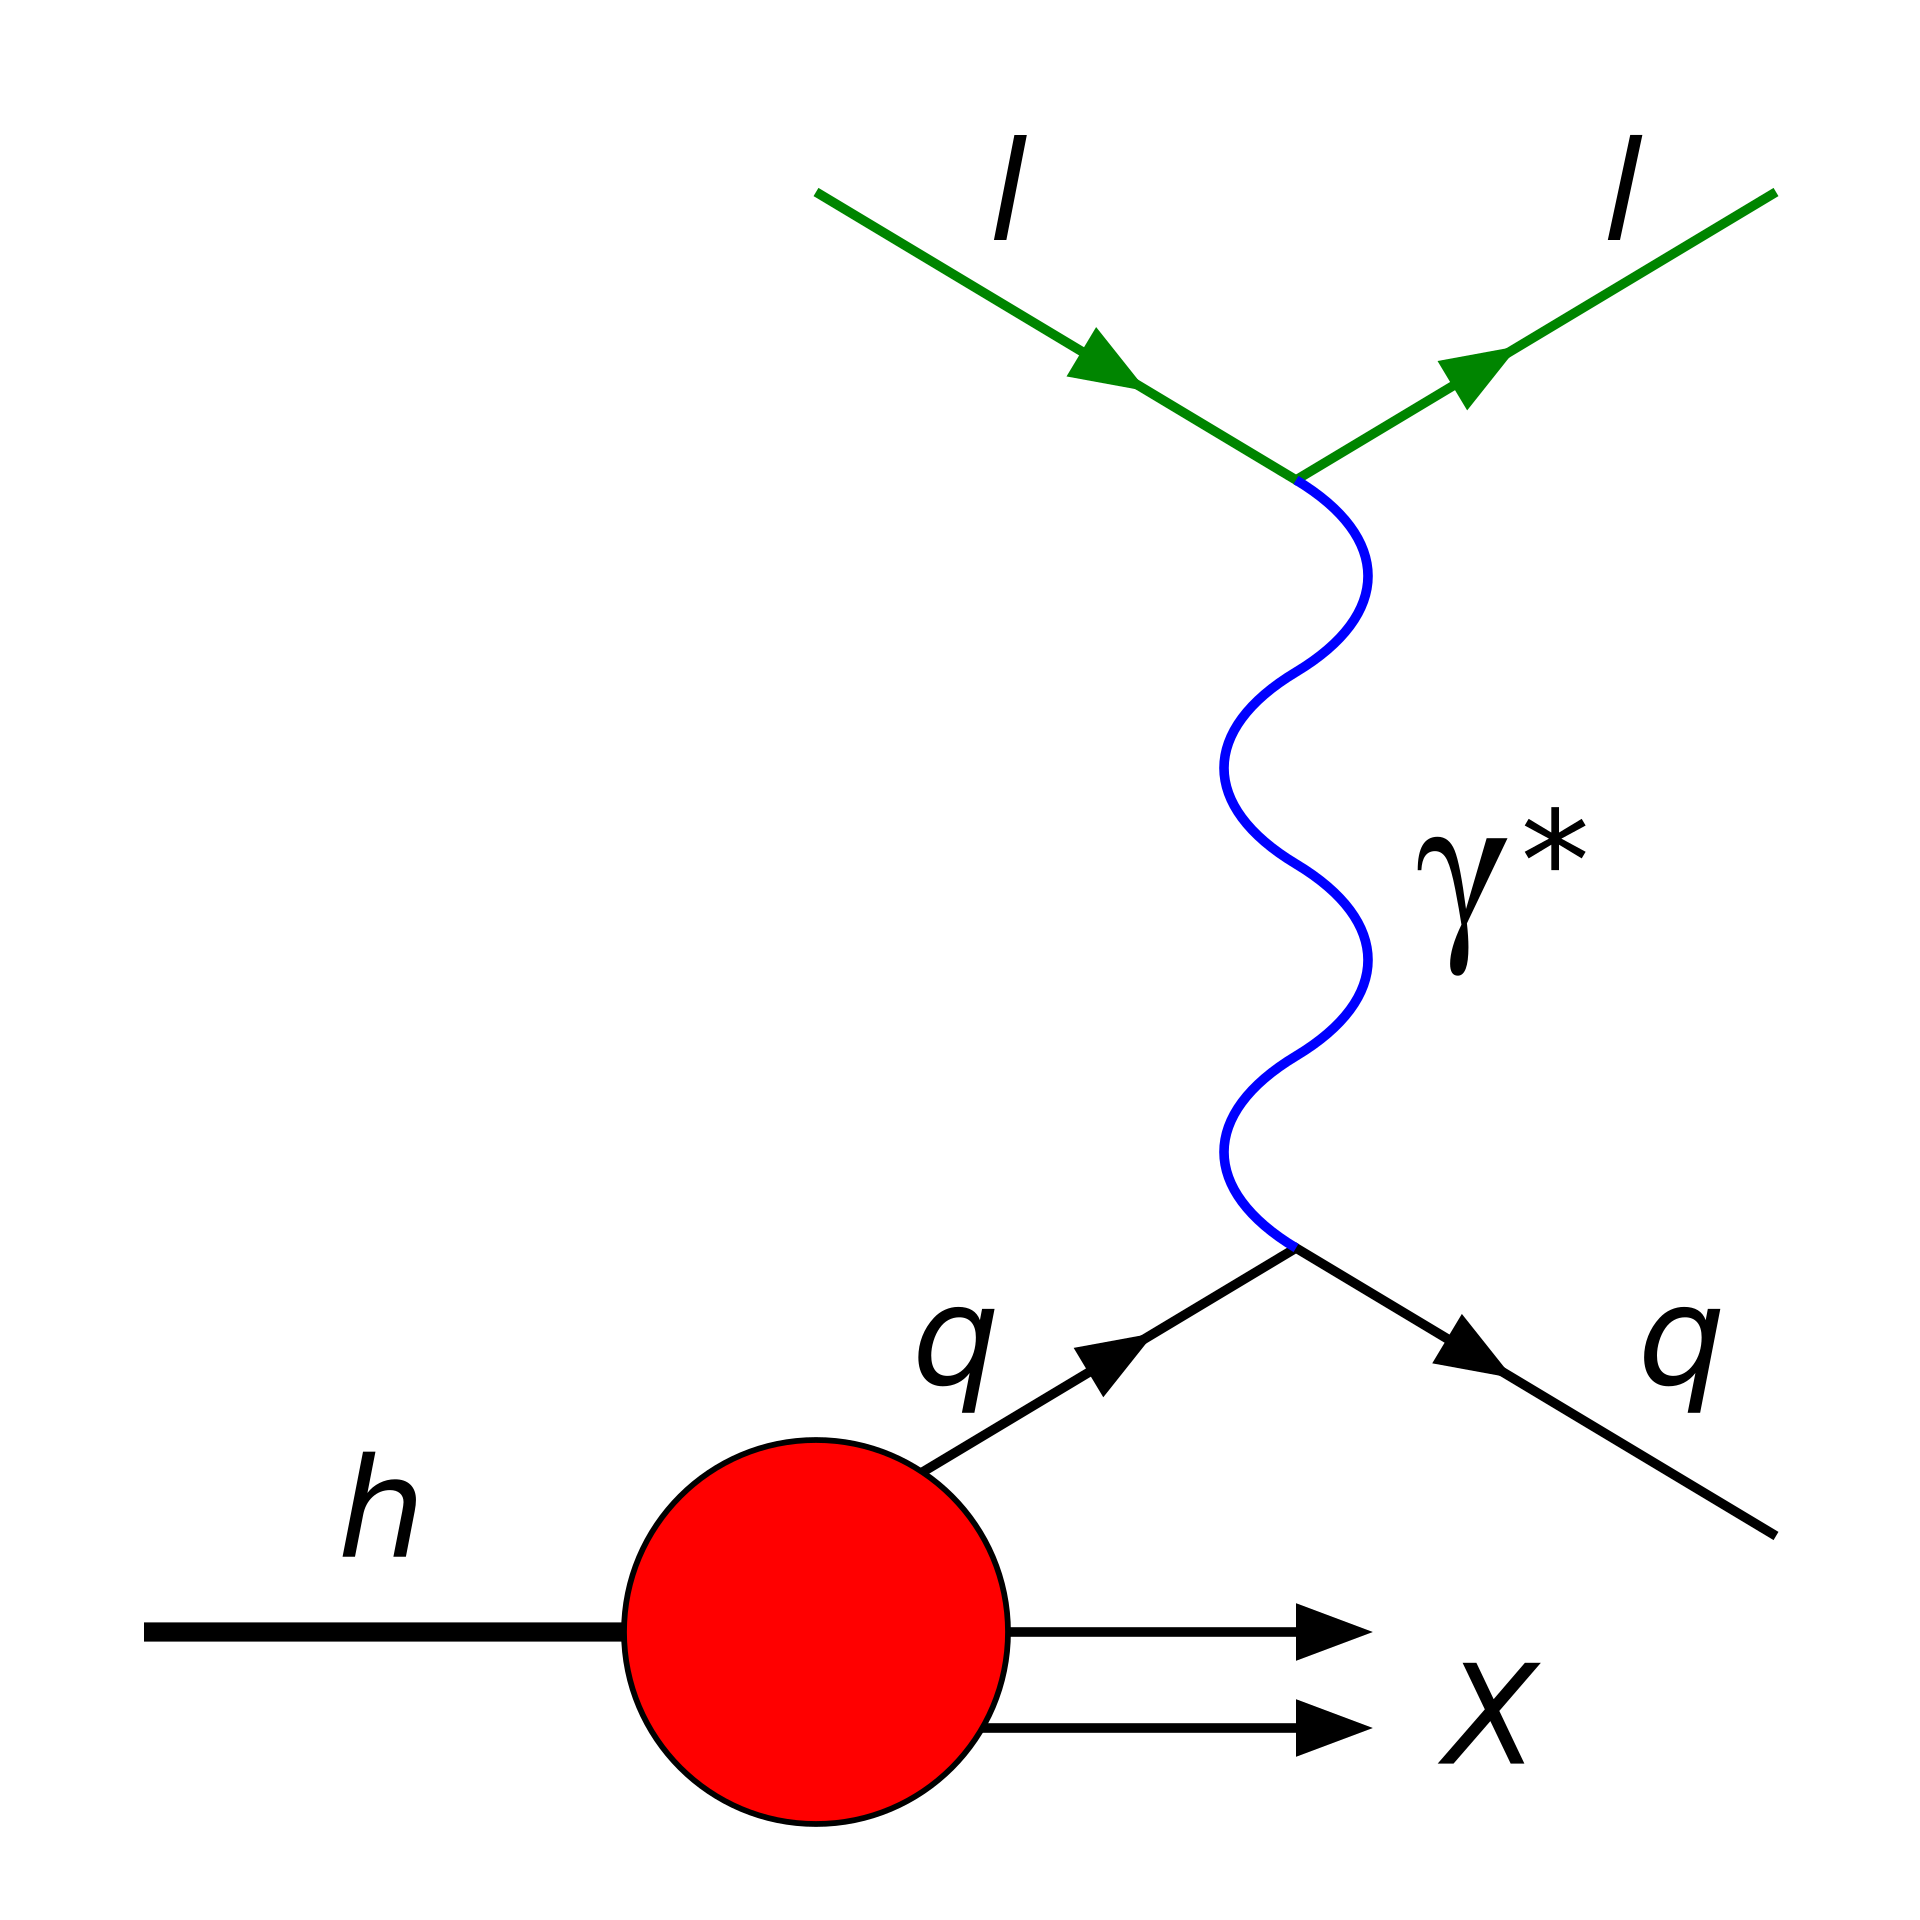
\includegraphics[width=0.3\textwidth]{figures/01-SM-03-SM/qcd/DIS.svg.png}}
	\hspace{1cm}
	\adjustbox{valign=m}{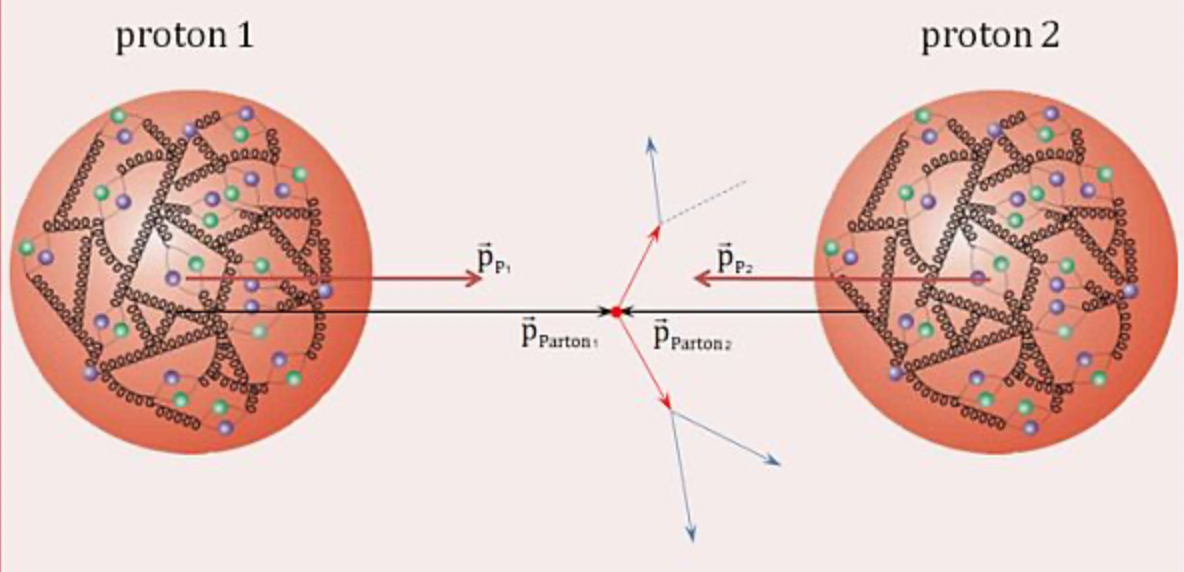
\includegraphics[width=0.45\textwidth]{figures/01-SM-03-SM/qcd/proton-proton.png}}
	\caption{Feynman diagram for deep inelastic scattering, reproduced from Ref.~\cite{enwiki:1240848406} (left) and an illustrative example of proton-proton collisions reproduced from Ref.~\cite{ATLAS:2024protoncollisions} (right).}
	\label{fig:01_sm_qcd_dis}
\end{figure}

\begin{figure}
	\centering
	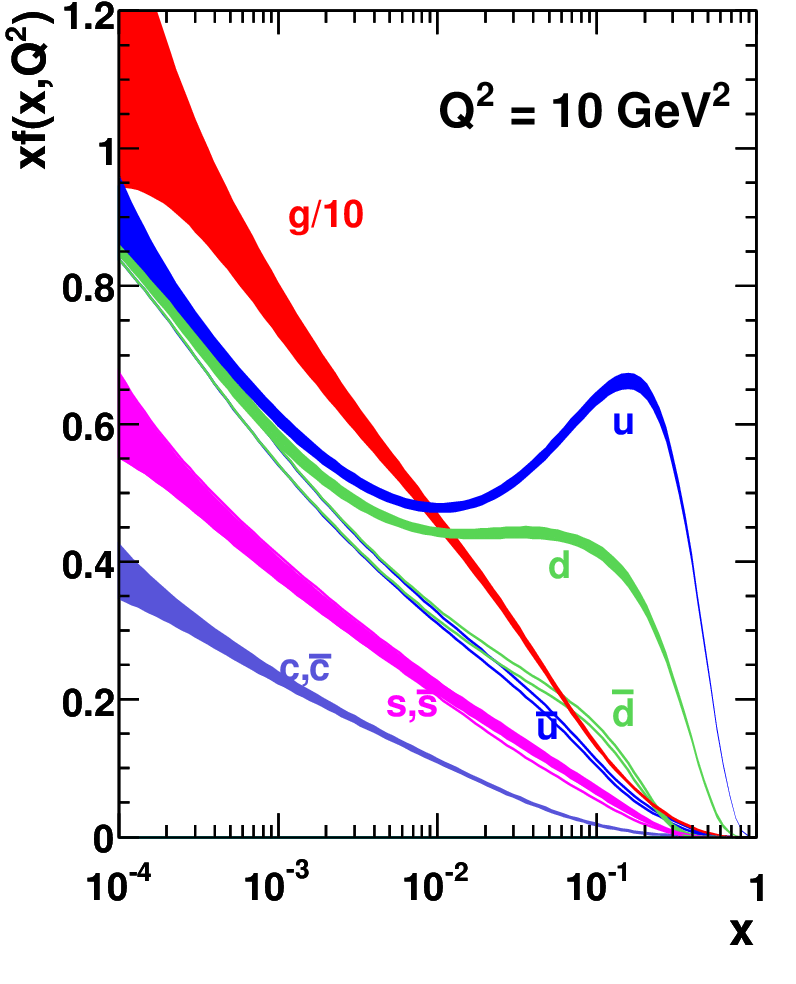
\includegraphics[width=0.5\textwidth]{figures/01-SM-03-SM/qcd/The-MSTW-2008-proton-PDFs.png}
	\caption{PDFs for the proton at $Q^2 = 10 \GeV$, reproduced from Ref.~\cite{Krasny2010}.}
	\label{fig:01_sm_qcd_pdfs}
\end{figure}

\subsubsection{The partonic cross section}

The partonic cross-section $\hat\sigma(Q^2, \mu_r)$ is an important theoretical input for measurements at high energy colliders.
The dependence on $\mu_r$ is perhaps surprising; however, it represents the fact that $\hat\sigma$ is calculated perturbatively: the $\mu_r$ dependence only appears in the highest order term of the expansion.
Indeed, this scale dependence would disappear at infinite order in perturbation theory.
While it may seem a nuisance, in fact, it provides a convenient handle to estimate the \textit{uncertainties} on our theoretical predictions by simply varying $\mu_r$ and $\mu_f$.\footnote{See Ref.~\cite{Salam:2010zt} 4.1 for further discussion.}

One important feature to keep in mind regarding the perturbative calculations for hadron colliders is that the leading order (LO) predictions are often a factor of $\gtrsim 2$ off the higher order next-to-LO (NLO) and next-to-NLO (NNLO) calculations.
This is exemplified in the predictions for \PZ boson production at the LHC, shown in Figure~\ref{fig:01_sm_qcd_qcd_nlo}.
The reason for this, despite $\alpha_s$ being reasonably small ($\approx 0.1$) at the scale for this process $m_Z \simeq 90\GeV$, is simply that the $\mathcal O(\alpha_s)$ corrections have large coefficients~\cite{Salam:2010zt}.
This is why measurements at the LHC relying on LO simulations often multiply the cross-section with an NLO / LO ``K-factor''.

Practically, matrix elements are first calculated as a function of the input and output ``hard particle'' momenta, after which event generator programs such as \MADGRAPH~\cite{Alwall:2014hca} use Monte Carlo (MC) methods to sample events appropriately from the overall phase space.
NLO and NNLO calculations are more complicated and often involve weighting events negatively to represent subtractions at higher orders~\cite{Danziger:2021xvr}.

\begin{figure}[ht]
	\centering
	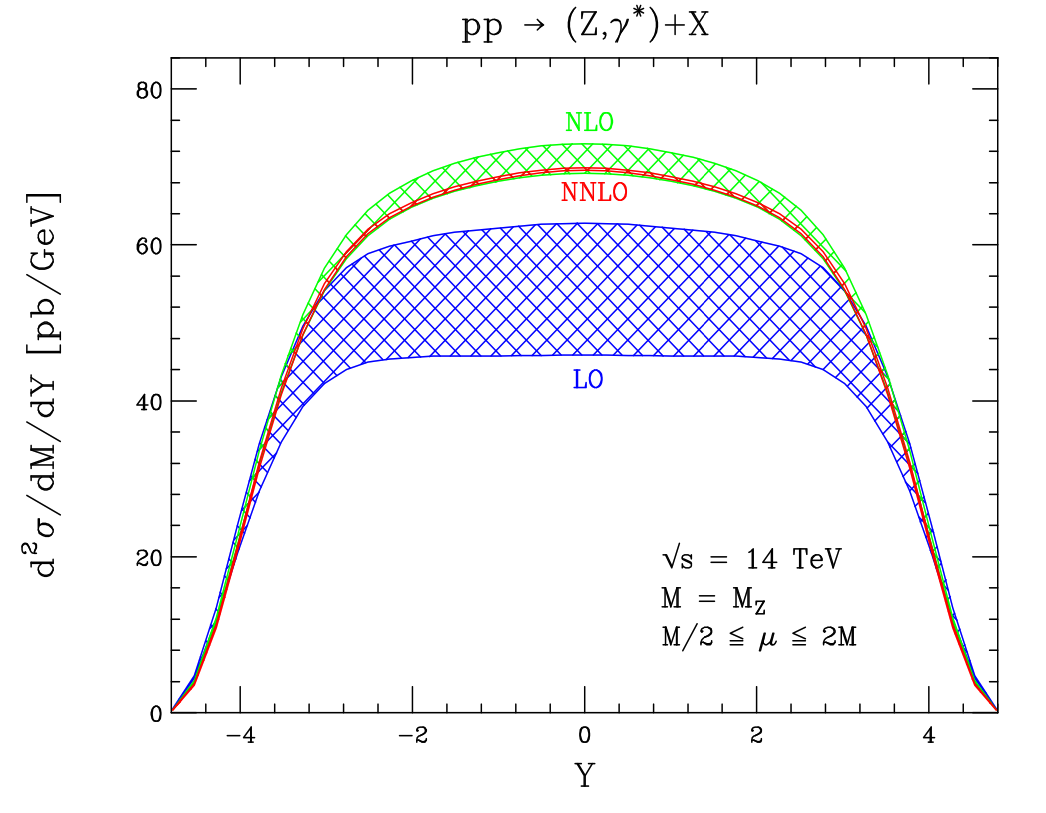
\includegraphics[width=0.7\textwidth]{figures/01-SM-03-SM/qcd/Zxs.png}
	\caption{LO, NLO, and NNLO predictions and uncertainties for $pp$ to Z boson production, differential in rapidity $Y$ at the LHC, reproduced from Ref.~\cite{Anastasiou:2003ds}.}
	\label{fig:01_sm_qcd_qcd_nlo}
\end{figure}


\subsubsection{Parton evolution}

Each parton has a certain probability of radiating another quark or gluon, with a fraction of the original parton's momentum, $z$.
These are called parton splitting functions, $P_{ij}(z)$, depicted in Figure~\ref{fig:01_sm_qcd_splitting}, and can be calculated perturbatively in QCD (see e.g. Ref.~\cite{Salam:2010zt}).
They are then further convolved with PDFs to derive their evolution with the energy scale:
\begin{equation}
	\label{eq:01_sm_qcd_pdf_evolution}
	\frac{\dd f_i(x, Q^2)}{\dd Q^2} = \frac{1}{Q^2} \sum_{j} \int_x^1 \frac{\dd z}{z} f_j(\nicefrac{x}{z}, Q^2) P_{ji}(z).
\end{equation}

Equations~\ref{eq:01_sm_qcd_pdf_evolution} are called the Dokshitzer-Gribov-Lipatov-Altarelli-Parisi (DGLAP) evolution equations, after five physicists who developed them in the 1970s, and are analogous to the renormalization group flows of coupling constants.
The dependence of the PDFs on the energy scale has been confirmed in DIS experiments, which are then also used to fit the parameters of the PDFs, as shown in Figure~\ref{fig:01_sm_qcd_dglap}.

\begin{figure}[ht]
	\centering
	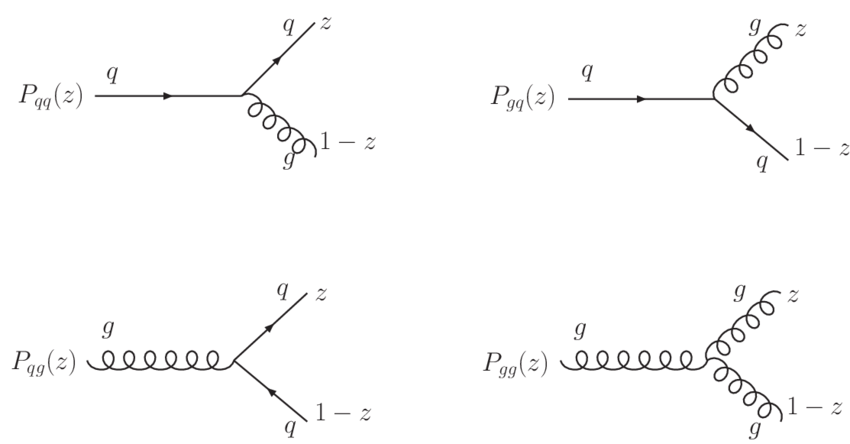
\includegraphics[width=0.9\textwidth]{figures/01-SM-03-SM/qcd/The-splitting-functions.png}
	\caption{The splitting functions for quarks and gluons, reproduced from Ref.~\cite{Kollar:2007TopQuark}.}
	\label{fig:01_sm_qcd_splitting}
\end{figure}

\begin{figure}[ht!]
	\centering
	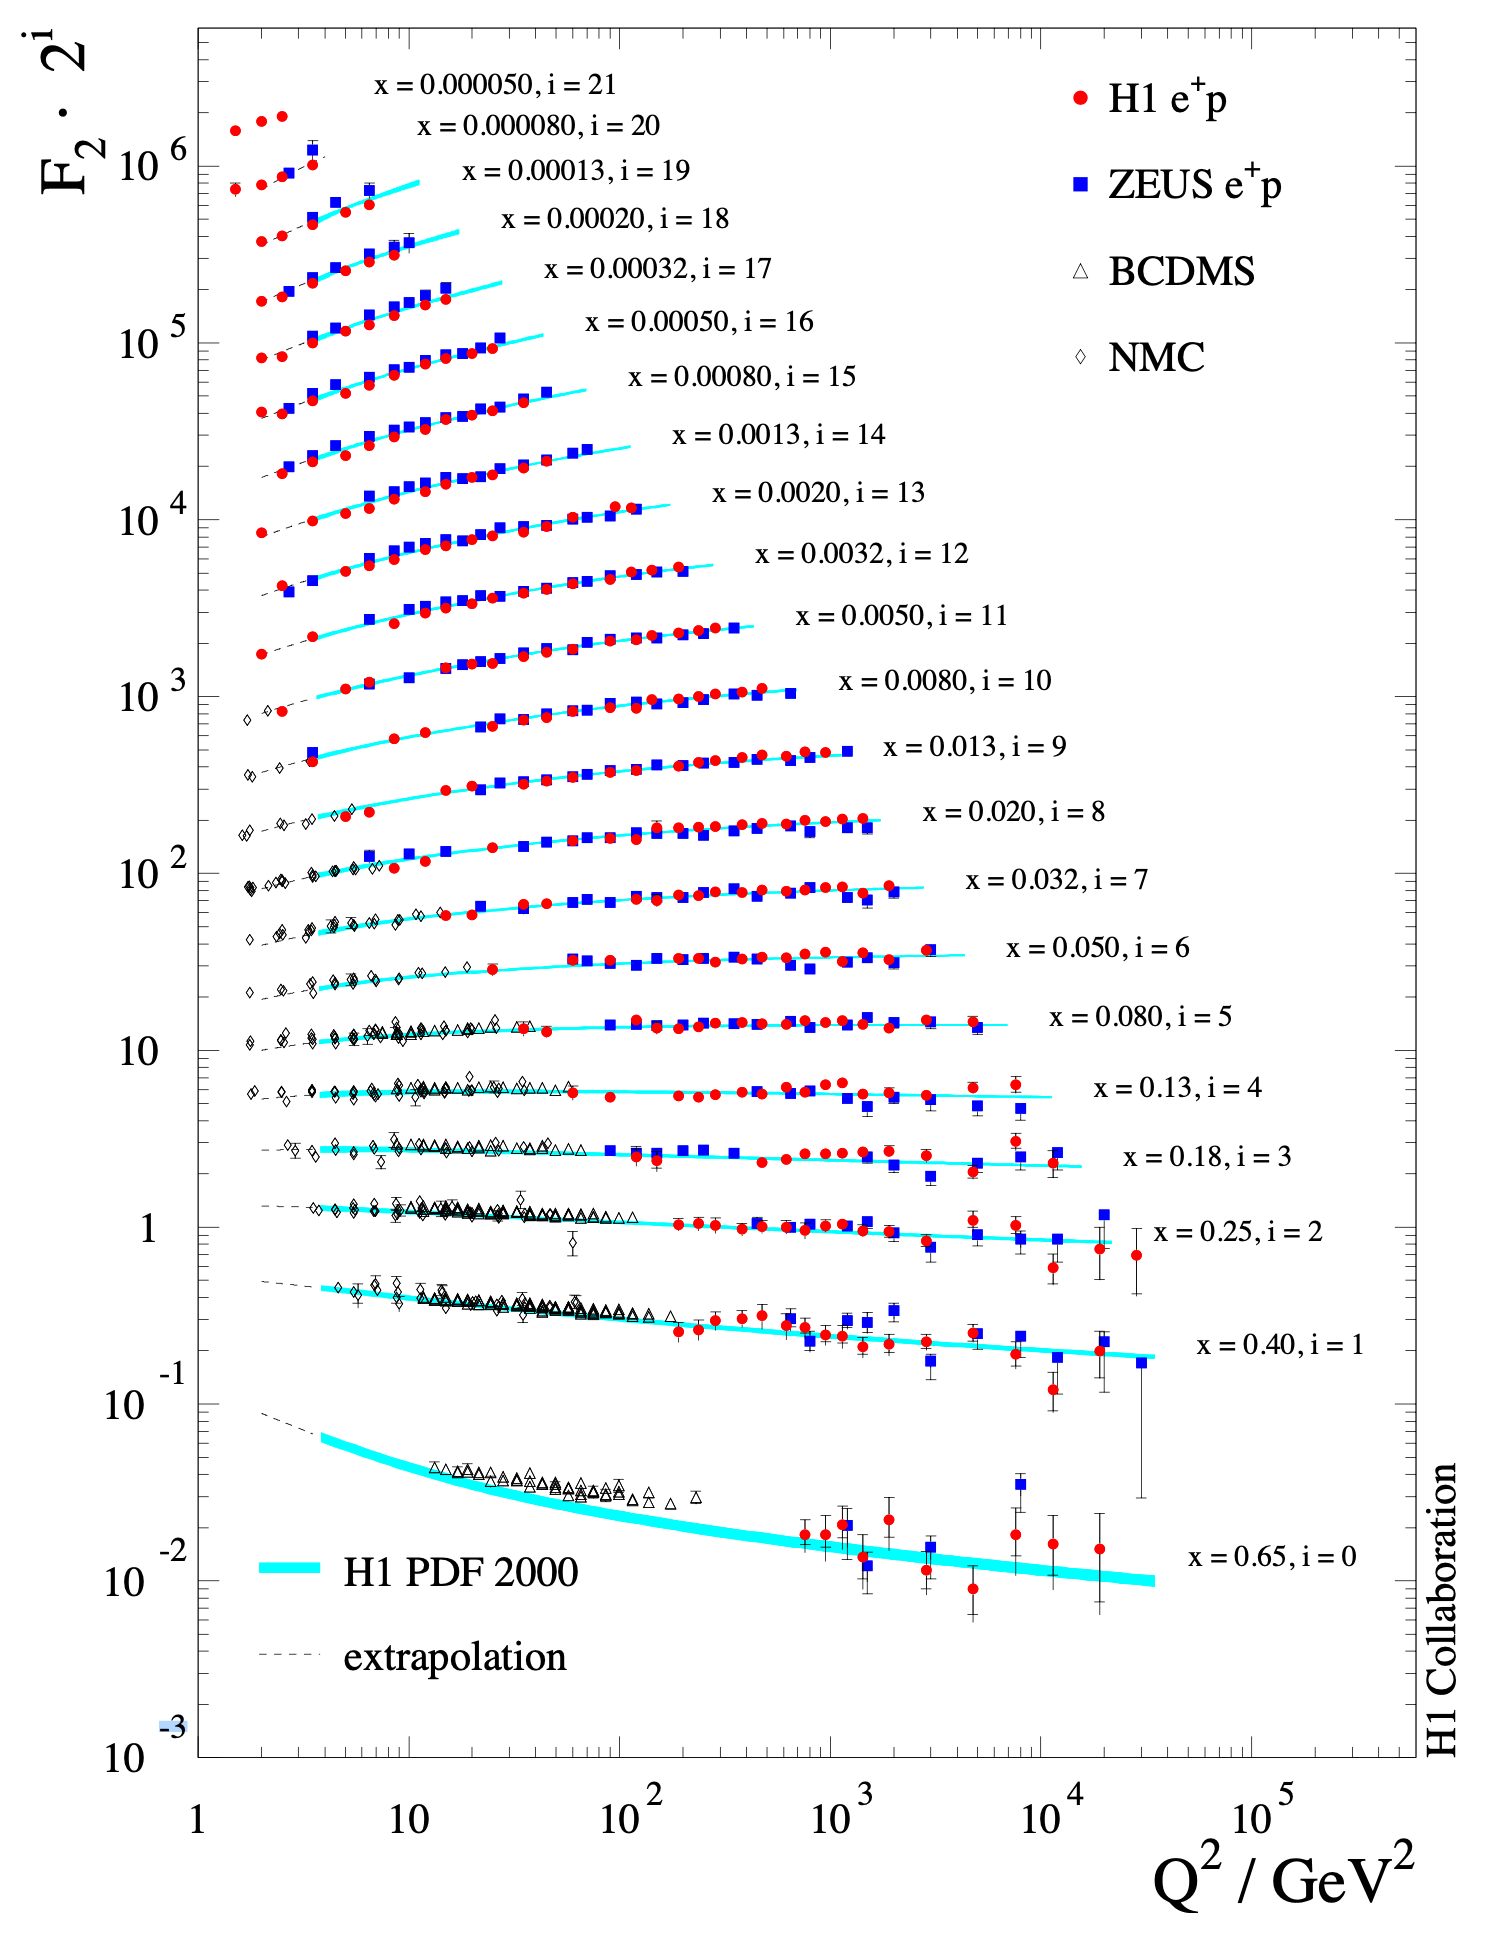
\includegraphics[width=0.75\textwidth]{figures/01-SM-03-SM/qcd/HERA_DIS.png}
	\caption{PDF measurements at different energy scales $Q^2$ and momentum fraction $x$ by the H1 collaboration in DIS experiments, reproduced from Ref.~\cite{Glazov:2007zz}.}
	\label{fig:01_sm_qcd_dglap}
\end{figure}


\subsection{Jets}
\label{sec:01_sm_qcd_jets}

As one may infer from the DGLAP equations (Eq.~\ref{eq:01_sm_qcd_pdf_evolution}), when high energy partons are produced at a collider, they will probabilistically radiate further and further partons --- called \textit{parton showering} --- until they approach the confinement scale and start forming bound hadrons --- called \textit{hadronization}.
For sufficiently high energy initial partons, the resulting hadrons will appear as a collimated spray of particles in the detector, called a \textit{jet} (Figures~\ref{fig:01_sm_qcd_jet_cartoon} and~\ref{fig:01_sm_qcd_jet_event}).

Since quarks and gluons are never observed in isolation, their production can only be inferred by understanding the jets they form.
Moreover, at a hadron collider, the high-energy hadrons continuously radiate partons \textit{before} and \textit{after} the collision as well, with the resulting jets referred to as \textit{initial} and \textit{final state radiation} (ISR and FSR), respectively.
Such jets are by far the most prevalent outputs of collisions at the LHC and, hence, represent a significant background in many measurements and searches, particularly those searching for hadronic final states.

\begin{figure}[ht]
	\centering
	\captionsetup{justification=centering}
	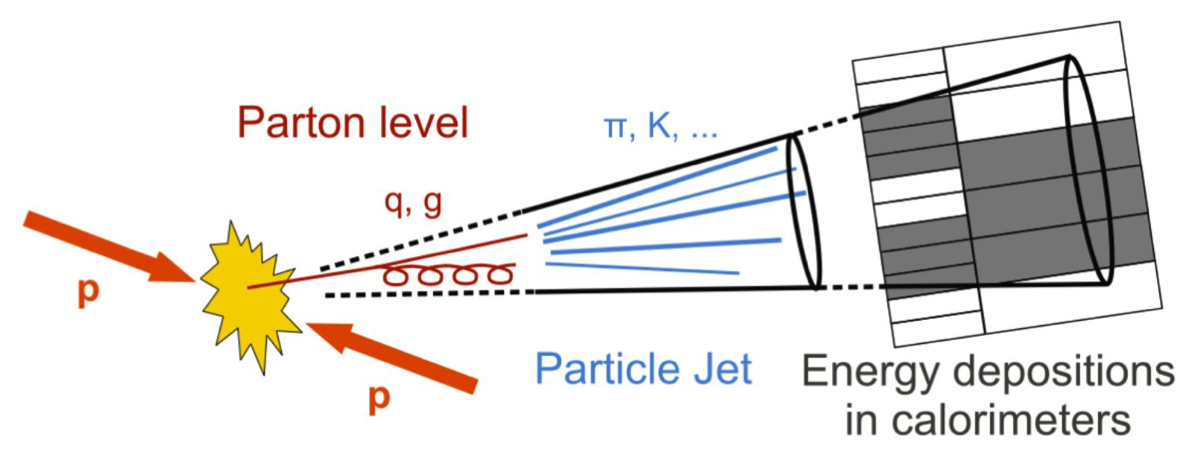
\includegraphics[width=\textwidth]{figures/01-SM-03-SM/qcd/jet_cartoon.png}
	\caption{A cartoon of a jet, reproduced from Ref.~\cite{Kirschenmann:2014vga}.}
	\label{fig:01_sm_qcd_jet_cartoon}
\end{figure}

\begin{figure}[ht]
	\centering
	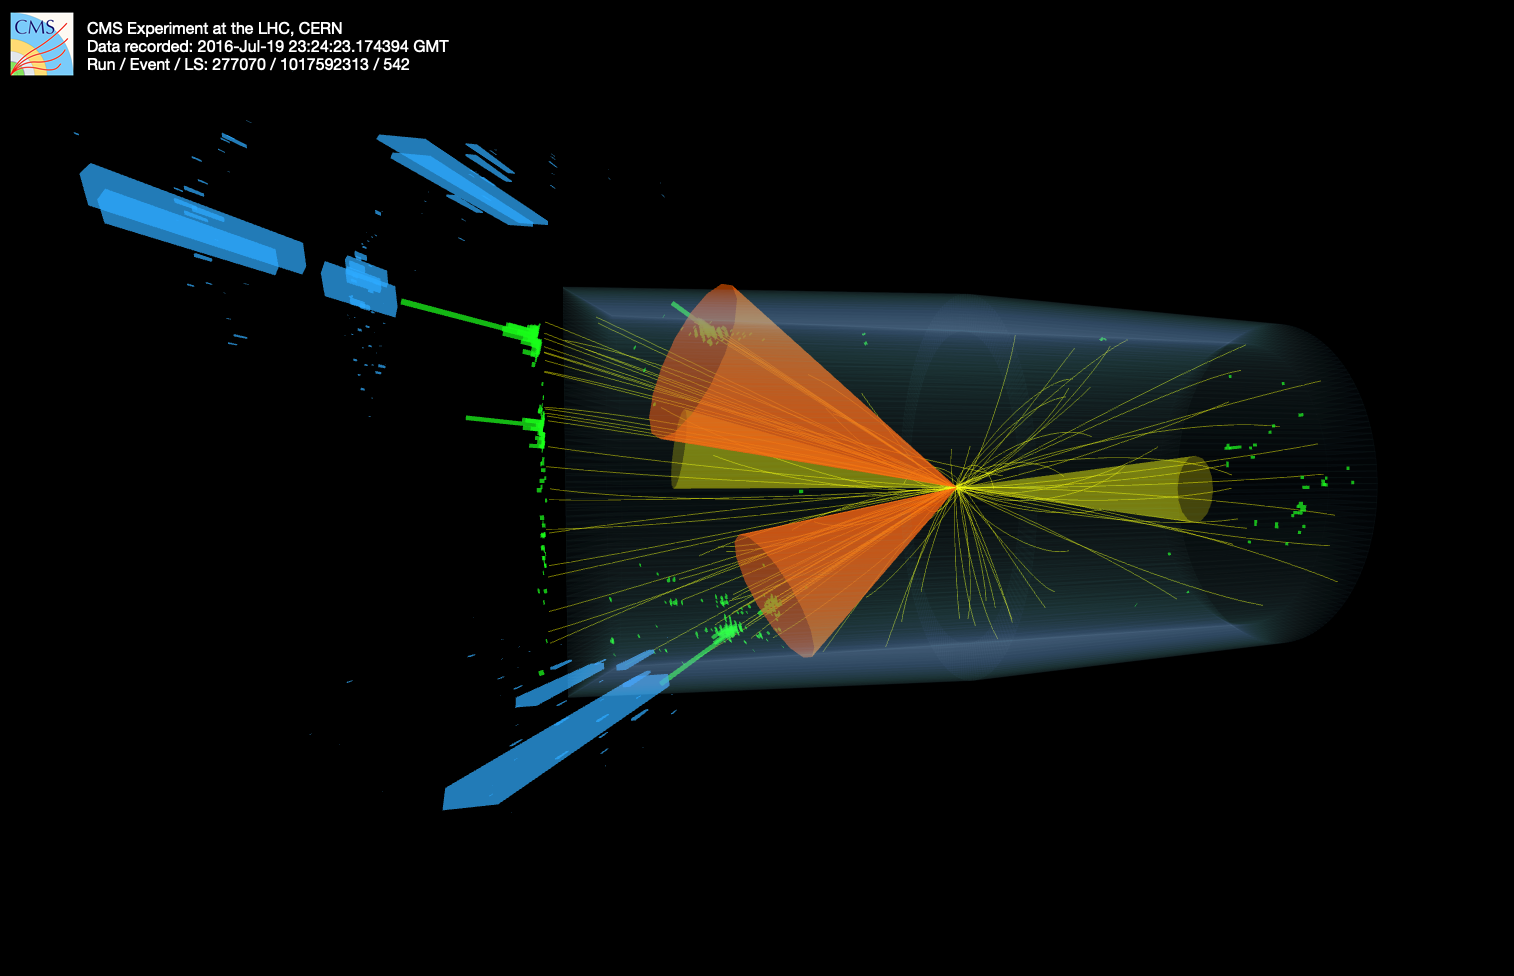
\includegraphics[width=\textwidth]{figures/01-SM-03-SM/qcd/bbww_event.png}
	\caption{An example of real jets in an event collected by CMS and identified in the search described in Chapter~\ref{sec:05_hh}~\cite{Bauerdick:2011zz, CMS:2024les}.
	An interactive version of this event display is available at \url{https://cms3d.web.cern.ch/HIG-23-012/.}}
	\label{fig:01_sm_qcd_jet_event}
\end{figure}


\subsubsection{Parton showering}

Jets can be understood and modeled by factorizing the dynamics.
As above, the parton scattering cross section (referred to as the \textit{hard process} and calculated perturbatively) is separated from the PDFs (measured from data) and their evolution (DGLAP equations).
This evolution is what produces the showering, and is modeled by numerically iterating through $Q^2$ (or, equivalently, through time) and randomly emitting new partons according to the splitting functions via MC sampling.

There are several subtleties involved in this process which numerical parton shower generators, such as \PYTHIA~\cite{Sjostrand:2014zea}, \HERWIG~\cite{Corcella:2000bw}, and \SHERPA~\cite{Sherpa:2019gpd} must account for.
First, the probability of gluon emission diverges in the soft --- i.e., low gluon energy --- and collinear --- small gluon angle with the parent parton --- limits.
Physically, this can be interpreted as the limit of our experimental resolution: at a certain point we cannot resolve two close-by or detect arbitrarily soft particles.

These are known as the \textit{infrared} and \textit{collinear} (IRC) divergences, respectively, and are typically regulated by introducing cut-off energies and angles for emissions (below which we can reasonably argue that perturbation theory is anyway invalid).
These divergences also mean that when analyzing jets in experimental data, care must be taken in defining observables to be \textit{IRC-safe}, meaning that jet clustering algorithms and physical properties derived therein should not be sensitive to arbitrarily soft or collinear emissions.

Another issue is that a naive combination of the hard matrix element and subsequent parton shower calculations may lead to double-counting of emissions, as illustrated in Figure~\ref{fig:01_sm_qcd_doublecounting}.
This necessitates a careful ``matching procedure'', such as the most common MLM scheme~\cite{Alwall:2007fs}, which defines cut-off energy and angular scales to separate the matrix element and parton shower phase spaces.
Other considerations include preserving unitarity, color coherence and color flow, and differences between ISR and FSR (see e.g. Refs.~\cite{Hoche:2014rga, Hoche:2018Lecture}).

\begin{figure}[ht]
	\centering
	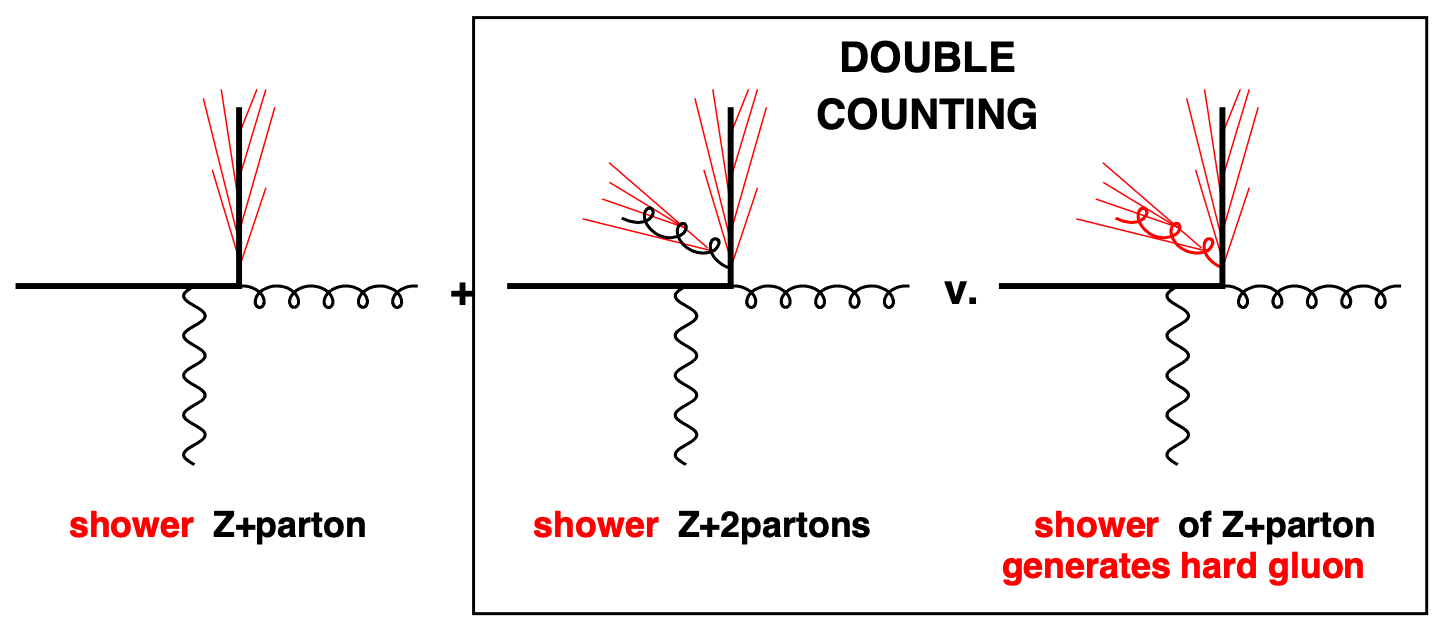
\includegraphics[width=0.8\textwidth]{figures/01-SM-03-SM/qcd/double_counting.png}
	\caption{An illustration of double-counting when combining matrix element predictions (in black) with parton showering algorithms (in red) for $Z+$parton and $Z+$2-parton events, reproduced from Ref.~\cite{Salam:2010zt}.}
	\label{fig:01_sm_qcd_doublecounting}
\end{figure}


\subsubsection{Hadronization}

The final element of the factorized process is hadronization, once the parton shower approaches the confinement scale.
This is a completely nonperturbative process and, hence, like PDFs, we must rely on numerical simulations and experimental measurements.

Lattice QCD simulations, such as those shown in Figure~\ref{fig:01_sm_qcd_fluxtubes}, indicate that in the low energy limit, the effective potential between quarks increases linearly with distance, resembling string tension:
\begin{equation}
	\label{eq:01_sm_qcd_string}
	V(r) = \sigma r,
\end{equation}
where $\sigma$ is the string tension coefficient.
In fact, this analogy can be extended further: above a certain energy, the string appears to ``snap'', in the sense that it becomes possible and energetically more favorable to produce a quark-antiquark pair.

This analogy the basis of the \textit{Lund string model} of hadronization~\cite{Andersson:1983ia}, illustrated in Figure~\ref{fig:01_sm_qcd_lundstring}.
The strong force between the final state partons is modeled as a series of strings stretched between them that probabilistically break into new partons.
Other models are based on clustering partons into color-neutral combinations~\cite{Corcella:2000bw}.

\begin{figure}[ht]
	\centering
	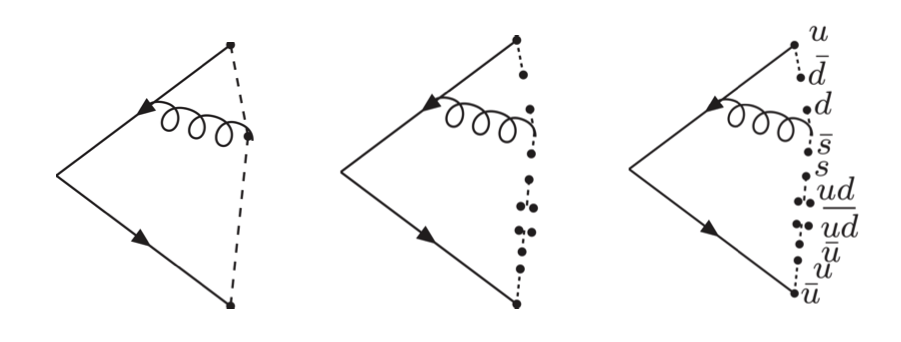
\includegraphics[width=0.6\textwidth]{figures/01-SM-03-SM/qcd/Lund_string.png}
	\caption{An illustration of the Lund string model of hadronization, reproduced from Ref.~\cite{Prestel:2018Lecture}.}
	\label{fig:01_sm_qcd_lundstring}
\end{figure}


% \subsubsection{Defining jets}

% As discussed above, it is important to define jets in an IRC-safe way.

%  - kT class of algorithms, anti-kT is most common \\

% \subsubsection{Identifying jets}

%  - jetnet cartoon \\
%  - quarks vs gluons \\
%  - ``heavy jets'', b jets \\
%  - jet substructure for boosted tops, Higgs \\

% \subsection{Chiral symmetry breaking}


\section{Electroweak interactions}
\label{sec:01_sm_ew}

The weak interaction is the last of the three fundamental forces we discuss in the SM.
Apart from its relatively weak coupling constant (Table~\ref{tab:01_sm_coupling_constants}), it is unique in several ways: (1) it couples only to left-chiral fermions, thereby violating parity ($P$) and charge conjugation ($C$); (2) it is the only force with massive gauge bosons, resulting in short-range interactions; and (3) it is the only force that ``sees'' and can change the flavors of the fermions.
Hence, it is responsible for radioactive decays and the instability of all hadrons and leptons bar the proton and electron.
Its couplings to the different flavors also lead to $CP$-violation, as we discuss in Section~\ref{sec:01_sm_ew_flavor}.

\subsection{Weak interactions}
\label{sec:01_sm_ew_weak}

The first theory of weak interactions was Enrico Fermi's 1933 theory of beta decay~\cite{Fermi:1934hr}: the decay of the neutron to a proton, $n \to p + e^- + \bar\nu_e$, through a four-fermion interaction (Figure~\ref{fig:01_sm_ew_fermi}, left).
Fermi was inspired by Dirac's nascent theory of QED, and using similar perturbative techniques, his theory proved successful in describing weak decays.
The same principle was also applied to other weak decays, such as muon decay (Figure~\ref{fig:01_sm_ew_fermi}, right) and pion decay.

As it turned out, the four-fermion interaction is of mass dimension $6$ and not renormalizable (see Chapter~\ref{sec:01_qft_interactions}), leading to the scattering cross-section diverging at high energies.
This is, of course, because these interactions are in fact mediated by the massive weak $W^\pm$ and $Z$ gauge bosons, which become relevant around their mass scale of $\mathcal O(100\GeV)$.
We now understand the Fermi theory as an effective field theory (EFT) valid for energies much lower than $100 \GeV$, wherein the $W$ and $Z$ boson DoFs can be integrated out and nonrenormalizable interactions are allowed --- they are just suppressed by factors of $(\nicefrac{1}{M_W})^2$.
This suppression is why the weak interaction is so weak, with a coupling constant of $\approx \mathcal O(10^{-6})$ at the mass scale of the proton.

\begin{figure}[ht]
	\centering
	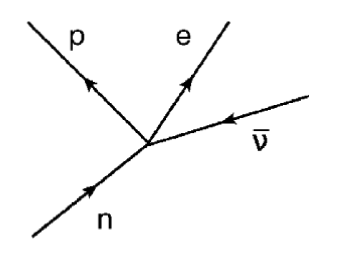
\includegraphics[width=0.25\textwidth]{figures/01-SM-03-SM/ew/beta_decay.png}
	\hspace{1cm}
	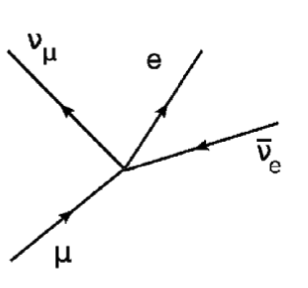
\includegraphics[width=0.2\textwidth]{figures/01-SM-03-SM/ew/muon_decay.png}
	\caption{Feynman diagrams for beta decay (left) and muon decay (right) in Fermi's theory.}
	\label{fig:01_sm_ew_fermi}
\end{figure}

% The discovery of the non-renormalizability of Fermi's theory in the 1950s led to disenchantment with QFT~\cite{WeinbergHistoryQFT}.
% with the advent of Yang-Mills theory, it was proposed that 

The weak interaction is described by an \SU[2] Yang-Mills theory, and is sometimes referred to as quantum flavordynamics (QFD) because of its deep connection to flavor, as we will discuss.
However, ``vanilla'' Yang-Mills theories cannot accommodate massive gauge bosons; hence, it was only after the development of the ABEGHHK (Higgs) mechanism in the 1960s that this description gained traction.
Specifically, Sheldon Glashow, Abdus Salam, Steven Weinberg and others showed that the spontaneous breaking of an \SU[2] $\times$ \UU[1] symmetry to \UU[1] could not only yield massive weak gauge bosons, but also naturally incorporate QED with a massless photon~\cite{Glashow:1959wxa, Salam:1968rm, Weinberg:1967tq}.

This combined \textit{electroweak} theory has been experimentally confirmed in many stages: 
first with the discovery of \textit{neutral currents} involving neutrinos with the Gargamelle bubble chamber at CERN in 1973~\cite{GargamelleNeutrino:1973jyy}, the first evidence for the $Z$ boson (the only neutral boson that couples to neutrinos); 
then with the direct discovery of the $W$ and $Z$ bosons at the Super Proton Synchrotron (SPS) in 1983~\cite{UA1:1983crd, UA1:1983mne, UA2:1983tsx, UA2:1983mlz}, as well as precision measurements of electroweak parameters such as the $W$ and $Z$ masses with the Large Electron-Positron Collider (LEP) in the 1990s; 
and finally with the discovery of the Higgs boson at the LHC in 2012~\cite{CMS:2012qbp, ATLAS:2012yve}, a particle predicted by the ABEGHHK mechanism, and the ongoing measurements of its properties.


\subsection{Before electroweak symmetry breaking}

Electroweak interactions are associated with the $\SU[2]_L \times \UU[1]_Y$ gauge symmetry, which is ``spontaneously broken'' to $\UU[1]_{\text{EM}}$ through the ABEGHHK mechanism during electroweak symmetry breaking (EWSB).\footnote{As discussed in Chapter~\ref{sec:01_qft_higgs}, technically, the gauge symmetry cannot be broken --- what breaks is the associated global symmetry.}
We label the three gauge bosons of $\SU[2]_L$ as $W^1, W^2, W^3$ and of $\UU[1]_Y$ as $B$, with coupling constants $g$ and $g'$, respectively.

The fermions in the SM can be categorized by their representations, or charges, under the three gauge symmetries before EWSB, as in Table~\ref{tab:01_sm_ew_fermions}.
The bold numbers indicate the dimension of the representation under the respective symmetry group, while the regular numbers are the charges under the $\UU[1]_Y$ group --- referred to as their \textit{hypercharge}, $Y$.

\begin{table}[ht]
	\renewcommand{\arraystretch}{1.5}
	\centering
	\begin{tabular}{c|ccc}
		 & $\UU[1]_Y$ & $\SU[2]_L$ & $\SU[3]_C$ \\
		\midrule
		$Q_L$ & $+ \nicefrac{1}{6}$ & $\mathbf{2}$ & $\mathbf{3}$ \\
		$L_L$ & $- \nicefrac{1}{2}$ & $\mathbf{2}$ & $\mathbf{1}$ \\
		$u_R$ & $+ \nicefrac{2}{3}$ & $\mathbf{1}$ & $\mathbf{3}$ \\
		$d_R$ & $- \nicefrac{1}{3}$ & $\mathbf{1}$ & $\mathbf{3}$ \\
		$e_R$ & $-1$ & $\mathbf{1}$ & $\mathbf{1}$ \\
		$\nu_R$ (?) & $0$ & $\mathbf{1}$ & $\mathbf{1}$ \\
		$H$ & $+ \nicefrac{1}{2}$ & $\mathbf{2}$ & $\mathbf{1}$ \\
	\end{tabular}
	\vspace{2mm}
	\caption{The representations and charges of fermionic and scalar fields in the SM under the $\UU[1]_Y$, $\SU[2]_L$, and $\SU[3]_C$ gauge symmetries. 
	The right-handed neutrino is included here for completeness but has not been experimentally confirmed.}
	\label{tab:01_sm_ew_fermions}
\end{table}

The weak interactions specifically are associated with the $\SU[2]_L$ gauge symmetry, and their key characteristic is that they violate parity: they only couple to left-handed fermions and right-handed antifermions (hence, the subscript $L$).
Specifically, the left-handed quarks ($u_L$ and $d_L$) and leptons ($\nu_L$ and $e_L$) reside in $\SU[2]_L$ doublets:
\begin{equation}
	\label{eq:01_sm_ew_doublets}
	Q_L = \begin{pmatrix} u_L \\ d_L \end{pmatrix}, \quad L_L = \begin{pmatrix} \nu_L \\ e_L \end{pmatrix},
\end{equation}
while right-handed fermions live in the trivial representation.
The $L$ and $R$ subscripts indicate left- and right-chiral Weyl spinors, respectively.
Note that there are actually three generations of fermions, which we index as $u^i$ for $i = 1, 2, 3$; however, before EWSB, there is no distinction between them as they are all massless.
Often, we will omit this index when the properties across generations are identical.

The SM also contains a scalar, \SU[2]-doublet ``Higgs'' field $H$, which is listed in Table~\ref{tab:01_sm_ew_fermions} as well.
Its dynamics are governed by the Lagrangian:
\begin{equation}
	\label{eq:01_sm_ew_higgs_lagrangian}
	\mathcal{L}_\mathrm{Higgs} = (D_\mu H)^\dagger (D^\mu H) - \lambda (H^\dagger H - \frac{v^2}{2})^2,
\end{equation}
where $v$ is a constant and
\begin{equation}
	\label{eq:01_sm_ew_higgs_derivative}
	D_\mu H = \left[\partial_\mu - igW_\mu - \frac{i}{2} g' B_\mu\right]H
\end{equation}
is the covariant derivative of $H$.
The potential resembles the sombrero potential from Figure~\ref{fig:01_qft_higgs_potential}, but with a 2D rather than 1D complex field.

The Higgs field is able to couple to the fermions without violating gauge symmetry through Yukawa interactions.
The most general possible Yukawa terms are $3 \times 3$ matrices across the three generations.
\begin{equation}
	\label{eq:01_sm_ew_yukawa}
	\mathcal{L}_\mathrm{Yukawa} = -y^d_{ij} \bar{Q}^i_L H d^j_R - y^u_{ij} \bar{Q}^i_L \tilde H u^j_R - y^e_{ij} \bar{L}^i_L H e^j_R - y^\nu_{ij} \bar{L}^i_L \tilde H \nu^j_R + \text{h.c.},
\end{equation}
where $\tilde H = i\sigma_2 H^\dagger$ is the charge-conjugated Higgs field, $i$ and $j$ index the three generations of fermions, $y^d_{ij}$ are the Yukawa coupling constant matrices, and h.c. denotes the Hermitian conjugate of all the preceding terms.

The Higgs field contracts with the fermionic left-handed \SU[2]-doublets to produce an \SU[2]-singlet, while the quark fields contract with each other to form \SU[3]-singlets.
One can also check that through our clever choice of $H$ vs. $\tilde H$, the total hypercharge of each term is $0$.
Thus, each Yukawa term is independently gauge invariant.
% Finally, the quark fields contract with each other to form \SU[3]-singlets as well.

The overall electroweak Lagrangian is:
% \begin{equation}
\begin{multline}
	\label{eq:01_sm_ew_lagrangian}
	\mathcal{L}_\mathrm{EW} = -\frac{1}{4} W^a_{\mu\nu} W^{a\mu\nu} - \frac{1}{4} B_{\mu\nu} B^{\mu\nu} \\ 
	+ \bar{Q}_L i \slashed{D} Q_L + \bar{L}_L i \slashed{D} L_L + \bar{u}_R i \slashed{D} u_R + \bar{d}_R i \slashed{D} d_R + \bar{e}_R i \slashed{D} e_R \\
	+ \mathcal{L}_\mathrm{Higgs} + \mathcal{L}_\mathrm{Yukawa},
\end{multline}
% \end{equation}
Note that without EWSB, not only are all the gauge bosons of the theory massless, but so are the fermions:
the usual fermionic mass terms of the form $m u_L u_R$ violate the $\SU[2]_L$ gauge symmetry.
% Because of this, there is also no distinction so far between the three generations of fermions.
As we will see, the ABEGHHK mechanism is what generates masses for all the fermions, through the Higgs Yukawa couplings, as well as the three weak gauge bosons.

\subsection{Electroweak symmetry breaking}
\label{sec:01_sm_ew_ewsb}

EWSB occurs when the Higgs field spontaneously breaks the global $\SU[2]_L \times \UU[1]_Y$ symmetry by moving to a ground state of the potential.
Without loss of generality, we can choose this ground state to be:
\begin{equation}
	\label{eq:01_sm_ew_higgs_vev}
	\langle H \rangle = \frac{1}{\sqrt{2}} \begin{pmatrix} 0 \\ v \end{pmatrix},
\end{equation}
where $\langle H \rangle$ is the vacuum expectation value (VEV) of the Higgs field.
As before, we can parametrize the fluctuations around this ground state as:
\begin{equation}
	\label{eq:01_sm_ew_higgs_fluctuations}
	H = e^{i \xi^A(x)T^A}
	\frac{1}{\sqrt{2}} \begin{pmatrix} 0 \\ v + h(x) \end{pmatrix},
\end{equation}
where $h$ is a real scalar field, $T^A$ are three generators of the broken $\SU[2]_L \times \UU[1]_Y$ symmetry, and $\xi^A$ are the corresponding Goldstone bosons.

The ABEGHHK mechanism for gauge theories effectively involves the original gauge bosons absorbing these Goldstone bosons, thereby acquiring mass (see Chapter~\ref{sec:01_qft_higgs}).
This can be equivalently thought of as simply a convenient choice of gauge in which $\xi^A(x) = 0$.
In the end, after some algebra, the gauge $+$ Higgs sector of the electroweak Lagrangian after EWSB looks like:
\begin{multline}
	\label{eq:01_sm_ew_gauge_lagrangian}
	\mathcal{L}_\mathrm{GH} = -\frac{1}{4} W^a_{\mu\nu} W^{a\mu\nu} - \frac{1}{4} B_{\mu\nu} B^{\mu\nu} + \frac{1}{2}\partial_\mu h \partial^\mu h - \underbrace{\lambda h^2 \left(v + \frac{h}{2}\right)^2}_{\equiv V(h)} \\
	+ \frac{1}{8} (v + h)^2 \left[g^2 (W^1_\mu)^2 + g^2 (W^2_\mu)^2 + (g W^3_\mu - g' B_\mu)^2\right],
\end{multline}
where $V(h)$ is the new Higgs potential.

We now have mass terms for three gauge, as well as the Higgs, bosons.
As always, we are free to define the gauge boson fields as we wish, and it turns out the most convenient choice is:
\begin{equation}
	\label{eq:01_sm_ew_gauge_fields}
	\begin{split}
		W^\pm_\mu &= \frac{1}{\sqrt{2}} (W^1_\mu \mp i W^2_\mu), \\
		Z_\mu &= \frac{1}{\sqrt{g^2 + g'^2}} (g W^3_\mu - g' B_\mu), \\
		A_\mu &= \frac{1}{\sqrt{g^2 + g'^2}} (g' W^3_\mu + g B_\mu).
	\end{split}
\end{equation}
It is conventional to define the \textit{Weinberg} or \textit{weak mixing angle} $\theta_W$:
\begin{equation}
	\label{eq:01_sm_ew_weinberg}
	\cos \theta_W = \frac{g}{\sqrt{g^2 + g'^2}}, \quad \sin \theta_W = \frac{g'}{\sqrt{g^2 + g'^2}},
\end{equation}
to simplify the forms of $Z$ and $A$ above:
\begin{equation}
	\label{eq:01_sm_ew_z_a}
	\begin{split}
		Z_\mu &= W^3_\mu \cos \theta_W - B_\mu \sin \theta_W, \\
		A_\mu &= W^3_\mu \sin \theta_W + B_\mu \cos \theta_W.
	\end{split}
\end{equation}
Experimentally, we have determined the free parameters of this theory to be:
\begin{equation}
	\label{eq:01_sm_ew_constants}
		v \approx 250\GeV, \quad \lambda \approx 0.35, \quad g \approx 0.64, \quad g' \approx 0.34 \quad \Rightarrow \quad \sin^2 \theta_W \approx 0.223,
\end{equation}
at an energy scale of the $Z$ boson mass.

The Lagrangian can hence be written as:
\begin{multline}
	\label{eq:01_sm_ew_gauge_lagrangian_weinberg}
		\mathcal{L}_\mathrm{GH} = -\frac{1}{4} W^+_{\mu\nu} W^{-\mu\nu} - \frac{1}{4} Z_{\mu\nu} Z^{\mu\nu} - \frac{1}{4} F_{\mu\nu} F^{\mu\nu}
		+  m_W^2 W^+_\mu W^{-\mu} + \frac{1}{2} m_Z^2 Z_\mu Z^\mu \\
		+ \frac{2 m_W^2}{v} h W^+_\mu W^{-\mu} + \frac{m_Z^2}{v} h Z_\mu Z^\mu + \frac{m_W^2}{v^2} h^2 W^+_\mu W^{-\mu} + \frac{m_Z^2}{4v^2} h^2 Z_\mu Z^\mu \\
		+ \frac{1}{2}\partial_\mu h \partial^\mu h - m_h^2 h^2 - \lambda v h^3 - \frac{1}{4} \lambda h^4,
\end{multline}
where
\begin{equation}
	\label{eq:01_sm_ew_masses}
	m_W = \frac{1}{2} vg \approx 80 \GeV, \quad m_Z = \frac{1}{2} v \sqrt{g^2 + g'^2} \approx 91 \GeV, \quad m_h = \sqrt{2\lambda} v \approx 125 \GeV.
\end{equation}

Note that in addition to the gauge-boson self-interactions, the Higgs field also has a trilinear ($\lambda v h^3$) and quartic ($\nicefrac{1}{4} \lambda h^4$) self-interaction terms.
While some manner of EWSB has been confirmed experimentally through the discovery of the Higgs boson, its full nature, and the full form of the Higgs potential, can only be determined through measurements of these terms.
The trilinear self-coupling, in particular, can be accessed at the LHC through pair production of the Higgs boson, as we will discuss in Section~\ref{sec:01_higgs}.
Higgs pair production also allows exclusive access to the quartic $hhVV$ couplings, where $V$ is a weak gauge boson.

\subsubsection{The photon and re-emergence of Dirac spinors}

$A_\mu$ corresponds to the one unbroken symmetry of the original $\SU[2]_L \times \UU[1]_Y$ group.
In terms of the original generators --- three $T^A$s for $\SU[2]_L$ and one $Y$ for $\UU[1]_Y$ --- $A_\mu$ corresponds to linear combination $Q = T^3 + Y$.
This is the massless photon field, with the gauge group $\UU[1]_\mathrm{EM}$.

The eigenvalue of $Q$ for each fermion corresponds to their electric charge under this group.
For the $\SU[2]_L$-singlet fields, $T_3$ has no value and hence $Q = Y$, while for the doublets, $T_3$ has eigenvalues $\pm \nicefrac{1}{2}$ for the upper and lower components, respectively: e.g. for $u_L$, $Q = \nicefrac{1}{2} + \nicefrac{1}{6} = \nicefrac{2}{3}$ and for $e_L$, $Q = -\nicefrac{1}{2}-\nicefrac{1}{2} = 1$.
In the end, we see that the left- and right-chiral fermion field pairs have the same charge under this remaining unbroken symmetry, so they can again form Dirac spinors:
\begin{equation}
	\label{eq:01_sm_ew_dirac}
	\psi_u = \begin{pmatrix} u_L \\ u_R \end{pmatrix}, \quad \psi_d = \begin{pmatrix} d_L \\ d_R \end{pmatrix}, \quad \psi_e = \begin{pmatrix} e_L \\ e_R \end{pmatrix}, \quad \psi_\nu = \begin{pmatrix} \nu_L \\ \nu_R \end{pmatrix},
\end{equation}
times three for each generation.

Each Weyl spinor pair interacts identically with the photon and gluons but the $W$ and $Z$ bosons continue to couple only to the left-handed components.
For example the $W^+$--fermion coupling is:
\begin{equation}
	\label{eq:01_sm_ew_w_coupling}
	\mathcal{L}_{W^+f} = -\frac{g}{\sqrt{2}} W^+_\mu \underbrace{\left(\bar{u}_L \bar\sigma^\mu d_L + \bar{\nu}_L \bar\sigma^\mu e_L\right)}_{\equiv J^+_\mu},
\end{equation}
where $J^+_\mu$ is called the weak charged current.
%  (this interaction is hence also referred to as a weak charged current interaction).
In terms of Dirac spinors, this can be written using the projection operator (Eq.~\ref{eq:01_qft_spinors_chiral_projection}):
\begin{equation}
	\label{eq:01_sm_ew_w_coupling_dirac}
	\mathcal{L}_{W^+f} = -\frac{g}{\sqrt{8}} W^+_\mu \left(\bar{\psi}_u \gamma^\mu (1 - \gamma_5) \psi_d + \bar{\psi}_\nu \gamma^\mu (1 - \gamma_5) \psi_e\right).
\end{equation}
Recall that $\bar\psi \gamma^\mu \psi$ is a Lorentz vector, while $\bar\psi \gamma^\mu \gamma_5 \psi$ is a pseudo- or axial-vector, so the weak current is effectively an axial vector subtracted from a vector.
Indeed, historically, the weak interaction was referred to as ``V-A'' theory.

\subsubsection{A hierarchy problem}

Generally, if we encounter a new energy scale in nature, we are either able to connect it in some way to an existing scale or a (broken) symmetry of the theory.
For example, the mass of the proton $\sim 1\GeV$ is based on the QCD confinement scale $\Lambda_{\text{QCD}} \sim 200\MeV$, which in turn is related to the Planck scale $\Lambda_{\text{Planck}} \sim 10^{19}\GeV$ through dimensional transmutation.
The mass of the pion on the other hand, $\approx 140\MeV$, is a consequence of chiral symmetry breaking in QCD.
Physicists such as Dirac and Gell-Mann have in fact proposed these criteria as a principle of ``naturalness'' for physical theories~\cite{Dirac:1938mt, Gell-Mann:1956iqa}.

There are many examples of mysterious energy scales appearing experimentally, which were either later rationalized or in fact even used to correctly predict new physics, such as the prediction of the charm quark mass based on the small mass difference between the $K_L^0$ and $K_S^0$ mesons.
The electroweak energy scale of $\approx 100\GeV$ is one such example which has yet to be explained.

A common way of expressing the problem is based on the Higgs mass: if we believe the SM to be an EFT valid up to some energy scale $\Lambda$, and if we have \textit{a priori} no other energy scale to which to tie the Higgs mass, then we expect higher order corrections to its bare mass to be of order $\Lambda$.
For example, if there is no new physics up to the Planck scale, then we are left with a bare mass and correction both of order $10^{19} \GeV$.
The fact that the actual mass is $125 \GeV$ implies a cancellation between the two, or \textit{finetuning}, at a $\nicefrac{125}{10^{19}} \approx 10^{-15}\%$ level.
This is considered highly ``unnatural'' and is called a \textit{hierarchy problem}, perhaps hinting at new physics.

One possibility is that $\Lambda$ is in fact on the order of the Higgs mass, and we are simply yet to find the new degrees of freedom at this $\mathcal O(100\GeV)$ scale.
Or, if we accept a higher level of finetuning, e.g. at the $10\%$ or $1\%$ levels, $\Lambda$ can be pushed up further to $1$--$10\TeV$.
Effectively, we can invert the hierarchy problem into setting a bound on new physics!

Another solution is the existence an underlying (approximate) symmetry of nature ``protecting'' the Higgs mass from higher order corrections, similar to the chiral symmetry for the pion mass.
The most promising candidate is \textit{supersymmetry}, postulating an additional global symmetry between bosons and fermions~\cite{Wess:1992cp}.
Both these solutions possibly hint at an extended scalar sector, with either another Higgs doublet or new scalar singlets, for example, through the minimal supersymmetric extension of the SM (MSSM)~\cite{Craig:2013hca} or based on two-real-scalar-singlet models~\cite{Robens:2019kga}.
This is one motivation behind the search for new Higgs bosons described in this dissertation.
% The fact that we have found no hints for either explanation to the hierarchy problem at the LHC in 10 years, however, has raised concerns regarding whether it is a problem at all, and not simply a fact of nature (AKA the anthropic principle)~\cite{Weinberg:1987dv}.
A more detailed, pedagogical discussion of naturalness can be found in e.g. Nathaniel Craig's IAS lectures~\cite{Craig:2017Lecture}.


\subsection{Fermion masses and flavor}
\label{sec:01_sm_ew_flavor}

After EWSB, we have
\begin{equation}
	\label{eq:01_sm_ew_higgs_tilde}
	H = \frac{1}{\sqrt{2}} \begin{pmatrix} 0 \\ v + h \end{pmatrix}, \quad
	\tilde H = \frac{1}{\sqrt{2}} \begin{pmatrix} v + h \\ 0 \end{pmatrix},
\end{equation}
which yields the following Yukawa Lagrangian:
\begin{equation}
	\label{eq:01_sm_ew_yukawa_after}
		\mathcal{L}_\mathrm{Yukawa} = -\frac{1}{\sqrt{2}}(v + h) \left[y^d_{ij} \bar d^i_L d^j_R + y^u_{ij} \bar u^i_L u^j_R + y^e_{ij} \bar e^i_L e^j_R + y^\nu_{ij} \bar \nu^i_L \nu^j_R\right] + \text{h.c.}.
\end{equation}
Again, we are free to redefine fields and can choose a basis for all the fermion fields in which the Yukawa matrices are diagonal:
\begin{equation}
	\label{eq:01_sm_ew_yukawa_transformation}
	u^i_L \rightarrow (V^u)^i_j u^j_L, \quad d^i_L \rightarrow (V^d)^i_j d^j_L, \quad u^i_R \rightarrow (U^u)^i_j u^j_R, \quad d^i_R \rightarrow (U^d)^i_j d^j_R,
\end{equation}
such that
\begin{equation}
	\label{eq:01_sm_ew_yukawa_diagonal}
	V^{\dagger u} Y^u U^u = \mathrm{diag}(m_u, m_c, m_t), \quad V^{\dagger d} Y^d U^d = \text{diag}(m_d, m_s, m_b),
\end{equation}
and same for the leptons (though again with the caveat that the right-handed neutrino, $\nu_R$, has not been experimentally confirmed).

This is the \textit{mass eigenstate} basis, where each generation and type of fermion has terms of the form:
\begin{equation}
	\label{eq:01_sm_ew_yukawa_mass}
	\mathcal{L}_\mathrm{Yukawa} = -\frac{v}{\sqrt{2}} y^u \bar u_L u_R - \frac{h}{\sqrt{2}} y^u u_L u_R + \text{h.c.} + \ldots,
\end{equation}
i.e., a mass term $m_X = \frac{v y^X}{\sqrt{2}}$ and a Yukawa interaction term with the Higgs field of strength $y^X$.
The same Yukawa constant determines both the mass of the particle and its coupling to the Higgs field;
indeed, in Appendix~\ref{sec:01_qft_spinors_feynman}, we show how this is used to determine the Higgs to fermion decay rates!

Like $v$ and $\lambda$, the Yukawa couplings are all free parameters of the SM which can only be determined experimentally.

\subsubsection{The CKM and PMNS matrices}

Observe that the transformation we needed to diagonalize the Yukawa matrices in Eq.~\ref{eq:01_sm_ew_yukawa_transformation} violates the $\SU[2]_L$ symmetry, by transforming the up and down components of $Q_L$ and $L_L$ independently.
This is actually okay because the $\SU[2]_L$ symmetry was already broken through EWSB; however, crucially, this means the weak eigenstates (also called the \textit{flavor eigenstates}), which the W bosons couple together, are not the same as the mass eigenstates!

Explicitly, any term which couples the up or down components of the \SU[2]-doublet only with their respective right-handed components, such as the kinetic terms $\partial_\mu u_L \partial^\mu u_L$ or the electromagnetic interaction $A_\mu \bar \psi_u \gamma^\mu \psi_L$, is invariant under the transformation in Eq.~\ref{eq:01_sm_ew_yukawa_transformation}.
It is only the weak charged currents (Eq.~\ref{eq:01_sm_ew_w_coupling}) in the SM which mix the two.
Including the three generations, the positive current is:
\begin{equation}
	\label{eq:01_sm_ew_flavor_jmu}
	J^+_\mu = \sum_i \bar u^i_L \bar \sigma^\mu d^i_L + \sum_i \bar \nu^i_L \bar \sigma^\mu e^i_L
\end{equation}
in the flavor eigenstate basis (the negative current is simply the h.c.).
But if we attempt to transform to the mass basis via Eq.~\ref{eq:01_sm_ew_yukawa_transformation}:
\begin{equation}
	\label{eq:01_sm_ew_flavor_jmu_ckm}
	J^+_\mu = \sum_i \bar u^i_L \bar \sigma^\mu \underbrace{[(V^u)^\dagger V^d]_{ij}}_{\equiv V_\mathrm{CKM}} d^j_L + \sum_i \bar \nu^i_L \bar \sigma^\mu \underbrace{[(V^\nu)^\dagger V^e]_{ij}}_{\equiv V_\mathrm{PMNS}} e^i_L,
\end{equation}
we are left with these two matrices, called the \textit{Cabibbo-Kobayashi-Maskawa} (CKM)~\cite{Kobayashi:1973fv} and \textit{Pontecorvo-Maki-Nakagawa-Sakata} (PMNS)~\cite{Maki:1962mu} matrices mixing the quark and lepton flavors, respectively.
The upshot is that the $W$ bosons can not only mix the components of (the former) $\SU[2]_L$ doublets, but also different mass eigenstates!
The $Z$ and photon currents do not have this property, which is why we say there are no \textit{flavor-changing neutral currents} (FCNCs) in the SM, at least at tree level.

The magnitude of this mixing by the $W$s is determined by the CKM and PMNS matrices.
They are $3 \times 3$ unitary matrices that, after accounting for the various constraints imposed by the fermion masses, unitarity, etc., have $4$ free parameters each.
They are most often parametrized as three real Euler angles and one complex phase, which again have to be determined experimentally.
Importantly, this complex phase means the weak interaction violates $CP$-symmetry as well!

To see why, we can go back to the Yukawa interactions, this time with the hermitian conjugates included:
\begin{equation}
	\label{eq:01_sm_ew_yukawa_hermitian}
	\mathcal{L}_\mathrm{Yukawa} \sim y^d_{ij} \bar d^i_L d^j_R + y^{d*}_{ij} \bar d^i_R d^j_L + \ldots
\end{equation}
One can check that the two field terms $\bar d^i_L d^j_R$ and $\bar d^i_R d^j_L$ are $CP$-conjugates of each other, which means invariance under $CP$ requires $y^d_{ij} = y^{d*}_{ij}$, i.e. the Yukawa matrix to be real.
The complex phases in the CKM and PMNS matrices therefore lead to $CP$-violation in the SM.
Interestingly, for fewer than three generations, the two matrices cannot be imaginary.
Kobayashi and Maskawa discovered this in 1973, after the observation of $CP$-violation in 1964, and predicted a third generation of quarks to explain $CP$-violation in the SM, for which they were awarded the Nobel prize in 2008.

Flavor is perhaps the least understood area of the SM:
Why are their exactly three generations each of quarks and leptons? 
Why their particular hierarchy of masses?
Is it a coincidence that nature chose the exact minimum number of generations needed to allow for $CP$-violation?
All of these mysteries point to the strong possibility of new physics in the flavor sector.


% \section{The Higgs sector}
% \label{sec:01_higgs}

% The Higgs boson, being the only scalar in the SM and uncharged under the $\UU[1]_\mathrm{EM}$ and $\SU[3]_C$ symmetries, may appear to be the simplest particle in the theory.
% However, these same properties also mean that the Higgs sector is not as strongly constrained by gauge invariance, renormalizability, etc. as the gauge and fermionic sectors.
% Indeed, the Higgs sector contains the majority of the free parameters of the SM: the Yukawa couplings (12 masses of the fermions $+$ 8 more parameters from the CKM and PMNS matrices), the Higgs VEV, and the Higgs mass (or, equivalently, $\lambda$ in the Higgs potential).
% Without it, the SM would only have three free parameters: the three forces' coupling constants!

% This is why a significant motivation for the next decades of the LHC, as well as future ``Higgs factory'' colliders, is to precisely characterize the Higgs sector.
% In this section, we first describe how this is possible at the LHC and discuss recent experimental constraints.
% We then motivate measurements of Higgs pair production, both in the SM and through BSM decays of heavy resonances, which are the focus of this dissertation and a key target of the current and upcoming LHC physics program.

% % We then briefly motivate measurements and searches of Higgs pair production, which are the focus of this dissertation.
% % % We then focus on the Higgs self- and \HHVV-quartic couplings, two key interactions which have not been well-constrained.
% % % Finally, we note that the Higgs sector, being perhaps the least understood part of the SM, has a high potential to contain BSM physics and describe strategies to search for it.


% \subsection{Higgs boson production and measurements at the LHC}

% Higgs bosons are produced at the LHC through a variety of parton-parton interactions, as shown in Figure~\ref{fig:01_sm_higgs_production}.
% Because of their high mass, they have a lifetime of roughly $\mathcal O(10^{-22})$s and decay immediately into two vector bosons or two fermions at tree-level, with further decays possible through loops.
% The decay probability depends on the strength of the respective interactions, which we see from Section~\ref{sec:01_sm_ew} are proportional to the mass or the mass squared for fermions and vector bosons, respectively, though with the probability lowered for decays that are not kinematically accessible (i.e., when the total mass of the decay products is greater than the Higgs').

% This is illustrated in Figure~\ref{fig:01_sm_higgs_hbrs}, which shows the branching fractions (BFs) of the Higgs boson as a function of its mass.
% Generally, we see the higher the mass of the decay product, the higher the BF; however, as the Higgs mass decreases, first the \ttbar and later the $W$ and $Z$ boson decays become kinematically inaccessible, leading to decreasing decay probabilities.

% \begin{figure}[ht]
% 	\centering
% 	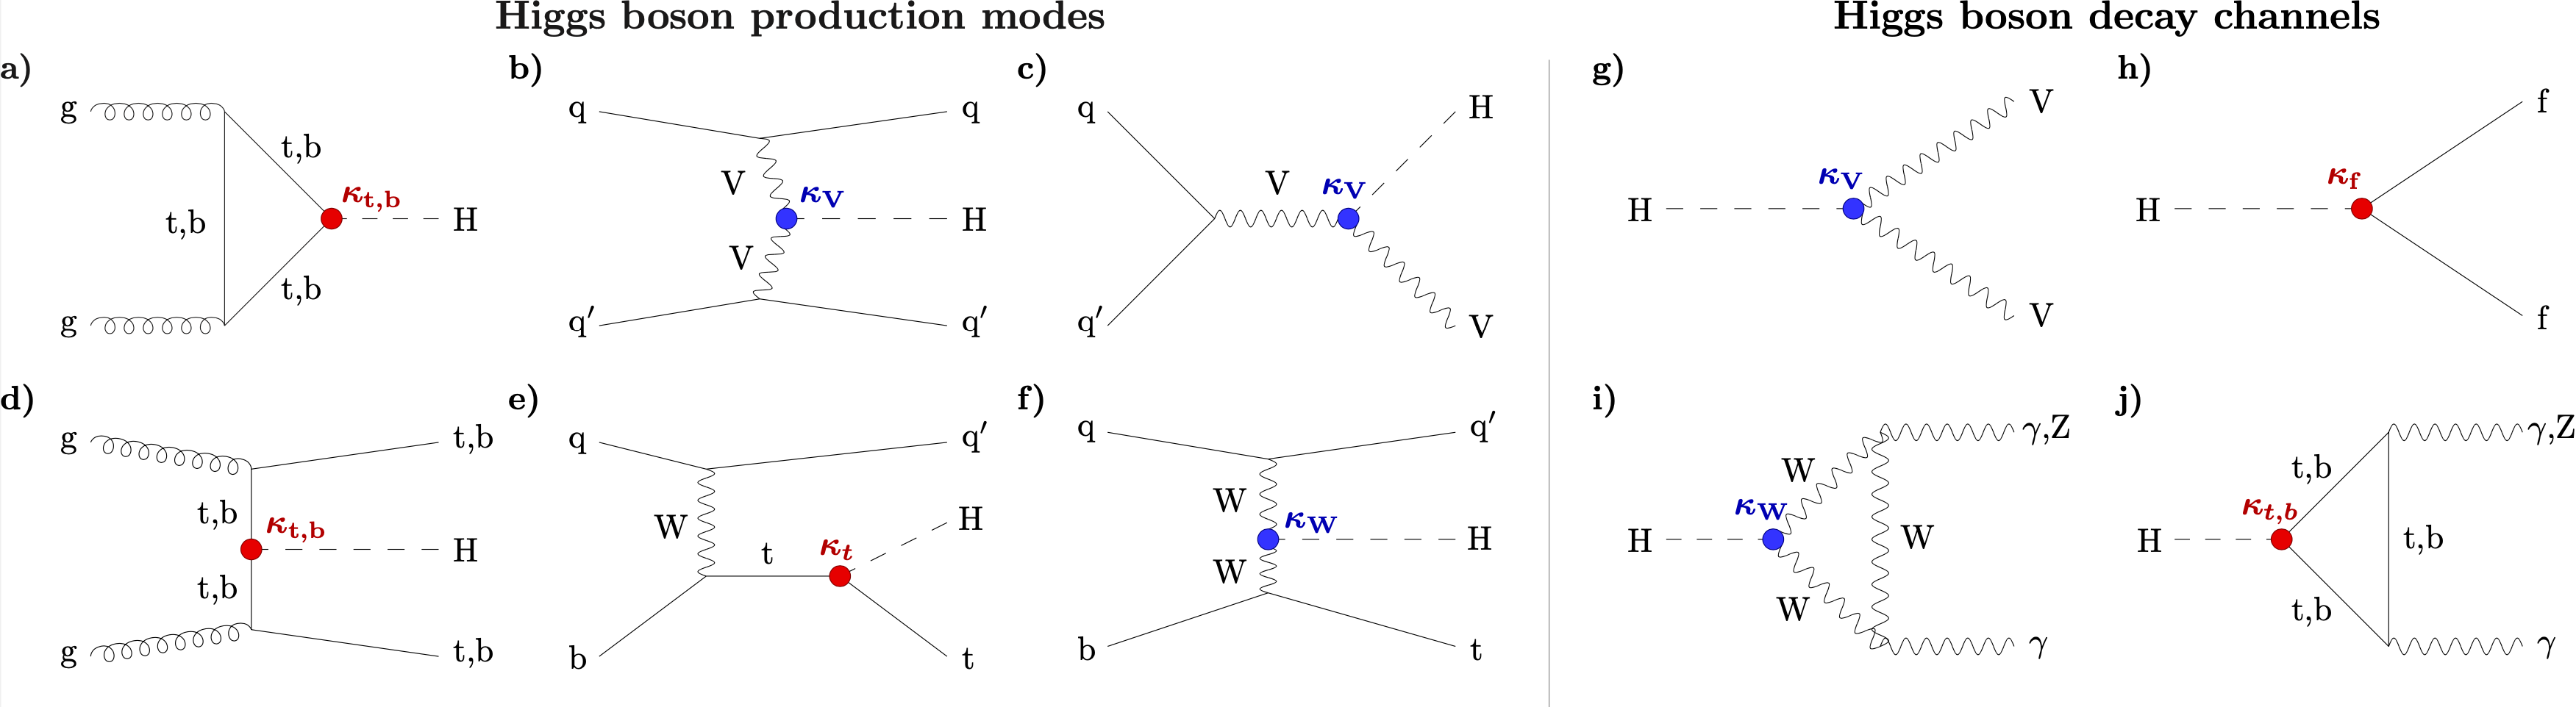
\includegraphics[width=\textwidth]{figures/01-SM-03-SM/higgs/higgs_production.png}
% 	\caption{Single Higgs boson production modes and decay channels at the LHC, reproduced from Ref.~\cite{CMS:2022dwd}.}
% 	\label{fig:01_sm_higgs_production}
% \end{figure}

% \begin{figure}[ht]
% 	\centering
% 	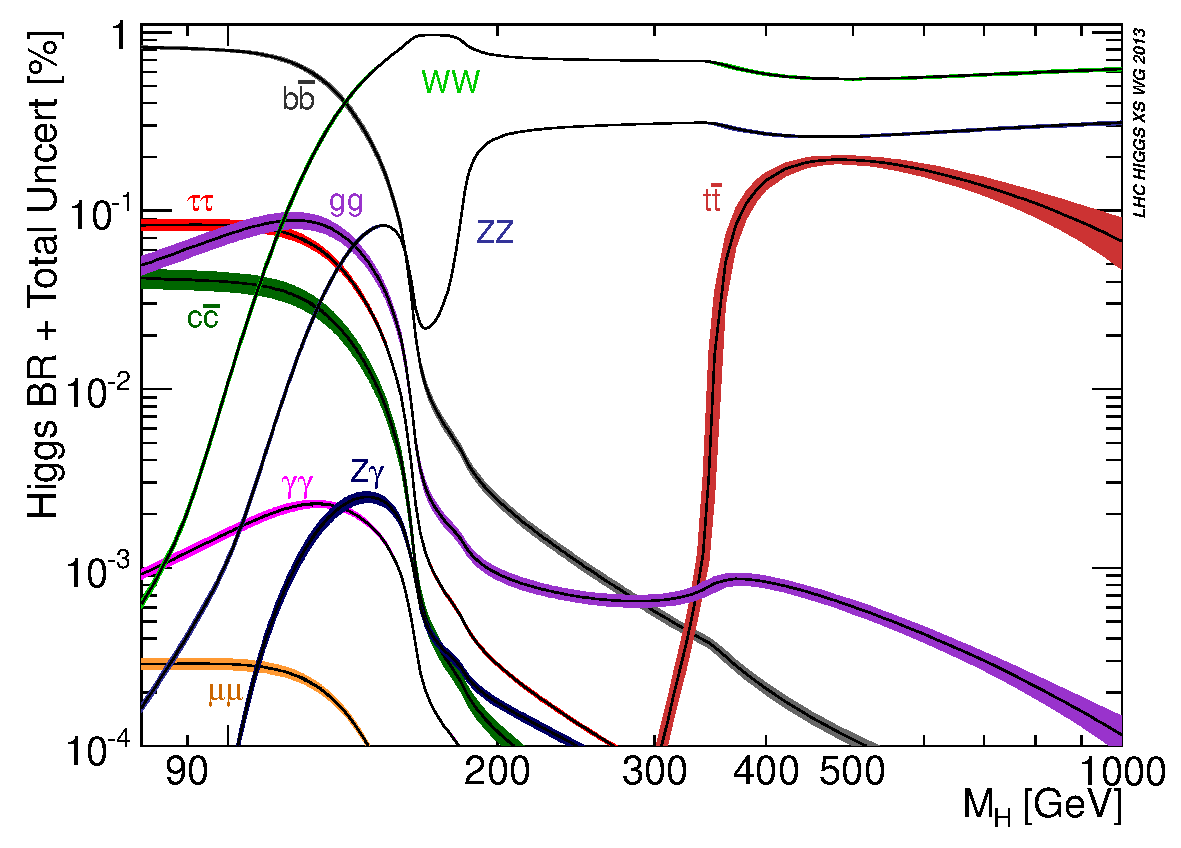
\includegraphics[width=0.8\textwidth]{figures/01-SM-03-SM/higgs/Higgs_BR_RECT.pdf}
% 	\caption{Higgs branching fractions predicted in the SM as a function of \mh (reproduced from Refs.~\cite{Dittmaier:2012vm,LHCHiggsCrossSectionWorkingGroup:2016ypw}).}
% 	\label{fig:01_sm_higgs_hbrs}
% \end{figure}

% The Higgs boson was initially observed by the CMS and ATLAS experiments in 2012 through a combination of several decay channels.
% Since then, the two experiments have been making steady progress in the precise measurements of the various Higgs properties.
% For example, Figure~\ref{fig:01_sm_higgs_constraints} shows the overall constraints on the Higgs to fermion and vector boson couplings and the Higgs mass by the CMS experiment.
% Constraints are based on the $\kappa$-framework~\cite{LHCHiggsCrossSectionWorkingGroup:2013rie}, where $\kappa_X$ scales the Higgs-$X$ coupling strength with $\kappa_X = 1$ corresponding to the SM prediction.
% Changes to the coupling strength due to new physics are thus generically captured by deviations from $\kappa_X = 1$.


% \begin{figure}[ht]
% 	\centering
% 	\adjustbox{valign=m}{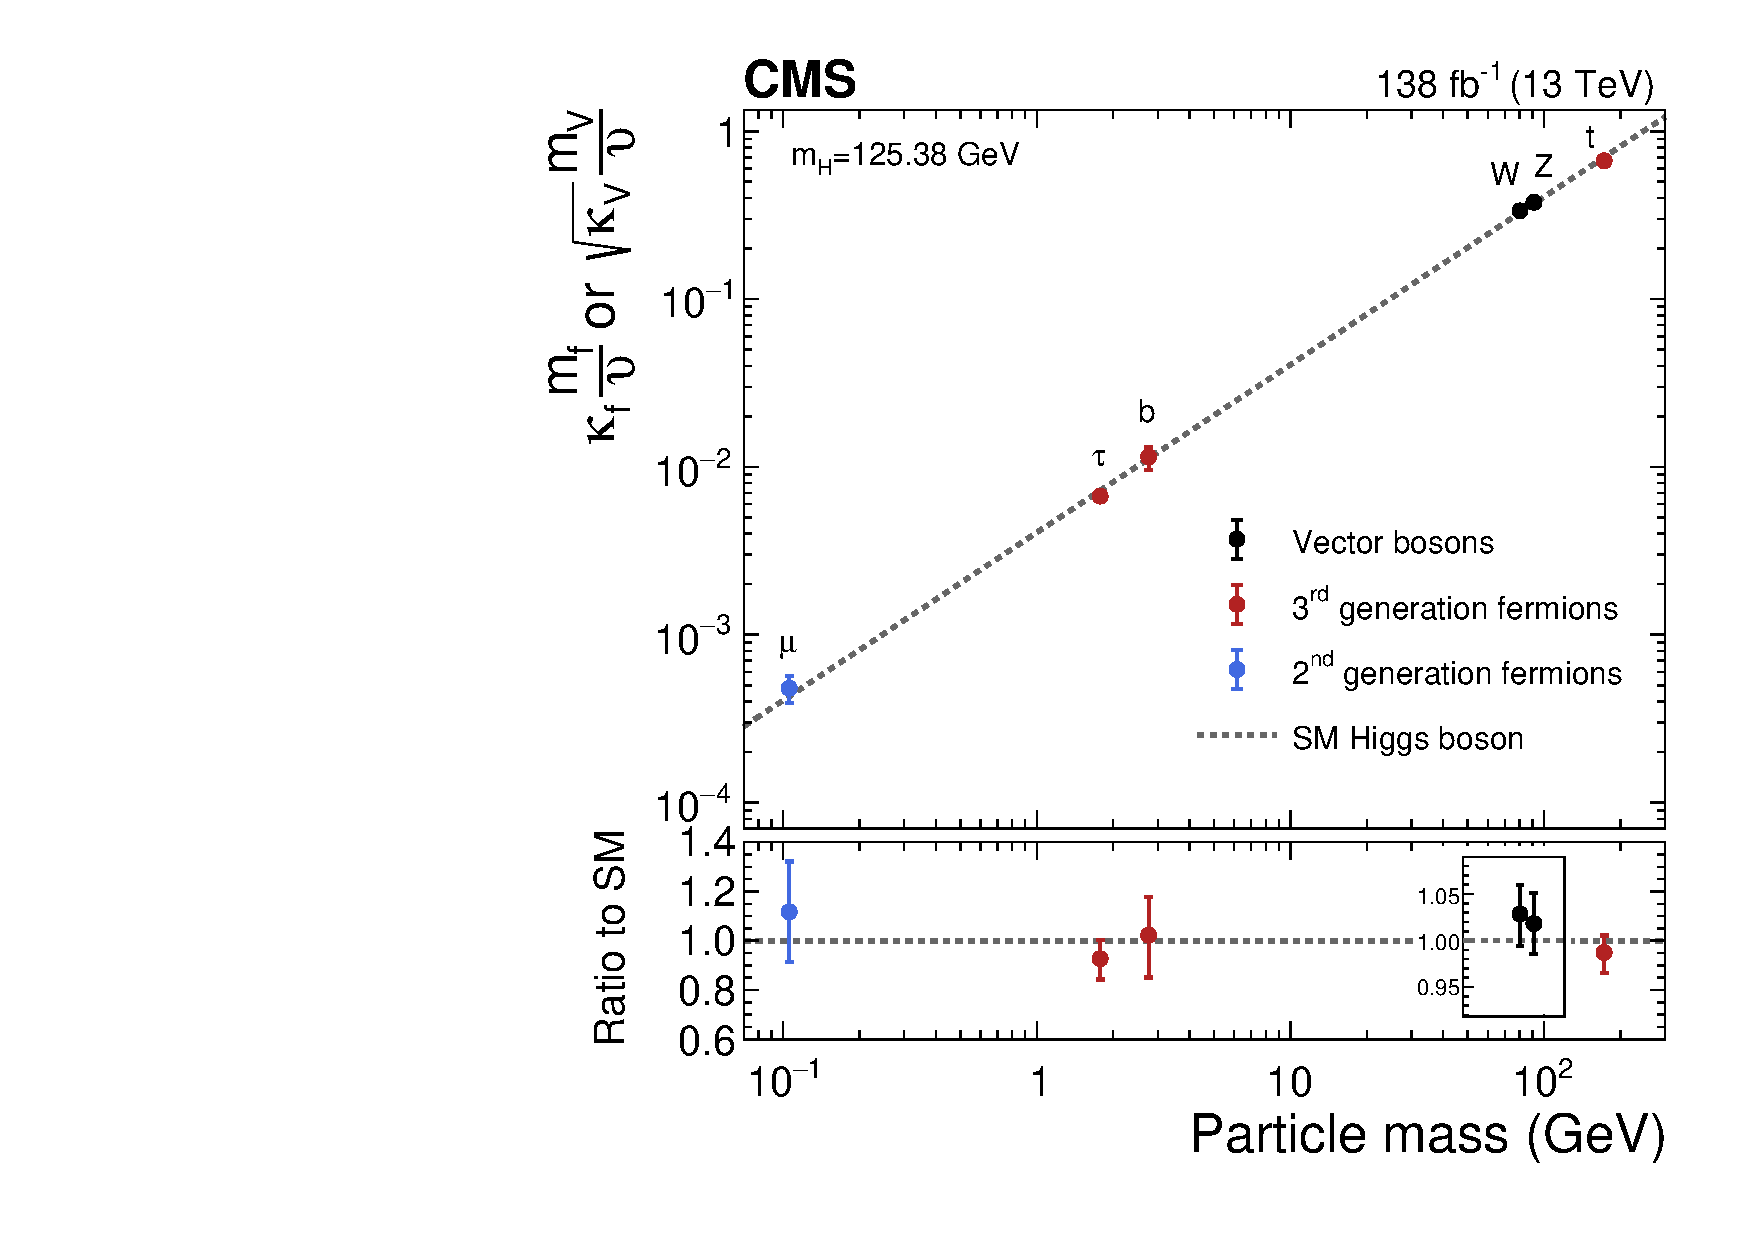
\includegraphics[width=0.49\textwidth]{figures/01-SM-03-SM/higgs/higgs_couplings.pdf}}
% 	\adjustbox{valign=m}{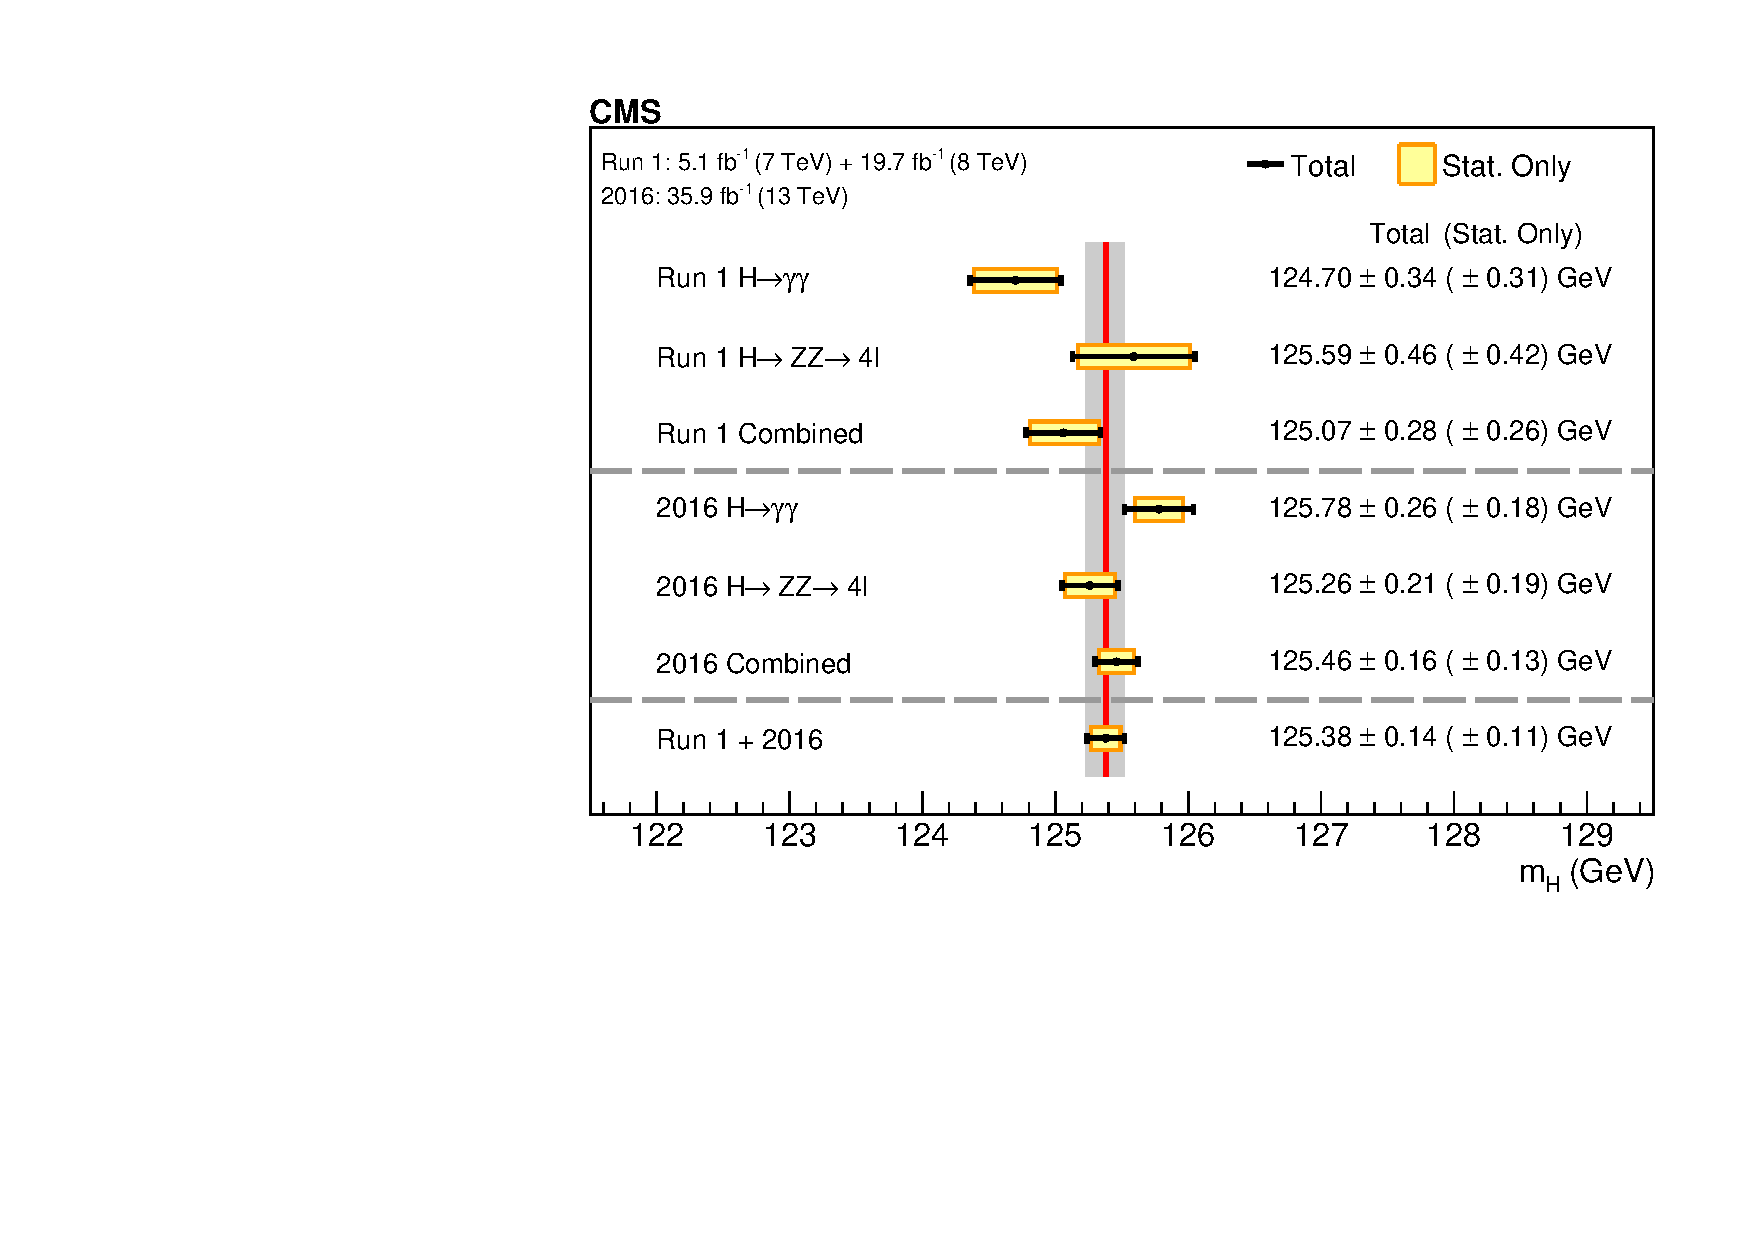
\includegraphics[width=0.49\textwidth]{figures/01-SM-03-SM/higgs/higgs_mass.pdf}}
% 	\caption{Constraints on Higgs to fermion and vector boson couplings, reproduced from Ref.~\cite{CMS:2022dwd} (left) and measurements of the Higgs mass, reproduced from Ref.~\cite{CMS:2020xrn} (right) by the CMS experiment.}
% 	\label{fig:01_sm_higgs_constraints}
% \end{figure}


% \subsection{Higgs pair production in the SM}
% \label{sec:05_smhh}

% Two couplings of the Higgs boson which have not been well-constrained are the trilinear Higgs self-coupling (\HHH), with coupling modifier \kapl, and the Higgs quartic coupling to vector bosons (\HHVV), with modifier $\kapvv$.
% As discussed in Section~\ref{sec:01_sm_ew_ewsb} and illustrated in Figure~\ref{fig:01_sm_higgs_potential}, measuring the Higgs self-coupling in particular is necessary to fully characterize the Higgs potential, deviations to which could hint at BSM explanations to mysteries such as baryon asymmetry~\cite{Reichert:2017puo}.
% As we describe below, both couplings can be probed exclusively through Higgs pair production (\HH), which is why it is a key physics target for the upcoming high-luminosity era of the LHC.

% \begin{figure}[ht]
% 	\centering
% 	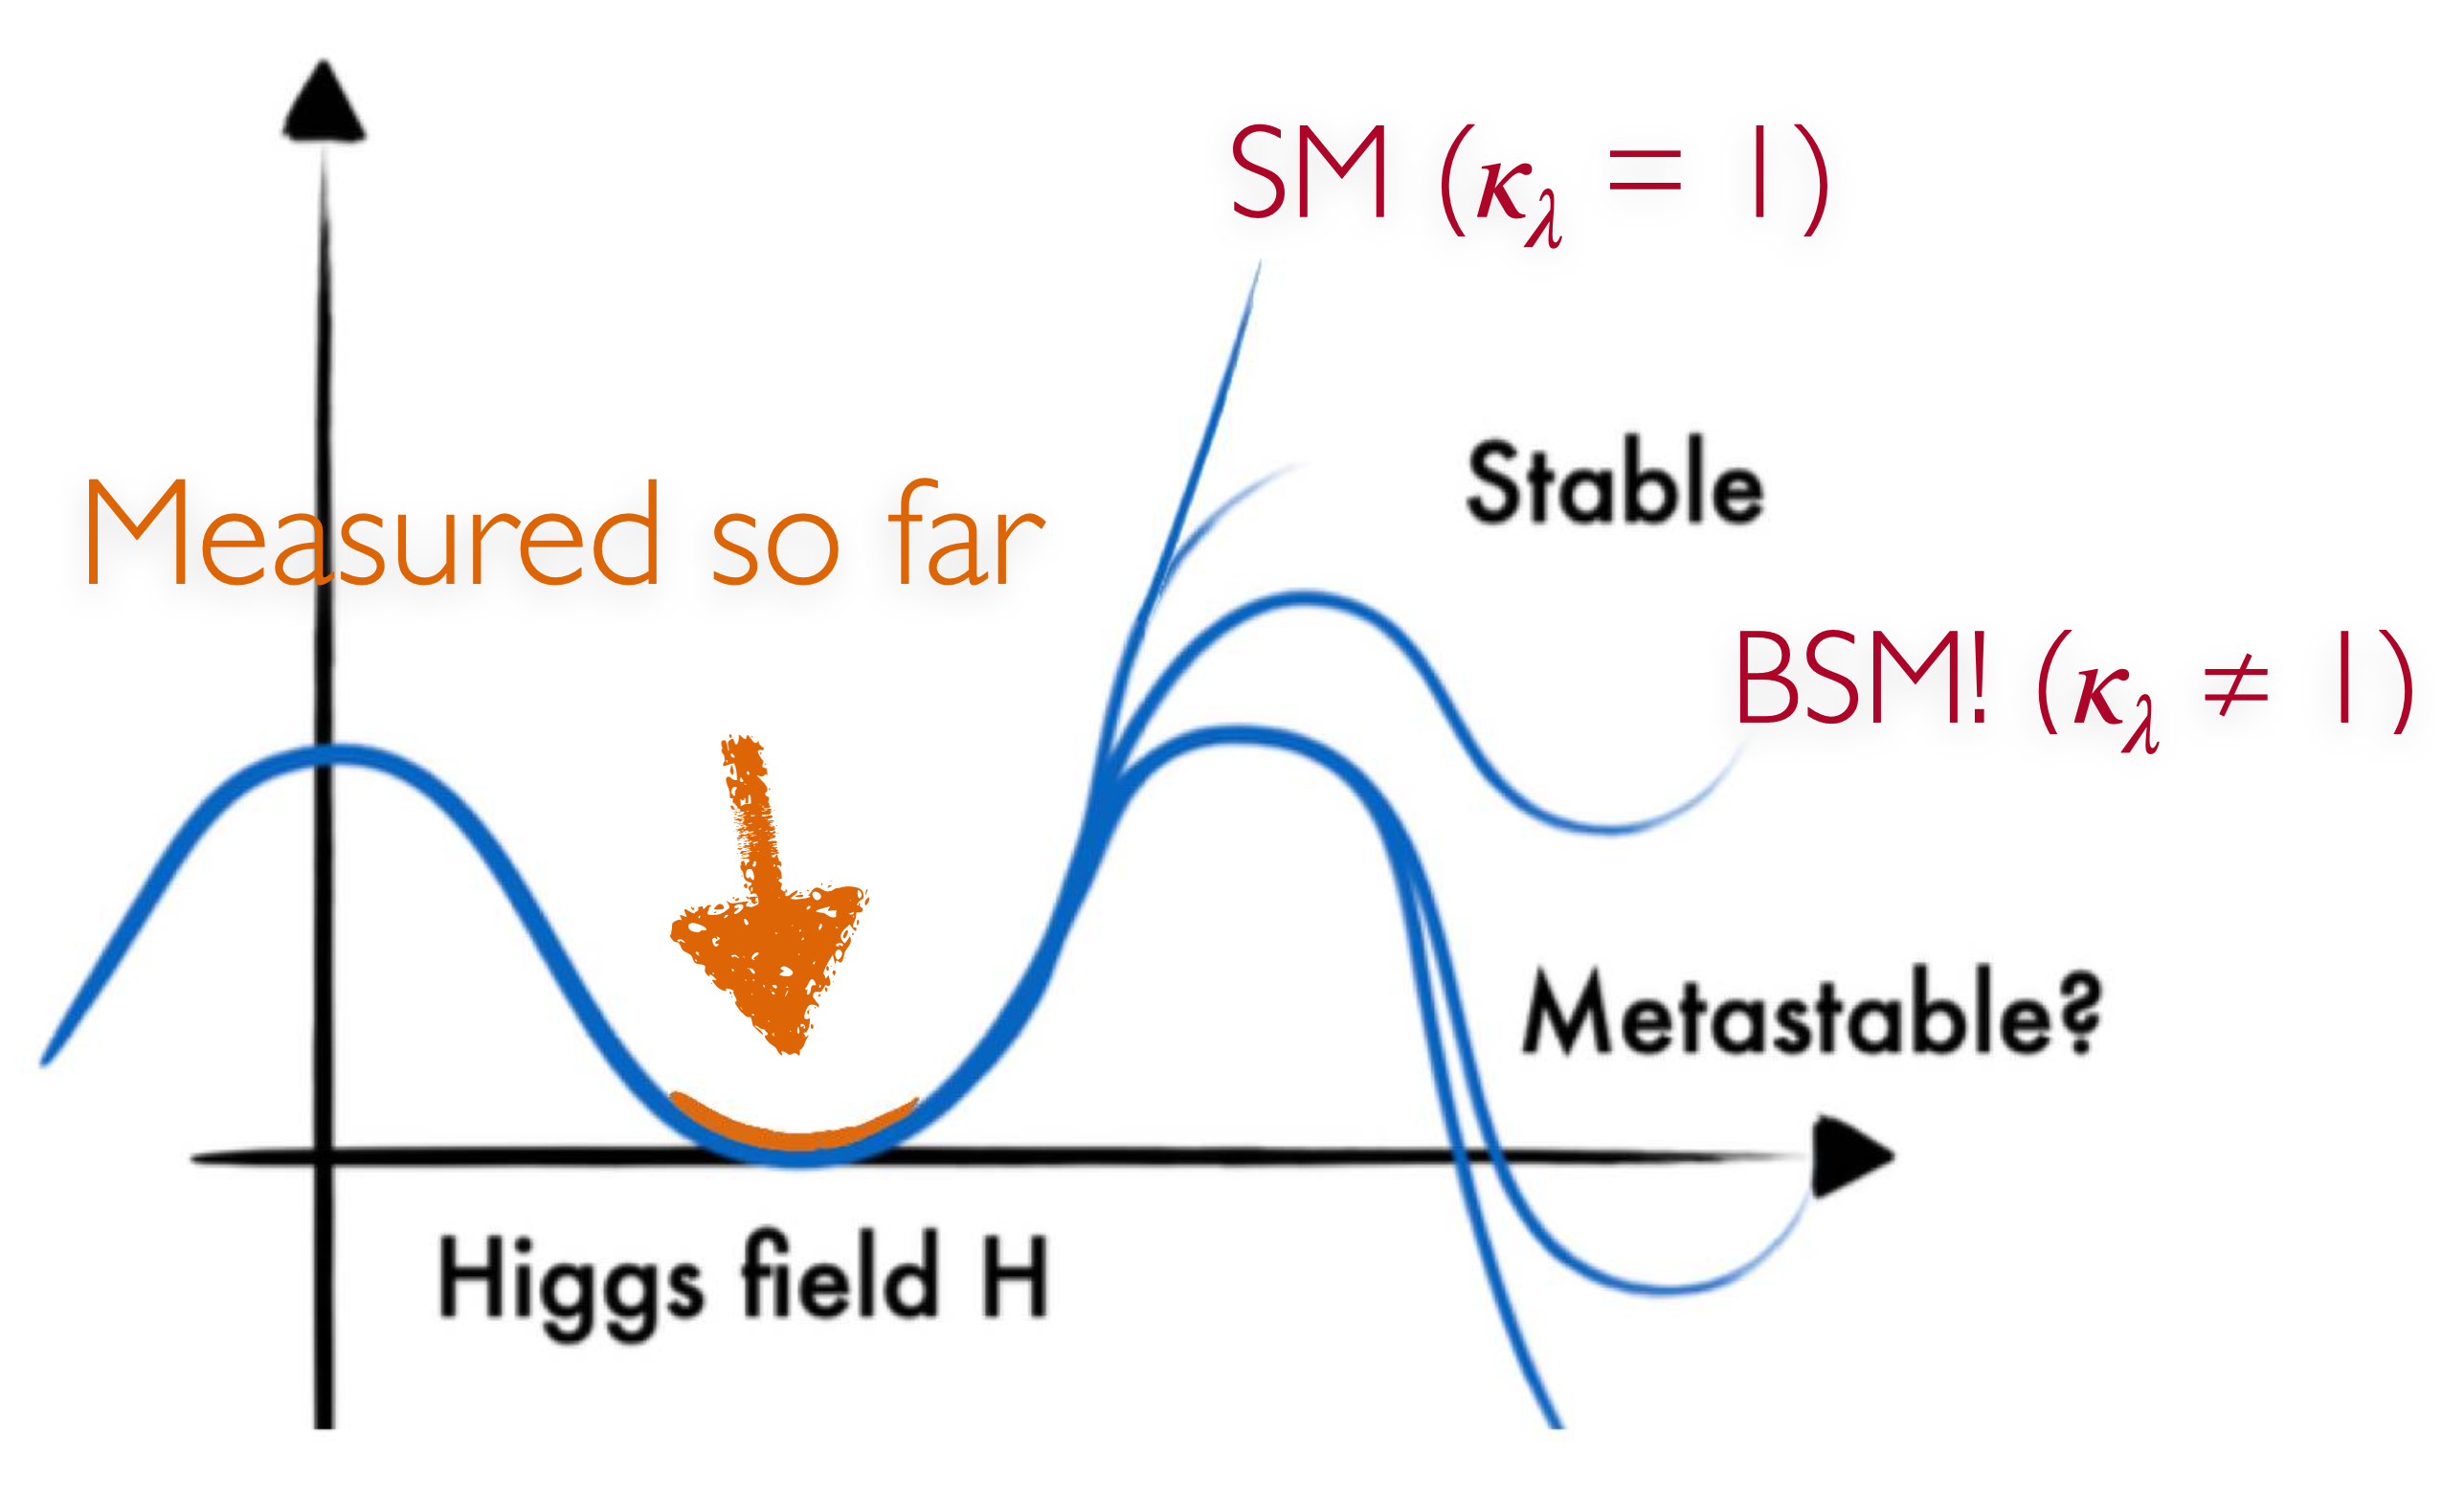
\includegraphics[width=0.5\textwidth]{figures/01-SM-03-SM/higgs/higgs_potential}
% 	\caption{Cartoon of the Higgs potential in the SM and potential deviations due to BSM physics.}
% 	\label{fig:01_sm_higgs_potential}
% \end{figure}

% \HH production in the SM occurs dominantly through gluon fusion (ggF), with a small production cross section $\sigma_\mathrm{ggF} = 31.05^{+2.2\%}_{-5.0\%} \pm 3\% (\textrm{PDF}+\alpS)^{+4\%}_{-18\%} (m_\PQt)\unit{fb}$~\cite{Grazzini:2018bsd,Baglio:2020wgt} at a center of mass energy of 13\TeV and $\mH = 125\GeV$, and subdominantly through vector boson fusion (VBF), with a smaller production cross section $\sigma_\mathrm{VBF} = 1.726^{+0.03\%}_{-0.04\%} \pm 2.1\% (\textrm{PDF}+\alpS)\unit{fb}$~\cite{LHCHiggsCrossSectionWorkingGroup:2016ypw}.
% At leading order, the ggF production mode has contributions from diagrams that involve the trilinear \HHH Higgs self-coupling and the emission of two Higgs bosons through a top quark loop, while the VBF production mode has contributions from three diagrams involving the trilinear \HHH, \HVV, and quartic \HHVV couplings (Figures~\ref{fig:05_feynmanggf} and~\ref{fig:05_feynmanvbf}).
% It also features the distinct final state signature of two, typically forward, jets in addition to the two Higgs bosons.

% \begin{figure}[htb] %[ht]
%     \centering
%     \includegraphics[width=0.4\textwidth]{figures/05-HH/production/diagrams/feynman_02.pdf}
%     \includegraphics[width=0.4\textwidth]{figures/05-HH/production/diagrams/feynman_01.pdf}
%     \caption{Leading-order diagrams for nonresonant \HH production via gluon gluon fusion.}
%     \label{fig:05_feynmanggf}
% \end{figure}  
    
% \begin{figure}[htb]
%     \centering
%     \includegraphics[width=0.32\textwidth]{figures/05-HH/production/diagrams/feynman_04.pdf}
%     \includegraphics[width=0.32\textwidth]{figures/05-HH/production/diagrams/feynman_05.pdf}
%     \includegraphics[width=0.32\textwidth]{figures/05-HH/production/diagrams/feynman_03.pdf}
%     \caption{Leading-order diagrams for nonresonant \HH production via vector boson fusion.
%     In this chapter, we refer to the left-most VBF diagram as the $(\HVV)^2$ and the right-most as the $\HHVV$ diagram.}
%     \label{fig:05_feynmanvbf}
% \end{figure} 

% The production cross section and kinematic properties of the \HH system are altered if values of the Higgs self-coupling, the top Yukawa coupling, and/or the quartic \HHVV coupling are modified due to beyond the SM (BSM) effects.
% Notably, at the energy scale of the LHC, the leading contribution to the VBF production amplitude is the scattering of longitudinal vector bosons, which scales as $\sim \mHH^2 (\kapvv - \kapv^2)$~\cite{Bishara:2016kjn}, where, as above, \kapl, $\kapvv$, and $\kapv$ are defined to be multiplicative modifiers of the \HHH, \HHVV, and \HVV couplings from their SM values, respectively.

% In the SM, with $\kapvv = \kapv = 1$, VBF production is suppressed since the left-most $(\HVV)^2$ and right-most \HHVV VBF diagrams in Figure~\ref{fig:05_feynmanvbf} cancel; however, BSM deviations to \HHVV can spoil the cancelation, significantly enhancing this mode.
% This departure from the SM could be more visible at high energies, as illustrated in Figure~\ref{fig:05_intro_mhh}, which shows the increase and shift towards higher \mHH of the differential VBF \HH production cross section for enhanced and reduced \kapvv values.
% Thus, measuring high-\mHH nonresonant VBF \HH production, with both Higgs bosons highly Lorentz-boosted, is a powerful probe of the \HHVV coupling.

% \begin{figure}[ht]
%     \centering
%     \includegraphics[width=0.7\textwidth]{figures/05-HH/production/diagrams_prelim.pdf}
%     \caption{Differential cross section at $13\TeV$ center of mass for VBF \HH production as a function of the invariant mass of the \HH system (\mHH) for different diagrams and couplings.}
%     \label{fig:05_intro_mhh}
% \end{figure}

% This is evidenced by the current \kapvv constraint in CMS being dominated by the search for boosted \HH in the \bbbb channel, with an observed (expected) 95\% confidence level (\CL) constraint of $[0.6, 1.4]$ ($[0.7, 1.4]$), excluding $\kapvv = 0$ for the first time~\cite{CMS:2022gjd}.
% This is followed by CMS searches in the resolved \bbbb~\cite{CMS:2022cpr} and \bbtautau~\cite{CMS:2022hgz} channels, with constraints of $[-0.1, 2.2]$ ($[-0.4, 2.5]$) and $[-0.4, 2.6]$ ($[-0.6, 2.8]$), respectively.
% Similarly, the strongest \kapvv constraint from the ATLAS experiment is from the boosted \bbbb search~\cite{ATLAS-CONF-2024-003}, with an observed (expected) 95\% \CL constraint of $[0.55, 1.49]$ ($[0.3, 1.7]$).

% The success of searches in the boosted \bbbb channel motivates further exploration of high-\mHH \HH production.
% This dissertation presents the first search in the all-hadronic \bbvv channel, where one Higgs boson decays to \bbbar while the other to \ww or \zz, where $\PW\to\qqbar$ and $\PZ\to\qqbar$.
% The branching fractions for the \bbbar and all-hadronic \vv decays are $0.58$ and $0.11$ respectively, for a total branching fraction $\mathcal{B}(\HHbbVVq) = 2  \cdot0.58\cdot 0.11 = 0.13$, which is the second largest behind \bbbb.
% The analysis primarily aims to constrain \kapvv and also sets an exclusion limit on the inclusive \HH production cross-section.
% It is not expected to be sensitive to \kapl because of the focus on the high-\mHH regime.

% Another benefit of the high-\mHH regime is the significantly reduced QCD multijet background, which otherwise makes such all-hadronic searches extremely challenging.
% Because of the two Higgs bosons' high Lorentz-boosts, this regime also features the unique experimental signature of the \bbbar and \vvq decays each being reconstructed as single wide-radius jets.
% Such merged \hbb jets have been identified to great effect in CMS using deep neural networks (DNNs)~\cite{CMS:2023tlv, CMS:2022gjd}, but attaining similar signal versus background discrimination for \hvv jets remains an open challenge.
% To this end, we introduce a new attention-based DNN, referred to as the global particle transformer (GloParT) to not only enable this search but open new possibilities for searches in boosted-\vv channels as well (Chapter~\ref{sec:05_jet_tagging}).

% \subsection{Experimental status of \HH measurements with CMS}
% \label{sec:05_smhh_golden_channels}

% \begin{figure}[ht]
%     \centering
%     % \captionsetup{justification=centering}
%     \includegraphics[width=0.6\textwidth]{figures/05-HH/CMS-results/HHBRs.png}
%     \caption{\HH decays and their respective branching fractions (reproduced from Ref.~\cite{Veatch:2022uzz}).}
%     \label{fig:05_hhbrs}
% \end{figure}

% The decays and branching fractions (BFs) of the Higgs boson pairs are shown in Figure~\ref{fig:05_hhbrs}.
% Three of these final states have emerged as experimental ``golden channels'' --- the channels expected to yield the highest signal-to-background-events ratio for SM \HH production:
% \begin{itemize}
%     \item \bbbb:\quad This channel has the highest BF ($34\%$) and, despite the large QCD multijet background due to the all-hadronic final state, it benefits from unique signatures of heavy-flavor \Pb-jets, such as the presence of secondary vertices and displaced tracks due to the long lifetimes of \Pb-hadrons.
%     Both the resolved~\cite{CMS:2022cpr} and boosted~\cite{CMS:2022gjd} Run 2 CMS analyses (Figure~\ref{fig:05_bbbb_run2}) have been highly effective, with the latter benefitting from the high BF of this decay mode, the exponential reduction of the QCD multijet background in the boosted regime, and significant recent advances in \bbbar-jet classification and reconstruction (as will be discussed in Chapter~\ref{sec:05_jet_tagging}). 
%     \item \bbtautau:\quad This has an intermediate BF of $7\%$ but relatively lower background of primarily Drell-Yan ($\PZ/\PGg^*$), top quark pair production (\ttbar), and QCD multijet events (Figure~\ref{fig:05_bbtautau}, reproduced from Ref.~\cite{CMS:2022hgz}).
%     It benefits from similar deep learning techniques for \Pb-jet tagging, and targets all-hadronic ($\PGt_h\PGt_h$) and semi-leptonic ($\PGt_h\PGt_e$ or $\PGt_h\PGt_\mu$) \PGt-lepton decays using a variety of traditional and ML techniques.
%     \item \bbgg:\quad Despite the small BF ($0.3\%$) of this channel, the $\PH\to\PGg\PGg$ decay provides a clean experimental signature with a sharply peaking resonance over a small background of QCD multijet + $\PGg$ events (Figure~\ref{fig:05_bbgg}, from Ref.~\cite{CMS:2020tkr}).
% \end{itemize}

% More recently, the \bbww channel has been explored in the douple-lepton ($\Pl\Pl\nu\nu$) and single-lepton ($\Pl\nu\Pq\Pq$) \ww final states~\cite{CMS:2024rgy}, which have a large combined BF of $13.4\%$.
% The former features a clean experimental signature of two opposite-sign leptons but a small BF of $2.6\%$, while the latter has the higher BF of 10.8\% but larger top quark background as well (Figure~\ref{fig:05_bbww}).
% Because of this, the two channels have similar sensitivities to the \HH cross section.

% \begin{figure}[htb!]
%     \centering
%     \includegraphics[trim=260pt 20pt 40pt 20pt, clip, width=0.31\textwidth]{figures/05-HH/CMS-results/4b/Figure_001-e.png}
%     \includegraphics[width=0.33\textwidth]{figures/05-HH/CMS-results/4b/Figure_001-a.pdf}
%     \includegraphics[width=0.33\textwidth]{figures/05-HH/CMS-results/4b/Figure_002.pdf}
%     \caption[Distribution of events in the high-\mHH ggF category of the Run 2 CMS $\HH\to\bbbb$ resolved analysis~\cite{CMS:2022cpr}.]{Distribution of events in the high-\mHH ggF category of the Run 2 CMS $\HH\to\bbbb$ resolved analysis~\cite{CMS:2022cpr} as a function of the BDT discriminant (left), and of the Run 2 boosted analysis'~\cite{CMS:2022gjd} most sensitive ggF category, as a function of the second-highest tagged \bbbar-jet's mass (middle), and VBF categories, as a function of \mHH (right).}
%     \label{fig:05_bbbb_run2}
% \end{figure}

% \begin{figure}[htb!]
%     \centering
%     \includegraphics[trim=270pt 120pt 30pt 20pt, clip, width=0.32\textwidth]{figures/05-HH/CMS-results/bbtautau/Figure_005-a.png}
%     \includegraphics[trim=270pt 120pt 30pt 20pt, clip, width=0.32\textwidth]{figures/05-HH/CMS-results/bbtautau/Figure_005-b.png}
%     \includegraphics[trim=270pt 120pt 30pt 20pt, clip, width=0.32\textwidth]{figures/05-HH/CMS-results/bbtautau/Figure_005-c.png}
%     \caption{Combination of bins of all postfit distributions of the Run 2 CMS $\HH\to\bbtautau$ analysis~\cite{CMS:2022hgz}, ordered according to the expected signal-to-square-root-background ratio, separately for the $\PGt_h\PGt_e$ (left), the $\PGt_h\PGt_\mu$ (center), and $\PGt_h\PGt_h$ (right) channels.}
%     \label{fig:05_bbtautau}
% \end{figure}

% \begin{figure}[htb!]
%     \centering
%     \includegraphics[trim=250pt 25pt 0 20pt, clip, width=0.5\textwidth]{figures/05-HH/CMS-results/bbgg.png}
%     \caption[Invariant two-photon mass distribution of the Run 2 CMS $\HH\to\bbgg$ analysis~\cite{CMS:2020tkr}.]{Invariant two-photon mass distribution of the Run 2 CMS $\HH\to\bbgg$ analysis~\cite{CMS:2020tkr}, combined for all signal categories, weighted by S/(S+B), where S (B) is the number of signal (background) events extracted from the signal-plus-background fit.}
%     \label{fig:05_bbgg}
% \end{figure}

% \begin{figure}[htb!]
%     \centering
%     \includegraphics[width=0.49\textwidth]{figures/05-HH/CMS-results/bbww/Figure_006-a.pdf}
%     \includegraphics[width=0.49\textwidth]{figures/05-HH/CMS-results/bbww/Figure_006-b.pdf}
%     \caption[Distribution of events in the resolved $1\Pb$, resolved $\geq2\Pb$, and boosted signal categories of the Run 2 CMS semi-leptonic $\HH\to\bbww$ analysis~\cite{CMS:2024rgy}.]{Distribution of events in the resolved $1\Pb$, resolved $\geq2\Pb$, and boosted signal categories of the Run 2 CMS semi-leptonic $\HH\to\bbww$ analysis~\cite{CMS:2024rgy} as a function of their DNN discriminant in the single-lepton (left) and double-lepton (right) final states.}
%     \label{fig:05_bbww}
% \end{figure}

% The limits set on the \HH cross section by each channel, and their combinations, are shown in Figure~\ref{fig:05_hh_comb_xsec}, and as a function of \kapl and \kapvv in Figure~\ref{fig:05_hh_comb_kappa}.
% The three ``golden channels'' each offer roughly similar sensitivities to the cross section and \kapl limits; however, the constraint on \kapvv is dominated by the boosted \bbbb channel, because of the enhancement of boosted \HH production at BSM \kapvv deviations, as discussed in Section~\ref{sec:05_smhh}.
% Its observed (expected) $95\%$ confidence level (\CL) constraint is $[0.6, 1.4]$ ($[0.7, 1.4]$).
% This is followed by the resolved \bbbb~\cite{CMS:2022cpr} and \bbtautau~\cite{CMS:2022hgz} channels, with constraints of $[-0.1, 2.2]$ ($[-0.4, 2.5]$) and $[-0.4, 2.6]$ ($[-0.6, 2.8]$), respectively.
% Similarly, the strongest \kapvv constraint from the ATLAS experiment is from the recent boosted \bbbb search~\cite{ATLAS-CONF-2024-003}, with an observed (expected) $95\%$ \CL constraint of $[0.55, 1.49]$ ($[0.3, 1.7]$).

% \begin{figure}[htb!]
%     \centering
%     \includegraphics[width=0.8\textwidth]{figures/05-HH/CMS-results/HHcomb_xsec.pdf}
%     \caption[The expected and observed limits on the ratio of experimentally estimated production cross section and the expectation from the SM in searches using different final states and their combination, reproduced from Ref.~\cite{CMS-PAS-HIG-20-011}.]{The expected and observed limits on the ratio of experimentally estimated production cross section and the expectation from the SM in searches using different final states and their combination, reproduced from Ref.~\cite{CMS-PAS-HIG-20-011}. 
%     The search modes are ordered, from upper to lower, by their expected sensitivities from the least to the most sensitive. The overall combination of all searches is shown by the lowest entry.}
%     \label{fig:05_hh_comb_xsec}
% \end{figure}

% \begin{figure}[htb!]
%     \centering
%     \includegraphics[width=0.49\textwidth]{figures/05-HH/CMS-results/kl_limits_channels_r_paper.pdf}
%     \includegraphics[width=0.49\textwidth]{figures/05-HH/CMS-results/C2V_limits_channels_rqqHH_paper.pdf}
%     \caption[The expected and observed limits on the ratio of experimentally estimated production cross section and the theory expectation.]{The expected and observed limits on the ratio of experimentally estimated production cross section and the theory expectation for different values of \kapl (left) and \kapvv (right), reproduced from Ref.~\cite{CMS-PAS-HIG-20-011}.}
%     \label{fig:05_hh_comb_kappa}
% \end{figure}


% In this dissertation, we present the first search for nonresonant \HH production in the \textit{all-hadronic \bbvv channel}, where one Higgs decays to two bottom quarks, while the other to two vector bosons (\vv) both decaying hadronically to the four quark (\qqqq) final state.
% Both the \PW and \PZ bosons are considered for the latter decay and collectively referred to as \PV bosons.
% The branching fractions for the \bbbar and \vv decays are $0.58$ and $0.25$ respectively, for a total branching fraction $\mathcal{B}(\HHbbVV) = 2  \cdot0.58\cdot 0.25 = 0.29$, which is the second-highest, behind only \bbbb. 
% The all-hadronic final state in particular has a branching fraction of $0.13$. 
% The analysis targets the boosted regime, which, as discussed above, has the two-fold advantage of 1) increasing sensitivity to \kapvv deviations and 2) exponentially reducing the dominant QCD multijet background.



% \subsection{BSM \texorpdfstring{\XHY}{X→HY} production}
% \label{sec:05_bsmxhy}

% \begin{figure}[htb] %[ht]
%     \centering
%     % \captionsetup{justification=centering}
%     \includegraphics[width=\textwidth]{figures/05-HH/production/xhy.png}
%     \caption{\XHY production in the symmetric (left) and asymmetric (right) cases.}
%     \label{fig:05_xhy_production}
% \end{figure} 

% Many theoretical models predict a richer scalar sector than that in the SM to address aesthetic and observational inconsistencies with the SM, such as the Higgs mass hierarchy problem and the baryon asymmetry discussed above.
% These include two-Higgs doublet models (2HDM)~\cite{Branco:2011iw} that add an additional scalar doublet to the SM, such as the minimal supersymmetric extension of the SM (MSSM)~\cite{Craig:2013hca}, which predicts two neutral CP-even scalars (\PH, \Ph), one neutral CP-odd scalar (\PA), and two charged scalars ($\PH^\pm$), where one of the neutral CP-even scalars may be the discovered SM Higgs \PHsm.
% The next-to-minimal supersymmetric extension of the SM (NMSSM)~\cite{Domingo:2022kfm} adds to this a complex scalar singlet, predicting two more CP-even ($\Ph_\mathrm{s}$) and CP-odd ($\Pa_\mathrm{s}$) neutral scalars.
% Finally, the two-real-singlet-model (TRSM) predicts two additional CP-even scalar fields.
% Depending on the kinematics, all these models allow for cascade decays of a heavier scalar to symmetric and asymmetric lighter scalars, such as $\PH\to\PHsm\PHsm$ and $\PH\to\Ph\PHsm$, respectively, as shown in Figure~\ref{fig:05_xhy_production}.

% We search for this broad class of signals, looking for generic decays of the form \XHY, where \PX is the heavier and \PY the lighter scalar resonance, with \PH decaying to \bbbar and \PY to \vvq. 
% Many models, such as the TRSM, predict branching ratios for the lighter scalar similar to or the same as the SM Higgs.
% In this case, the \vv decay modes are dominant for $\my > 140\GeV$ (Figure~\ref{fig:01_sm_higgs_hbrs}) and, hence, the \hbb and \yvv will be the dominant final states for the \XHY signal.
% Thus, the \bbvv channel represents the highest BF in these models.

% There are several published and ongoing CMS searches for \XHY production in a variety of regimes and final states with the Run 2 dataset, such as the boosted~\cite{BoostedXHY4b} \bbbb final state, the symmetric-only $\bbbar\PW\PW$ semi-leptonic final state~\cite{CMS:2024rgy}, the resolved $\bbbar\PGg\PGg$~\cite{CMS:2023boe}, and the resolved $\bbbar\PGt\PGt$~\cite{CMS:2021yci} final state. 
% This dissertation presents the first search in the \bbvv all-hadronic state, and the first in the \bbvv state for the asymmetric case, representing a significant increase in the covered phase space for \XHY searches.

% The search comprises two distinct topologies depending on the ratio of the \PX and \PY masses: a highly-boosted fully-merged \yvv topology for $\mx \gg \my$, with both \vv bosons' decay products highly collimated into a single wide-radius jet; and a relatively less-boosted semi-merged topology, where the \vv bosons are well separated and each \vqq decay is reconstructed as its own wide-radius jet.
% These two phases are illustrated in Figure~\ref{fig:05_xhy_fraction_3q4q}, showing the fraction of \yvv jets containing three or four generator-level quarks as a function of the \PX and \PY boson masses, with the transition occurring around $\mx \approx 10\my$.
% This dissertation focuses on a search for the fully-merged topology only, i.e. for $\mx \gtrsim 10\my$, and is complementary to an ongoing CMS search in the semi-merged topology.
% Thus, in terms of the analysis strategy and techniques, this search is similar to the boosted nonresonant \HH search in that they both target highly-boosted Higgs decays with single wide-radius jets for both \PH and/or \PY bosons.

% \begin{figure}[htb] %[ht]
%     \centering
%     % \captionsetup{justification=centering}
%     \includegraphics[width=0.8\textwidth]{figures/05-HH/production/fraction_3q4q.pdf}
%     \caption{The fraction of \yvv jets containing three or four generator-level quarks for the resonant \XHYbbVV signal as a function of the \PX and \PY boson masses.}
%     \label{fig:05_xhy_fraction_3q4q}
% \end{figure} 


% As shown in Figure~\ref{fig:01_sm_higgs_production}, both couplings can be accessed at the LHC exclusively through Higgs pair production.
% This dissertation describes one such measurement by the CMS experiment in the \bbvv channel, which is particularly sensitive to BSM deviations of the \HHVV coupling.
% It also presents a search for a new heavy resonance decaying to two Higgs bosons in the same channel, as predicted by many BSM theories described in Chapter~\ref{sec:05_bsmxhy}.

% \section{Beyond the Standard Model}

% \subsection{Gravity}

%  - Gravity not a renormalizable QFT, can be thought of as an EFT in powers of (E/Mpl), so will never see the effect \\
%  - Experimentally, almost no consequence, but still fun to think about (although the 15 orders of magnitude gap makes you wonder if we are like the Greeks ``reasoning'' about atoms) \\
%  - String theory --- strings instead of particles, graviton arises, benefits: reproduces GR, SM etc. in the low-energy limit, but lots of unsolved problems \\
%  - Loop quantum gravity --- quantize space-time, only 4D, but so far does not reproduce our theories, interesting cosmological tests (constraint on spacetime quantization) \\
%  - Asymptotic safety --- Don't need gravity to be renormalizable, as long as the coupling constants have UV-safe fixed points (?), progress recently (see Weinberg 2009 lecture on motivation) \\


% \subsection{Grand unification}

%  - ``Zoo'' of particle representations can all be unified into two representations of a larger group SU(5), or even just a single huge representation of SO(10) (similar to two SU(2)'s embedded into SO(3, 1) or SO(4)) \\
%  - Very aesthetically pleasing, but moreover, lots of physical insights: charge quantization, proton charge = electron charge, \\
%  - SO(10) only: anti- / righthanded-neutrino, all fermions are encoded in ``five-bit strings'' (Zee) (although this predicts as-yet-unobserved fermions) \\
%  - Can keep adding bits / increasing the group size to include the different generations as well \\

%  - Similar to theories of quantum gravity, the GUT scale is so high that any effects will not be observed within our lifetimes sadly \\
%  - e.g. proton decay

% \subsection{Dark energy}

%  - Experimental evidence \\
%  - Higgs seesaw mechanism \\

% \subsection{Neutrino masses}

%  - Experimental evidence \\
%  - Seesaw mechanism \\

% \subsection{Dark matter}

%  - Experimental evidence \\
%  - WIMP, axion, sterile neutrinos, etc. \\
%  - Connections to Higgs \\

% \subsection{Baryon asymmetry}

%  - Sakharov conditions \\
%  - Relation to Higgs \\

% \subsection{Hierarchy problem}

%  - Is it a problem? \\
%  - Solutions \\

% \subsection{The SM as an effective field theory}

% HH EFT \\



% \section{Summary}
\end{doublespace}

\nocite{apsrev42Control}
\bibliography{bibliography}
 
\end{document}